\documentclass[a4paper]{book}
\usepackage{makeidx}
\usepackage{graphicx}
\usepackage{multicol}
\usepackage{float}
\usepackage{listings}
\usepackage{color}
\usepackage{ifthen}
\usepackage[table]{xcolor}
\usepackage{textcomp}
\usepackage{alltt}
\usepackage{ifpdf}
\ifpdf
\usepackage[pdftex,
            pagebackref=true,
            colorlinks=true,
            linkcolor=blue,
            unicode
           ]{hyperref}
\else
\usepackage[ps2pdf,
            pagebackref=true,
            colorlinks=true,
            linkcolor=blue,
            unicode
           ]{hyperref}
\usepackage{pspicture}
\fi
\usepackage[utf8]{inputenc}
\usepackage[french]{babel}

\usepackage{mathptmx}
\usepackage[scaled=.90]{helvet}
\usepackage{courier}
\usepackage{doxygen}
\lstset{language=C++,inputencoding=utf8,basicstyle=\footnotesize,breaklines=true,breakatwhitespace=true,tabsize=8,numbers=left }
\makeindex
\setcounter{tocdepth}{3}
\renewcommand{\footrulewidth}{0.4pt}
\begin{document}
\hypersetup{pageanchor=false}
\begin{titlepage}
\vspace*{7cm}
\begin{center}
{\Large DTDLib \\[1ex]\large 0.1 }\\
\vspace*{1cm}
{\large Généré par Doxygen 1.7.2}\\
\vspace*{0.5cm}
{\small Sun Apr 17 2011 19:07:13}\\
\end{center}
\end{titlepage}
\clearemptydoublepage
\pagenumbering{roman}
\tableofcontents
\clearemptydoublepage
\pagenumbering{arabic}
\hypersetup{pageanchor=true}
\chapter{Index des espaces de nommage}
\section{Liste des espaces de nommage}
Liste de tous les espaces de nommage avec une brève description:\begin{DoxyCompactList}
\item\contentsline{section}{\hyperlink{namespacexml}{xml} }{\pageref{namespacexml}}{}
\end{DoxyCompactList}

\chapter{Index des classes}
\section{Hiérarchie des classes}
Cette liste d'héritage est classée approximativement par ordre alphabétique :\begin{DoxyCompactList}
\item \contentsline{section}{xml::InterfaceNodeVisitor}{\pageref{classxml_1_1_interface_node_visitor}}{}
\begin{DoxyCompactList}
\item \contentsline{section}{xml::DotOutputVisitor}{\pageref{classxml_1_1_dot_output_visitor}}{}
\item \contentsline{section}{xml::OutputVisitor}{\pageref{classxml_1_1_output_visitor}}{}
\end{DoxyCompactList}
\item \contentsline{section}{xml::Node}{\pageref{classxml_1_1_node}}{}
\begin{DoxyCompactList}
\item \contentsline{section}{xml::MarkupNode}{\pageref{classxml_1_1_markup_node}}{}
\begin{DoxyCompactList}
\item \contentsline{section}{xml::CompositeMarkupNode}{\pageref{classxml_1_1_composite_markup_node}}{}
\end{DoxyCompactList}
\item \contentsline{section}{xml::TextNode}{\pageref{classxml_1_1_text_node}}{}
\end{DoxyCompactList}
\end{DoxyCompactList}

\chapter{Index des classes}
\section{Liste des classes}
Liste des classes, structures, unions et interfaces avec une brève description :\begin{DoxyCompactList}
\item\contentsline{section}{\hyperlink{structdtd_1_1_choice_1_1___state}{dtd::Choice::\_\-State} }{\pageref{structdtd_1_1_choice_1_1___state}}{}
\item\contentsline{section}{\hyperlink{structdtd_1_1_quantifiable_content_1_1___state}{dtd::QuantifiableContent::\_\-State} }{\pageref{structdtd_1_1_quantifiable_content_1_1___state}}{}
\item\contentsline{section}{\hyperlink{structdtd_1_1_sequence_1_1___state}{dtd::Sequence::\_\-State} }{\pageref{structdtd_1_1_sequence_1_1___state}}{}
\item\contentsline{section}{\hyperlink{classdtd_1_1_any_content}{dtd::AnyContent} }{\pageref{classdtd_1_1_any_content}}{}
\item\contentsline{section}{\hyperlink{classdtd_1_1_attribute}{dtd::Attribute} }{\pageref{classdtd_1_1_attribute}}{}
\item\contentsline{section}{\hyperlink{structdtd_1_1_attributes_comparator}{dtd::AttributesComparator} }{\pageref{structdtd_1_1_attributes_comparator}}{}
\item\contentsline{section}{\hyperlink{classdtd_1_1_browsable_content}{dtd::BrowsableContent} }{\pageref{classdtd_1_1_browsable_content}}{}
\item\contentsline{section}{\hyperlink{classdtd_1_1_choice}{dtd::Choice} }{\pageref{classdtd_1_1_choice}}{}
\item\contentsline{section}{\hyperlink{classdtd_1_1_content}{dtd::Content} }{\pageref{classdtd_1_1_content}}{}
\item\contentsline{section}{\hyperlink{classdtd_1_1_d_t_d}{dtd::DTD} }{\pageref{classdtd_1_1_d_t_d}}{}
\item\contentsline{section}{\hyperlink{classdtd_1_1_element_content}{dtd::ElementContent} }{\pageref{classdtd_1_1_element_content}}{}
\item\contentsline{section}{\hyperlink{classdtd_1_1_element_reference}{dtd::ElementReference} }{\pageref{classdtd_1_1_element_reference}}{}
\item\contentsline{section}{\hyperlink{classdtd_1_1_empty_content}{dtd::EmptyContent} }{\pageref{classdtd_1_1_empty_content}}{}
\item\contentsline{section}{\hyperlink{classdtd_1_1_interface_d_t_d_visitor}{dtd::InterfaceDTDVisitor} }{\pageref{classdtd_1_1_interface_d_t_d_visitor}}{}
\item\contentsline{section}{\hyperlink{classdtd_1_1_mixed_content}{dtd::MixedContent} }{\pageref{classdtd_1_1_mixed_content}}{}
\item\contentsline{section}{\hyperlink{classdtd_1_1_optional_content}{dtd::OptionalContent} }{\pageref{classdtd_1_1_optional_content}}{}
\item\contentsline{section}{\hyperlink{classdtd_1_1_output_d_t_d_visitor}{dtd::OutputDTDVisitor} }{\pageref{classdtd_1_1_output_d_t_d_visitor}}{}
\item\contentsline{section}{\hyperlink{classdtd_1_1_quantifiable_content}{dtd::QuantifiableContent} }{\pageref{classdtd_1_1_quantifiable_content}}{}
\item\contentsline{section}{\hyperlink{classdtd_1_1_quantified_content}{dtd::QuantifiedContent} }{\pageref{classdtd_1_1_quantified_content}}{}
\item\contentsline{section}{\hyperlink{classdtd_1_1_repeatable_content}{dtd::RepeatableContent} }{\pageref{classdtd_1_1_repeatable_content}}{}
\item\contentsline{section}{\hyperlink{classdtd_1_1_repeated_content}{dtd::RepeatedContent} }{\pageref{classdtd_1_1_repeated_content}}{}
\item\contentsline{section}{\hyperlink{classdtd_1_1_sequence}{dtd::Sequence} }{\pageref{classdtd_1_1_sequence}}{}
\item\contentsline{section}{\hyperlink{classdtd_1_1_text_content}{dtd::TextContent} }{\pageref{classdtd_1_1_text_content}}{}
\end{DoxyCompactList}

\chapter{Index des fichiers}
\section{Liste des fichiers}
Liste de tous les fichiers avec une brève description :\begin{DoxyCompactList}
\item\contentsline{section}{src/\hyperlink{_any_content_8cpp}{AnyContent.cpp} }{\pageref{_any_content_8cpp}}{}
\item\contentsline{section}{src/\hyperlink{_any_content_8hh}{AnyContent.hh} }{\pageref{_any_content_8hh}}{}
\item\contentsline{section}{src/\hyperlink{_attribute_8cpp}{Attribute.cpp} }{\pageref{_attribute_8cpp}}{}
\item\contentsline{section}{src/\hyperlink{_attribute_8hh}{Attribute.hh} }{\pageref{_attribute_8hh}}{}
\item\contentsline{section}{src/\hyperlink{_attributes_list_8hh}{AttributesList.hh} }{\pageref{_attributes_list_8hh}}{}
\item\contentsline{section}{src/\hyperlink{_browsable_content_8cpp}{BrowsableContent.cpp} }{\pageref{_browsable_content_8cpp}}{}
\item\contentsline{section}{src/\hyperlink{_browsable_content_8hh}{BrowsableContent.hh} }{\pageref{_browsable_content_8hh}}{}
\item\contentsline{section}{src/\hyperlink{_choice_8cpp}{Choice.cpp} }{\pageref{_choice_8cpp}}{}
\item\contentsline{section}{src/\hyperlink{_choice_8hh}{Choice.hh} }{\pageref{_choice_8hh}}{}
\item\contentsline{section}{src/\hyperlink{_content_8cpp}{Content.cpp} }{\pageref{_content_8cpp}}{}
\item\contentsline{section}{src/\hyperlink{_content_8hh}{Content.hh} }{\pageref{_content_8hh}}{}
\item\contentsline{section}{src/\hyperlink{_d_t_d_8cpp}{DTD.cpp} }{\pageref{_d_t_d_8cpp}}{}
\item\contentsline{section}{src/\hyperlink{_d_t_d_8hh}{DTD.hh} }{\pageref{_d_t_d_8hh}}{}
\item\contentsline{section}{src/\hyperlink{_element_content_8cpp}{ElementContent.cpp} }{\pageref{_element_content_8cpp}}{}
\item\contentsline{section}{src/\hyperlink{_element_content_8hh}{ElementContent.hh} }{\pageref{_element_content_8hh}}{}
\item\contentsline{section}{src/\hyperlink{_element_reference_8cpp}{ElementReference.cpp} }{\pageref{_element_reference_8cpp}}{}
\item\contentsline{section}{src/\hyperlink{_element_reference_8hh}{ElementReference.hh} }{\pageref{_element_reference_8hh}}{}
\item\contentsline{section}{src/\hyperlink{_empty_content_8cpp}{EmptyContent.cpp} }{\pageref{_empty_content_8cpp}}{}
\item\contentsline{section}{src/\hyperlink{_empty_content_8hh}{EmptyContent.hh} }{\pageref{_empty_content_8hh}}{}
\item\contentsline{section}{src/\hyperlink{_interface_d_t_d_visitor_8hpp}{InterfaceDTDVisitor.hpp} }{\pageref{_interface_d_t_d_visitor_8hpp}}{}
\item\contentsline{section}{src/\hyperlink{_mixed_content_8cpp}{MixedContent.cpp} }{\pageref{_mixed_content_8cpp}}{}
\item\contentsline{section}{src/\hyperlink{_mixed_content_8hh}{MixedContent.hh} }{\pageref{_mixed_content_8hh}}{}
\item\contentsline{section}{src/\hyperlink{_optional_content_8cpp}{OptionalContent.cpp} }{\pageref{_optional_content_8cpp}}{}
\item\contentsline{section}{src/\hyperlink{_optional_content_8hh}{OptionalContent.hh} }{\pageref{_optional_content_8hh}}{}
\item\contentsline{section}{src/\hyperlink{_output_d_t_d_visitor_8cpp}{OutputDTDVisitor.cpp} }{\pageref{_output_d_t_d_visitor_8cpp}}{}
\item\contentsline{section}{src/\hyperlink{_output_d_t_d_visitor_8hh}{OutputDTDVisitor.hh} }{\pageref{_output_d_t_d_visitor_8hh}}{}
\item\contentsline{section}{src/\hyperlink{_quantifiable_content_8cpp}{QuantifiableContent.cpp} }{\pageref{_quantifiable_content_8cpp}}{}
\item\contentsline{section}{src/\hyperlink{_quantifiable_content_8hh}{QuantifiableContent.hh} }{\pageref{_quantifiable_content_8hh}}{}
\item\contentsline{section}{src/\hyperlink{_quantified_content_8cpp}{QuantifiedContent.cpp} }{\pageref{_quantified_content_8cpp}}{}
\item\contentsline{section}{src/\hyperlink{_quantified_content_8hh}{QuantifiedContent.hh} }{\pageref{_quantified_content_8hh}}{}
\item\contentsline{section}{src/\hyperlink{_repeatable_content_8cpp}{RepeatableContent.cpp} }{\pageref{_repeatable_content_8cpp}}{}
\item\contentsline{section}{src/\hyperlink{_repeatable_content_8hh}{RepeatableContent.hh} }{\pageref{_repeatable_content_8hh}}{}
\item\contentsline{section}{src/\hyperlink{_repeated_content_8cpp}{RepeatedContent.cpp} }{\pageref{_repeated_content_8cpp}}{}
\item\contentsline{section}{src/\hyperlink{_repeated_content_8hh}{RepeatedContent.hh} }{\pageref{_repeated_content_8hh}}{}
\item\contentsline{section}{src/\hyperlink{_sequence_8cpp}{Sequence.cpp} }{\pageref{_sequence_8cpp}}{}
\item\contentsline{section}{src/\hyperlink{_sequence_8hh}{Sequence.hh} }{\pageref{_sequence_8hh}}{}
\item\contentsline{section}{src/\hyperlink{_text_content_8cpp}{TextContent.cpp} }{\pageref{_text_content_8cpp}}{}
\item\contentsline{section}{src/\hyperlink{_text_content_8hh}{TextContent.hh} }{\pageref{_text_content_8hh}}{}
\end{DoxyCompactList}

\chapter{Documentation des espaces de nommage}
\hypertarget{namespacedtd}{
\section{Référence de l'espace de nommage dtd}
\label{namespacedtd}\index{dtd@{dtd}}
}
\subsection*{Classes}
\begin{DoxyCompactItemize}
\item 
class \hyperlink{classdtd_1_1_any_content}{AnyContent}
\item 
class \hyperlink{classdtd_1_1_attribute}{Attribute}
\item 
struct \hyperlink{structdtd_1_1_attributes_comparator}{AttributesComparator}
\item 
class \hyperlink{classdtd_1_1_browsable_content}{BrowsableContent}
\item 
class \hyperlink{classdtd_1_1_choice}{Choice}
\item 
class \hyperlink{classdtd_1_1_content}{Content}
\item 
class \hyperlink{classdtd_1_1_d_t_d}{DTD}
\item 
class \hyperlink{classdtd_1_1_element_content}{ElementContent}
\item 
class \hyperlink{classdtd_1_1_element_reference}{ElementReference}
\item 
class \hyperlink{classdtd_1_1_empty_content}{EmptyContent}
\item 
class \hyperlink{classdtd_1_1_interface_d_t_d_visitor}{InterfaceDTDVisitor}
\item 
class \hyperlink{classdtd_1_1_mixed_content}{MixedContent}
\item 
class \hyperlink{classdtd_1_1_optional_content}{OptionalContent}
\item 
class \hyperlink{classdtd_1_1_output_d_t_d_visitor}{OutputDTDVisitor}
\item 
class \hyperlink{classdtd_1_1_quantifiable_content}{QuantifiableContent}
\item 
class \hyperlink{classdtd_1_1_quantified_content}{QuantifiedContent}
\item 
class \hyperlink{classdtd_1_1_repeatable_content}{RepeatableContent}
\item 
class \hyperlink{classdtd_1_1_repeated_content}{RepeatedContent}
\item 
class \hyperlink{classdtd_1_1_sequence}{Sequence}
\item 
class \hyperlink{classdtd_1_1_text_content}{TextContent}
\end{DoxyCompactItemize}
\subsection*{Définition de type}
\begin{DoxyCompactItemize}
\item 
typedef std::set$<$ \hyperlink{classdtd_1_1_attribute}{Attribute} $\ast$, \hyperlink{structdtd_1_1_attributes_comparator}{AttributesComparator} $>$ \hyperlink{namespacedtd_a8d5d29abb5de0468925f321597f57f4b}{AttributesList}
\end{DoxyCompactItemize}


\subsection{Documentation des définitions de type}
\hypertarget{namespacedtd_a8d5d29abb5de0468925f321597f57f4b}{
\index{dtd@{dtd}!AttributesList@{AttributesList}}
\index{AttributesList@{AttributesList}!dtd@{dtd}}
\subsubsection[{AttributesList}]{\setlength{\rightskip}{0pt plus 5cm}typedef std::set$<${\bf Attribute}$\ast$, {\bf AttributesComparator}$>$ {\bf dtd::AttributesList}}}
\label{namespacedtd_a8d5d29abb5de0468925f321597f57f4b}


Définition à la ligne 28 du fichier AttributesList.hh.


\chapter{Documentation des classes}
\hypertarget{structdtd_1_1_choice_1_1___state}{
\section{Référence de la structure dtd::Choice::\_\-State}
\label{structdtd_1_1_choice_1_1___state}\index{dtd::Choice::\_\-State@{dtd::Choice::\_\-State}}
}


{\ttfamily \#include $<$Choice.hh$>$}



Graphe d'héritage de dtd::Choice::\_\-State:\nopagebreak
\begin{figure}[H]
\begin{center}
\leavevmode
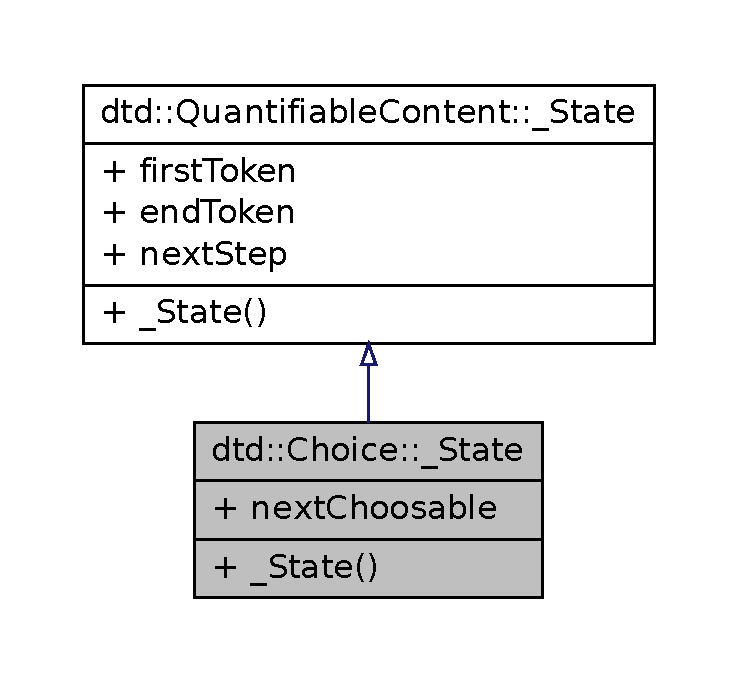
\includegraphics[width=354pt]{structdtd_1_1_choice_1_1___state__inherit__graph}
\end{center}
\end{figure}


Graphe de collaboration de dtd::Choice::\_\-State:\nopagebreak
\begin{figure}[H]
\begin{center}
\leavevmode
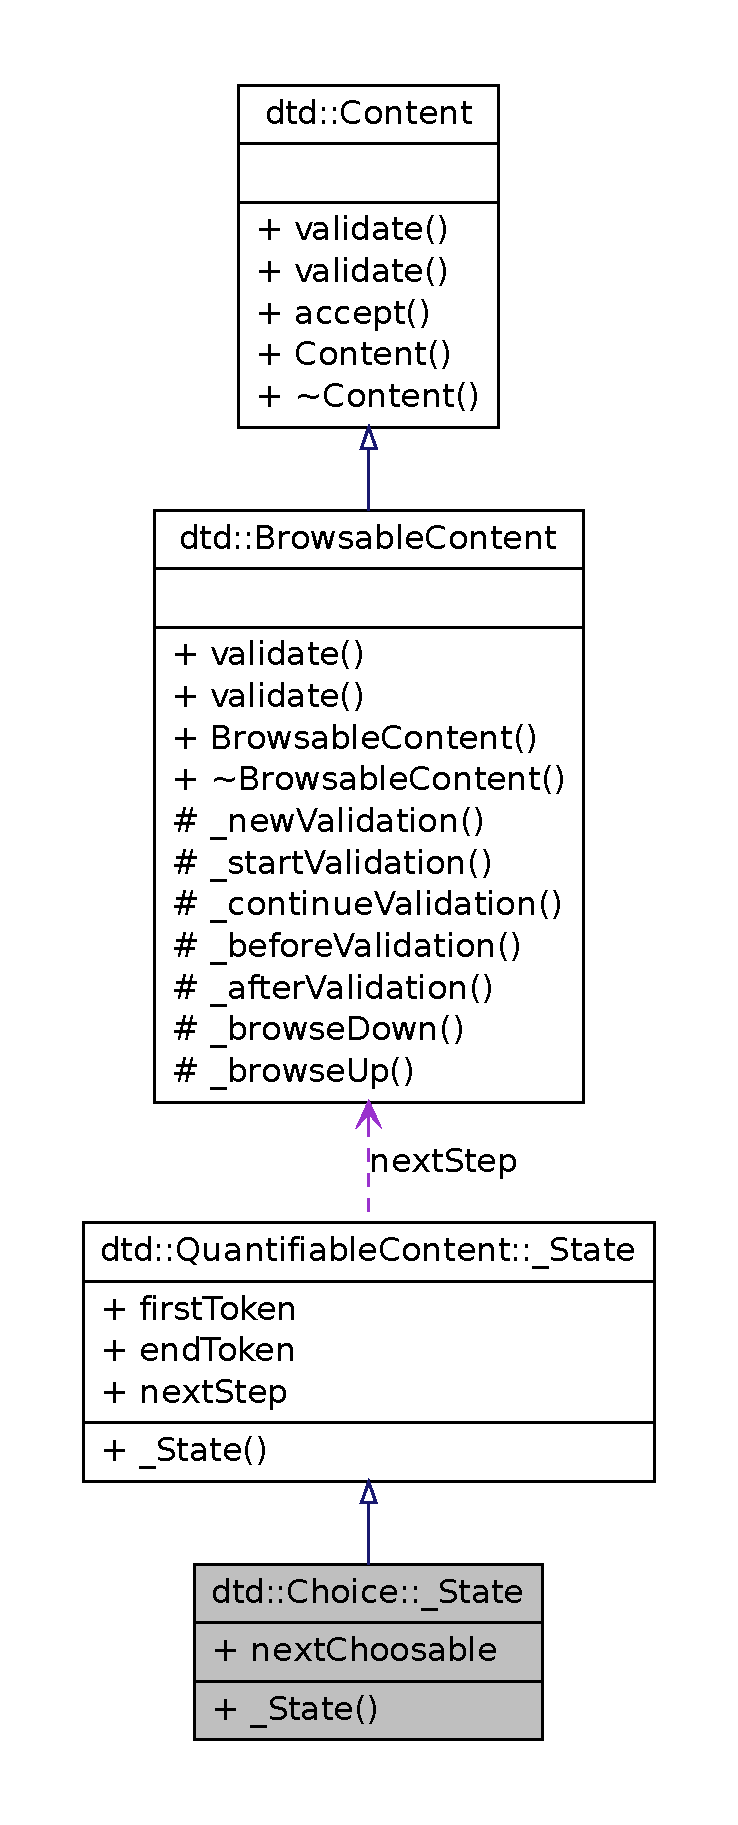
\includegraphics[height=600pt]{structdtd_1_1_choice_1_1___state__coll__graph}
\end{center}
\end{figure}
\subsection*{Fonctions membres publiques}
\begin{DoxyCompactItemize}
\item 
\hyperlink{structdtd_1_1_choice_1_1___state_a8c014d6674e17ef28429b38a535e20d6}{\_\-State} (xml::CompositeMarkupNode::ChildrenIterator aFirstToken, xml::CompositeMarkupNode::ChildrenIterator anEndToken, \hyperlink{classdtd_1_1_browsable_content}{BrowsableContent} $\ast$aNextStep, \_\-ChoosableSet::iterator aNextChoosable)
\end{DoxyCompactItemize}
\subsection*{Attributs publics}
\begin{DoxyCompactItemize}
\item 
\_\-ChoosableSet::iterator \hyperlink{structdtd_1_1_choice_1_1___state_a410e692510c4e6131c5a0f99fa36f4db}{nextChoosable}
\end{DoxyCompactItemize}


\subsection{Description détaillée}


Définition à la ligne 78 du fichier Choice.hh.



\subsection{Documentation des constructeurs et destructeur}
\hypertarget{structdtd_1_1_choice_1_1___state_a8c014d6674e17ef28429b38a535e20d6}{
\index{dtd::Choice::\_\-State@{dtd::Choice::\_\-State}!\_\-State@{\_\-State}}
\index{\_\-State@{\_\-State}!dtd::Choice::_State@{dtd::Choice::\_\-State}}
\subsubsection[{\_\-State}]{\setlength{\rightskip}{0pt plus 5cm}dtd::Choice::\_\-State::\_\-State (
\begin{DoxyParamCaption}
\item[{xml::CompositeMarkupNode::ChildrenIterator}]{ aFirstToken, }
\item[{xml::CompositeMarkupNode::ChildrenIterator}]{ anEndToken, }
\item[{{\bf BrowsableContent} $\ast$}]{ aNextStep, }
\item[{\_\-ChoosableSet::iterator}]{ aNextChoosable}
\end{DoxyParamCaption}
)\hspace{0.3cm}{\ttfamily  \mbox{[}inline\mbox{]}}}}
\label{structdtd_1_1_choice_1_1___state_a8c014d6674e17ef28429b38a535e20d6}


Définition à la ligne 82 du fichier Choice.hh.



\subsection{Documentation des données membres}
\hypertarget{structdtd_1_1_choice_1_1___state_a410e692510c4e6131c5a0f99fa36f4db}{
\index{dtd::Choice::\_\-State@{dtd::Choice::\_\-State}!nextChoosable@{nextChoosable}}
\index{nextChoosable@{nextChoosable}!dtd::Choice::_State@{dtd::Choice::\_\-State}}
\subsubsection[{nextChoosable}]{\setlength{\rightskip}{0pt plus 5cm}\_\-ChoosableSet::iterator {\bf dtd::Choice::\_\-State::nextChoosable}}}
\label{structdtd_1_1_choice_1_1___state_a410e692510c4e6131c5a0f99fa36f4db}


Définition à la ligne 80 du fichier Choice.hh.



La documentation de cette structure a été générée à partir du fichier suivant :\begin{DoxyCompactItemize}
\item 
src/\hyperlink{_choice_8hh}{Choice.hh}\end{DoxyCompactItemize}

\hypertarget{structdtd_1_1_quantifiable_content_1_1___state}{
\section{Référence de la structure dtd::QuantifiableContent::\_\-State}
\label{structdtd_1_1_quantifiable_content_1_1___state}\index{dtd::QuantifiableContent::\_\-State@{dtd::QuantifiableContent::\_\-State}}
}


{\ttfamily \#include $<$QuantifiableContent.hh$>$}



Graphe d'héritage de dtd::QuantifiableContent::\_\-State:\nopagebreak
\begin{figure}[H]
\begin{center}
\leavevmode
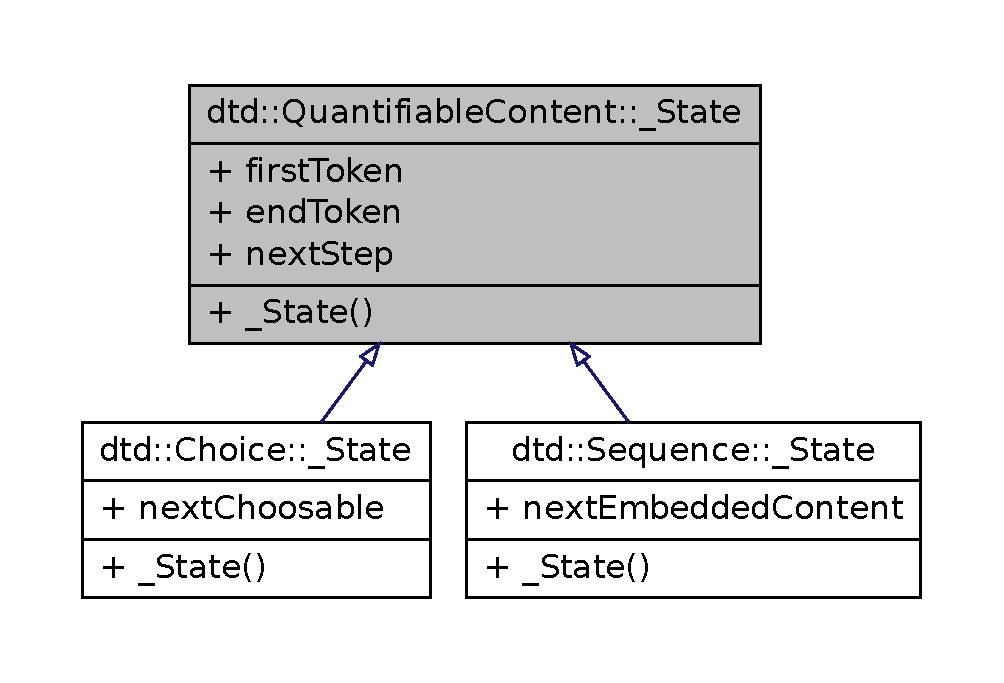
\includegraphics[width=400pt]{structdtd_1_1_quantifiable_content_1_1___state__inherit__graph}
\end{center}
\end{figure}


Graphe de collaboration de dtd::QuantifiableContent::\_\-State:\nopagebreak
\begin{figure}[H]
\begin{center}
\leavevmode
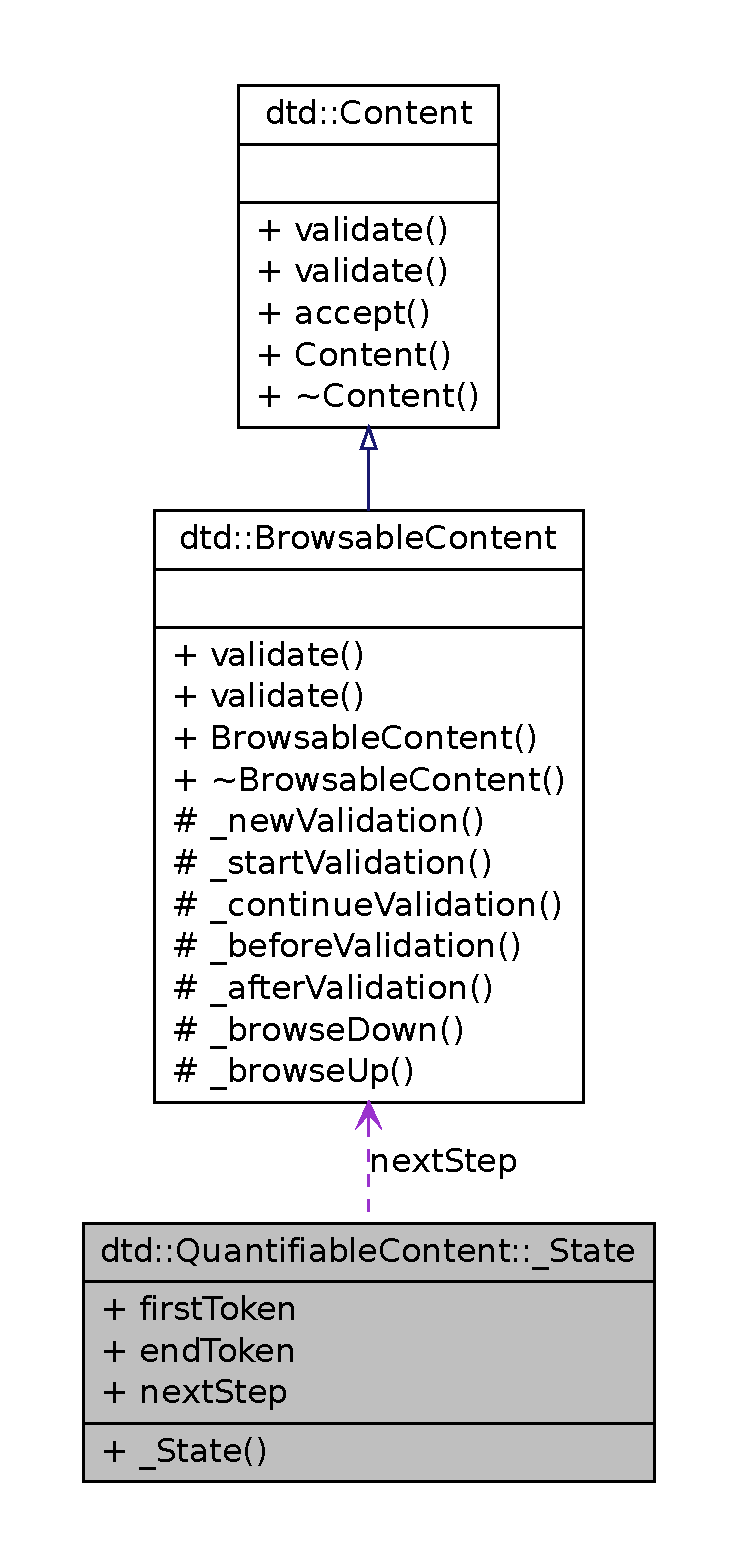
\includegraphics[height=600pt]{structdtd_1_1_quantifiable_content_1_1___state__coll__graph}
\end{center}
\end{figure}
\subsection*{Fonctions membres publiques}
\begin{DoxyCompactItemize}
\item 
\hyperlink{structdtd_1_1_quantifiable_content_1_1___state_a96e685e2095dcc538e3f190f73b0efcf}{\_\-State} (xml::CompositeMarkupNode::ChildrenIterator aFirstToken, xml::CompositeMarkupNode::ChildrenIterator anEndToken, \hyperlink{classdtd_1_1_browsable_content}{BrowsableContent} $\ast$aNextStep)
\end{DoxyCompactItemize}
\subsection*{Attributs publics}
\begin{DoxyCompactItemize}
\item 
xml::CompositeMarkupNode::ChildrenIterator \hyperlink{structdtd_1_1_quantifiable_content_1_1___state_a0d1bdfb22956d9f0f8a3b9c474660d11}{firstToken}
\item 
xml::CompositeMarkupNode::ChildrenIterator \hyperlink{structdtd_1_1_quantifiable_content_1_1___state_a926d0bb0e8f3a582834cf057be23d79f}{endToken}
\item 
\hyperlink{classdtd_1_1_browsable_content}{BrowsableContent} $\ast$ \hyperlink{structdtd_1_1_quantifiable_content_1_1___state_aab28474ad81a306c6ec1a450f941089b}{nextStep}
\end{DoxyCompactItemize}


\subsection{Description détaillée}


Définition à la ligne 50 du fichier QuantifiableContent.hh.



\subsection{Documentation des constructeurs et destructeur}
\hypertarget{structdtd_1_1_quantifiable_content_1_1___state_a96e685e2095dcc538e3f190f73b0efcf}{
\index{dtd::QuantifiableContent::\_\-State@{dtd::QuantifiableContent::\_\-State}!\_\-State@{\_\-State}}
\index{\_\-State@{\_\-State}!dtd::QuantifiableContent::_State@{dtd::QuantifiableContent::\_\-State}}
\subsubsection[{\_\-State}]{\setlength{\rightskip}{0pt plus 5cm}dtd::QuantifiableContent::\_\-State::\_\-State (
\begin{DoxyParamCaption}
\item[{xml::CompositeMarkupNode::ChildrenIterator}]{ aFirstToken, }
\item[{xml::CompositeMarkupNode::ChildrenIterator}]{ anEndToken, }
\item[{{\bf BrowsableContent} $\ast$}]{ aNextStep}
\end{DoxyParamCaption}
)\hspace{0.3cm}{\ttfamily  \mbox{[}inline\mbox{]}}}}
\label{structdtd_1_1_quantifiable_content_1_1___state_a96e685e2095dcc538e3f190f73b0efcf}


Définition à la ligne 56 du fichier QuantifiableContent.hh.



\subsection{Documentation des données membres}
\hypertarget{structdtd_1_1_quantifiable_content_1_1___state_a926d0bb0e8f3a582834cf057be23d79f}{
\index{dtd::QuantifiableContent::\_\-State@{dtd::QuantifiableContent::\_\-State}!endToken@{endToken}}
\index{endToken@{endToken}!dtd::QuantifiableContent::_State@{dtd::QuantifiableContent::\_\-State}}
\subsubsection[{endToken}]{\setlength{\rightskip}{0pt plus 5cm}xml::CompositeMarkupNode::ChildrenIterator {\bf dtd::QuantifiableContent::\_\-State::endToken}}}
\label{structdtd_1_1_quantifiable_content_1_1___state_a926d0bb0e8f3a582834cf057be23d79f}


Définition à la ligne 53 du fichier QuantifiableContent.hh.

\hypertarget{structdtd_1_1_quantifiable_content_1_1___state_a0d1bdfb22956d9f0f8a3b9c474660d11}{
\index{dtd::QuantifiableContent::\_\-State@{dtd::QuantifiableContent::\_\-State}!firstToken@{firstToken}}
\index{firstToken@{firstToken}!dtd::QuantifiableContent::_State@{dtd::QuantifiableContent::\_\-State}}
\subsubsection[{firstToken}]{\setlength{\rightskip}{0pt plus 5cm}xml::CompositeMarkupNode::ChildrenIterator {\bf dtd::QuantifiableContent::\_\-State::firstToken}}}
\label{structdtd_1_1_quantifiable_content_1_1___state_a0d1bdfb22956d9f0f8a3b9c474660d11}


Définition à la ligne 52 du fichier QuantifiableContent.hh.

\hypertarget{structdtd_1_1_quantifiable_content_1_1___state_aab28474ad81a306c6ec1a450f941089b}{
\index{dtd::QuantifiableContent::\_\-State@{dtd::QuantifiableContent::\_\-State}!nextStep@{nextStep}}
\index{nextStep@{nextStep}!dtd::QuantifiableContent::_State@{dtd::QuantifiableContent::\_\-State}}
\subsubsection[{nextStep}]{\setlength{\rightskip}{0pt plus 5cm}{\bf BrowsableContent}$\ast$ {\bf dtd::QuantifiableContent::\_\-State::nextStep}}}
\label{structdtd_1_1_quantifiable_content_1_1___state_aab28474ad81a306c6ec1a450f941089b}


Définition à la ligne 54 du fichier QuantifiableContent.hh.



La documentation de cette structure a été générée à partir du fichier suivant :\begin{DoxyCompactItemize}
\item 
src/\hyperlink{_quantifiable_content_8hh}{QuantifiableContent.hh}\end{DoxyCompactItemize}

\hypertarget{structdtd_1_1_sequence_1_1___state}{
\section{Référence de la structure dtd::Sequence::\_\-State}
\label{structdtd_1_1_sequence_1_1___state}\index{dtd::Sequence::\_\-State@{dtd::Sequence::\_\-State}}
}


{\ttfamily \#include $<$Sequence.hh$>$}



Graphe d'héritage de dtd::Sequence::\_\-State:\nopagebreak
\begin{figure}[H]
\begin{center}
\leavevmode
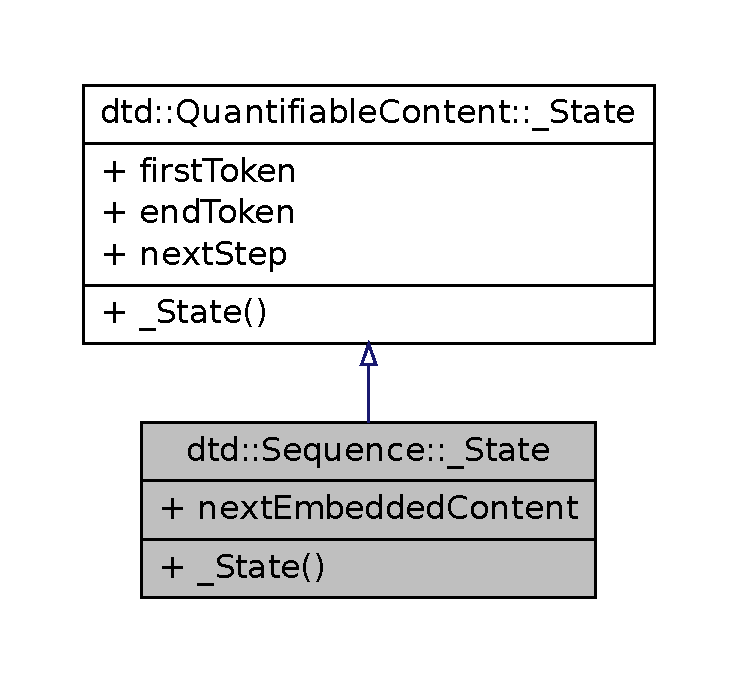
\includegraphics[width=354pt]{structdtd_1_1_sequence_1_1___state__inherit__graph}
\end{center}
\end{figure}


Graphe de collaboration de dtd::Sequence::\_\-State:\nopagebreak
\begin{figure}[H]
\begin{center}
\leavevmode
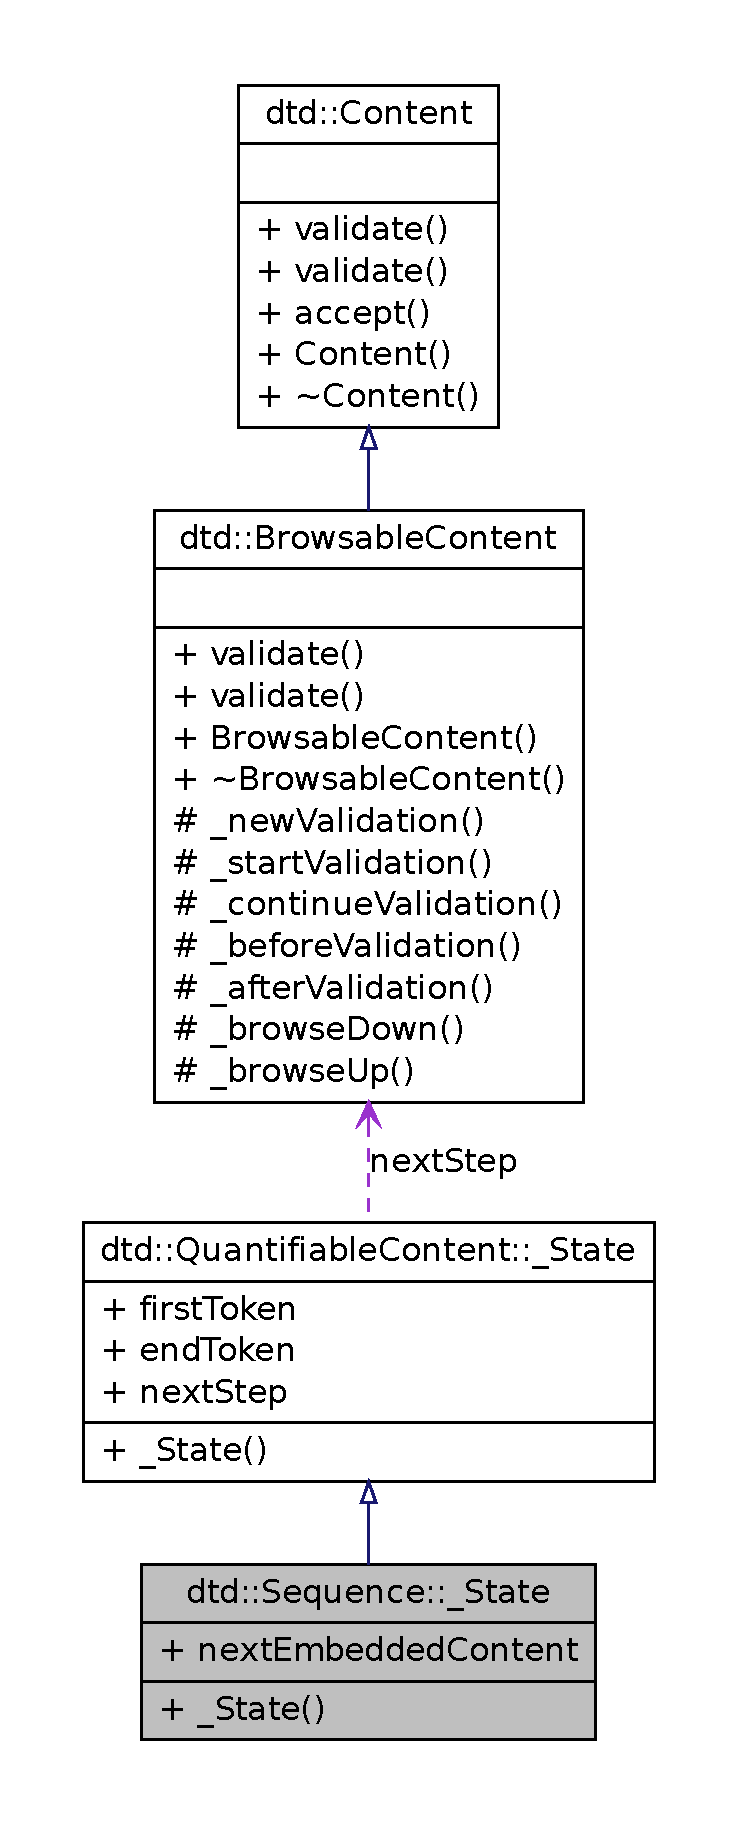
\includegraphics[height=600pt]{structdtd_1_1_sequence_1_1___state__coll__graph}
\end{center}
\end{figure}
\subsection*{Fonctions membres publiques}
\begin{DoxyCompactItemize}
\item 
\hyperlink{structdtd_1_1_sequence_1_1___state_af1e1d0084dedb7c9b1bf8ea0e2e3b787}{\_\-State} (xml::CompositeMarkupNode::ChildrenIterator aFirstToken, xml::CompositeMarkupNode::ChildrenIterator anEndToken, \hyperlink{classdtd_1_1_browsable_content}{BrowsableContent} $\ast$aNextStep, \_\-OrderedContent::iterator aNextEmbeddedContent)
\end{DoxyCompactItemize}
\subsection*{Attributs publics}
\begin{DoxyCompactItemize}
\item 
\_\-OrderedContent::iterator \hyperlink{structdtd_1_1_sequence_1_1___state_add6dbb226fdf04d4c5d8250add9028f7}{nextEmbeddedContent}
\end{DoxyCompactItemize}


\subsection{Description détaillée}


Définition à la ligne 83 du fichier Sequence.hh.



\subsection{Documentation des constructeurs et destructeur}
\hypertarget{structdtd_1_1_sequence_1_1___state_af1e1d0084dedb7c9b1bf8ea0e2e3b787}{
\index{dtd::Sequence::\_\-State@{dtd::Sequence::\_\-State}!\_\-State@{\_\-State}}
\index{\_\-State@{\_\-State}!dtd::Sequence::_State@{dtd::Sequence::\_\-State}}
\subsubsection[{\_\-State}]{\setlength{\rightskip}{0pt plus 5cm}dtd::Sequence::\_\-State::\_\-State (
\begin{DoxyParamCaption}
\item[{xml::CompositeMarkupNode::ChildrenIterator}]{ aFirstToken, }
\item[{xml::CompositeMarkupNode::ChildrenIterator}]{ anEndToken, }
\item[{{\bf BrowsableContent} $\ast$}]{ aNextStep, }
\item[{\_\-OrderedContent::iterator}]{ aNextEmbeddedContent}
\end{DoxyParamCaption}
)\hspace{0.3cm}{\ttfamily  \mbox{[}inline\mbox{]}}}}
\label{structdtd_1_1_sequence_1_1___state_af1e1d0084dedb7c9b1bf8ea0e2e3b787}


Définition à la ligne 87 du fichier Sequence.hh.



\subsection{Documentation des données membres}
\hypertarget{structdtd_1_1_sequence_1_1___state_add6dbb226fdf04d4c5d8250add9028f7}{
\index{dtd::Sequence::\_\-State@{dtd::Sequence::\_\-State}!nextEmbeddedContent@{nextEmbeddedContent}}
\index{nextEmbeddedContent@{nextEmbeddedContent}!dtd::Sequence::_State@{dtd::Sequence::\_\-State}}
\subsubsection[{nextEmbeddedContent}]{\setlength{\rightskip}{0pt plus 5cm}\_\-OrderedContent::iterator {\bf dtd::Sequence::\_\-State::nextEmbeddedContent}}}
\label{structdtd_1_1_sequence_1_1___state_add6dbb226fdf04d4c5d8250add9028f7}


Définition à la ligne 85 du fichier Sequence.hh.



La documentation de cette structure a été générée à partir du fichier suivant :\begin{DoxyCompactItemize}
\item 
src/\hyperlink{_sequence_8hh}{Sequence.hh}\end{DoxyCompactItemize}

\hypertarget{classdtd_1_1_any_content}{
\section{Référence de la classe dtd::AnyContent}
\label{classdtd_1_1_any_content}\index{dtd::AnyContent@{dtd::AnyContent}}
}


{\ttfamily \#include $<$AnyContent.hh$>$}



Graphe d'héritage de dtd::AnyContent:\nopagebreak
\begin{figure}[H]
\begin{center}
\leavevmode
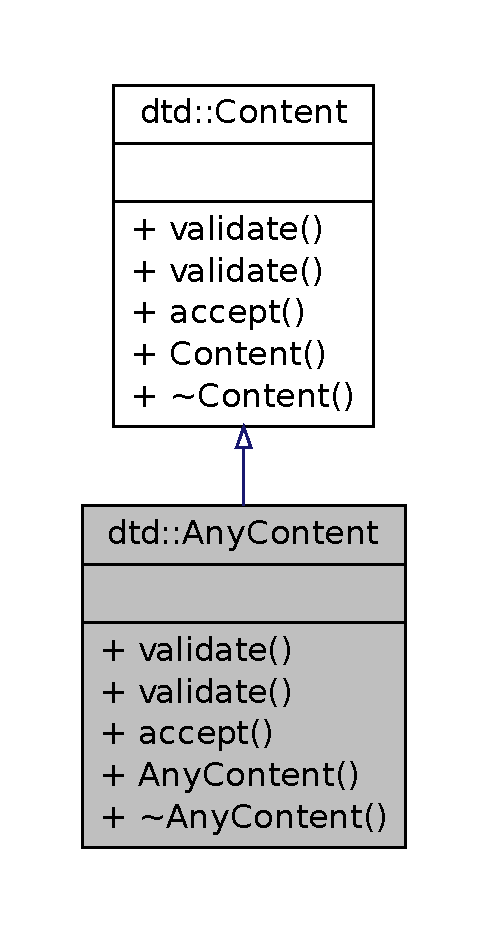
\includegraphics[width=234pt]{classdtd_1_1_any_content__inherit__graph}
\end{center}
\end{figure}


Graphe de collaboration de dtd::AnyContent:\nopagebreak
\begin{figure}[H]
\begin{center}
\leavevmode
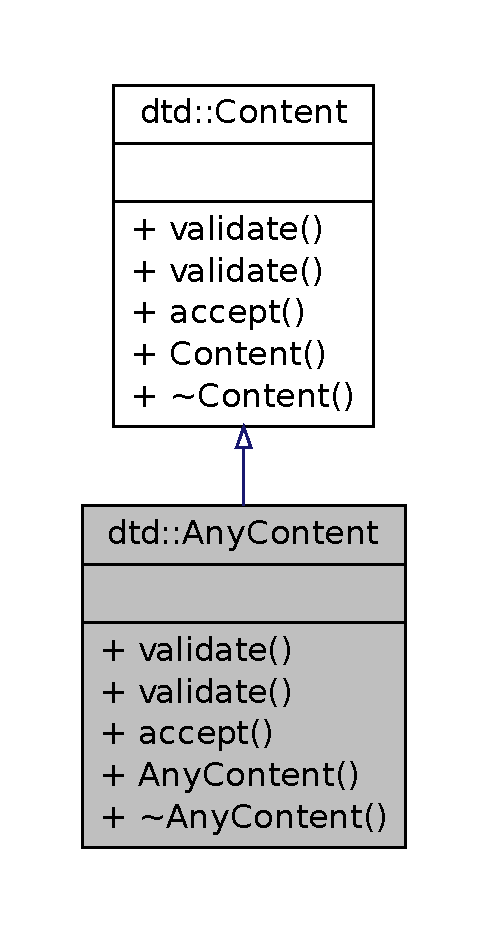
\includegraphics[width=234pt]{classdtd_1_1_any_content__coll__graph}
\end{center}
\end{figure}
\subsection*{Fonctions membres publiques}
\begin{DoxyCompactItemize}
\item 
virtual bool \hyperlink{classdtd_1_1_any_content_a1c69a5e152cec9428a72b83e1a86da67}{validate} (const xml::MarkupNode \&node)
\item 
virtual bool \hyperlink{classdtd_1_1_any_content_a6bd017d55e1c6eb09bdb7944afe57ab2}{validate} (const xml::CompositeMarkupNode \&node)
\item 
virtual void \hyperlink{classdtd_1_1_any_content_ae9e5cecd79f91449de424a24944295cf}{accept} (\hyperlink{classdtd_1_1_interface_d_t_d_visitor}{InterfaceDTDVisitor} \&visitor) const 
\item 
\hyperlink{classdtd_1_1_any_content_a1747b428c9253e03e9926d777dc577bc}{AnyContent} ()
\item 
virtual \hyperlink{classdtd_1_1_any_content_a30639c2b4d84eab8288d81e61ae4ba2a}{$\sim$AnyContent} ()
\end{DoxyCompactItemize}


\subsection{Description détaillée}


Définition à la ligne 18 du fichier AnyContent.hh.



\subsection{Documentation des constructeurs et destructeur}
\hypertarget{classdtd_1_1_any_content_a1747b428c9253e03e9926d777dc577bc}{
\index{dtd::AnyContent@{dtd::AnyContent}!AnyContent@{AnyContent}}
\index{AnyContent@{AnyContent}!dtd::AnyContent@{dtd::AnyContent}}
\subsubsection[{AnyContent}]{\setlength{\rightskip}{0pt plus 5cm}dtd::AnyContent::AnyContent (
\begin{DoxyParamCaption}
{}
\end{DoxyParamCaption}
)}}
\label{classdtd_1_1_any_content_a1747b428c9253e03e9926d777dc577bc}


Définition à la ligne 52 du fichier AnyContent.cpp.

\hypertarget{classdtd_1_1_any_content_a30639c2b4d84eab8288d81e61ae4ba2a}{
\index{dtd::AnyContent@{dtd::AnyContent}!$\sim$AnyContent@{$\sim$AnyContent}}
\index{$\sim$AnyContent@{$\sim$AnyContent}!dtd::AnyContent@{dtd::AnyContent}}
\subsubsection[{$\sim$AnyContent}]{\setlength{\rightskip}{0pt plus 5cm}dtd::AnyContent::$\sim$AnyContent (
\begin{DoxyParamCaption}
{}
\end{DoxyParamCaption}
)\hspace{0.3cm}{\ttfamily  \mbox{[}virtual\mbox{]}}}}
\label{classdtd_1_1_any_content_a30639c2b4d84eab8288d81e61ae4ba2a}


Définition à la ligne 57 du fichier AnyContent.cpp.



\subsection{Documentation des fonctions membres}
\hypertarget{classdtd_1_1_any_content_ae9e5cecd79f91449de424a24944295cf}{
\index{dtd::AnyContent@{dtd::AnyContent}!accept@{accept}}
\index{accept@{accept}!dtd::AnyContent@{dtd::AnyContent}}
\subsubsection[{accept}]{\setlength{\rightskip}{0pt plus 5cm}void dtd::AnyContent::accept (
\begin{DoxyParamCaption}
\item[{{\bf InterfaceDTDVisitor} \&}]{ visitor}
\end{DoxyParamCaption}
) const\hspace{0.3cm}{\ttfamily  \mbox{[}virtual\mbox{]}}}}
\label{classdtd_1_1_any_content_ae9e5cecd79f91449de424a24944295cf}


Implémente \hyperlink{classdtd_1_1_content_a403cc15f12eaa187ad493fa600540cd8}{dtd::Content}.



Définition à la ligne 43 du fichier AnyContent.cpp.



Voici le graphe d'appel pour cette fonction :\nopagebreak
\begin{figure}[H]
\begin{center}
\leavevmode
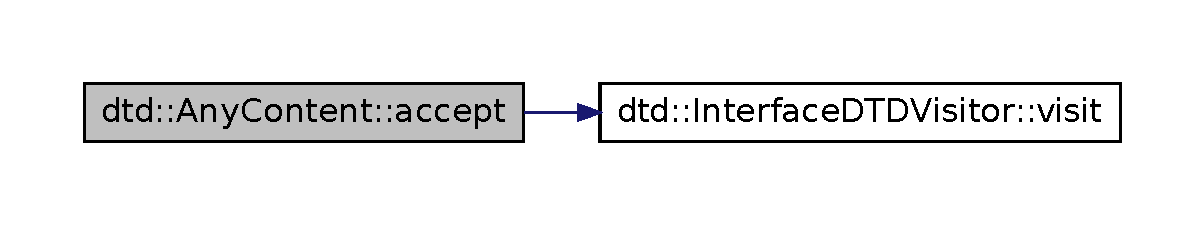
\includegraphics[width=400pt]{classdtd_1_1_any_content_ae9e5cecd79f91449de424a24944295cf_cgraph}
\end{center}
\end{figure}


\hypertarget{classdtd_1_1_any_content_a1c69a5e152cec9428a72b83e1a86da67}{
\index{dtd::AnyContent@{dtd::AnyContent}!validate@{validate}}
\index{validate@{validate}!dtd::AnyContent@{dtd::AnyContent}}
\subsubsection[{validate}]{\setlength{\rightskip}{0pt plus 5cm}virtual bool dtd::AnyContent::validate (
\begin{DoxyParamCaption}
\item[{const xml::MarkupNode \&}]{ node}
\end{DoxyParamCaption}
)\hspace{0.3cm}{\ttfamily  \mbox{[}virtual\mbox{]}}}}
\label{classdtd_1_1_any_content_a1c69a5e152cec9428a72b83e1a86da67}


Implémente \hyperlink{classdtd_1_1_content_a2095fb10a09f6767aaf5e6da4b3018f1}{dtd::Content}.

\hypertarget{classdtd_1_1_any_content_a6bd017d55e1c6eb09bdb7944afe57ab2}{
\index{dtd::AnyContent@{dtd::AnyContent}!validate@{validate}}
\index{validate@{validate}!dtd::AnyContent@{dtd::AnyContent}}
\subsubsection[{validate}]{\setlength{\rightskip}{0pt plus 5cm}virtual bool dtd::AnyContent::validate (
\begin{DoxyParamCaption}
\item[{const xml::CompositeMarkupNode \&}]{ node}
\end{DoxyParamCaption}
)\hspace{0.3cm}{\ttfamily  \mbox{[}virtual\mbox{]}}}}
\label{classdtd_1_1_any_content_a6bd017d55e1c6eb09bdb7944afe57ab2}


Implémente \hyperlink{classdtd_1_1_content_acaa15daa3a3a2cf11632c4c93dc2cf37}{dtd::Content}.



La documentation de cette classe a été générée à partir des fichiers suivants :\begin{DoxyCompactItemize}
\item 
src/\hyperlink{_any_content_8hh}{AnyContent.hh}\item 
src/\hyperlink{_any_content_8cpp}{AnyContent.cpp}\end{DoxyCompactItemize}

\hypertarget{classdtd_1_1_attribute}{
\section{Référence de la classe dtd::Attribute}
\label{classdtd_1_1_attribute}\index{dtd::Attribute@{dtd::Attribute}}
}


{\ttfamily \#include $<$Attribute.hh$>$}

\subsection*{Fonctions membres publiques}
\begin{DoxyCompactItemize}
\item 
std::string \hyperlink{classdtd_1_1_attribute_a3d1e42a5210df12eaccdb2b2d6ce6147}{name} () const 
\item 
\hyperlink{classdtd_1_1_attribute_a776a0717a54d9d071704f69118797f84}{Attribute} (const std::string \&name)
\item 
virtual \hyperlink{classdtd_1_1_attribute_a5bcf54eef0c5573abb39469bd76c2dd3}{$\sim$Attribute} ()
\end{DoxyCompactItemize}
\subsection*{Attributs protégés}
\begin{DoxyCompactItemize}
\item 
std::string \hyperlink{classdtd_1_1_attribute_a1df987474cc5fb17dd4ce699e50443c8}{\_\-name}
\end{DoxyCompactItemize}


\subsection{Description détaillée}


Définition à la ligne 18 du fichier Attribute.hh.



\subsection{Documentation des constructeurs et destructeur}
\hypertarget{classdtd_1_1_attribute_a776a0717a54d9d071704f69118797f84}{
\index{dtd::Attribute@{dtd::Attribute}!Attribute@{Attribute}}
\index{Attribute@{Attribute}!dtd::Attribute@{dtd::Attribute}}
\subsubsection[{Attribute}]{\setlength{\rightskip}{0pt plus 5cm}dtd::Attribute::Attribute (
\begin{DoxyParamCaption}
\item[{const std::string \&}]{ name}
\end{DoxyParamCaption}
)}}
\label{classdtd_1_1_attribute_a776a0717a54d9d071704f69118797f84}
\hypertarget{classdtd_1_1_attribute_a5bcf54eef0c5573abb39469bd76c2dd3}{
\index{dtd::Attribute@{dtd::Attribute}!$\sim$Attribute@{$\sim$Attribute}}
\index{$\sim$Attribute@{$\sim$Attribute}!dtd::Attribute@{dtd::Attribute}}
\subsubsection[{$\sim$Attribute}]{\setlength{\rightskip}{0pt plus 5cm}dtd::Attribute::$\sim$Attribute (
\begin{DoxyParamCaption}
{}
\end{DoxyParamCaption}
)\hspace{0.3cm}{\ttfamily  \mbox{[}virtual\mbox{]}}}}
\label{classdtd_1_1_attribute_a5bcf54eef0c5573abb39469bd76c2dd3}


Définition à la ligne 46 du fichier Attribute.cpp.



\subsection{Documentation des fonctions membres}
\hypertarget{classdtd_1_1_attribute_a3d1e42a5210df12eaccdb2b2d6ce6147}{
\index{dtd::Attribute@{dtd::Attribute}!name@{name}}
\index{name@{name}!dtd::Attribute@{dtd::Attribute}}
\subsubsection[{name}]{\setlength{\rightskip}{0pt plus 5cm}string dtd::Attribute::name (
\begin{DoxyParamCaption}
{}
\end{DoxyParamCaption}
) const}}
\label{classdtd_1_1_attribute_a3d1e42a5210df12eaccdb2b2d6ce6147}


Définition à la ligne 31 du fichier Attribute.cpp.



Voici le graphe d'appel pour cette fonction :\nopagebreak
\begin{figure}[H]
\begin{center}
\leavevmode
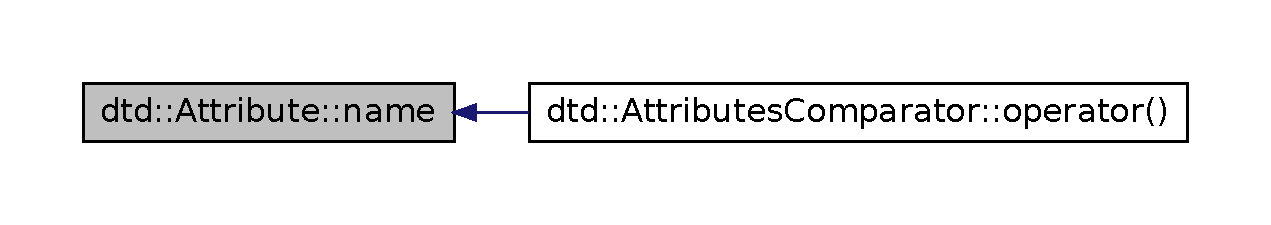
\includegraphics[width=400pt]{classdtd_1_1_attribute_a3d1e42a5210df12eaccdb2b2d6ce6147_icgraph}
\end{center}
\end{figure}




\subsection{Documentation des données membres}
\hypertarget{classdtd_1_1_attribute_a1df987474cc5fb17dd4ce699e50443c8}{
\index{dtd::Attribute@{dtd::Attribute}!\_\-name@{\_\-name}}
\index{\_\-name@{\_\-name}!dtd::Attribute@{dtd::Attribute}}
\subsubsection[{\_\-name}]{\setlength{\rightskip}{0pt plus 5cm}std::string {\bf dtd::Attribute::\_\-name}\hspace{0.3cm}{\ttfamily  \mbox{[}protected\mbox{]}}}}
\label{classdtd_1_1_attribute_a1df987474cc5fb17dd4ce699e50443c8}


Définition à la ligne 43 du fichier Attribute.hh.



La documentation de cette classe a été générée à partir des fichiers suivants :\begin{DoxyCompactItemize}
\item 
src/\hyperlink{_attribute_8hh}{Attribute.hh}\item 
src/\hyperlink{_attribute_8cpp}{Attribute.cpp}\end{DoxyCompactItemize}

\hypertarget{structdtd_1_1_attributes_comparator}{
\section{Référence de la structure dtd::AttributesComparator}
\label{structdtd_1_1_attributes_comparator}\index{dtd::AttributesComparator@{dtd::AttributesComparator}}
}


{\ttfamily \#include $<$AttributesList.hh$>$}

\subsection*{Fonctions membres publiques}
\begin{DoxyCompactItemize}
\item 
bool \hyperlink{structdtd_1_1_attributes_comparator_abfedc16b191edd3b2acd4cfc5522417b}{operator()} (const \hyperlink{classdtd_1_1_attribute}{Attribute} $\ast$const \&x, const \hyperlink{classdtd_1_1_attribute}{Attribute} $\ast$const \&y) const 
\end{DoxyCompactItemize}


\subsection{Description détaillée}


Définition à la ligne 20 du fichier AttributesList.hh.



\subsection{Documentation des fonctions membres}
\hypertarget{structdtd_1_1_attributes_comparator_abfedc16b191edd3b2acd4cfc5522417b}{
\index{dtd::AttributesComparator@{dtd::AttributesComparator}!operator()@{operator()}}
\index{operator()@{operator()}!dtd::AttributesComparator@{dtd::AttributesComparator}}
\subsubsection[{operator()}]{\setlength{\rightskip}{0pt plus 5cm}bool dtd::AttributesComparator::operator() (
\begin{DoxyParamCaption}
\item[{const {\bf Attribute} $\ast$const \&}]{ x, }
\item[{const {\bf Attribute} $\ast$const \&}]{ y}
\end{DoxyParamCaption}
) const\hspace{0.3cm}{\ttfamily  \mbox{[}inline\mbox{]}}}}
\label{structdtd_1_1_attributes_comparator_abfedc16b191edd3b2acd4cfc5522417b}


Définition à la ligne 22 du fichier AttributesList.hh.



Voici le graphe d'appel pour cette fonction :\nopagebreak
\begin{figure}[H]
\begin{center}
\leavevmode
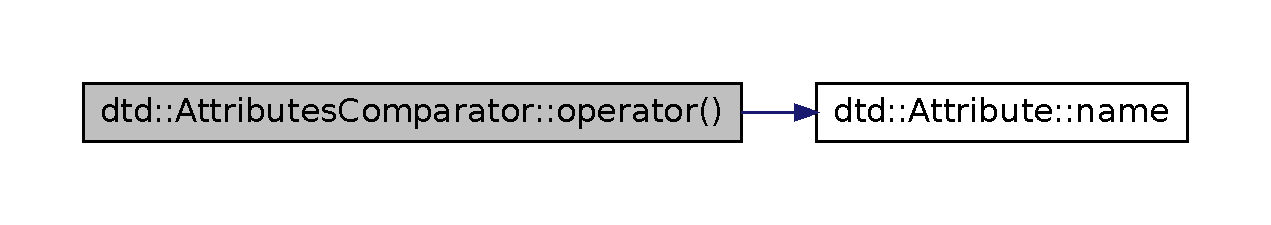
\includegraphics[width=400pt]{structdtd_1_1_attributes_comparator_abfedc16b191edd3b2acd4cfc5522417b_cgraph}
\end{center}
\end{figure}




La documentation de cette structure a été générée à partir du fichier suivant :\begin{DoxyCompactItemize}
\item 
src/\hyperlink{_attributes_list_8hh}{AttributesList.hh}\end{DoxyCompactItemize}

\hypertarget{classdtd_1_1_browsable_content}{
\section{Référence de la classe dtd::BrowsableContent}
\label{classdtd_1_1_browsable_content}\index{dtd::BrowsableContent@{dtd::BrowsableContent}}
}


{\ttfamily \#include $<$BrowsableContent.hh$>$}



Graphe d'héritage de dtd::BrowsableContent:\nopagebreak
\begin{figure}[H]
\begin{center}
\leavevmode
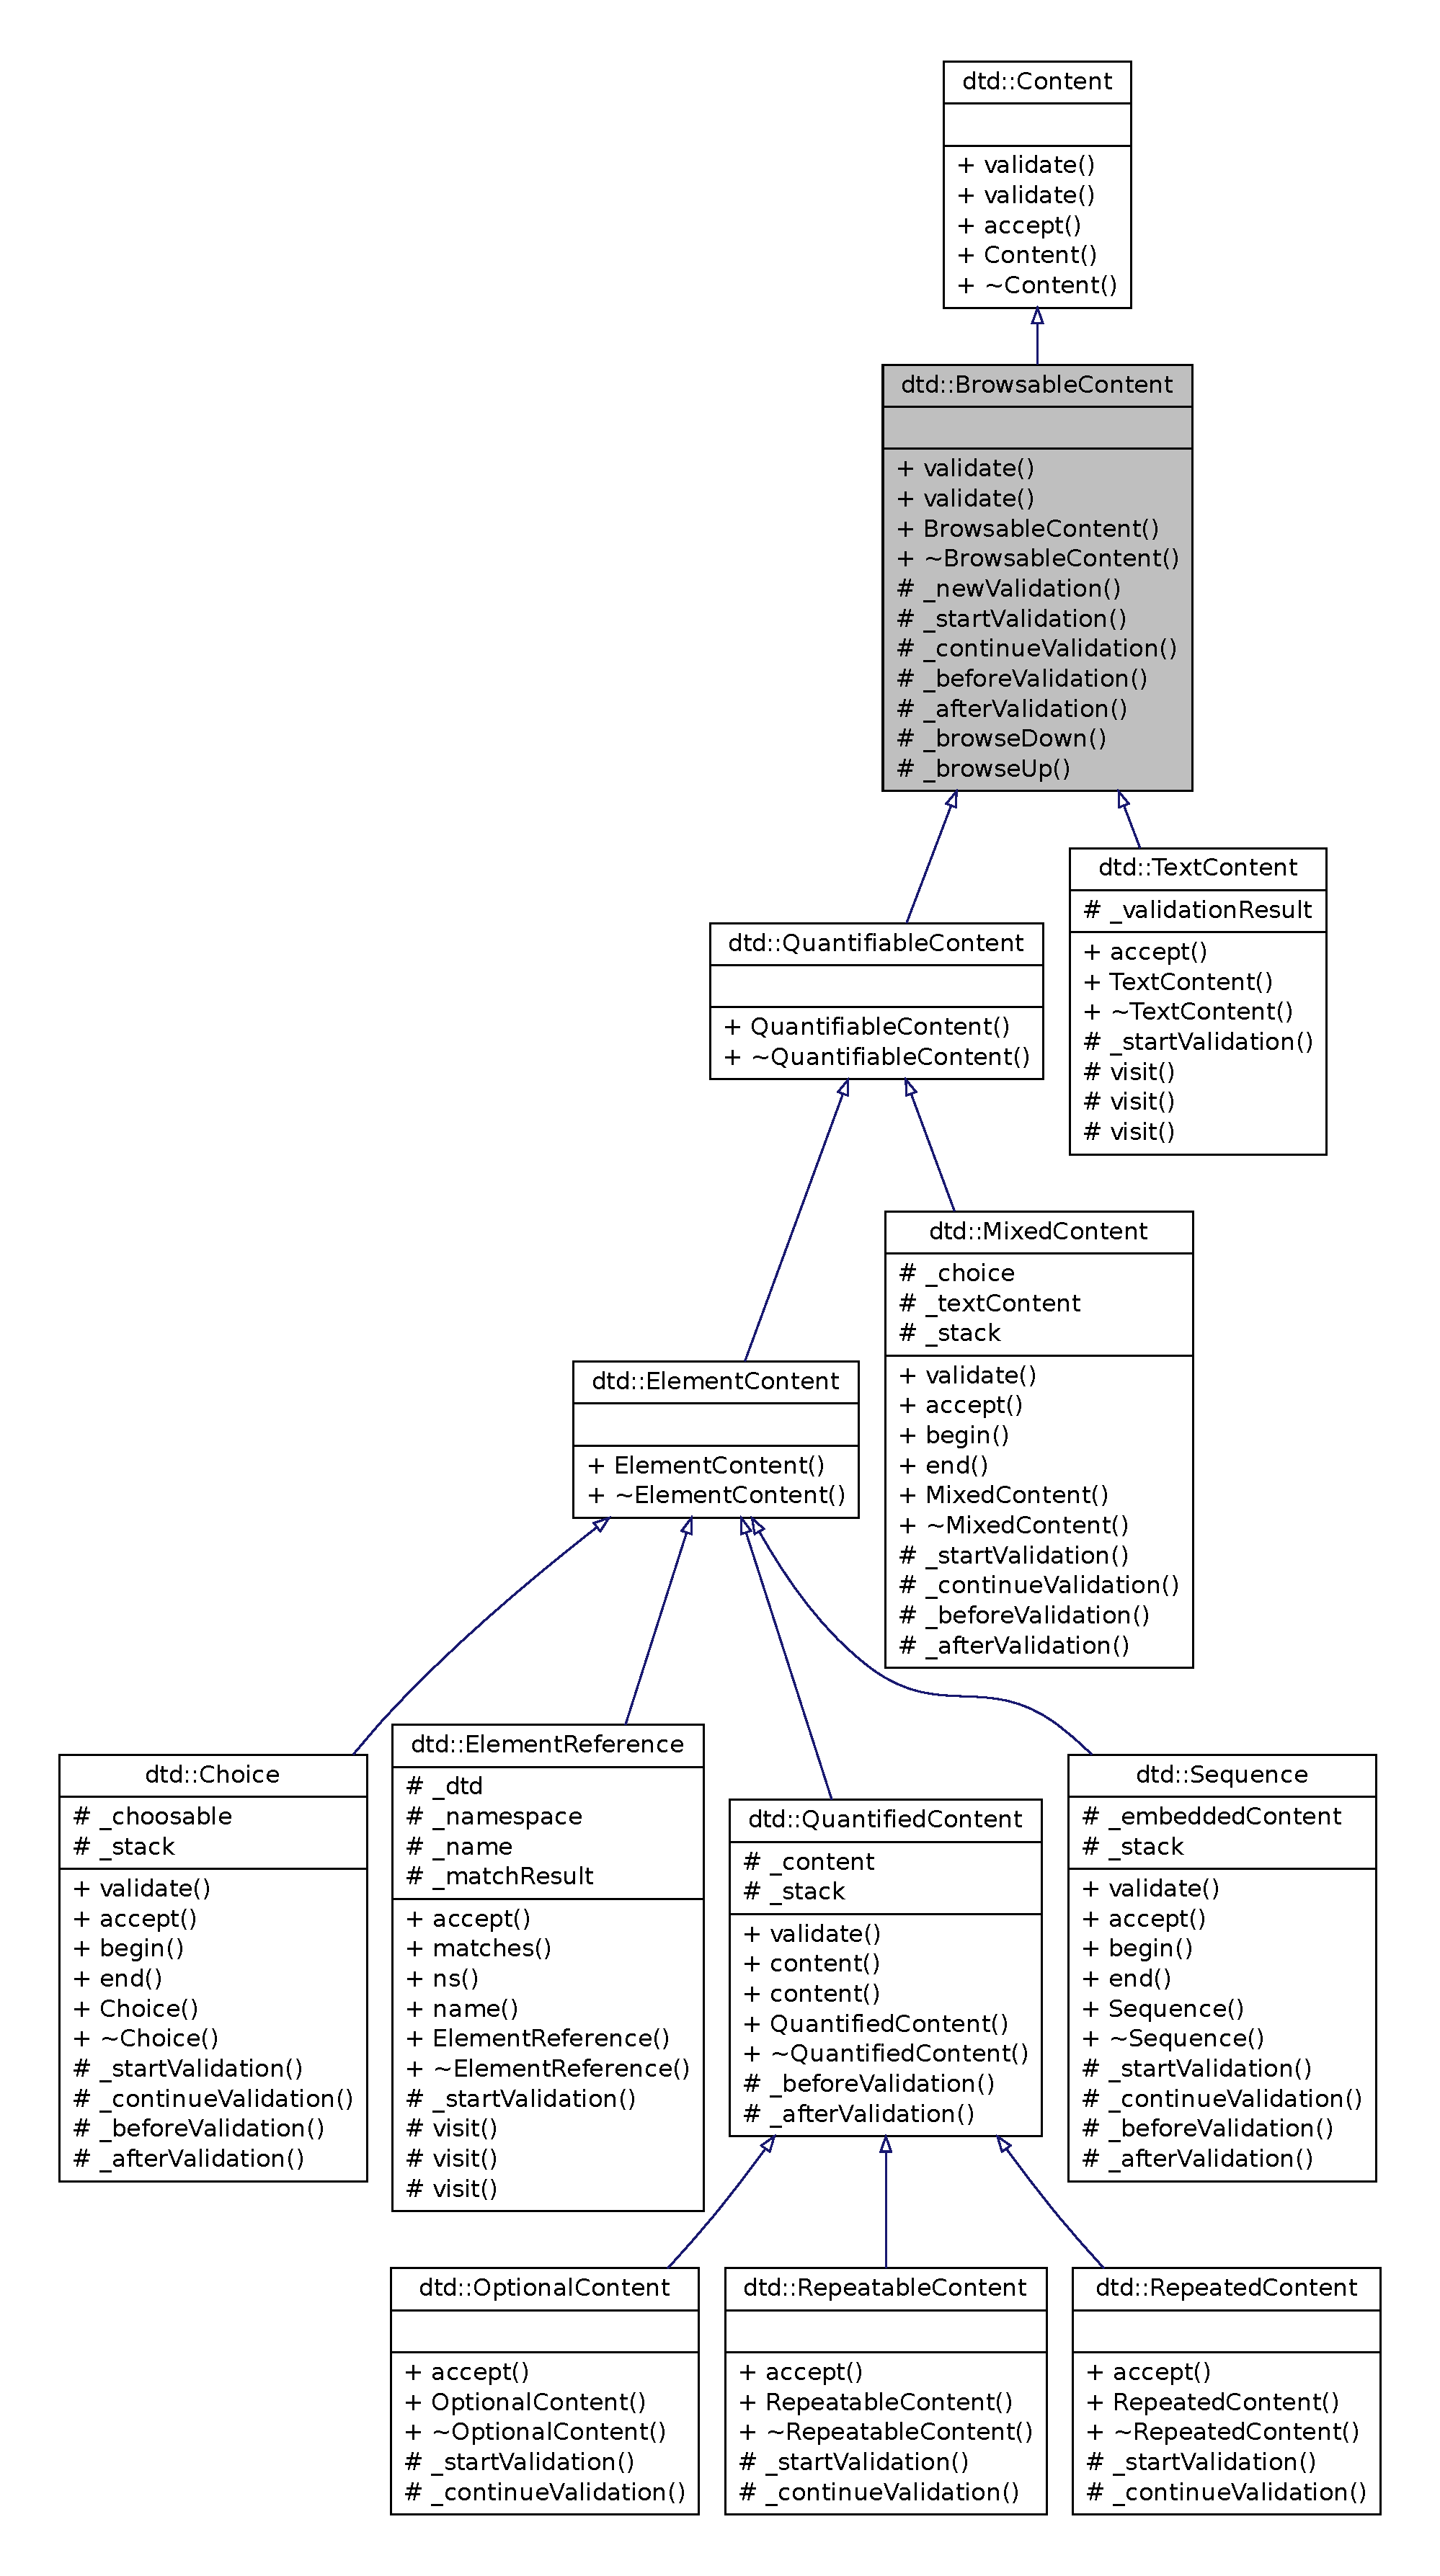
\includegraphics[height=600pt]{classdtd_1_1_browsable_content__inherit__graph}
\end{center}
\end{figure}


Graphe de collaboration de dtd::BrowsableContent:\nopagebreak
\begin{figure}[H]
\begin{center}
\leavevmode
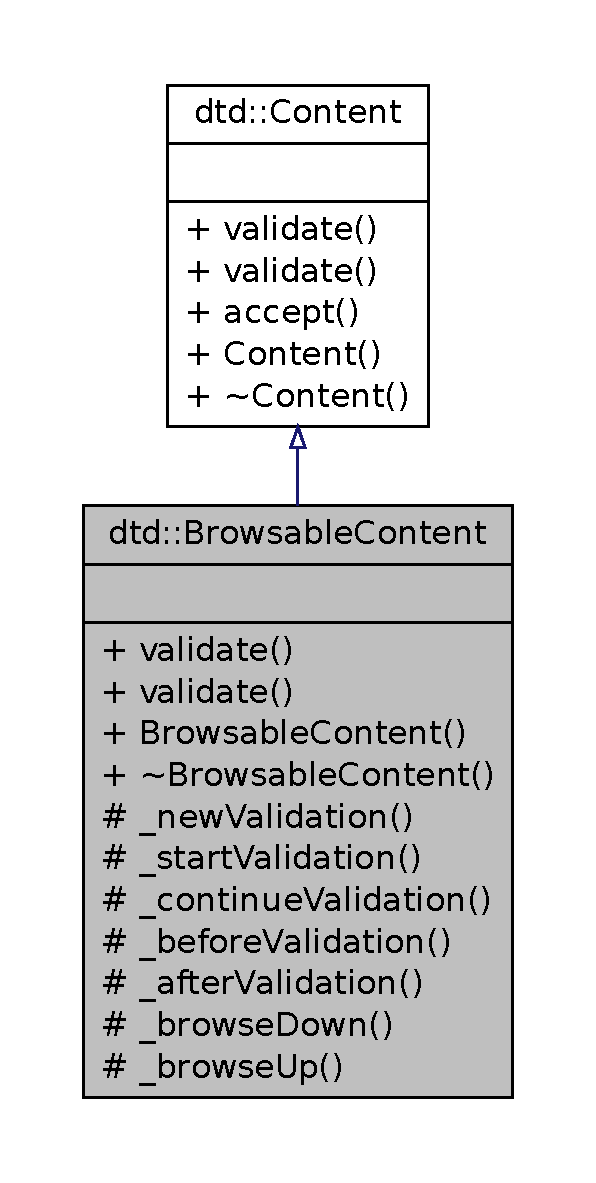
\includegraphics[width=286pt]{classdtd_1_1_browsable_content__coll__graph}
\end{center}
\end{figure}
\subsection*{Fonctions membres publiques}
\begin{DoxyCompactItemize}
\item 
virtual bool \hyperlink{classdtd_1_1_browsable_content_adbd9d013e126d5a1b601c3d781181bd4}{validate} (const xml::MarkupNode \&node)
\item 
virtual bool \hyperlink{classdtd_1_1_browsable_content_a824a0c41b66aeea689e4283ee453d398}{validate} (const xml::CompositeMarkupNode \&node)
\item 
\hyperlink{classdtd_1_1_browsable_content_a1f08c9ba0fa256b18ddbf473f3d7a868}{BrowsableContent} ()
\item 
virtual \hyperlink{classdtd_1_1_browsable_content_a0ccac4ea5cfbaf919b4a51b7b8537d0c}{$\sim$BrowsableContent} ()
\end{DoxyCompactItemize}
\subsection*{Fonctions membres protégées}
\begin{DoxyCompactItemize}
\item 
bool \hyperlink{classdtd_1_1_browsable_content_a54a43ef27f874748f99b8ab71c23e2dc}{\_\-newValidation} (xml::CompositeMarkupNode::ChildrenIterator firstToken, xml::CompositeMarkupNode::ChildrenIterator endToken, \hyperlink{classdtd_1_1_browsable_content}{BrowsableContent} $\ast$nextStep)
\item 
virtual bool \hyperlink{classdtd_1_1_browsable_content_a67ab5a7329d94e363796ae2d17617246}{\_\-startValidation} (xml::CompositeMarkupNode::ChildrenIterator firstToken, xml::CompositeMarkupNode::ChildrenIterator endToken, \hyperlink{classdtd_1_1_browsable_content}{BrowsableContent} $\ast$nextStep)=0
\item 
virtual bool \hyperlink{classdtd_1_1_browsable_content_a6398e5990648e2af3fd775592b0d62ea}{\_\-continueValidation} (xml::CompositeMarkupNode::ChildrenIterator currentToken)
\item 
virtual void \hyperlink{classdtd_1_1_browsable_content_ae9e55da18cc09557fc7896a7ccac2ee1}{\_\-beforeValidation} (xml::CompositeMarkupNode::ChildrenIterator firstToken, xml::CompositeMarkupNode::ChildrenIterator endToken, \hyperlink{classdtd_1_1_browsable_content}{BrowsableContent} $\ast$nextStep)
\item 
virtual void \hyperlink{classdtd_1_1_browsable_content_a378fc620af75eb9bad9f37c663e3838d}{\_\-afterValidation} ()
\item 
bool \hyperlink{classdtd_1_1_browsable_content_aea818259a913cb7359d902ee121c4e87}{\_\-browseDown} (\hyperlink{classdtd_1_1_browsable_content}{BrowsableContent} \&childContent, xml::CompositeMarkupNode::ChildrenIterator firstToken, xml::CompositeMarkupNode::ChildrenIterator endToken, \hyperlink{classdtd_1_1_browsable_content}{BrowsableContent} $\ast$nextStep)
\item 
bool \hyperlink{classdtd_1_1_browsable_content_a267660fa668e638d6487a875ffd958b0}{\_\-browseUp} (\hyperlink{classdtd_1_1_browsable_content}{BrowsableContent} $\ast$parentContent, xml::CompositeMarkupNode::ChildrenIterator currentToken, xml::CompositeMarkupNode::ChildrenIterator endToken)
\end{DoxyCompactItemize}


\subsection{Description détaillée}


Définition à la ligne 18 du fichier BrowsableContent.hh.



\subsection{Documentation des constructeurs et destructeur}
\hypertarget{classdtd_1_1_browsable_content_a1f08c9ba0fa256b18ddbf473f3d7a868}{
\index{dtd::BrowsableContent@{dtd::BrowsableContent}!BrowsableContent@{BrowsableContent}}
\index{BrowsableContent@{BrowsableContent}!dtd::BrowsableContent@{dtd::BrowsableContent}}
\subsubsection[{BrowsableContent}]{\setlength{\rightskip}{0pt plus 5cm}dtd::BrowsableContent::BrowsableContent (
\begin{DoxyParamCaption}
{}
\end{DoxyParamCaption}
)}}
\label{classdtd_1_1_browsable_content_a1f08c9ba0fa256b18ddbf473f3d7a868}


Définition à la ligne 52 du fichier BrowsableContent.cpp.

\hypertarget{classdtd_1_1_browsable_content_a0ccac4ea5cfbaf919b4a51b7b8537d0c}{
\index{dtd::BrowsableContent@{dtd::BrowsableContent}!$\sim$BrowsableContent@{$\sim$BrowsableContent}}
\index{$\sim$BrowsableContent@{$\sim$BrowsableContent}!dtd::BrowsableContent@{dtd::BrowsableContent}}
\subsubsection[{$\sim$BrowsableContent}]{\setlength{\rightskip}{0pt plus 5cm}dtd::BrowsableContent::$\sim$BrowsableContent (
\begin{DoxyParamCaption}
{}
\end{DoxyParamCaption}
)\hspace{0.3cm}{\ttfamily  \mbox{[}virtual\mbox{]}}}}
\label{classdtd_1_1_browsable_content_a0ccac4ea5cfbaf919b4a51b7b8537d0c}


Définition à la ligne 57 du fichier BrowsableContent.cpp.



\subsection{Documentation des fonctions membres}
\hypertarget{classdtd_1_1_browsable_content_a378fc620af75eb9bad9f37c663e3838d}{
\index{dtd::BrowsableContent@{dtd::BrowsableContent}!\_\-afterValidation@{\_\-afterValidation}}
\index{\_\-afterValidation@{\_\-afterValidation}!dtd::BrowsableContent@{dtd::BrowsableContent}}
\subsubsection[{\_\-afterValidation}]{\setlength{\rightskip}{0pt plus 5cm}void dtd::BrowsableContent::\_\-afterValidation (
\begin{DoxyParamCaption}
{}
\end{DoxyParamCaption}
)\hspace{0.3cm}{\ttfamily  \mbox{[}protected, virtual\mbox{]}}}}
\label{classdtd_1_1_browsable_content_a378fc620af75eb9bad9f37c663e3838d}


Réimplémentée dans \hyperlink{classdtd_1_1_choice_a9183a9eb47b76a61ff77f89041751853}{dtd::Choice}, \hyperlink{classdtd_1_1_mixed_content_a1ad4f7436239c9cc9bd792b85447ee6b}{dtd::MixedContent}, \hyperlink{classdtd_1_1_quantified_content_a0830885ef44406a3ce571d8ad70fc014}{dtd::QuantifiedContent}, et \hyperlink{classdtd_1_1_sequence_a9ab781006b7163a87e9b6d7e46314727}{dtd::Sequence}.



Définition à la ligne 107 du fichier BrowsableContent.cpp.

\hypertarget{classdtd_1_1_browsable_content_ae9e55da18cc09557fc7896a7ccac2ee1}{
\index{dtd::BrowsableContent@{dtd::BrowsableContent}!\_\-beforeValidation@{\_\-beforeValidation}}
\index{\_\-beforeValidation@{\_\-beforeValidation}!dtd::BrowsableContent@{dtd::BrowsableContent}}
\subsubsection[{\_\-beforeValidation}]{\setlength{\rightskip}{0pt plus 5cm}virtual void dtd::BrowsableContent::\_\-beforeValidation (
\begin{DoxyParamCaption}
\item[{xml::CompositeMarkupNode::ChildrenIterator}]{ firstToken, }
\item[{xml::CompositeMarkupNode::ChildrenIterator}]{ endToken, }
\item[{{\bf BrowsableContent} $\ast$}]{ nextStep}
\end{DoxyParamCaption}
)\hspace{0.3cm}{\ttfamily  \mbox{[}protected, virtual\mbox{]}}}}
\label{classdtd_1_1_browsable_content_ae9e55da18cc09557fc7896a7ccac2ee1}


Réimplémentée dans \hyperlink{classdtd_1_1_choice_a4d7c2672e20a84741815e7065173b4e5}{dtd::Choice}, \hyperlink{classdtd_1_1_mixed_content_abb31ae73269d3bb10e6f5379332b1459}{dtd::MixedContent}, \hyperlink{classdtd_1_1_quantified_content_a7be3fc2bcf3859567fd276e0d364b42e}{dtd::QuantifiedContent}, et \hyperlink{classdtd_1_1_sequence_a249219a1b47cc8298277491fe8356434}{dtd::Sequence}.

\hypertarget{classdtd_1_1_browsable_content_aea818259a913cb7359d902ee121c4e87}{
\index{dtd::BrowsableContent@{dtd::BrowsableContent}!\_\-browseDown@{\_\-browseDown}}
\index{\_\-browseDown@{\_\-browseDown}!dtd::BrowsableContent@{dtd::BrowsableContent}}
\subsubsection[{\_\-browseDown}]{\setlength{\rightskip}{0pt plus 5cm}bool dtd::BrowsableContent::\_\-browseDown (
\begin{DoxyParamCaption}
\item[{{\bf BrowsableContent} \&}]{ childContent, }
\item[{xml::CompositeMarkupNode::ChildrenIterator}]{ firstToken, }
\item[{xml::CompositeMarkupNode::ChildrenIterator}]{ endToken, }
\item[{{\bf BrowsableContent} $\ast$}]{ nextStep}
\end{DoxyParamCaption}
)\hspace{0.3cm}{\ttfamily  \mbox{[}protected\mbox{]}}}}
\label{classdtd_1_1_browsable_content_aea818259a913cb7359d902ee121c4e87}


Voici le graphe d'appel pour cette fonction :\nopagebreak
\begin{figure}[H]
\begin{center}
\leavevmode
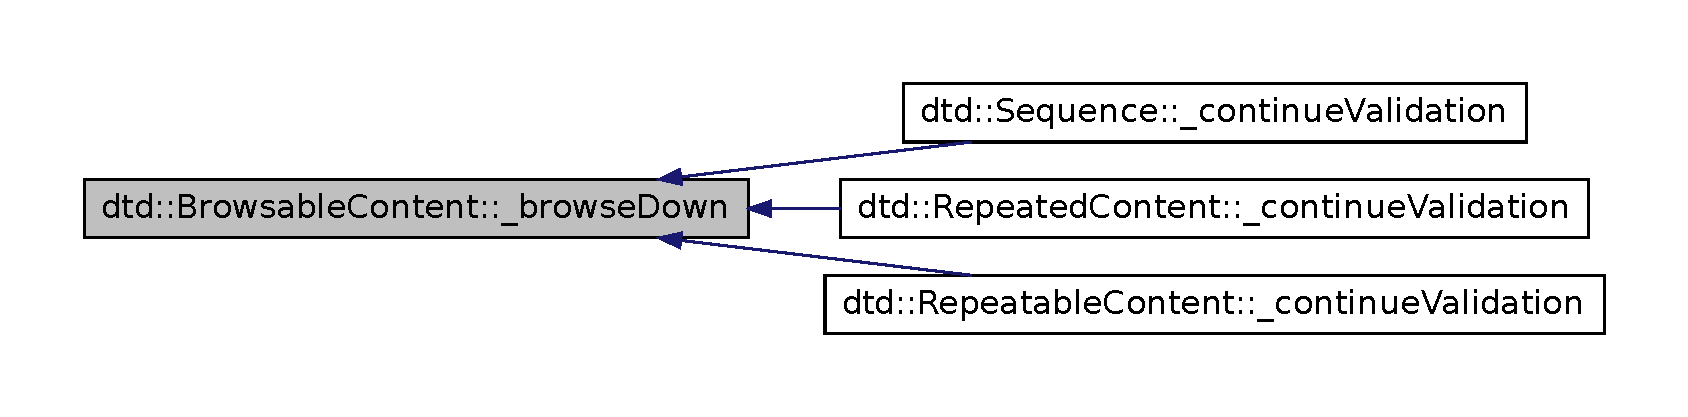
\includegraphics[width=400pt]{classdtd_1_1_browsable_content_aea818259a913cb7359d902ee121c4e87_icgraph}
\end{center}
\end{figure}


\hypertarget{classdtd_1_1_browsable_content_a267660fa668e638d6487a875ffd958b0}{
\index{dtd::BrowsableContent@{dtd::BrowsableContent}!\_\-browseUp@{\_\-browseUp}}
\index{\_\-browseUp@{\_\-browseUp}!dtd::BrowsableContent@{dtd::BrowsableContent}}
\subsubsection[{\_\-browseUp}]{\setlength{\rightskip}{0pt plus 5cm}bool dtd::BrowsableContent::\_\-browseUp (
\begin{DoxyParamCaption}
\item[{{\bf BrowsableContent} $\ast$}]{ parentContent, }
\item[{xml::CompositeMarkupNode::ChildrenIterator}]{ currentToken, }
\item[{xml::CompositeMarkupNode::ChildrenIterator}]{ endToken}
\end{DoxyParamCaption}
)\hspace{0.3cm}{\ttfamily  \mbox{[}protected\mbox{]}}}}
\label{classdtd_1_1_browsable_content_a267660fa668e638d6487a875ffd958b0}


Voici le graphe d'appel pour cette fonction :\nopagebreak
\begin{figure}[H]
\begin{center}
\leavevmode
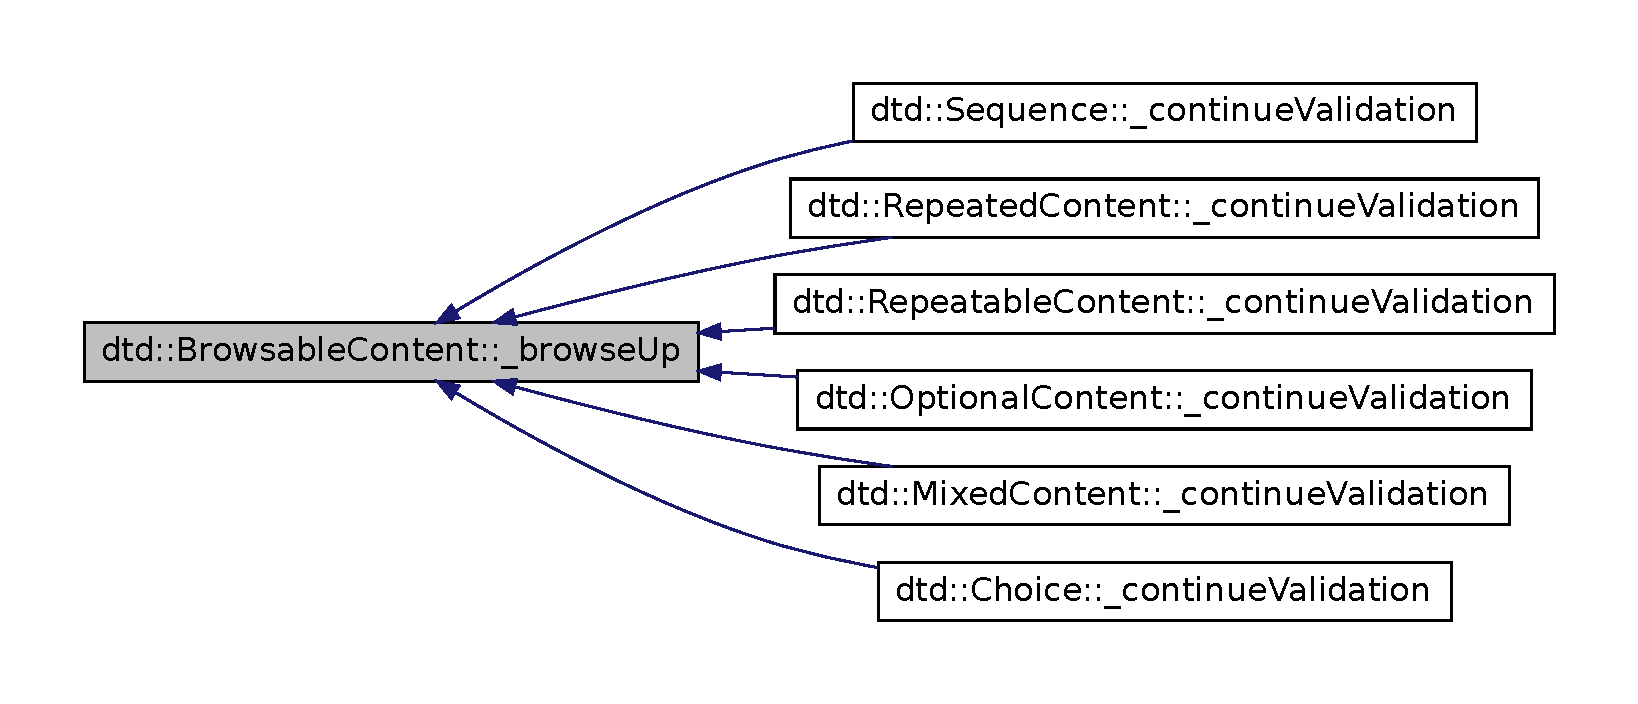
\includegraphics[width=400pt]{classdtd_1_1_browsable_content_a267660fa668e638d6487a875ffd958b0_icgraph}
\end{center}
\end{figure}


\hypertarget{classdtd_1_1_browsable_content_a6398e5990648e2af3fd775592b0d62ea}{
\index{dtd::BrowsableContent@{dtd::BrowsableContent}!\_\-continueValidation@{\_\-continueValidation}}
\index{\_\-continueValidation@{\_\-continueValidation}!dtd::BrowsableContent@{dtd::BrowsableContent}}
\subsubsection[{\_\-continueValidation}]{\setlength{\rightskip}{0pt plus 5cm}bool dtd::BrowsableContent::\_\-continueValidation (
\begin{DoxyParamCaption}
\item[{xml::CompositeMarkupNode::ChildrenIterator}]{ currentToken}
\end{DoxyParamCaption}
)\hspace{0.3cm}{\ttfamily  \mbox{[}protected, virtual\mbox{]}}}}
\label{classdtd_1_1_browsable_content_a6398e5990648e2af3fd775592b0d62ea}


Réimplémentée dans \hyperlink{classdtd_1_1_choice_a633d6ed16e627cfe31f602e7457bae72}{dtd::Choice}, \hyperlink{classdtd_1_1_mixed_content_a20d254e2b4366855818e1dd033d0736d}{dtd::MixedContent}, \hyperlink{classdtd_1_1_optional_content_ad299fdc7ddbac3df83c83cc93da8f6fe}{dtd::OptionalContent}, \hyperlink{classdtd_1_1_repeatable_content_af7cda09f207d691feec9846d757910c3}{dtd::RepeatableContent}, \hyperlink{classdtd_1_1_repeated_content_a3c3b6ab6dec9c12044e56198fc492db0}{dtd::RepeatedContent}, et \hyperlink{classdtd_1_1_sequence_a02874d51ebf3777a7fd16ee0e70b523b}{dtd::Sequence}.



Définition à la ligne 92 du fichier BrowsableContent.cpp.

\hypertarget{classdtd_1_1_browsable_content_a54a43ef27f874748f99b8ab71c23e2dc}{
\index{dtd::BrowsableContent@{dtd::BrowsableContent}!\_\-newValidation@{\_\-newValidation}}
\index{\_\-newValidation@{\_\-newValidation}!dtd::BrowsableContent@{dtd::BrowsableContent}}
\subsubsection[{\_\-newValidation}]{\setlength{\rightskip}{0pt plus 5cm}bool dtd::BrowsableContent::\_\-newValidation (
\begin{DoxyParamCaption}
\item[{xml::CompositeMarkupNode::ChildrenIterator}]{ firstToken, }
\item[{xml::CompositeMarkupNode::ChildrenIterator}]{ endToken, }
\item[{{\bf BrowsableContent} $\ast$}]{ nextStep}
\end{DoxyParamCaption}
)\hspace{0.3cm}{\ttfamily  \mbox{[}protected\mbox{]}}}}
\label{classdtd_1_1_browsable_content_a54a43ef27f874748f99b8ab71c23e2dc}
\hypertarget{classdtd_1_1_browsable_content_a67ab5a7329d94e363796ae2d17617246}{
\index{dtd::BrowsableContent@{dtd::BrowsableContent}!\_\-startValidation@{\_\-startValidation}}
\index{\_\-startValidation@{\_\-startValidation}!dtd::BrowsableContent@{dtd::BrowsableContent}}
\subsubsection[{\_\-startValidation}]{\setlength{\rightskip}{0pt plus 5cm}virtual bool dtd::BrowsableContent::\_\-startValidation (
\begin{DoxyParamCaption}
\item[{xml::CompositeMarkupNode::ChildrenIterator}]{ firstToken, }
\item[{xml::CompositeMarkupNode::ChildrenIterator}]{ endToken, }
\item[{{\bf BrowsableContent} $\ast$}]{ nextStep}
\end{DoxyParamCaption}
)\hspace{0.3cm}{\ttfamily  \mbox{[}protected, pure virtual\mbox{]}}}}
\label{classdtd_1_1_browsable_content_a67ab5a7329d94e363796ae2d17617246}


Implémenté dans \hyperlink{classdtd_1_1_choice_ab8d562a9912376d95a99a2ce3c9cd7f0}{dtd::Choice}, \hyperlink{classdtd_1_1_element_reference_a04d0141fbcfd0ff6171cd085c91e5622}{dtd::ElementReference}, \hyperlink{classdtd_1_1_mixed_content_ae2b12465df5873a58676315a563d1581}{dtd::MixedContent}, \hyperlink{classdtd_1_1_optional_content_aeb537bd54c1c717d11fd1bd60f8f1b8f}{dtd::OptionalContent}, \hyperlink{classdtd_1_1_repeatable_content_aa71e67d3e836b9ee0edc856c8dbc5f47}{dtd::RepeatableContent}, \hyperlink{classdtd_1_1_repeated_content_a3202c603a2cc800b6cbaf32880745dd3}{dtd::RepeatedContent}, \hyperlink{classdtd_1_1_sequence_a2765bc73d7fa4b92fafd60611e56e0f3}{dtd::Sequence}, et \hyperlink{classdtd_1_1_text_content_aa1f8d36777cd6b71686ee4db19268ae6}{dtd::TextContent}.

\hypertarget{classdtd_1_1_browsable_content_adbd9d013e126d5a1b601c3d781181bd4}{
\index{dtd::BrowsableContent@{dtd::BrowsableContent}!validate@{validate}}
\index{validate@{validate}!dtd::BrowsableContent@{dtd::BrowsableContent}}
\subsubsection[{validate}]{\setlength{\rightskip}{0pt plus 5cm}virtual bool dtd::BrowsableContent::validate (
\begin{DoxyParamCaption}
\item[{const xml::MarkupNode \&}]{ node}
\end{DoxyParamCaption}
)\hspace{0.3cm}{\ttfamily  \mbox{[}virtual\mbox{]}}}}
\label{classdtd_1_1_browsable_content_adbd9d013e126d5a1b601c3d781181bd4}


Implémente \hyperlink{classdtd_1_1_content_a2095fb10a09f6767aaf5e6da4b3018f1}{dtd::Content}.

\hypertarget{classdtd_1_1_browsable_content_a824a0c41b66aeea689e4283ee453d398}{
\index{dtd::BrowsableContent@{dtd::BrowsableContent}!validate@{validate}}
\index{validate@{validate}!dtd::BrowsableContent@{dtd::BrowsableContent}}
\subsubsection[{validate}]{\setlength{\rightskip}{0pt plus 5cm}virtual bool dtd::BrowsableContent::validate (
\begin{DoxyParamCaption}
\item[{const xml::CompositeMarkupNode \&}]{ node}
\end{DoxyParamCaption}
)\hspace{0.3cm}{\ttfamily  \mbox{[}virtual\mbox{]}}}}
\label{classdtd_1_1_browsable_content_a824a0c41b66aeea689e4283ee453d398}


Implémente \hyperlink{classdtd_1_1_content_acaa15daa3a3a2cf11632c4c93dc2cf37}{dtd::Content}.



Réimplémentée dans \hyperlink{classdtd_1_1_choice_ad0302d4e2b758025b430014fe8c20046}{dtd::Choice}, \hyperlink{classdtd_1_1_mixed_content_a675bca1039d5dd8cced7fddb856428fd}{dtd::MixedContent}, \hyperlink{classdtd_1_1_quantified_content_a83733f23442035bdbcd976723ed753a4}{dtd::QuantifiedContent}, et \hyperlink{classdtd_1_1_sequence_a585eecddf1104ba42a15944ee4ff4b19}{dtd::Sequence}.



La documentation de cette classe a été générée à partir des fichiers suivants :\begin{DoxyCompactItemize}
\item 
src/\hyperlink{_browsable_content_8hh}{BrowsableContent.hh}\item 
src/\hyperlink{_browsable_content_8cpp}{BrowsableContent.cpp}\end{DoxyCompactItemize}

\hypertarget{classdtd_1_1_choice}{
\section{Référence de la classe dtd::Choice}
\label{classdtd_1_1_choice}\index{dtd::Choice@{dtd::Choice}}
}


{\ttfamily \#include $<$Choice.hh$>$}



Graphe d'héritage de dtd::Choice:\nopagebreak
\begin{figure}[H]
\begin{center}
\leavevmode
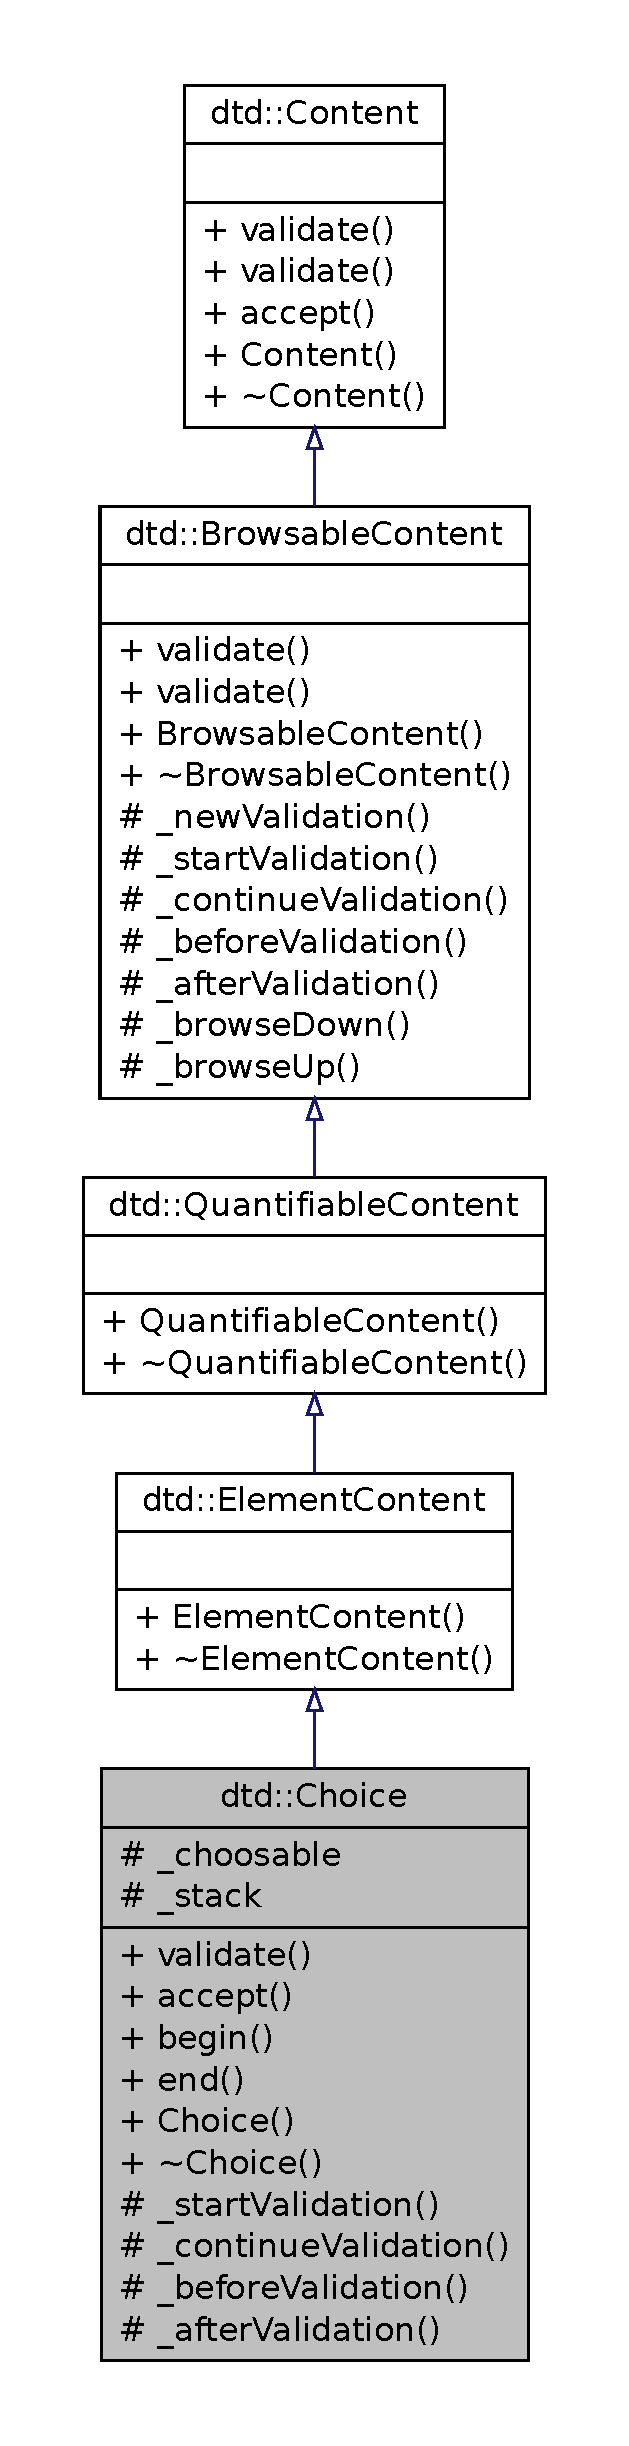
\includegraphics[height=600pt]{classdtd_1_1_choice__inherit__graph}
\end{center}
\end{figure}


Graphe de collaboration de dtd::Choice:\nopagebreak
\begin{figure}[H]
\begin{center}
\leavevmode
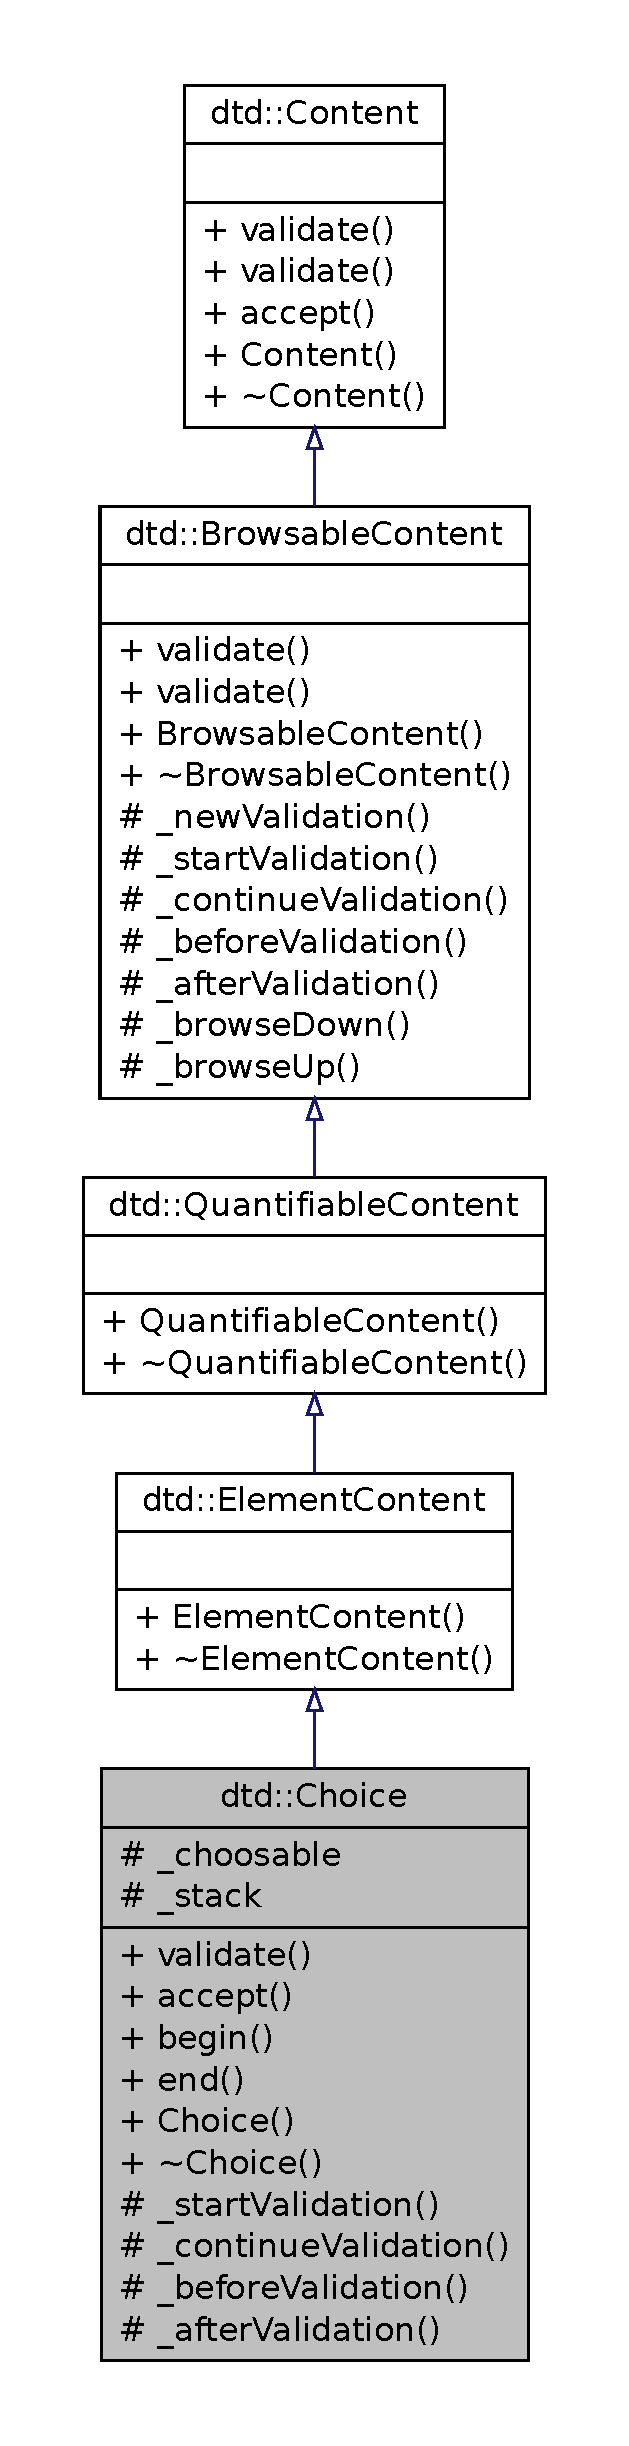
\includegraphics[height=600pt]{classdtd_1_1_choice__coll__graph}
\end{center}
\end{figure}
\subsection*{Classes}
\begin{DoxyCompactItemize}
\item 
struct \hyperlink{structdtd_1_1_choice_1_1___state}{\_\-State}
\end{DoxyCompactItemize}
\subsection*{Types publics}
\begin{DoxyCompactItemize}
\item 
typedef std::set$<$ \hyperlink{classdtd_1_1_element_content}{ElementContent} $\ast$ $>$ \hyperlink{classdtd_1_1_choice_af9629ca325eb99da3f274b2ad3dc2060}{ChoosableSet}
\item 
typedef \_\-ChoosableSet::const\_\-iterator \hyperlink{classdtd_1_1_choice_a127d277a680fe88ae37034deeefbfca4}{const\_\-iterator}
\end{DoxyCompactItemize}
\subsection*{Fonctions membres publiques}
\begin{DoxyCompactItemize}
\item 
virtual bool \hyperlink{classdtd_1_1_choice_ad0302d4e2b758025b430014fe8c20046}{validate} (const xml::CompositeMarkupNode \&node)
\item 
virtual void \hyperlink{classdtd_1_1_choice_a2eaed96716e6d7583c4b64f514c71b9d}{accept} (\hyperlink{classdtd_1_1_interface_d_t_d_visitor}{InterfaceDTDVisitor} \&visitor) const 
\item 
\hyperlink{classdtd_1_1_choice_a127d277a680fe88ae37034deeefbfca4}{const\_\-iterator} \hyperlink{classdtd_1_1_choice_afc189b482d6c53c47620ee23403205e0}{begin} () const 
\item 
\hyperlink{classdtd_1_1_choice_a127d277a680fe88ae37034deeefbfca4}{const\_\-iterator} \hyperlink{classdtd_1_1_choice_a65cea1b2b4c2ebb97650a0cc0153488e}{end} () const 
\item 
\hyperlink{classdtd_1_1_choice_a2d10476c9ccca603a8978d68de7957ca}{Choice} (const \hyperlink{classdtd_1_1_choice_af9629ca325eb99da3f274b2ad3dc2060}{ChoosableSet} \&elements)
\item 
virtual \hyperlink{classdtd_1_1_choice_ace8ec16e92018c56abda356776293f60}{$\sim$Choice} ()
\end{DoxyCompactItemize}
\subsection*{Types protégés}
\begin{DoxyCompactItemize}
\item 
typedef std::set$<$ \hyperlink{classdtd_1_1_element_content}{ElementContent} $\ast$ $>$ \hyperlink{classdtd_1_1_choice_a07352a0a4e78923e41370e6b00af1c86}{\_\-ChoosableSet}
\item 
typedef std::stack$<$ \hyperlink{structdtd_1_1_choice_1_1___state}{\_\-State} $>$ \hyperlink{classdtd_1_1_choice_a804cc83d915d4a96b04a850cf99b7b51}{\_\-StatesStack}
\end{DoxyCompactItemize}
\subsection*{Fonctions membres protégées}
\begin{DoxyCompactItemize}
\item 
virtual bool \hyperlink{classdtd_1_1_choice_ab8d562a9912376d95a99a2ce3c9cd7f0}{\_\-startValidation} (xml::CompositeMarkupNode::ChildrenIterator firstToken, xml::CompositeMarkupNode::ChildrenIterator endToken, \hyperlink{classdtd_1_1_browsable_content}{BrowsableContent} $\ast$nextStep)
\item 
virtual bool \hyperlink{classdtd_1_1_choice_a633d6ed16e627cfe31f602e7457bae72}{\_\-continueValidation} (xml::CompositeMarkupNode::ChildrenIterator currentToken)
\item 
virtual void \hyperlink{classdtd_1_1_choice_a4d7c2672e20a84741815e7065173b4e5}{\_\-beforeValidation} (xml::CompositeMarkupNode::ChildrenIterator firstToken, xml::CompositeMarkupNode::ChildrenIterator endToken, \hyperlink{classdtd_1_1_browsable_content}{BrowsableContent} $\ast$nextStep)
\item 
virtual void \hyperlink{classdtd_1_1_choice_a9183a9eb47b76a61ff77f89041751853}{\_\-afterValidation} ()
\end{DoxyCompactItemize}
\subsection*{Attributs protégés}
\begin{DoxyCompactItemize}
\item 
\hyperlink{classdtd_1_1_choice_a07352a0a4e78923e41370e6b00af1c86}{\_\-ChoosableSet} \hyperlink{classdtd_1_1_choice_aa6eb4aa595f08f84b243d349f4fbdb2d}{\_\-choosable}
\item 
\hyperlink{classdtd_1_1_choice_a804cc83d915d4a96b04a850cf99b7b51}{\_\-StatesStack} \hyperlink{classdtd_1_1_choice_a02a69def9aec60304827d57342158be6}{\_\-stack}
\end{DoxyCompactItemize}


\subsection{Description détaillée}


Définition à la ligne 20 du fichier Choice.hh.



\subsection{Documentation des définitions de type membres}
\hypertarget{classdtd_1_1_choice_a07352a0a4e78923e41370e6b00af1c86}{
\index{dtd::Choice@{dtd::Choice}!\_\-ChoosableSet@{\_\-ChoosableSet}}
\index{\_\-ChoosableSet@{\_\-ChoosableSet}!dtd::Choice@{dtd::Choice}}
\subsubsection[{\_\-ChoosableSet}]{\setlength{\rightskip}{0pt plus 5cm}typedef std::set$<${\bf ElementContent}$\ast$$>$ {\bf dtd::Choice::\_\-ChoosableSet}\hspace{0.3cm}{\ttfamily  \mbox{[}protected\mbox{]}}}}
\label{classdtd_1_1_choice_a07352a0a4e78923e41370e6b00af1c86}


Définition à la ligne 23 du fichier Choice.hh.

\hypertarget{classdtd_1_1_choice_a804cc83d915d4a96b04a850cf99b7b51}{
\index{dtd::Choice@{dtd::Choice}!\_\-StatesStack@{\_\-StatesStack}}
\index{\_\-StatesStack@{\_\-StatesStack}!dtd::Choice@{dtd::Choice}}
\subsubsection[{\_\-StatesStack}]{\setlength{\rightskip}{0pt plus 5cm}typedef std::stack$<${\bf \_\-State}$>$ {\bf dtd::Choice::\_\-StatesStack}\hspace{0.3cm}{\ttfamily  \mbox{[}protected\mbox{]}}}}
\label{classdtd_1_1_choice_a804cc83d915d4a96b04a850cf99b7b51}


Définition à la ligne 92 du fichier Choice.hh.

\hypertarget{classdtd_1_1_choice_af9629ca325eb99da3f274b2ad3dc2060}{
\index{dtd::Choice@{dtd::Choice}!ChoosableSet@{ChoosableSet}}
\index{ChoosableSet@{ChoosableSet}!dtd::Choice@{dtd::Choice}}
\subsubsection[{ChoosableSet}]{\setlength{\rightskip}{0pt plus 5cm}typedef std::set$<${\bf ElementContent}$\ast$$>$ {\bf dtd::Choice::ChoosableSet}}}
\label{classdtd_1_1_choice_af9629ca325eb99da3f274b2ad3dc2060}


Définition à la ligne 28 du fichier Choice.hh.

\hypertarget{classdtd_1_1_choice_a127d277a680fe88ae37034deeefbfca4}{
\index{dtd::Choice@{dtd::Choice}!const\_\-iterator@{const\_\-iterator}}
\index{const\_\-iterator@{const\_\-iterator}!dtd::Choice@{dtd::Choice}}
\subsubsection[{const\_\-iterator}]{\setlength{\rightskip}{0pt plus 5cm}typedef \_\-ChoosableSet::const\_\-iterator {\bf dtd::Choice::const\_\-iterator}}}
\label{classdtd_1_1_choice_a127d277a680fe88ae37034deeefbfca4}


Définition à la ligne 29 du fichier Choice.hh.



\subsection{Documentation des constructeurs et destructeur}
\hypertarget{classdtd_1_1_choice_a2d10476c9ccca603a8978d68de7957ca}{
\index{dtd::Choice@{dtd::Choice}!Choice@{Choice}}
\index{Choice@{Choice}!dtd::Choice@{dtd::Choice}}
\subsubsection[{Choice}]{\setlength{\rightskip}{0pt plus 5cm}dtd::Choice::Choice (
\begin{DoxyParamCaption}
\item[{const {\bf ChoosableSet} \&}]{ elements}
\end{DoxyParamCaption}
)}}
\label{classdtd_1_1_choice_a2d10476c9ccca603a8978d68de7957ca}


Définition à la ligne 59 du fichier Choice.cpp.

\hypertarget{classdtd_1_1_choice_ace8ec16e92018c56abda356776293f60}{
\index{dtd::Choice@{dtd::Choice}!$\sim$Choice@{$\sim$Choice}}
\index{$\sim$Choice@{$\sim$Choice}!dtd::Choice@{dtd::Choice}}
\subsubsection[{$\sim$Choice}]{\setlength{\rightskip}{0pt plus 5cm}dtd::Choice::$\sim$Choice (
\begin{DoxyParamCaption}
{}
\end{DoxyParamCaption}
)\hspace{0.3cm}{\ttfamily  \mbox{[}virtual\mbox{]}}}}
\label{classdtd_1_1_choice_ace8ec16e92018c56abda356776293f60}


Définition à la ligne 65 du fichier Choice.cpp.



\subsection{Documentation des fonctions membres}
\hypertarget{classdtd_1_1_choice_a9183a9eb47b76a61ff77f89041751853}{
\index{dtd::Choice@{dtd::Choice}!\_\-afterValidation@{\_\-afterValidation}}
\index{\_\-afterValidation@{\_\-afterValidation}!dtd::Choice@{dtd::Choice}}
\subsubsection[{\_\-afterValidation}]{\setlength{\rightskip}{0pt plus 5cm}void dtd::Choice::\_\-afterValidation (
\begin{DoxyParamCaption}
{}
\end{DoxyParamCaption}
)\hspace{0.3cm}{\ttfamily  \mbox{[}protected, virtual\mbox{]}}}}
\label{classdtd_1_1_choice_a9183a9eb47b76a61ff77f89041751853}


Réimplémentée à partir de \hyperlink{classdtd_1_1_browsable_content_a378fc620af75eb9bad9f37c663e3838d}{dtd::BrowsableContent}.



Définition à la ligne 85 du fichier Choice.cpp.

\hypertarget{classdtd_1_1_choice_a4d7c2672e20a84741815e7065173b4e5}{
\index{dtd::Choice@{dtd::Choice}!\_\-beforeValidation@{\_\-beforeValidation}}
\index{\_\-beforeValidation@{\_\-beforeValidation}!dtd::Choice@{dtd::Choice}}
\subsubsection[{\_\-beforeValidation}]{\setlength{\rightskip}{0pt plus 5cm}void dtd::Choice::\_\-beforeValidation (
\begin{DoxyParamCaption}
\item[{xml::CompositeMarkupNode::ChildrenIterator}]{ firstToken, }
\item[{xml::CompositeMarkupNode::ChildrenIterator}]{ endToken, }
\item[{{\bf BrowsableContent} $\ast$}]{ nextStep}
\end{DoxyParamCaption}
)\hspace{0.3cm}{\ttfamily  \mbox{[}protected, virtual\mbox{]}}}}
\label{classdtd_1_1_choice_a4d7c2672e20a84741815e7065173b4e5}


Réimplémentée à partir de \hyperlink{classdtd_1_1_browsable_content_ae9e55da18cc09557fc7896a7ccac2ee1}{dtd::BrowsableContent}.



Définition à la ligne 77 du fichier Choice.cpp.

\hypertarget{classdtd_1_1_choice_a633d6ed16e627cfe31f602e7457bae72}{
\index{dtd::Choice@{dtd::Choice}!\_\-continueValidation@{\_\-continueValidation}}
\index{\_\-continueValidation@{\_\-continueValidation}!dtd::Choice@{dtd::Choice}}
\subsubsection[{\_\-continueValidation}]{\setlength{\rightskip}{0pt plus 5cm}bool dtd::Choice::\_\-continueValidation (
\begin{DoxyParamCaption}
\item[{xml::CompositeMarkupNode::ChildrenIterator}]{ currentToken}
\end{DoxyParamCaption}
)\hspace{0.3cm}{\ttfamily  \mbox{[}protected, virtual\mbox{]}}}}
\label{classdtd_1_1_choice_a633d6ed16e627cfe31f602e7457bae72}


Réimplémentée à partir de \hyperlink{classdtd_1_1_browsable_content_a6398e5990648e2af3fd775592b0d62ea}{dtd::BrowsableContent}.



Définition à la ligne 109 du fichier Choice.cpp.



Voici le graphe d'appel pour cette fonction :\nopagebreak
\begin{figure}[H]
\begin{center}
\leavevmode
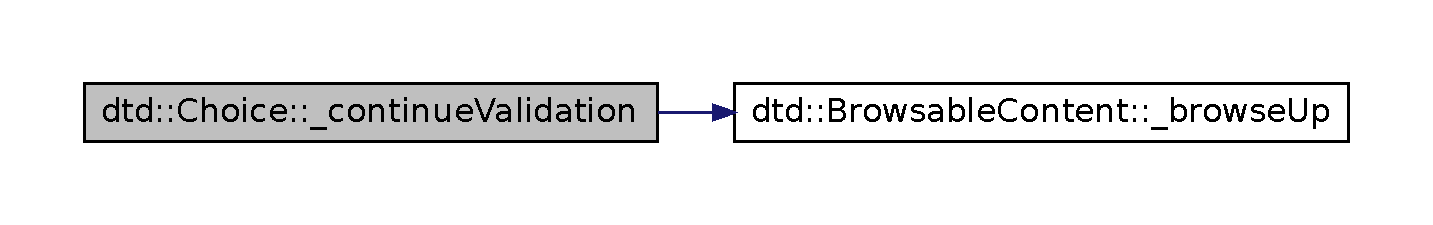
\includegraphics[width=400pt]{classdtd_1_1_choice_a633d6ed16e627cfe31f602e7457bae72_cgraph}
\end{center}
\end{figure}


\hypertarget{classdtd_1_1_choice_ab8d562a9912376d95a99a2ce3c9cd7f0}{
\index{dtd::Choice@{dtd::Choice}!\_\-startValidation@{\_\-startValidation}}
\index{\_\-startValidation@{\_\-startValidation}!dtd::Choice@{dtd::Choice}}
\subsubsection[{\_\-startValidation}]{\setlength{\rightskip}{0pt plus 5cm}virtual bool dtd::Choice::\_\-startValidation (
\begin{DoxyParamCaption}
\item[{xml::CompositeMarkupNode::ChildrenIterator}]{ firstToken, }
\item[{xml::CompositeMarkupNode::ChildrenIterator}]{ endToken, }
\item[{{\bf BrowsableContent} $\ast$}]{ nextStep}
\end{DoxyParamCaption}
)\hspace{0.3cm}{\ttfamily  \mbox{[}protected, virtual\mbox{]}}}}
\label{classdtd_1_1_choice_ab8d562a9912376d95a99a2ce3c9cd7f0}


Implémente \hyperlink{classdtd_1_1_browsable_content_a67ab5a7329d94e363796ae2d17617246}{dtd::BrowsableContent}.

\hypertarget{classdtd_1_1_choice_a2eaed96716e6d7583c4b64f514c71b9d}{
\index{dtd::Choice@{dtd::Choice}!accept@{accept}}
\index{accept@{accept}!dtd::Choice@{dtd::Choice}}
\subsubsection[{accept}]{\setlength{\rightskip}{0pt plus 5cm}void dtd::Choice::accept (
\begin{DoxyParamCaption}
\item[{{\bf InterfaceDTDVisitor} \&}]{ visitor}
\end{DoxyParamCaption}
) const\hspace{0.3cm}{\ttfamily  \mbox{[}virtual\mbox{]}}}}
\label{classdtd_1_1_choice_a2eaed96716e6d7583c4b64f514c71b9d}


Implémente \hyperlink{classdtd_1_1_content_a403cc15f12eaa187ad493fa600540cd8}{dtd::Content}.



Définition à la ligne 40 du fichier Choice.cpp.



Voici le graphe d'appel pour cette fonction :\nopagebreak
\begin{figure}[H]
\begin{center}
\leavevmode
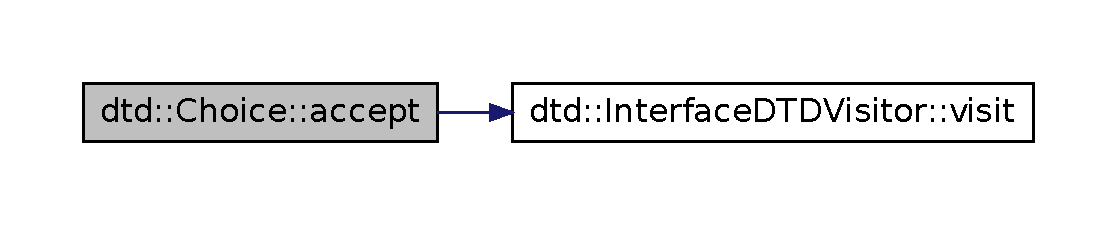
\includegraphics[width=400pt]{classdtd_1_1_choice_a2eaed96716e6d7583c4b64f514c71b9d_cgraph}
\end{center}
\end{figure}


\hypertarget{classdtd_1_1_choice_afc189b482d6c53c47620ee23403205e0}{
\index{dtd::Choice@{dtd::Choice}!begin@{begin}}
\index{begin@{begin}!dtd::Choice@{dtd::Choice}}
\subsubsection[{begin}]{\setlength{\rightskip}{0pt plus 5cm}{\bf Choice::const\_\-iterator} dtd::Choice::begin (
\begin{DoxyParamCaption}
{}
\end{DoxyParamCaption}
) const}}
\label{classdtd_1_1_choice_afc189b482d6c53c47620ee23403205e0}


Définition à la ligne 45 du fichier Choice.cpp.

\hypertarget{classdtd_1_1_choice_a65cea1b2b4c2ebb97650a0cc0153488e}{
\index{dtd::Choice@{dtd::Choice}!end@{end}}
\index{end@{end}!dtd::Choice@{dtd::Choice}}
\subsubsection[{end}]{\setlength{\rightskip}{0pt plus 5cm}{\bf Choice::const\_\-iterator} dtd::Choice::end (
\begin{DoxyParamCaption}
{}
\end{DoxyParamCaption}
) const}}
\label{classdtd_1_1_choice_a65cea1b2b4c2ebb97650a0cc0153488e}


Définition à la ligne 50 du fichier Choice.cpp.

\hypertarget{classdtd_1_1_choice_ad0302d4e2b758025b430014fe8c20046}{
\index{dtd::Choice@{dtd::Choice}!validate@{validate}}
\index{validate@{validate}!dtd::Choice@{dtd::Choice}}
\subsubsection[{validate}]{\setlength{\rightskip}{0pt plus 5cm}virtual bool dtd::Choice::validate (
\begin{DoxyParamCaption}
\item[{const xml::CompositeMarkupNode \&}]{ node}
\end{DoxyParamCaption}
)\hspace{0.3cm}{\ttfamily  \mbox{[}virtual\mbox{]}}}}
\label{classdtd_1_1_choice_ad0302d4e2b758025b430014fe8c20046}


Réimplémentée à partir de \hyperlink{classdtd_1_1_browsable_content_a824a0c41b66aeea689e4283ee453d398}{dtd::BrowsableContent}.



\subsection{Documentation des données membres}
\hypertarget{classdtd_1_1_choice_aa6eb4aa595f08f84b243d349f4fbdb2d}{
\index{dtd::Choice@{dtd::Choice}!\_\-choosable@{\_\-choosable}}
\index{\_\-choosable@{\_\-choosable}!dtd::Choice@{dtd::Choice}}
\subsubsection[{\_\-choosable}]{\setlength{\rightskip}{0pt plus 5cm}{\bf \_\-ChoosableSet} {\bf dtd::Choice::\_\-choosable}\hspace{0.3cm}{\ttfamily  \mbox{[}protected\mbox{]}}}}
\label{classdtd_1_1_choice_aa6eb4aa595f08f84b243d349f4fbdb2d}


Définition à la ligne 76 du fichier Choice.hh.

\hypertarget{classdtd_1_1_choice_a02a69def9aec60304827d57342158be6}{
\index{dtd::Choice@{dtd::Choice}!\_\-stack@{\_\-stack}}
\index{\_\-stack@{\_\-stack}!dtd::Choice@{dtd::Choice}}
\subsubsection[{\_\-stack}]{\setlength{\rightskip}{0pt plus 5cm}{\bf \_\-StatesStack} {\bf dtd::Choice::\_\-stack}\hspace{0.3cm}{\ttfamily  \mbox{[}protected\mbox{]}}}}
\label{classdtd_1_1_choice_a02a69def9aec60304827d57342158be6}


Définition à la ligne 93 du fichier Choice.hh.



La documentation de cette classe a été générée à partir des fichiers suivants :\begin{DoxyCompactItemize}
\item 
src/\hyperlink{_choice_8hh}{Choice.hh}\item 
src/\hyperlink{_choice_8cpp}{Choice.cpp}\end{DoxyCompactItemize}

\hypertarget{classdtd_1_1_content}{
\section{Référence de la classe dtd::Content}
\label{classdtd_1_1_content}\index{dtd::Content@{dtd::Content}}
}


{\ttfamily \#include $<$Content.hh$>$}



Graphe d'héritage de dtd::Content:\nopagebreak
\begin{figure}[H]
\begin{center}
\leavevmode
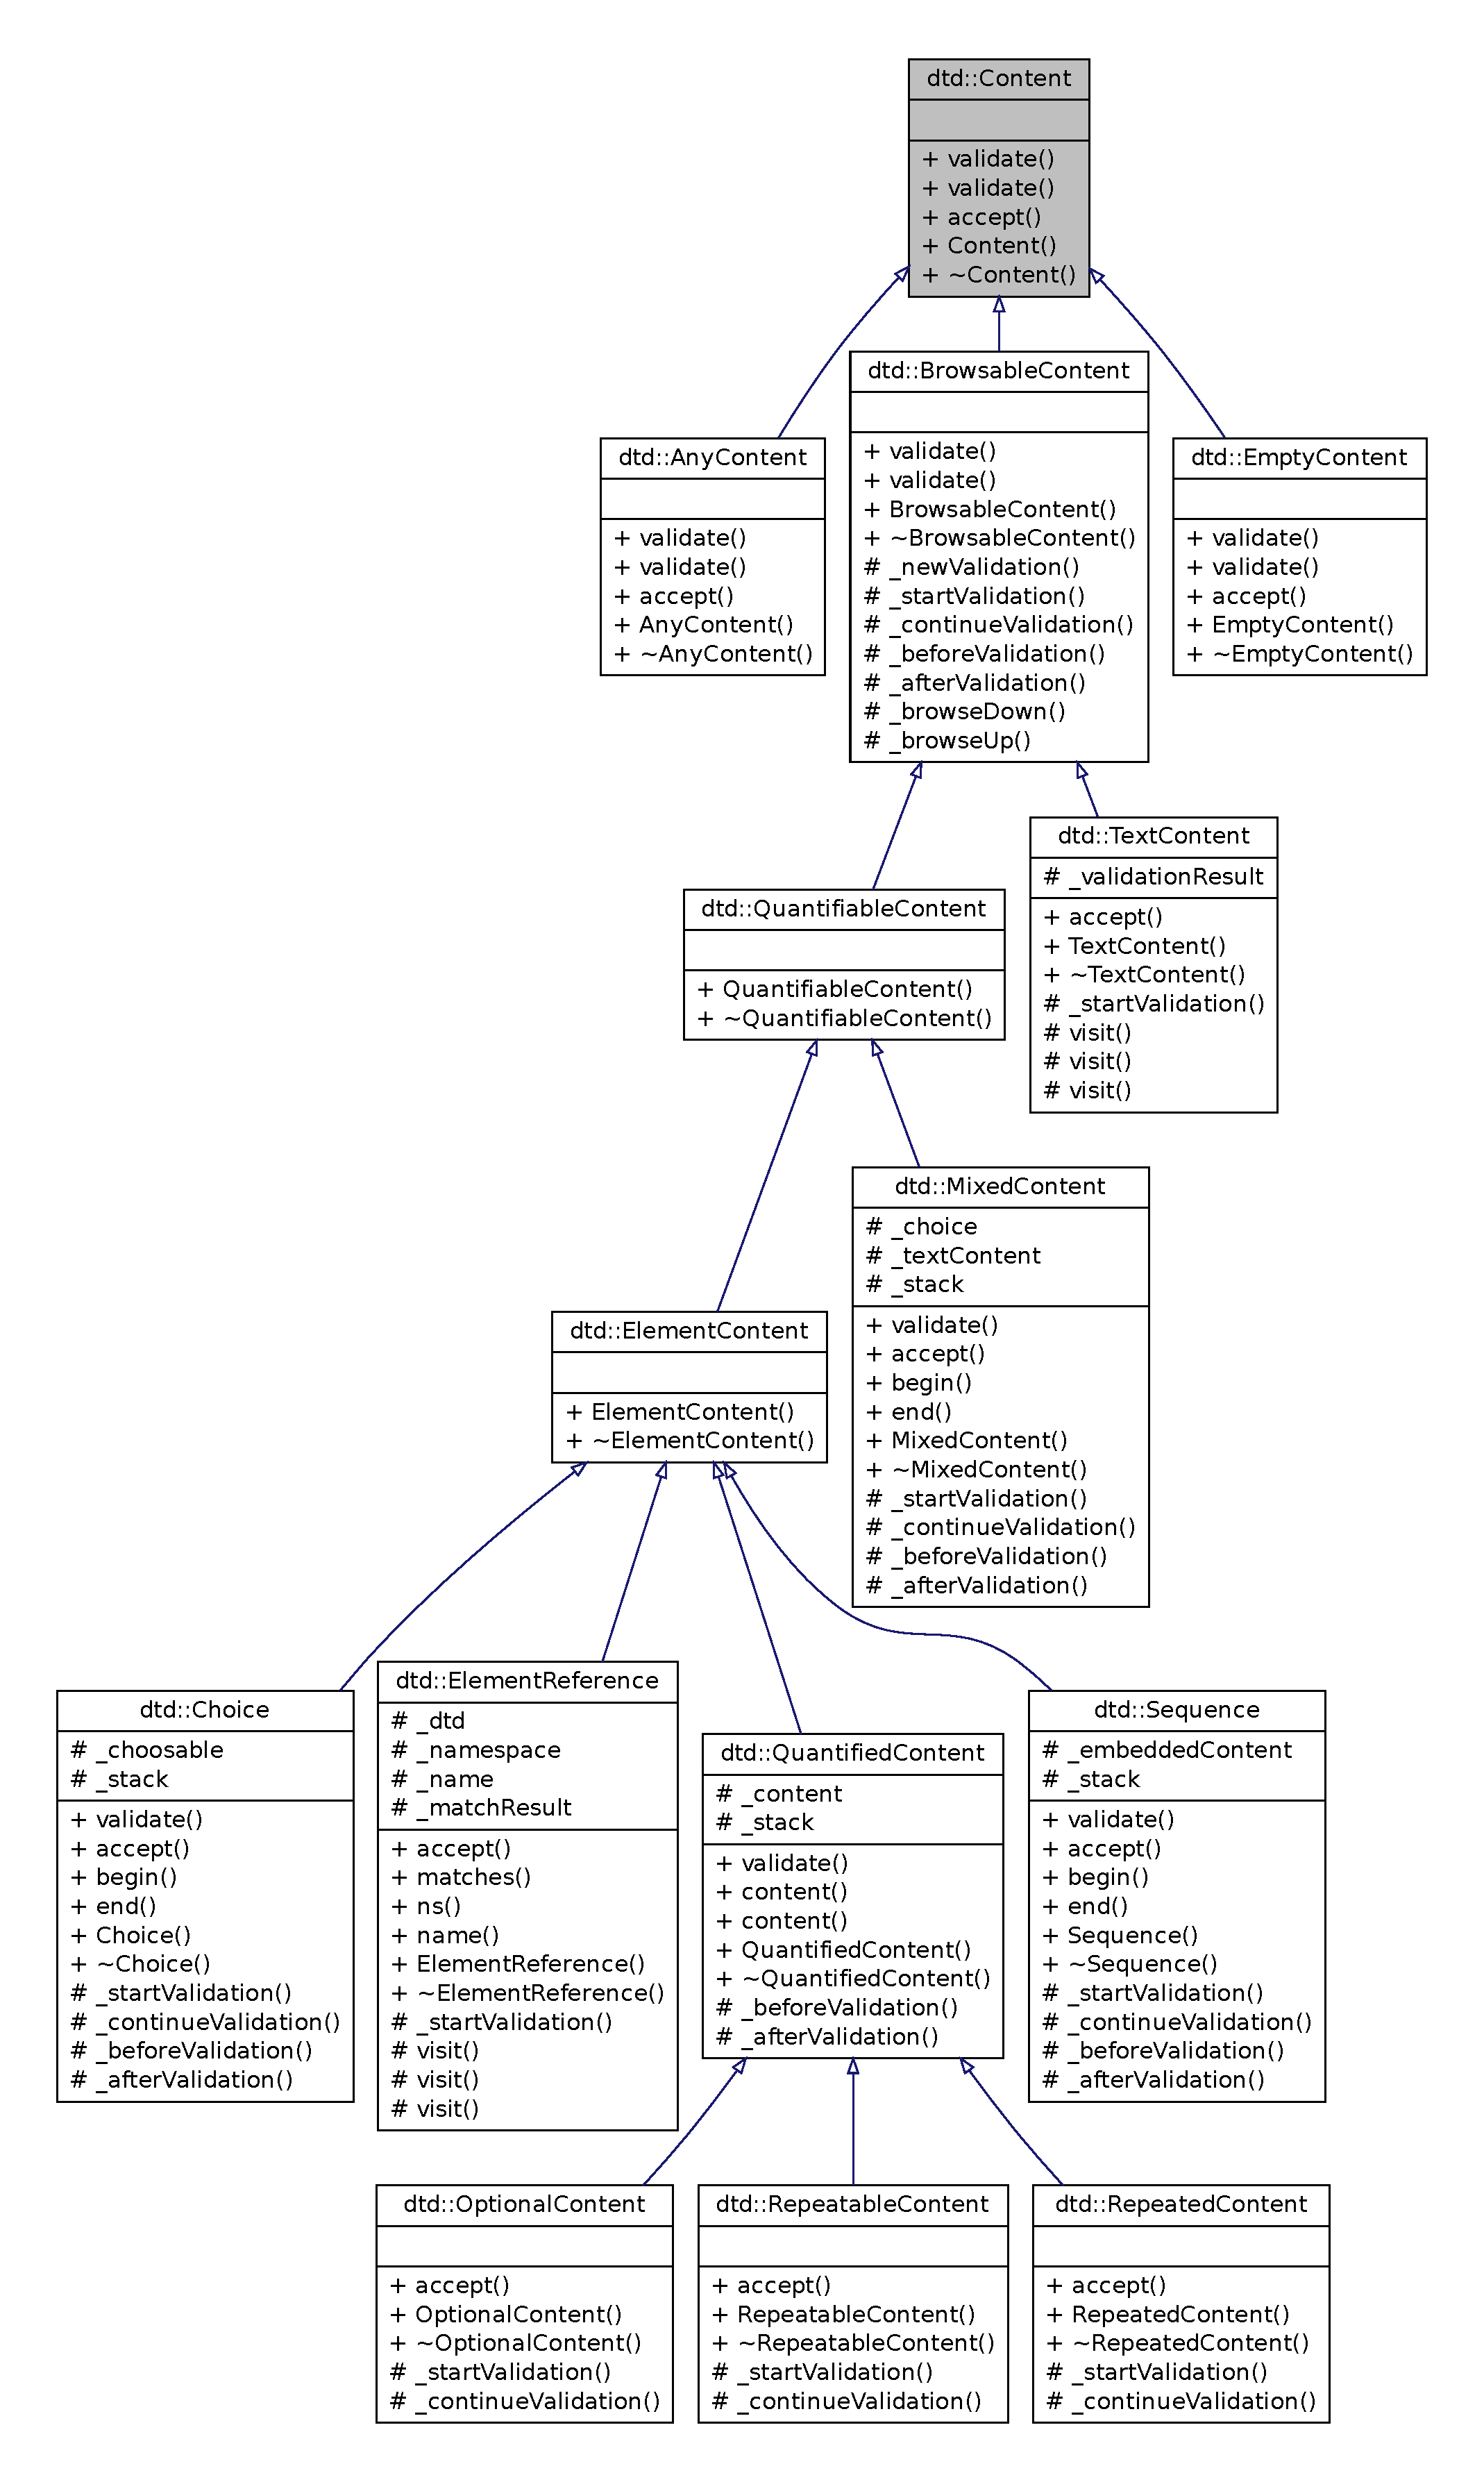
\includegraphics[height=600pt]{classdtd_1_1_content__inherit__graph}
\end{center}
\end{figure}
\subsection*{Fonctions membres publiques}
\begin{DoxyCompactItemize}
\item 
virtual bool \hyperlink{classdtd_1_1_content_a2095fb10a09f6767aaf5e6da4b3018f1}{validate} (const xml::MarkupNode \&node)=0
\item 
virtual bool \hyperlink{classdtd_1_1_content_acaa15daa3a3a2cf11632c4c93dc2cf37}{validate} (const xml::CompositeMarkupNode \&node)=0
\item 
virtual void \hyperlink{classdtd_1_1_content_a403cc15f12eaa187ad493fa600540cd8}{accept} (\hyperlink{classdtd_1_1_interface_d_t_d_visitor}{InterfaceDTDVisitor} \&visitor) const =0
\item 
\hyperlink{classdtd_1_1_content_ada40895a73972471e215054350e8ad2a}{Content} ()
\item 
virtual \hyperlink{classdtd_1_1_content_a75648214659cc2adb115cdaafefc0e37}{$\sim$Content} ()
\end{DoxyCompactItemize}


\subsection{Description détaillée}


Définition à la ligne 21 du fichier Content.hh.



\subsection{Documentation des constructeurs et destructeur}
\hypertarget{classdtd_1_1_content_ada40895a73972471e215054350e8ad2a}{
\index{dtd::Content@{dtd::Content}!Content@{Content}}
\index{Content@{Content}!dtd::Content@{dtd::Content}}
\subsubsection[{Content}]{\setlength{\rightskip}{0pt plus 5cm}dtd::Content::Content (
\begin{DoxyParamCaption}
{}
\end{DoxyParamCaption}
)}}
\label{classdtd_1_1_content_ada40895a73972471e215054350e8ad2a}


Définition à la ligne 38 du fichier Content.cpp.

\hypertarget{classdtd_1_1_content_a75648214659cc2adb115cdaafefc0e37}{
\index{dtd::Content@{dtd::Content}!$\sim$Content@{$\sim$Content}}
\index{$\sim$Content@{$\sim$Content}!dtd::Content@{dtd::Content}}
\subsubsection[{$\sim$Content}]{\setlength{\rightskip}{0pt plus 5cm}dtd::Content::$\sim$Content (
\begin{DoxyParamCaption}
{}
\end{DoxyParamCaption}
)\hspace{0.3cm}{\ttfamily  \mbox{[}virtual\mbox{]}}}}
\label{classdtd_1_1_content_a75648214659cc2adb115cdaafefc0e37}


Définition à la ligne 43 du fichier Content.cpp.



\subsection{Documentation des fonctions membres}
\hypertarget{classdtd_1_1_content_a403cc15f12eaa187ad493fa600540cd8}{
\index{dtd::Content@{dtd::Content}!accept@{accept}}
\index{accept@{accept}!dtd::Content@{dtd::Content}}
\subsubsection[{accept}]{\setlength{\rightskip}{0pt plus 5cm}virtual void dtd::Content::accept (
\begin{DoxyParamCaption}
\item[{{\bf InterfaceDTDVisitor} \&}]{ visitor}
\end{DoxyParamCaption}
) const\hspace{0.3cm}{\ttfamily  \mbox{[}pure virtual\mbox{]}}}}
\label{classdtd_1_1_content_a403cc15f12eaa187ad493fa600540cd8}


Implémenté dans \hyperlink{classdtd_1_1_any_content_ae9e5cecd79f91449de424a24944295cf}{dtd::AnyContent}, \hyperlink{classdtd_1_1_choice_a2eaed96716e6d7583c4b64f514c71b9d}{dtd::Choice}, \hyperlink{classdtd_1_1_element_reference_ade77978609f7a872d73c9507057f12a6}{dtd::ElementReference}, \hyperlink{classdtd_1_1_empty_content_a8440fe4e357b401e8db8d05baf59803e}{dtd::EmptyContent}, \hyperlink{classdtd_1_1_mixed_content_aea7a1312dc631047db037c84899f7a05}{dtd::MixedContent}, \hyperlink{classdtd_1_1_optional_content_a215be42249f1e54da514fdfc386ba21c}{dtd::OptionalContent}, \hyperlink{classdtd_1_1_repeatable_content_a28550745ec781816e4be44165dbb3934}{dtd::RepeatableContent}, \hyperlink{classdtd_1_1_repeated_content_af97dd8df71c00b1ec91d577671c8ed77}{dtd::RepeatedContent}, \hyperlink{classdtd_1_1_sequence_aa7ce2af63b36ed8be694d875488b108a}{dtd::Sequence}, et \hyperlink{classdtd_1_1_text_content_a5193fbafe92665d975b886a6ca18ac4f}{dtd::TextContent}.



Voici le graphe d'appel pour cette fonction :
\nopagebreak
\begin{figure}[H]
\begin{center}
\leavevmode
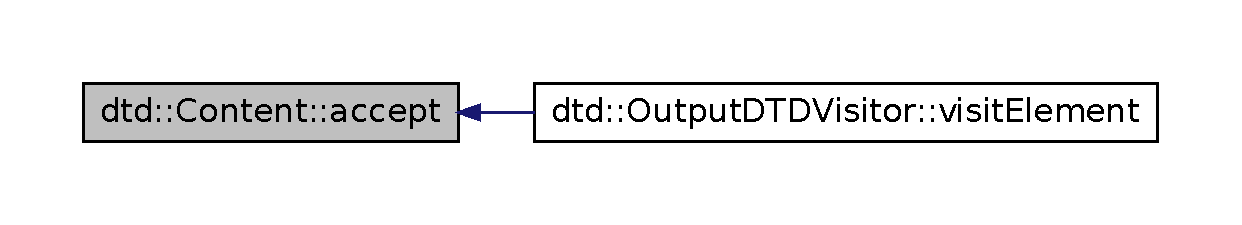
\includegraphics[width=400pt]{classdtd_1_1_content_a403cc15f12eaa187ad493fa600540cd8_icgraph}
\end{center}
\end{figure}


\hypertarget{classdtd_1_1_content_a2095fb10a09f6767aaf5e6da4b3018f1}{
\index{dtd::Content@{dtd::Content}!validate@{validate}}
\index{validate@{validate}!dtd::Content@{dtd::Content}}
\subsubsection[{validate}]{\setlength{\rightskip}{0pt plus 5cm}virtual bool dtd::Content::validate (
\begin{DoxyParamCaption}
\item[{const xml::MarkupNode \&}]{ node}
\end{DoxyParamCaption}
)\hspace{0.3cm}{\ttfamily  \mbox{[}pure virtual\mbox{]}}}}
\label{classdtd_1_1_content_a2095fb10a09f6767aaf5e6da4b3018f1}


Implémenté dans \hyperlink{classdtd_1_1_any_content_a1c69a5e152cec9428a72b83e1a86da67}{dtd::AnyContent}, \hyperlink{classdtd_1_1_browsable_content_adbd9d013e126d5a1b601c3d781181bd4}{dtd::BrowsableContent}, et \hyperlink{classdtd_1_1_empty_content_a763480d5964b94051f15a7ee5fbb936b}{dtd::EmptyContent}.

\hypertarget{classdtd_1_1_content_acaa15daa3a3a2cf11632c4c93dc2cf37}{
\index{dtd::Content@{dtd::Content}!validate@{validate}}
\index{validate@{validate}!dtd::Content@{dtd::Content}}
\subsubsection[{validate}]{\setlength{\rightskip}{0pt plus 5cm}virtual bool dtd::Content::validate (
\begin{DoxyParamCaption}
\item[{const xml::CompositeMarkupNode \&}]{ node}
\end{DoxyParamCaption}
)\hspace{0.3cm}{\ttfamily  \mbox{[}pure virtual\mbox{]}}}}
\label{classdtd_1_1_content_acaa15daa3a3a2cf11632c4c93dc2cf37}


Implémenté dans \hyperlink{classdtd_1_1_any_content_a6bd017d55e1c6eb09bdb7944afe57ab2}{dtd::AnyContent}, \hyperlink{classdtd_1_1_browsable_content_a824a0c41b66aeea689e4283ee453d398}{dtd::BrowsableContent}, \hyperlink{classdtd_1_1_choice_ad0302d4e2b758025b430014fe8c20046}{dtd::Choice}, \hyperlink{classdtd_1_1_empty_content_a97da0ccd8f6156b168f13759c920c6cc}{dtd::EmptyContent}, \hyperlink{classdtd_1_1_mixed_content_a675bca1039d5dd8cced7fddb856428fd}{dtd::MixedContent}, \hyperlink{classdtd_1_1_quantified_content_a83733f23442035bdbcd976723ed753a4}{dtd::QuantifiedContent}, et \hyperlink{classdtd_1_1_sequence_a585eecddf1104ba42a15944ee4ff4b19}{dtd::Sequence}.



La documentation de cette classe a été générée à partir des fichiers suivants :\begin{DoxyCompactItemize}
\item 
src/\hyperlink{_content_8hh}{Content.hh}\item 
src/\hyperlink{_content_8cpp}{Content.cpp}\end{DoxyCompactItemize}

\hypertarget{classdtd_1_1_d_t_d}{
\section{Référence de la classe dtd::DTD}
\label{classdtd_1_1_d_t_d}\index{dtd::DTD@{dtd::DTD}}
}


{\ttfamily \#include $<$DTD.hh$>$}

\subsection*{Fonctions membres publiques}
\begin{DoxyCompactItemize}
\item 
void \hyperlink{classdtd_1_1_d_t_d_acc2b63dcafbab0567708dddadca859d4}{accept} (\hyperlink{classdtd_1_1_interface_d_t_d_visitor}{InterfaceDTDVisitor} \&visitor)
\item 
void \hyperlink{classdtd_1_1_d_t_d_a1b0ba56addc8425b8e3c996e1bdb8fc1}{addElement} (const std::string \&ns, const std::string \&elementName, \hyperlink{classdtd_1_1_content}{Content} \&content)
\item 
void \hyperlink{classdtd_1_1_d_t_d_aa36c8c04bbc0e770242e338774583c83}{addAttributesList} (const std::string \&ns, const std::string \&elementName, const \hyperlink{namespacedtd_a8d5d29abb5de0468925f321597f57f4b}{AttributesList} \&attribute)
\item 
bool \hyperlink{classdtd_1_1_d_t_d_ae05093e02a85c295d2fe1b04914ca9af}{isValid} (const xml::Node \&root, const std::string \&validRootName)
\item 
\hyperlink{classdtd_1_1_d_t_d_ab1ba4d2d6d7e9d3521c21c3581f0e090}{DTD} ()
\item 
virtual \hyperlink{classdtd_1_1_d_t_d_ad9b422dbdadb18a93d3b0c2c0c5c1399}{$\sim$DTD} ()
\end{DoxyCompactItemize}
\subsection*{Types protégés}
\begin{DoxyCompactItemize}
\item 
typedef std::pair$<$ std::string, std::string $>$ \hyperlink{classdtd_1_1_d_t_d_aebfee050799e642c65f08ff77cadfb4e}{\_\-ElementId}
\item 
typedef std::map$<$ \hyperlink{classdtd_1_1_d_t_d_aebfee050799e642c65f08ff77cadfb4e}{\_\-ElementId}, \hyperlink{classdtd_1_1_content}{Content} $\ast$ $>$ \hyperlink{classdtd_1_1_d_t_d_a3acb9bcea95d9ad98d14b7851b6151c1}{\_\-Elements}
\item 
typedef std::map$<$ \hyperlink{classdtd_1_1_d_t_d_aebfee050799e642c65f08ff77cadfb4e}{\_\-ElementId}, \hyperlink{namespacedtd_a8d5d29abb5de0468925f321597f57f4b}{AttributesList} $>$ \hyperlink{classdtd_1_1_d_t_d_ad0c96201d399a44b597764334d343752}{\_\-AttributesLists}
\end{DoxyCompactItemize}
\subsection*{Fonctions membres protégées}
\begin{DoxyCompactItemize}
\item 
virtual void \hyperlink{classdtd_1_1_d_t_d_afa42d6567898ce96adf1b31b1da235e8}{visit} (const xml::TextNode \&node)
\item 
virtual void \hyperlink{classdtd_1_1_d_t_d_a7b21ffe9e0af0c815abedde305f0c241}{visit} (const xml::MarkupNode \&node)
\item 
virtual void \hyperlink{classdtd_1_1_d_t_d_a46680bf029f0728fa10bb0568017f4ce}{visit} (const xml::CompositeMarkupNode \&node)
\item 
bool \hyperlink{classdtd_1_1_d_t_d_a65a0b095665ae232ef40f1b9aad50387}{checkAttributes} (const xml::MarkupNode \&node)
\item 
\hyperlink{classdtd_1_1_content}{Content} $\ast$ \hyperlink{classdtd_1_1_d_t_d_ab1d76ad625a6fd3b64a4306cdc14400c}{getElement} (std::string ns, std::string name) const 
\item 
const \hyperlink{namespacedtd_a8d5d29abb5de0468925f321597f57f4b}{AttributesList} $\ast$ \hyperlink{classdtd_1_1_d_t_d_a531a239b85845e41a0422c6a60e59f63}{getAttributesList} (std::string ns, std::string name) const 
\item 
bool \hyperlink{classdtd_1_1_d_t_d_a88b9e78103312ed1a7be0f644571606f}{\_\-isValid} (const xml::Node \&node)
\end{DoxyCompactItemize}
\subsection*{Attributs protégés}
\begin{DoxyCompactItemize}
\item 
\hyperlink{classdtd_1_1_d_t_d_a3acb9bcea95d9ad98d14b7851b6151c1}{\_\-Elements} \hyperlink{classdtd_1_1_d_t_d_ab28c987860b12e12e5b9e3c199b4a4fd}{\_\-elements}
\item 
\hyperlink{classdtd_1_1_d_t_d_ad0c96201d399a44b597764334d343752}{\_\-AttributesLists} \hyperlink{classdtd_1_1_d_t_d_aec11a99c5e351b44bbdef249500bb1ac}{\_\-attributesLists}
\item 
bool \hyperlink{classdtd_1_1_d_t_d_acd1f91b37ce5dd73597f880c08546d40}{\_\-validatingRoot}
\item 
std::string \hyperlink{classdtd_1_1_d_t_d_ae2c393aa68abc63e9c5afe34770a75f5}{\_\-validRootName}
\item 
bool \hyperlink{classdtd_1_1_d_t_d_a1d27a4c5f57f3eac45bba4207fb0fa2e}{\_\-lastNodeIsValid}
\end{DoxyCompactItemize}


\subsection{Description détaillée}


Définition à la ligne 24 du fichier DTD.hh.



\subsection{Documentation des définitions de type membres}
\hypertarget{classdtd_1_1_d_t_d_ad0c96201d399a44b597764334d343752}{
\index{dtd::DTD@{dtd::DTD}!\_\-AttributesLists@{\_\-AttributesLists}}
\index{\_\-AttributesLists@{\_\-AttributesLists}!dtd::DTD@{dtd::DTD}}
\subsubsection[{\_\-AttributesLists}]{\setlength{\rightskip}{0pt plus 5cm}typedef std::map$<${\bf \_\-ElementId}, {\bf AttributesList}$>$ {\bf dtd::DTD::\_\-AttributesLists}\hspace{0.3cm}{\ttfamily  \mbox{[}protected\mbox{]}}}}
\label{classdtd_1_1_d_t_d_ad0c96201d399a44b597764334d343752}


Définition à la ligne 81 du fichier DTD.hh.

\hypertarget{classdtd_1_1_d_t_d_aebfee050799e642c65f08ff77cadfb4e}{
\index{dtd::DTD@{dtd::DTD}!\_\-ElementId@{\_\-ElementId}}
\index{\_\-ElementId@{\_\-ElementId}!dtd::DTD@{dtd::DTD}}
\subsubsection[{\_\-ElementId}]{\setlength{\rightskip}{0pt plus 5cm}typedef std::pair$<$std::string, std::string$>$ {\bf dtd::DTD::\_\-ElementId}\hspace{0.3cm}{\ttfamily  \mbox{[}protected\mbox{]}}}}
\label{classdtd_1_1_d_t_d_aebfee050799e642c65f08ff77cadfb4e}


Définition à la ligne 79 du fichier DTD.hh.

\hypertarget{classdtd_1_1_d_t_d_a3acb9bcea95d9ad98d14b7851b6151c1}{
\index{dtd::DTD@{dtd::DTD}!\_\-Elements@{\_\-Elements}}
\index{\_\-Elements@{\_\-Elements}!dtd::DTD@{dtd::DTD}}
\subsubsection[{\_\-Elements}]{\setlength{\rightskip}{0pt plus 5cm}typedef std::map$<${\bf \_\-ElementId}, {\bf Content}$\ast$$>$ {\bf dtd::DTD::\_\-Elements}\hspace{0.3cm}{\ttfamily  \mbox{[}protected\mbox{]}}}}
\label{classdtd_1_1_d_t_d_a3acb9bcea95d9ad98d14b7851b6151c1}


Définition à la ligne 80 du fichier DTD.hh.



\subsection{Documentation des constructeurs et destructeur}
\hypertarget{classdtd_1_1_d_t_d_ab1ba4d2d6d7e9d3521c21c3581f0e090}{
\index{dtd::DTD@{dtd::DTD}!DTD@{DTD}}
\index{DTD@{DTD}!dtd::DTD@{dtd::DTD}}
\subsubsection[{DTD}]{\setlength{\rightskip}{0pt plus 5cm}dtd::DTD::DTD (
\begin{DoxyParamCaption}
{}
\end{DoxyParamCaption}
)}}
\label{classdtd_1_1_d_t_d_ab1ba4d2d6d7e9d3521c21c3581f0e090}


Définition à la ligne 134 du fichier DTD.cpp.

\hypertarget{classdtd_1_1_d_t_d_ad9b422dbdadb18a93d3b0c2c0c5c1399}{
\index{dtd::DTD@{dtd::DTD}!$\sim$DTD@{$\sim$DTD}}
\index{$\sim$DTD@{$\sim$DTD}!dtd::DTD@{dtd::DTD}}
\subsubsection[{$\sim$DTD}]{\setlength{\rightskip}{0pt plus 5cm}dtd::DTD::$\sim$DTD (
\begin{DoxyParamCaption}
{}
\end{DoxyParamCaption}
)\hspace{0.3cm}{\ttfamily  \mbox{[}virtual\mbox{]}}}}
\label{classdtd_1_1_d_t_d_ad9b422dbdadb18a93d3b0c2c0c5c1399}


Définition à la ligne 141 du fichier DTD.cpp.



\subsection{Documentation des fonctions membres}
\hypertarget{classdtd_1_1_d_t_d_a88b9e78103312ed1a7be0f644571606f}{
\index{dtd::DTD@{dtd::DTD}!\_\-isValid@{\_\-isValid}}
\index{\_\-isValid@{\_\-isValid}!dtd::DTD@{dtd::DTD}}
\subsubsection[{\_\-isValid}]{\setlength{\rightskip}{0pt plus 5cm}bool dtd::DTD::\_\-isValid (
\begin{DoxyParamCaption}
\item[{const xml::Node \&}]{ node}
\end{DoxyParamCaption}
)\hspace{0.3cm}{\ttfamily  \mbox{[}protected\mbox{]}}}}
\label{classdtd_1_1_d_t_d_a88b9e78103312ed1a7be0f644571606f}


Définition à la ligne 161 du fichier DTD.cpp.

\hypertarget{classdtd_1_1_d_t_d_acc2b63dcafbab0567708dddadca859d4}{
\index{dtd::DTD@{dtd::DTD}!accept@{accept}}
\index{accept@{accept}!dtd::DTD@{dtd::DTD}}
\subsubsection[{accept}]{\setlength{\rightskip}{0pt plus 5cm}void dtd::DTD::accept (
\begin{DoxyParamCaption}
\item[{{\bf InterfaceDTDVisitor} \&}]{ visitor}
\end{DoxyParamCaption}
)}}
\label{classdtd_1_1_d_t_d_acc2b63dcafbab0567708dddadca859d4}


Définition à la ligne 41 du fichier DTD.cpp.



Voici le graphe d'appel pour cette fonction :
\nopagebreak
\begin{figure}[H]
\begin{center}
\leavevmode
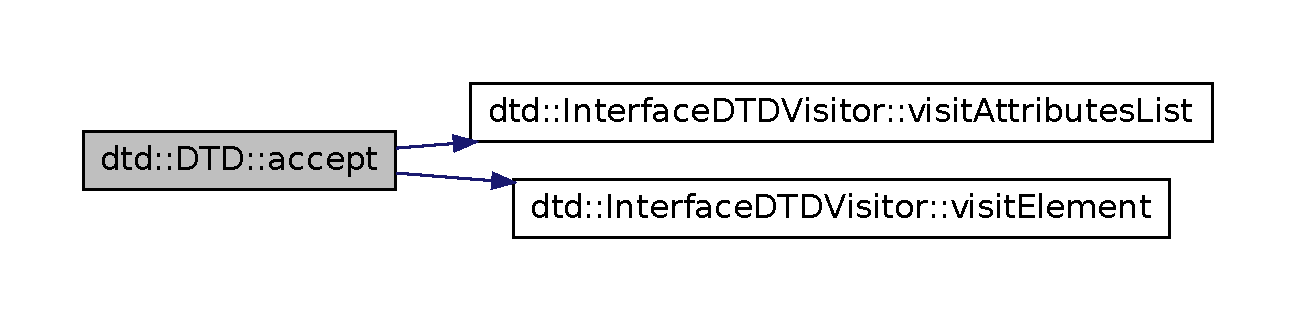
\includegraphics[width=400pt]{classdtd_1_1_d_t_d_acc2b63dcafbab0567708dddadca859d4_cgraph}
\end{center}
\end{figure}


\hypertarget{classdtd_1_1_d_t_d_aa36c8c04bbc0e770242e338774583c83}{
\index{dtd::DTD@{dtd::DTD}!addAttributesList@{addAttributesList}}
\index{addAttributesList@{addAttributesList}!dtd::DTD@{dtd::DTD}}
\subsubsection[{addAttributesList}]{\setlength{\rightskip}{0pt plus 5cm}void dtd::DTD::addAttributesList (
\begin{DoxyParamCaption}
\item[{const std::string \&}]{ ns, }
\item[{const std::string \&}]{ elementName, }
\item[{const {\bf AttributesList} \&}]{ attribute}
\end{DoxyParamCaption}
)}}
\label{classdtd_1_1_d_t_d_aa36c8c04bbc0e770242e338774583c83}


Définition à la ligne 71 du fichier DTD.cpp.

\hypertarget{classdtd_1_1_d_t_d_a1b0ba56addc8425b8e3c996e1bdb8fc1}{
\index{dtd::DTD@{dtd::DTD}!addElement@{addElement}}
\index{addElement@{addElement}!dtd::DTD@{dtd::DTD}}
\subsubsection[{addElement}]{\setlength{\rightskip}{0pt plus 5cm}void dtd::DTD::addElement (
\begin{DoxyParamCaption}
\item[{const std::string \&}]{ ns, }
\item[{const std::string \&}]{ elementName, }
\item[{{\bf Content} \&}]{ content}
\end{DoxyParamCaption}
)}}
\label{classdtd_1_1_d_t_d_a1b0ba56addc8425b8e3c996e1bdb8fc1}


Définition à la ligne 57 du fichier DTD.cpp.

\hypertarget{classdtd_1_1_d_t_d_a65a0b095665ae232ef40f1b9aad50387}{
\index{dtd::DTD@{dtd::DTD}!checkAttributes@{checkAttributes}}
\index{checkAttributes@{checkAttributes}!dtd::DTD@{dtd::DTD}}
\subsubsection[{checkAttributes}]{\setlength{\rightskip}{0pt plus 5cm}bool dtd::DTD::checkAttributes (
\begin{DoxyParamCaption}
\item[{const xml::MarkupNode \&}]{ node}
\end{DoxyParamCaption}
)\hspace{0.3cm}{\ttfamily  \mbox{[}protected\mbox{]}}}}
\label{classdtd_1_1_d_t_d_a65a0b095665ae232ef40f1b9aad50387}


Définition à la ligne 250 du fichier DTD.cpp.



Voici le graphe d'appel pour cette fonction :\nopagebreak
\begin{figure}[H]
\begin{center}
\leavevmode
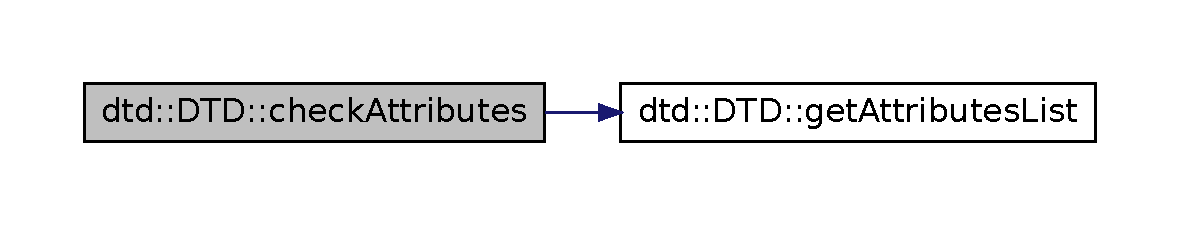
\includegraphics[width=400pt]{classdtd_1_1_d_t_d_a65a0b095665ae232ef40f1b9aad50387_cgraph}
\end{center}
\end{figure}


\hypertarget{classdtd_1_1_d_t_d_a531a239b85845e41a0422c6a60e59f63}{
\index{dtd::DTD@{dtd::DTD}!getAttributesList@{getAttributesList}}
\index{getAttributesList@{getAttributesList}!dtd::DTD@{dtd::DTD}}
\subsubsection[{getAttributesList}]{\setlength{\rightskip}{0pt plus 5cm}const {\bf AttributesList} $\ast$ dtd::DTD::getAttributesList (
\begin{DoxyParamCaption}
\item[{std::string}]{ ns, }
\item[{std::string}]{ name}
\end{DoxyParamCaption}
) const\hspace{0.3cm}{\ttfamily  \mbox{[}protected\mbox{]}}}}
\label{classdtd_1_1_d_t_d_a531a239b85845e41a0422c6a60e59f63}


Définition à la ligne 107 du fichier DTD.cpp.



Voici le graphe d'appel pour cette fonction :\nopagebreak
\begin{figure}[H]
\begin{center}
\leavevmode
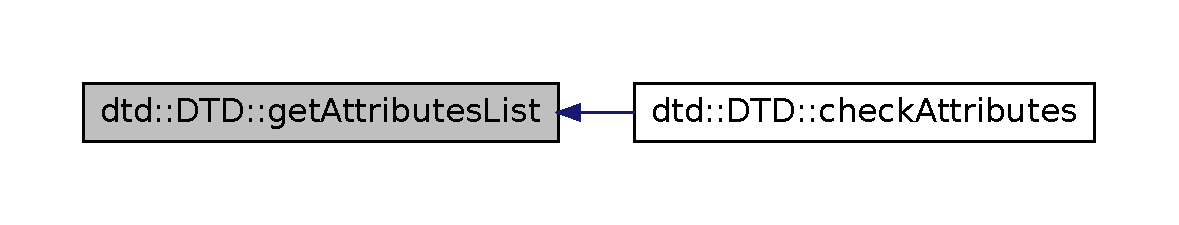
\includegraphics[width=400pt]{classdtd_1_1_d_t_d_a531a239b85845e41a0422c6a60e59f63_icgraph}
\end{center}
\end{figure}


\hypertarget{classdtd_1_1_d_t_d_ab1d76ad625a6fd3b64a4306cdc14400c}{
\index{dtd::DTD@{dtd::DTD}!getElement@{getElement}}
\index{getElement@{getElement}!dtd::DTD@{dtd::DTD}}
\subsubsection[{getElement}]{\setlength{\rightskip}{0pt plus 5cm}{\bf Content} $\ast$ dtd::DTD::getElement (
\begin{DoxyParamCaption}
\item[{std::string}]{ ns, }
\item[{std::string}]{ name}
\end{DoxyParamCaption}
) const\hspace{0.3cm}{\ttfamily  \mbox{[}protected\mbox{]}}}}
\label{classdtd_1_1_d_t_d_ab1d76ad625a6fd3b64a4306cdc14400c}


Définition à la ligne 92 du fichier DTD.cpp.

\hypertarget{classdtd_1_1_d_t_d_ae05093e02a85c295d2fe1b04914ca9af}{
\index{dtd::DTD@{dtd::DTD}!isValid@{isValid}}
\index{isValid@{isValid}!dtd::DTD@{dtd::DTD}}
\subsubsection[{isValid}]{\setlength{\rightskip}{0pt plus 5cm}bool dtd::DTD::isValid (
\begin{DoxyParamCaption}
\item[{const xml::Node \&}]{ root, }
\item[{const std::string \&}]{ validRootName}
\end{DoxyParamCaption}
)}}
\label{classdtd_1_1_d_t_d_ae05093e02a85c295d2fe1b04914ca9af}


Définition à la ligne 123 du fichier DTD.cpp.

\hypertarget{classdtd_1_1_d_t_d_a46680bf029f0728fa10bb0568017f4ce}{
\index{dtd::DTD@{dtd::DTD}!visit@{visit}}
\index{visit@{visit}!dtd::DTD@{dtd::DTD}}
\subsubsection[{visit}]{\setlength{\rightskip}{0pt plus 5cm}virtual void dtd::DTD::visit (
\begin{DoxyParamCaption}
\item[{const xml::CompositeMarkupNode \&}]{ node}
\end{DoxyParamCaption}
)\hspace{0.3cm}{\ttfamily  \mbox{[}protected, virtual\mbox{]}}}}
\label{classdtd_1_1_d_t_d_a46680bf029f0728fa10bb0568017f4ce}
\hypertarget{classdtd_1_1_d_t_d_afa42d6567898ce96adf1b31b1da235e8}{
\index{dtd::DTD@{dtd::DTD}!visit@{visit}}
\index{visit@{visit}!dtd::DTD@{dtd::DTD}}
\subsubsection[{visit}]{\setlength{\rightskip}{0pt plus 5cm}virtual void dtd::DTD::visit (
\begin{DoxyParamCaption}
\item[{const xml::TextNode \&}]{ node}
\end{DoxyParamCaption}
)\hspace{0.3cm}{\ttfamily  \mbox{[}protected, virtual\mbox{]}}}}
\label{classdtd_1_1_d_t_d_afa42d6567898ce96adf1b31b1da235e8}
\hypertarget{classdtd_1_1_d_t_d_a7b21ffe9e0af0c815abedde305f0c241}{
\index{dtd::DTD@{dtd::DTD}!visit@{visit}}
\index{visit@{visit}!dtd::DTD@{dtd::DTD}}
\subsubsection[{visit}]{\setlength{\rightskip}{0pt plus 5cm}virtual void dtd::DTD::visit (
\begin{DoxyParamCaption}
\item[{const xml::MarkupNode \&}]{ node}
\end{DoxyParamCaption}
)\hspace{0.3cm}{\ttfamily  \mbox{[}protected, virtual\mbox{]}}}}
\label{classdtd_1_1_d_t_d_a7b21ffe9e0af0c815abedde305f0c241}


\subsection{Documentation des données membres}
\hypertarget{classdtd_1_1_d_t_d_aec11a99c5e351b44bbdef249500bb1ac}{
\index{dtd::DTD@{dtd::DTD}!\_\-attributesLists@{\_\-attributesLists}}
\index{\_\-attributesLists@{\_\-attributesLists}!dtd::DTD@{dtd::DTD}}
\subsubsection[{\_\-attributesLists}]{\setlength{\rightskip}{0pt plus 5cm}{\bf \_\-AttributesLists} {\bf dtd::DTD::\_\-attributesLists}\hspace{0.3cm}{\ttfamily  \mbox{[}protected\mbox{]}}}}
\label{classdtd_1_1_d_t_d_aec11a99c5e351b44bbdef249500bb1ac}


Définition à la ligne 84 du fichier DTD.hh.

\hypertarget{classdtd_1_1_d_t_d_ab28c987860b12e12e5b9e3c199b4a4fd}{
\index{dtd::DTD@{dtd::DTD}!\_\-elements@{\_\-elements}}
\index{\_\-elements@{\_\-elements}!dtd::DTD@{dtd::DTD}}
\subsubsection[{\_\-elements}]{\setlength{\rightskip}{0pt plus 5cm}{\bf \_\-Elements} {\bf dtd::DTD::\_\-elements}\hspace{0.3cm}{\ttfamily  \mbox{[}protected\mbox{]}}}}
\label{classdtd_1_1_d_t_d_ab28c987860b12e12e5b9e3c199b4a4fd}


Définition à la ligne 83 du fichier DTD.hh.

\hypertarget{classdtd_1_1_d_t_d_a1d27a4c5f57f3eac45bba4207fb0fa2e}{
\index{dtd::DTD@{dtd::DTD}!\_\-lastNodeIsValid@{\_\-lastNodeIsValid}}
\index{\_\-lastNodeIsValid@{\_\-lastNodeIsValid}!dtd::DTD@{dtd::DTD}}
\subsubsection[{\_\-lastNodeIsValid}]{\setlength{\rightskip}{0pt plus 5cm}bool {\bf dtd::DTD::\_\-lastNodeIsValid}\hspace{0.3cm}{\ttfamily  \mbox{[}protected\mbox{]}}}}
\label{classdtd_1_1_d_t_d_a1d27a4c5f57f3eac45bba4207fb0fa2e}


Définition à la ligne 88 du fichier DTD.hh.

\hypertarget{classdtd_1_1_d_t_d_acd1f91b37ce5dd73597f880c08546d40}{
\index{dtd::DTD@{dtd::DTD}!\_\-validatingRoot@{\_\-validatingRoot}}
\index{\_\-validatingRoot@{\_\-validatingRoot}!dtd::DTD@{dtd::DTD}}
\subsubsection[{\_\-validatingRoot}]{\setlength{\rightskip}{0pt plus 5cm}bool {\bf dtd::DTD::\_\-validatingRoot}\hspace{0.3cm}{\ttfamily  \mbox{[}protected\mbox{]}}}}
\label{classdtd_1_1_d_t_d_acd1f91b37ce5dd73597f880c08546d40}


Définition à la ligne 86 du fichier DTD.hh.

\hypertarget{classdtd_1_1_d_t_d_ae2c393aa68abc63e9c5afe34770a75f5}{
\index{dtd::DTD@{dtd::DTD}!\_\-validRootName@{\_\-validRootName}}
\index{\_\-validRootName@{\_\-validRootName}!dtd::DTD@{dtd::DTD}}
\subsubsection[{\_\-validRootName}]{\setlength{\rightskip}{0pt plus 5cm}std::string {\bf dtd::DTD::\_\-validRootName}\hspace{0.3cm}{\ttfamily  \mbox{[}protected\mbox{]}}}}
\label{classdtd_1_1_d_t_d_ae2c393aa68abc63e9c5afe34770a75f5}


Définition à la ligne 87 du fichier DTD.hh.



La documentation de cette classe a été générée à partir des fichiers suivants :\begin{DoxyCompactItemize}
\item 
src/\hyperlink{_d_t_d_8hh}{DTD.hh}\item 
src/\hyperlink{_d_t_d_8cpp}{DTD.cpp}\end{DoxyCompactItemize}

\hypertarget{classdtd_1_1_element_content}{
\section{Référence de la classe dtd::ElementContent}
\label{classdtd_1_1_element_content}\index{dtd::ElementContent@{dtd::ElementContent}}
}


{\ttfamily \#include $<$ElementContent.hh$>$}



Graphe d'héritage de dtd::ElementContent:\nopagebreak
\begin{figure}[H]
\begin{center}
\leavevmode
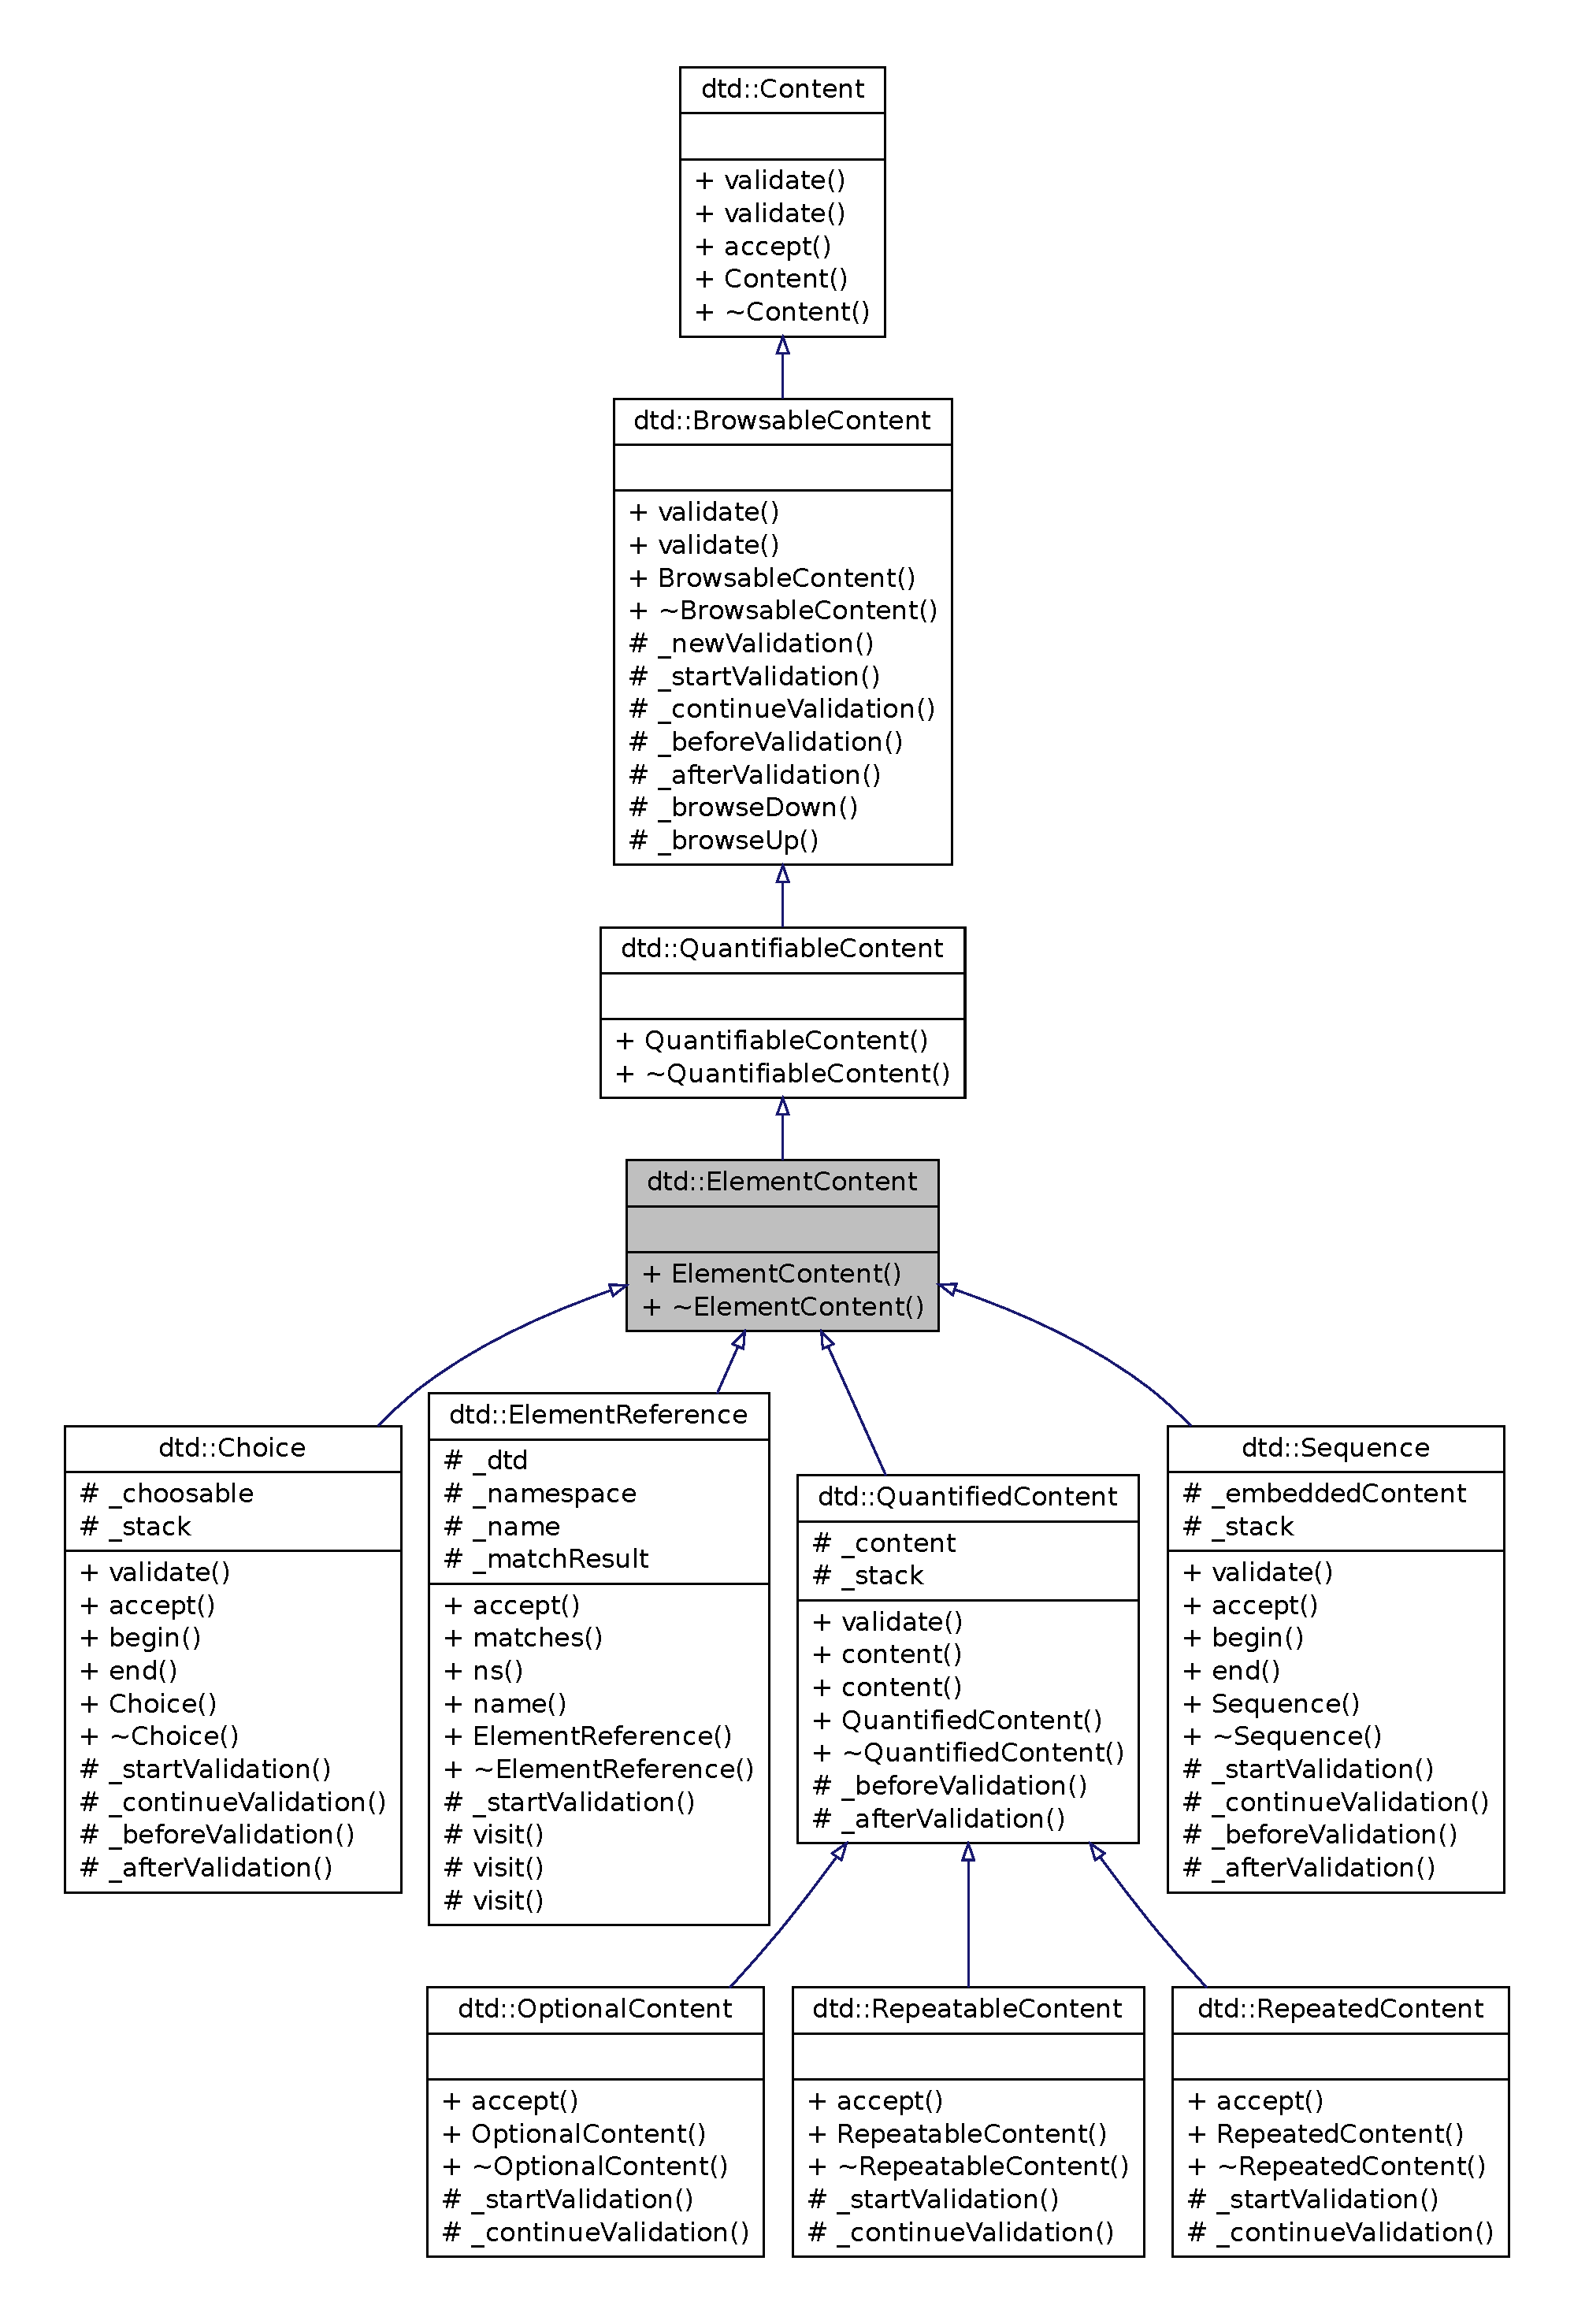
\includegraphics[width=400pt]{classdtd_1_1_element_content__inherit__graph}
\end{center}
\end{figure}


Graphe de collaboration de dtd::ElementContent:\nopagebreak
\begin{figure}[H]
\begin{center}
\leavevmode
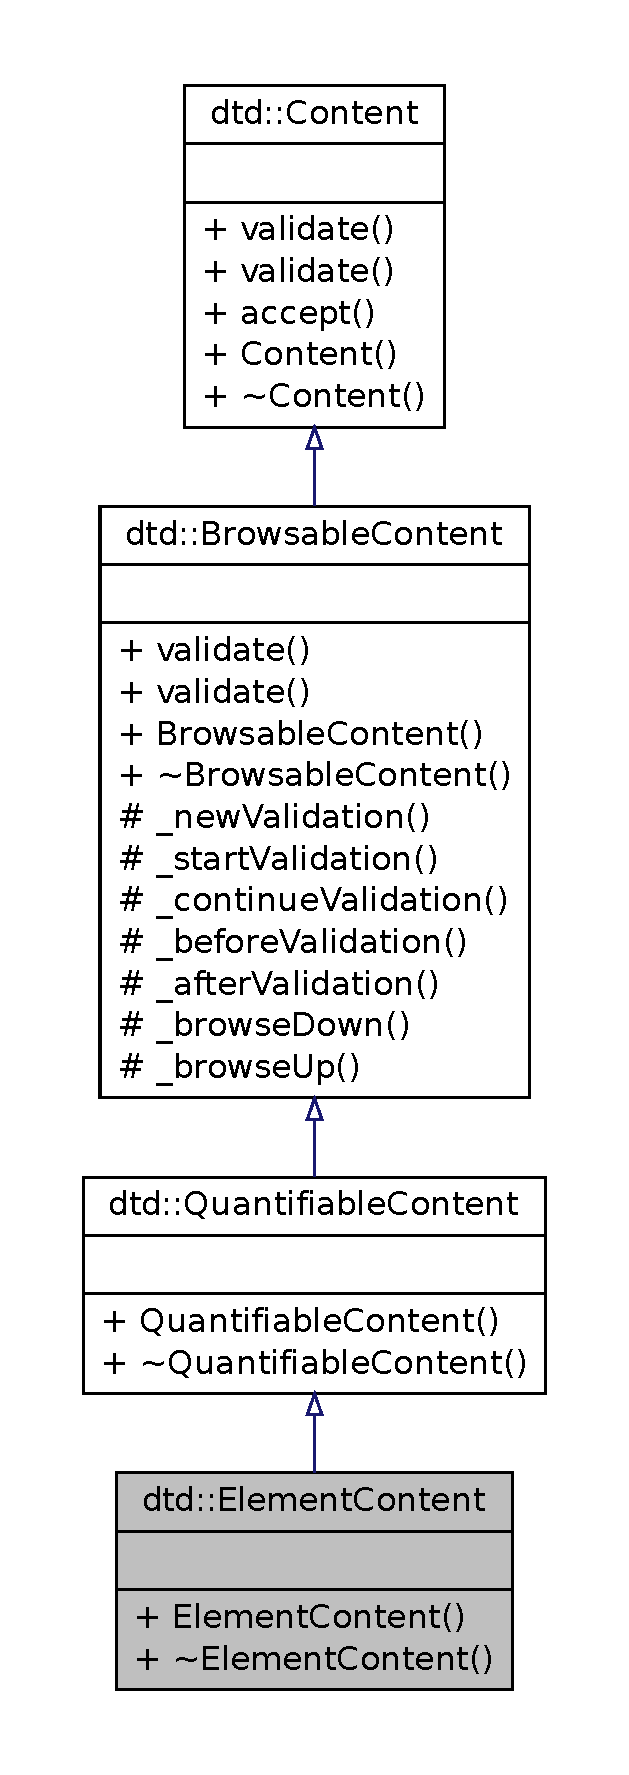
\includegraphics[height=600pt]{classdtd_1_1_element_content__coll__graph}
\end{center}
\end{figure}
\subsection*{Fonctions membres publiques}
\begin{DoxyCompactItemize}
\item 
\hyperlink{classdtd_1_1_element_content_a9965fae4a32ae334b22c5461d5d98505}{ElementContent} ()
\item 
virtual \hyperlink{classdtd_1_1_element_content_acd998d627ac4e99025d4c9f426719558}{$\sim$ElementContent} ()
\end{DoxyCompactItemize}


\subsection{Description détaillée}


Définition à la ligne 18 du fichier ElementContent.hh.



\subsection{Documentation des constructeurs et destructeur}
\hypertarget{classdtd_1_1_element_content_a9965fae4a32ae334b22c5461d5d98505}{
\index{dtd::ElementContent@{dtd::ElementContent}!ElementContent@{ElementContent}}
\index{ElementContent@{ElementContent}!dtd::ElementContent@{dtd::ElementContent}}
\subsubsection[{ElementContent}]{\setlength{\rightskip}{0pt plus 5cm}dtd::ElementContent::ElementContent (
\begin{DoxyParamCaption}
{}
\end{DoxyParamCaption}
)}}
\label{classdtd_1_1_element_content_a9965fae4a32ae334b22c5461d5d98505}


Définition à la ligne 36 du fichier ElementContent.cpp.

\hypertarget{classdtd_1_1_element_content_acd998d627ac4e99025d4c9f426719558}{
\index{dtd::ElementContent@{dtd::ElementContent}!$\sim$ElementContent@{$\sim$ElementContent}}
\index{$\sim$ElementContent@{$\sim$ElementContent}!dtd::ElementContent@{dtd::ElementContent}}
\subsubsection[{$\sim$ElementContent}]{\setlength{\rightskip}{0pt plus 5cm}dtd::ElementContent::$\sim$ElementContent (
\begin{DoxyParamCaption}
{}
\end{DoxyParamCaption}
)\hspace{0.3cm}{\ttfamily  \mbox{[}virtual\mbox{]}}}}
\label{classdtd_1_1_element_content_acd998d627ac4e99025d4c9f426719558}


Définition à la ligne 42 du fichier ElementContent.cpp.



La documentation de cette classe a été générée à partir des fichiers suivants :\begin{DoxyCompactItemize}
\item 
src/\hyperlink{_element_content_8hh}{ElementContent.hh}\item 
src/\hyperlink{_element_content_8cpp}{ElementContent.cpp}\end{DoxyCompactItemize}

\hypertarget{classdtd_1_1_element_reference}{
\section{Référence de la classe dtd::ElementReference}
\label{classdtd_1_1_element_reference}\index{dtd::ElementReference@{dtd::ElementReference}}
}


{\ttfamily \#include $<$ElementReference.hh$>$}



Graphe d'héritage de dtd::ElementReference:\nopagebreak
\begin{figure}[H]
\begin{center}
\leavevmode
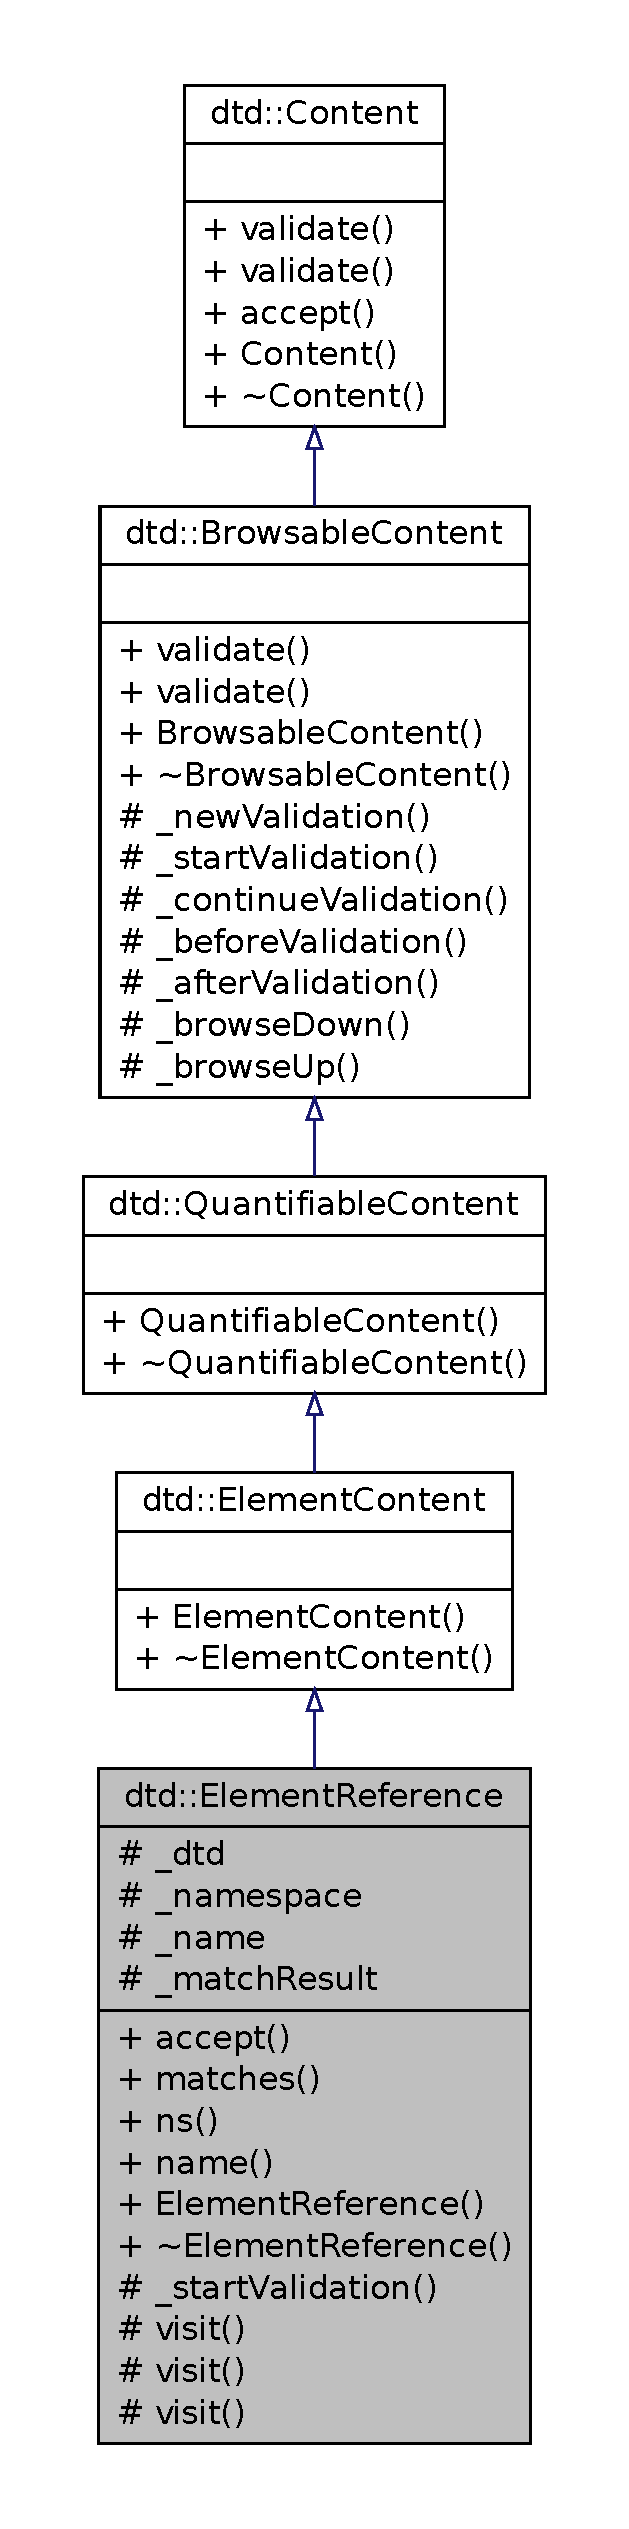
\includegraphics[height=600pt]{classdtd_1_1_element_reference__inherit__graph}
\end{center}
\end{figure}


Graphe de collaboration de dtd::ElementReference:
\nopagebreak
\begin{figure}[H]
\begin{center}
\leavevmode
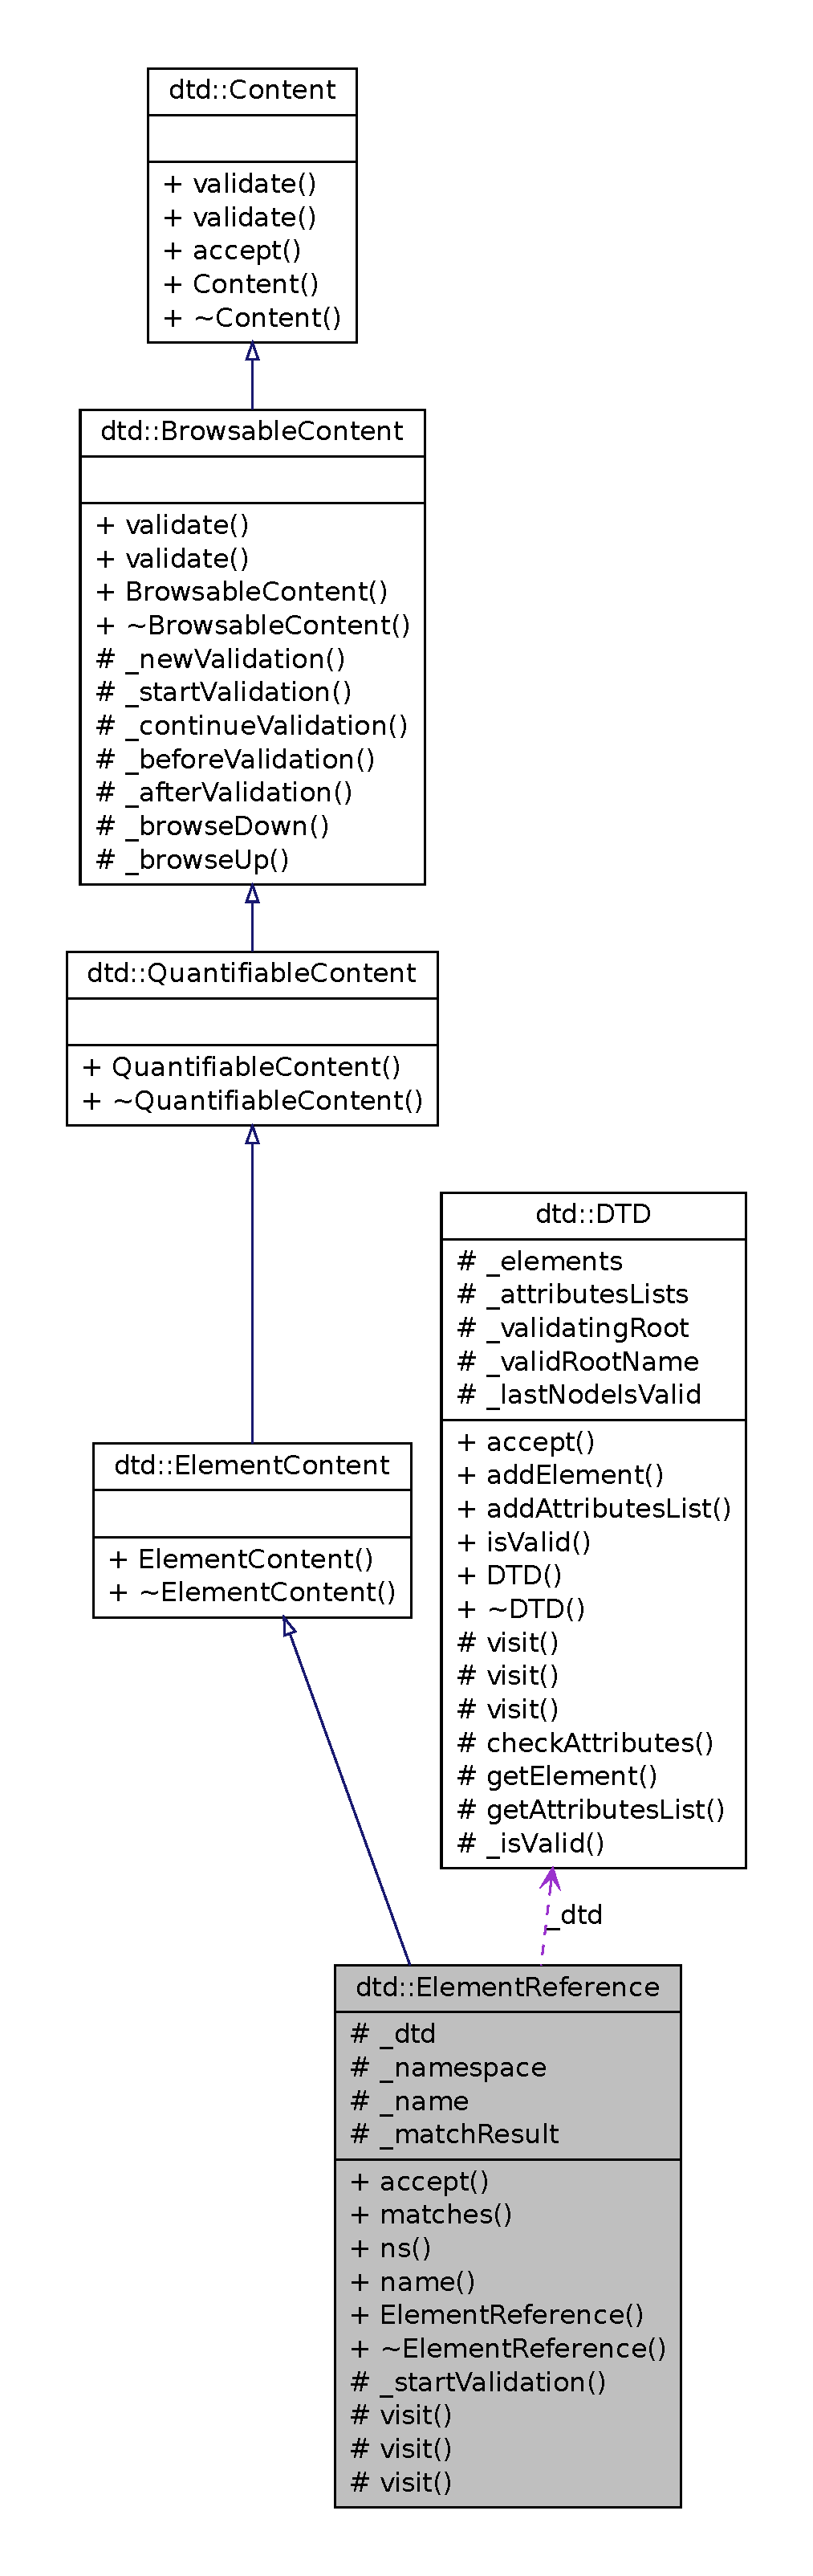
\includegraphics[height=600pt]{classdtd_1_1_element_reference__coll__graph}
\end{center}
\end{figure}
\subsection*{Fonctions membres publiques}
\begin{DoxyCompactItemize}
\item 
virtual void \hyperlink{classdtd_1_1_element_reference_ade77978609f7a872d73c9507057f12a6}{accept} (\hyperlink{classdtd_1_1_interface_d_t_d_visitor}{InterfaceDTDVisitor} \&visitor) const 
\item 
virtual bool \hyperlink{classdtd_1_1_element_reference_addbee5c126c3df5a509398343fe3d043}{matches} (xml::Node \&node)
\item 
virtual std::string \hyperlink{classdtd_1_1_element_reference_a24bcadd2a54f4195d84e583d8c2fc807}{ns} () const 
\item 
virtual std::string \hyperlink{classdtd_1_1_element_reference_aa478c58671bcfb2708364fb7dea35a29}{name} () const 
\item 
\hyperlink{classdtd_1_1_element_reference_a9b1697e8b813ba8214b028e2058bde8c}{ElementReference} (\hyperlink{classdtd_1_1_d_t_d}{DTD} \&dtd, std::string ns, std::string name)
\item 
virtual \hyperlink{classdtd_1_1_element_reference_ab95dafaf2cc11bafbd94ecc74f9f0c7f}{$\sim$ElementReference} ()
\end{DoxyCompactItemize}
\subsection*{Fonctions membres protégées}
\begin{DoxyCompactItemize}
\item 
virtual bool \hyperlink{classdtd_1_1_element_reference_a04d0141fbcfd0ff6171cd085c91e5622}{\_\-startValidation} (xml::CompositeMarkupNode::ChildrenIterator firstToken, xml::CompositeMarkupNode::ChildrenIterator endToken, \hyperlink{classdtd_1_1_browsable_content}{BrowsableContent} $\ast$nextStep)
\item 
virtual void \hyperlink{classdtd_1_1_element_reference_a4ffa8db697a0da84571c01623b9ab969}{visit} (const xml::TextNode \&node)
\item 
virtual void \hyperlink{classdtd_1_1_element_reference_aa983fa6f899fdfc9ad7769f5a479dce4}{visit} (const xml::MarkupNode \&node)
\item 
virtual void \hyperlink{classdtd_1_1_element_reference_a623d753307b938b9b29501bb96d9503d}{visit} (const xml::CompositeMarkupNode \&node)
\end{DoxyCompactItemize}
\subsection*{Attributs protégés}
\begin{DoxyCompactItemize}
\item 
\hyperlink{classdtd_1_1_d_t_d}{DTD} \& \hyperlink{classdtd_1_1_element_reference_a1aa135e9320d9117a70401d299ad04cb}{\_\-dtd}
\item 
std::string \hyperlink{classdtd_1_1_element_reference_ae290dc9372690c6ec326ee77594466ec}{\_\-namespace}
\item 
std::string \hyperlink{classdtd_1_1_element_reference_a3644697416e87370eedfa296d1c976ac}{\_\-name}
\item 
bool \hyperlink{classdtd_1_1_element_reference_ac8eea1ec6ad68e911179025d5471929b}{\_\-matchResult}
\end{DoxyCompactItemize}


\subsection{Description détaillée}


Définition à la ligne 22 du fichier ElementReference.hh.



\subsection{Documentation des constructeurs et destructeur}
\hypertarget{classdtd_1_1_element_reference_a9b1697e8b813ba8214b028e2058bde8c}{
\index{dtd::ElementReference@{dtd::ElementReference}!ElementReference@{ElementReference}}
\index{ElementReference@{ElementReference}!dtd::ElementReference@{dtd::ElementReference}}
\subsubsection[{ElementReference}]{\setlength{\rightskip}{0pt plus 5cm}dtd::ElementReference::ElementReference (
\begin{DoxyParamCaption}
\item[{{\bf DTD} \&}]{ dtd, }
\item[{std::string}]{ ns, }
\item[{std::string}]{ name}
\end{DoxyParamCaption}
)}}
\label{classdtd_1_1_element_reference_a9b1697e8b813ba8214b028e2058bde8c}


Définition à la ligne 62 du fichier ElementReference.cpp.

\hypertarget{classdtd_1_1_element_reference_ab95dafaf2cc11bafbd94ecc74f9f0c7f}{
\index{dtd::ElementReference@{dtd::ElementReference}!$\sim$ElementReference@{$\sim$ElementReference}}
\index{$\sim$ElementReference@{$\sim$ElementReference}!dtd::ElementReference@{dtd::ElementReference}}
\subsubsection[{$\sim$ElementReference}]{\setlength{\rightskip}{0pt plus 5cm}dtd::ElementReference::$\sim$ElementReference (
\begin{DoxyParamCaption}
{}
\end{DoxyParamCaption}
)\hspace{0.3cm}{\ttfamily  \mbox{[}virtual\mbox{]}}}}
\label{classdtd_1_1_element_reference_ab95dafaf2cc11bafbd94ecc74f9f0c7f}


Définition à la ligne 68 du fichier ElementReference.cpp.



\subsection{Documentation des fonctions membres}
\hypertarget{classdtd_1_1_element_reference_a04d0141fbcfd0ff6171cd085c91e5622}{
\index{dtd::ElementReference@{dtd::ElementReference}!\_\-startValidation@{\_\-startValidation}}
\index{\_\-startValidation@{\_\-startValidation}!dtd::ElementReference@{dtd::ElementReference}}
\subsubsection[{\_\-startValidation}]{\setlength{\rightskip}{0pt plus 5cm}virtual bool dtd::ElementReference::\_\-startValidation (
\begin{DoxyParamCaption}
\item[{xml::CompositeMarkupNode::ChildrenIterator}]{ firstToken, }
\item[{xml::CompositeMarkupNode::ChildrenIterator}]{ endToken, }
\item[{{\bf BrowsableContent} $\ast$}]{ nextStep}
\end{DoxyParamCaption}
)\hspace{0.3cm}{\ttfamily  \mbox{[}protected, virtual\mbox{]}}}}
\label{classdtd_1_1_element_reference_a04d0141fbcfd0ff6171cd085c91e5622}


Implémente \hyperlink{classdtd_1_1_browsable_content_a67ab5a7329d94e363796ae2d17617246}{dtd::BrowsableContent}.

\hypertarget{classdtd_1_1_element_reference_ade77978609f7a872d73c9507057f12a6}{
\index{dtd::ElementReference@{dtd::ElementReference}!accept@{accept}}
\index{accept@{accept}!dtd::ElementReference@{dtd::ElementReference}}
\subsubsection[{accept}]{\setlength{\rightskip}{0pt plus 5cm}void dtd::ElementReference::accept (
\begin{DoxyParamCaption}
\item[{{\bf InterfaceDTDVisitor} \&}]{ visitor}
\end{DoxyParamCaption}
) const\hspace{0.3cm}{\ttfamily  \mbox{[}virtual\mbox{]}}}}
\label{classdtd_1_1_element_reference_ade77978609f7a872d73c9507057f12a6}


Implémente \hyperlink{classdtd_1_1_content_a403cc15f12eaa187ad493fa600540cd8}{dtd::Content}.



Définition à la ligne 36 du fichier ElementReference.cpp.



Voici le graphe d'appel pour cette fonction :\nopagebreak
\begin{figure}[H]
\begin{center}
\leavevmode
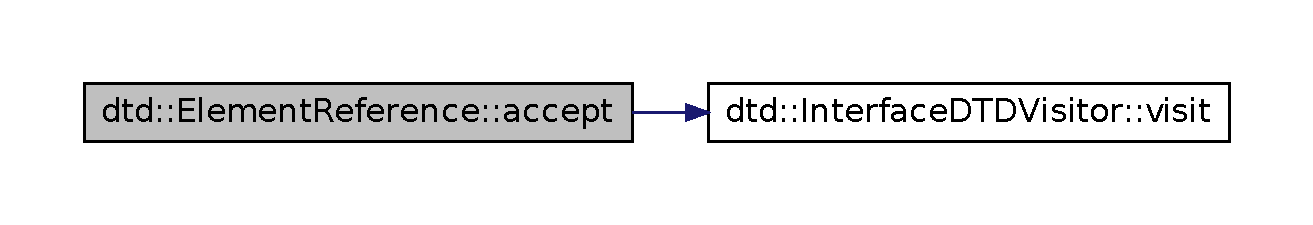
\includegraphics[width=400pt]{classdtd_1_1_element_reference_ade77978609f7a872d73c9507057f12a6_cgraph}
\end{center}
\end{figure}


\hypertarget{classdtd_1_1_element_reference_addbee5c126c3df5a509398343fe3d043}{
\index{dtd::ElementReference@{dtd::ElementReference}!matches@{matches}}
\index{matches@{matches}!dtd::ElementReference@{dtd::ElementReference}}
\subsubsection[{matches}]{\setlength{\rightskip}{0pt plus 5cm}bool dtd::ElementReference::matches (
\begin{DoxyParamCaption}
\item[{xml::Node \&}]{ node}
\end{DoxyParamCaption}
)\hspace{0.3cm}{\ttfamily  \mbox{[}virtual\mbox{]}}}}
\label{classdtd_1_1_element_reference_addbee5c126c3df5a509398343fe3d043}


Définition à la ligne 41 du fichier ElementReference.cpp.

\hypertarget{classdtd_1_1_element_reference_aa478c58671bcfb2708364fb7dea35a29}{
\index{dtd::ElementReference@{dtd::ElementReference}!name@{name}}
\index{name@{name}!dtd::ElementReference@{dtd::ElementReference}}
\subsubsection[{name}]{\setlength{\rightskip}{0pt plus 5cm}std::string dtd::ElementReference::name (
\begin{DoxyParamCaption}
{}
\end{DoxyParamCaption}
) const\hspace{0.3cm}{\ttfamily  \mbox{[}virtual\mbox{]}}}}
\label{classdtd_1_1_element_reference_aa478c58671bcfb2708364fb7dea35a29}


Définition à la ligne 53 du fichier ElementReference.cpp.

\hypertarget{classdtd_1_1_element_reference_a24bcadd2a54f4195d84e583d8c2fc807}{
\index{dtd::ElementReference@{dtd::ElementReference}!ns@{ns}}
\index{ns@{ns}!dtd::ElementReference@{dtd::ElementReference}}
\subsubsection[{ns}]{\setlength{\rightskip}{0pt plus 5cm}std::string dtd::ElementReference::ns (
\begin{DoxyParamCaption}
{}
\end{DoxyParamCaption}
) const\hspace{0.3cm}{\ttfamily  \mbox{[}virtual\mbox{]}}}}
\label{classdtd_1_1_element_reference_a24bcadd2a54f4195d84e583d8c2fc807}


Définition à la ligne 48 du fichier ElementReference.cpp.

\hypertarget{classdtd_1_1_element_reference_aa983fa6f899fdfc9ad7769f5a479dce4}{
\index{dtd::ElementReference@{dtd::ElementReference}!visit@{visit}}
\index{visit@{visit}!dtd::ElementReference@{dtd::ElementReference}}
\subsubsection[{visit}]{\setlength{\rightskip}{0pt plus 5cm}virtual void dtd::ElementReference::visit (
\begin{DoxyParamCaption}
\item[{const xml::MarkupNode \&}]{ node}
\end{DoxyParamCaption}
)\hspace{0.3cm}{\ttfamily  \mbox{[}protected, virtual\mbox{]}}}}
\label{classdtd_1_1_element_reference_aa983fa6f899fdfc9ad7769f5a479dce4}
\hypertarget{classdtd_1_1_element_reference_a623d753307b938b9b29501bb96d9503d}{
\index{dtd::ElementReference@{dtd::ElementReference}!visit@{visit}}
\index{visit@{visit}!dtd::ElementReference@{dtd::ElementReference}}
\subsubsection[{visit}]{\setlength{\rightskip}{0pt plus 5cm}virtual void dtd::ElementReference::visit (
\begin{DoxyParamCaption}
\item[{const xml::CompositeMarkupNode \&}]{ node}
\end{DoxyParamCaption}
)\hspace{0.3cm}{\ttfamily  \mbox{[}protected, virtual\mbox{]}}}}
\label{classdtd_1_1_element_reference_a623d753307b938b9b29501bb96d9503d}
\hypertarget{classdtd_1_1_element_reference_a4ffa8db697a0da84571c01623b9ab969}{
\index{dtd::ElementReference@{dtd::ElementReference}!visit@{visit}}
\index{visit@{visit}!dtd::ElementReference@{dtd::ElementReference}}
\subsubsection[{visit}]{\setlength{\rightskip}{0pt plus 5cm}virtual void dtd::ElementReference::visit (
\begin{DoxyParamCaption}
\item[{const xml::TextNode \&}]{ node}
\end{DoxyParamCaption}
)\hspace{0.3cm}{\ttfamily  \mbox{[}protected, virtual\mbox{]}}}}
\label{classdtd_1_1_element_reference_a4ffa8db697a0da84571c01623b9ab969}


\subsection{Documentation des données membres}
\hypertarget{classdtd_1_1_element_reference_a1aa135e9320d9117a70401d299ad04cb}{
\index{dtd::ElementReference@{dtd::ElementReference}!\_\-dtd@{\_\-dtd}}
\index{\_\-dtd@{\_\-dtd}!dtd::ElementReference@{dtd::ElementReference}}
\subsubsection[{\_\-dtd}]{\setlength{\rightskip}{0pt plus 5cm}{\bf DTD}\& {\bf dtd::ElementReference::\_\-dtd}\hspace{0.3cm}{\ttfamily  \mbox{[}protected\mbox{]}}}}
\label{classdtd_1_1_element_reference_a1aa135e9320d9117a70401d299ad04cb}


Définition à la ligne 54 du fichier ElementReference.hh.

\hypertarget{classdtd_1_1_element_reference_ac8eea1ec6ad68e911179025d5471929b}{
\index{dtd::ElementReference@{dtd::ElementReference}!\_\-matchResult@{\_\-matchResult}}
\index{\_\-matchResult@{\_\-matchResult}!dtd::ElementReference@{dtd::ElementReference}}
\subsubsection[{\_\-matchResult}]{\setlength{\rightskip}{0pt plus 5cm}bool {\bf dtd::ElementReference::\_\-matchResult}\hspace{0.3cm}{\ttfamily  \mbox{[}protected\mbox{]}}}}
\label{classdtd_1_1_element_reference_ac8eea1ec6ad68e911179025d5471929b}


Définition à la ligne 58 du fichier ElementReference.hh.

\hypertarget{classdtd_1_1_element_reference_a3644697416e87370eedfa296d1c976ac}{
\index{dtd::ElementReference@{dtd::ElementReference}!\_\-name@{\_\-name}}
\index{\_\-name@{\_\-name}!dtd::ElementReference@{dtd::ElementReference}}
\subsubsection[{\_\-name}]{\setlength{\rightskip}{0pt plus 5cm}std::string {\bf dtd::ElementReference::\_\-name}\hspace{0.3cm}{\ttfamily  \mbox{[}protected\mbox{]}}}}
\label{classdtd_1_1_element_reference_a3644697416e87370eedfa296d1c976ac}


Définition à la ligne 56 du fichier ElementReference.hh.

\hypertarget{classdtd_1_1_element_reference_ae290dc9372690c6ec326ee77594466ec}{
\index{dtd::ElementReference@{dtd::ElementReference}!\_\-namespace@{\_\-namespace}}
\index{\_\-namespace@{\_\-namespace}!dtd::ElementReference@{dtd::ElementReference}}
\subsubsection[{\_\-namespace}]{\setlength{\rightskip}{0pt plus 5cm}std::string {\bf dtd::ElementReference::\_\-namespace}\hspace{0.3cm}{\ttfamily  \mbox{[}protected\mbox{]}}}}
\label{classdtd_1_1_element_reference_ae290dc9372690c6ec326ee77594466ec}


Définition à la ligne 55 du fichier ElementReference.hh.



La documentation de cette classe a été générée à partir des fichiers suivants :\begin{DoxyCompactItemize}
\item 
src/\hyperlink{_element_reference_8hh}{ElementReference.hh}\item 
src/\hyperlink{_element_reference_8cpp}{ElementReference.cpp}\end{DoxyCompactItemize}

\hypertarget{classdtd_1_1_empty_content}{
\section{Référence de la classe dtd::EmptyContent}
\label{classdtd_1_1_empty_content}\index{dtd::EmptyContent@{dtd::EmptyContent}}
}


{\ttfamily \#include $<$EmptyContent.hh$>$}



Graphe d'héritage de dtd::EmptyContent:\nopagebreak
\begin{figure}[H]
\begin{center}
\leavevmode
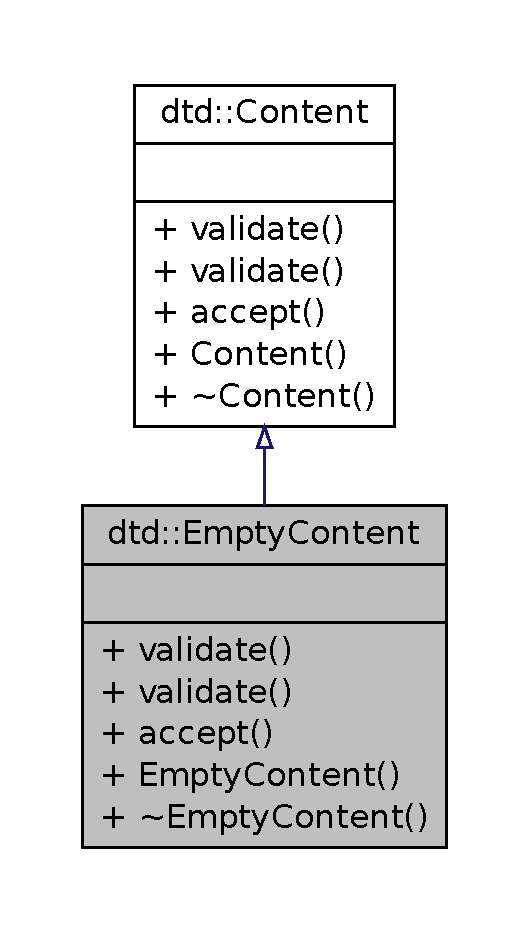
\includegraphics[width=254pt]{classdtd_1_1_empty_content__inherit__graph}
\end{center}
\end{figure}


Graphe de collaboration de dtd::EmptyContent:\nopagebreak
\begin{figure}[H]
\begin{center}
\leavevmode
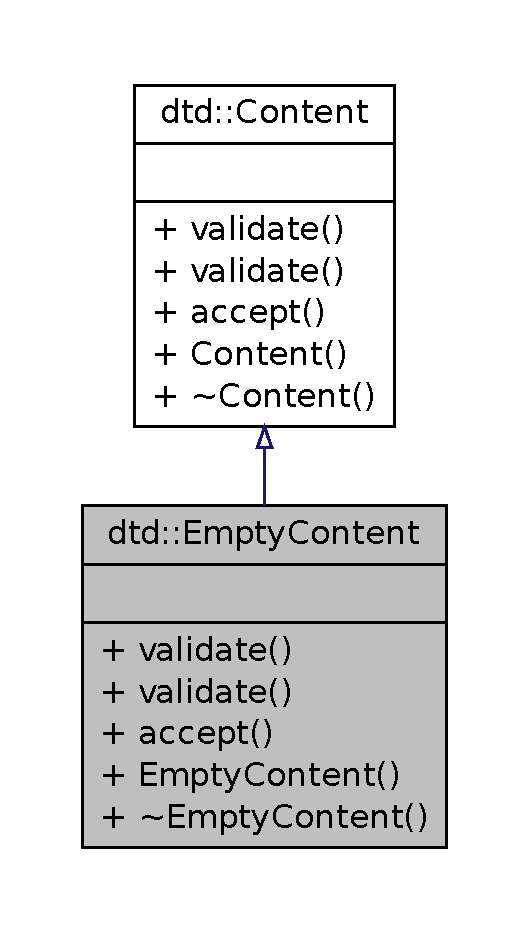
\includegraphics[width=254pt]{classdtd_1_1_empty_content__coll__graph}
\end{center}
\end{figure}
\subsection*{Fonctions membres publiques}
\begin{DoxyCompactItemize}
\item 
virtual bool \hyperlink{classdtd_1_1_empty_content_a763480d5964b94051f15a7ee5fbb936b}{validate} (const xml::MarkupNode \&node)
\item 
virtual bool \hyperlink{classdtd_1_1_empty_content_a97da0ccd8f6156b168f13759c920c6cc}{validate} (const xml::CompositeMarkupNode \&node)
\item 
virtual void \hyperlink{classdtd_1_1_empty_content_a8440fe4e357b401e8db8d05baf59803e}{accept} (\hyperlink{classdtd_1_1_interface_d_t_d_visitor}{InterfaceDTDVisitor} \&visitor) const 
\item 
\hyperlink{classdtd_1_1_empty_content_a81e2a7171e15447fa33a5b473073ffff}{EmptyContent} ()
\item 
virtual \hyperlink{classdtd_1_1_empty_content_a35b3bed652050e8e7aced4482bfc25d7}{$\sim$EmptyContent} ()
\end{DoxyCompactItemize}


\subsection{Description détaillée}


Définition à la ligne 17 du fichier EmptyContent.hh.



\subsection{Documentation des constructeurs et destructeur}
\hypertarget{classdtd_1_1_empty_content_a81e2a7171e15447fa33a5b473073ffff}{
\index{dtd::EmptyContent@{dtd::EmptyContent}!EmptyContent@{EmptyContent}}
\index{EmptyContent@{EmptyContent}!dtd::EmptyContent@{dtd::EmptyContent}}
\subsubsection[{EmptyContent}]{\setlength{\rightskip}{0pt plus 5cm}dtd::EmptyContent::EmptyContent (
\begin{DoxyParamCaption}
{}
\end{DoxyParamCaption}
)}}
\label{classdtd_1_1_empty_content_a81e2a7171e15447fa33a5b473073ffff}


Définition à la ligne 52 du fichier EmptyContent.cpp.

\hypertarget{classdtd_1_1_empty_content_a35b3bed652050e8e7aced4482bfc25d7}{
\index{dtd::EmptyContent@{dtd::EmptyContent}!$\sim$EmptyContent@{$\sim$EmptyContent}}
\index{$\sim$EmptyContent@{$\sim$EmptyContent}!dtd::EmptyContent@{dtd::EmptyContent}}
\subsubsection[{$\sim$EmptyContent}]{\setlength{\rightskip}{0pt plus 5cm}dtd::EmptyContent::$\sim$EmptyContent (
\begin{DoxyParamCaption}
{}
\end{DoxyParamCaption}
)\hspace{0.3cm}{\ttfamily  \mbox{[}virtual\mbox{]}}}}
\label{classdtd_1_1_empty_content_a35b3bed652050e8e7aced4482bfc25d7}


Définition à la ligne 57 du fichier EmptyContent.cpp.



\subsection{Documentation des fonctions membres}
\hypertarget{classdtd_1_1_empty_content_a8440fe4e357b401e8db8d05baf59803e}{
\index{dtd::EmptyContent@{dtd::EmptyContent}!accept@{accept}}
\index{accept@{accept}!dtd::EmptyContent@{dtd::EmptyContent}}
\subsubsection[{accept}]{\setlength{\rightskip}{0pt plus 5cm}void dtd::EmptyContent::accept (
\begin{DoxyParamCaption}
\item[{{\bf InterfaceDTDVisitor} \&}]{ visitor}
\end{DoxyParamCaption}
) const\hspace{0.3cm}{\ttfamily  \mbox{[}virtual\mbox{]}}}}
\label{classdtd_1_1_empty_content_a8440fe4e357b401e8db8d05baf59803e}


Implémente \hyperlink{classdtd_1_1_content_a403cc15f12eaa187ad493fa600540cd8}{dtd::Content}.



Définition à la ligne 43 du fichier EmptyContent.cpp.



Voici le graphe d'appel pour cette fonction :\nopagebreak
\begin{figure}[H]
\begin{center}
\leavevmode
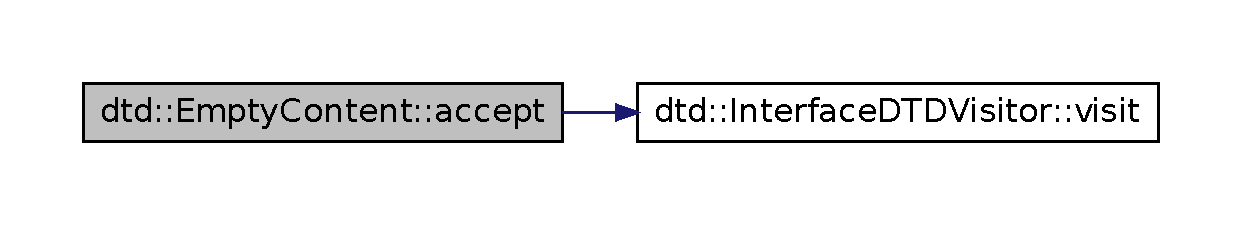
\includegraphics[width=400pt]{classdtd_1_1_empty_content_a8440fe4e357b401e8db8d05baf59803e_cgraph}
\end{center}
\end{figure}


\hypertarget{classdtd_1_1_empty_content_a763480d5964b94051f15a7ee5fbb936b}{
\index{dtd::EmptyContent@{dtd::EmptyContent}!validate@{validate}}
\index{validate@{validate}!dtd::EmptyContent@{dtd::EmptyContent}}
\subsubsection[{validate}]{\setlength{\rightskip}{0pt plus 5cm}virtual bool dtd::EmptyContent::validate (
\begin{DoxyParamCaption}
\item[{const xml::MarkupNode \&}]{ node}
\end{DoxyParamCaption}
)\hspace{0.3cm}{\ttfamily  \mbox{[}virtual\mbox{]}}}}
\label{classdtd_1_1_empty_content_a763480d5964b94051f15a7ee5fbb936b}


Implémente \hyperlink{classdtd_1_1_content_a2095fb10a09f6767aaf5e6da4b3018f1}{dtd::Content}.

\hypertarget{classdtd_1_1_empty_content_a97da0ccd8f6156b168f13759c920c6cc}{
\index{dtd::EmptyContent@{dtd::EmptyContent}!validate@{validate}}
\index{validate@{validate}!dtd::EmptyContent@{dtd::EmptyContent}}
\subsubsection[{validate}]{\setlength{\rightskip}{0pt plus 5cm}virtual bool dtd::EmptyContent::validate (
\begin{DoxyParamCaption}
\item[{const xml::CompositeMarkupNode \&}]{ node}
\end{DoxyParamCaption}
)\hspace{0.3cm}{\ttfamily  \mbox{[}virtual\mbox{]}}}}
\label{classdtd_1_1_empty_content_a97da0ccd8f6156b168f13759c920c6cc}


Implémente \hyperlink{classdtd_1_1_content_acaa15daa3a3a2cf11632c4c93dc2cf37}{dtd::Content}.



La documentation de cette classe a été générée à partir des fichiers suivants :\begin{DoxyCompactItemize}
\item 
src/\hyperlink{_empty_content_8hh}{EmptyContent.hh}\item 
src/\hyperlink{_empty_content_8cpp}{EmptyContent.cpp}\end{DoxyCompactItemize}

\hypertarget{classdtd_1_1_interface_d_t_d_visitor}{
\section{Référence de la classe dtd::InterfaceDTDVisitor}
\label{classdtd_1_1_interface_d_t_d_visitor}\index{dtd::InterfaceDTDVisitor@{dtd::InterfaceDTDVisitor}}
}


{\ttfamily \#include $<$InterfaceDTDVisitor.hpp$>$}



Graphe d'héritage de dtd::InterfaceDTDVisitor:\nopagebreak
\begin{figure}[H]
\begin{center}
\leavevmode
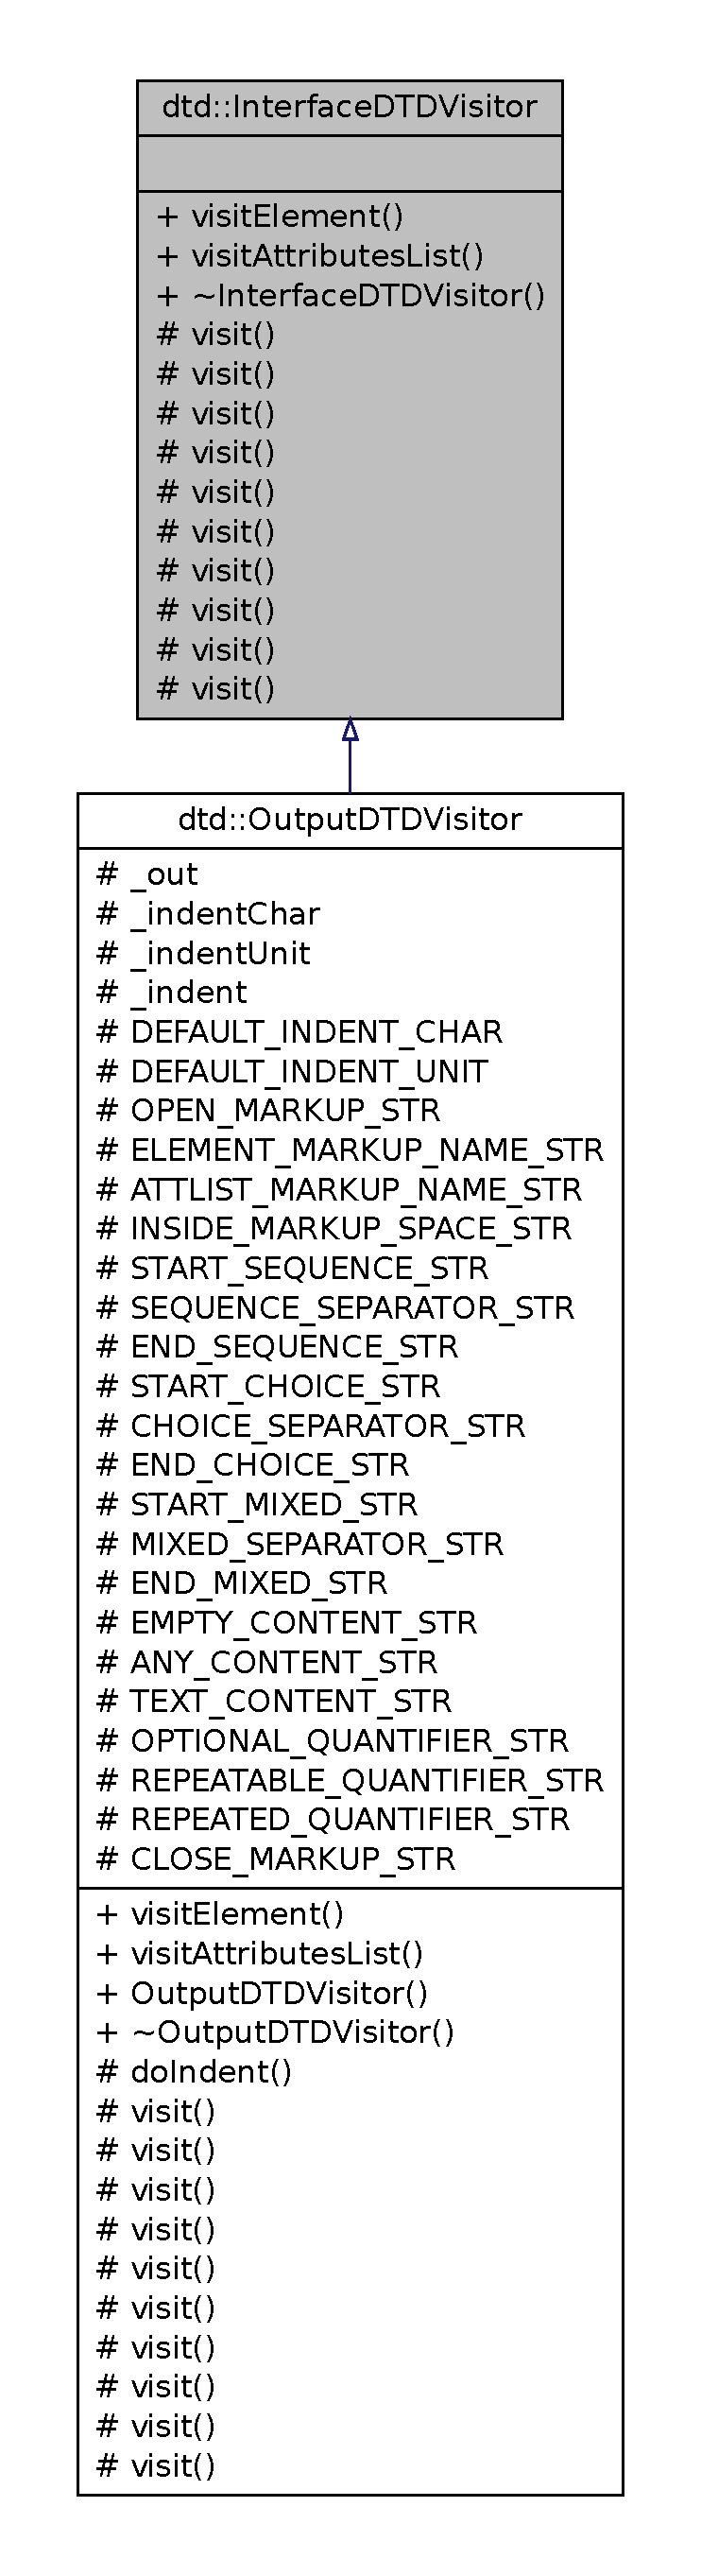
\includegraphics[height=600pt]{classdtd_1_1_interface_d_t_d_visitor__inherit__graph}
\end{center}
\end{figure}
\subsection*{Fonctions membres publiques}
\begin{DoxyCompactItemize}
\item 
virtual void \hyperlink{classdtd_1_1_interface_d_t_d_visitor_a46b882a06961ea04fd43b2a9d937118b}{visitElement} (const std::string \&ns, const std::string \&elementName, const \hyperlink{classdtd_1_1_content}{Content} \&content)=0
\item 
virtual void \hyperlink{classdtd_1_1_interface_d_t_d_visitor_a729d9fcb360d9bf45210aac109b388da}{visitAttributesList} (const std::string \&ns, const std::string \&elementName, const \hyperlink{namespacedtd_a8d5d29abb5de0468925f321597f57f4b}{AttributesList} \&attlist)=0
\item 
virtual \hyperlink{classdtd_1_1_interface_d_t_d_visitor_aef94cba5e56a7891a24b236176a2075a}{$\sim$InterfaceDTDVisitor} ()
\end{DoxyCompactItemize}
\subsection*{Fonctions membres protégées}
\begin{DoxyCompactItemize}
\item 
virtual void \hyperlink{classdtd_1_1_interface_d_t_d_visitor_ac2d1f472564e590bbe66f14ab096167a}{visit} (const \hyperlink{classdtd_1_1_any_content}{AnyContent} \&content)=0
\item 
virtual void \hyperlink{classdtd_1_1_interface_d_t_d_visitor_abdf03eb698f07aa0caaa405711fc8aac}{visit} (const \hyperlink{classdtd_1_1_empty_content}{EmptyContent} \&content)=0
\item 
virtual void \hyperlink{classdtd_1_1_interface_d_t_d_visitor_a06be244faf5995ac7ca502b326db10e0}{visit} (const \hyperlink{classdtd_1_1_mixed_content}{MixedContent} \&content)=0
\item 
virtual void \hyperlink{classdtd_1_1_interface_d_t_d_visitor_abd31e761d6d8ab80ac6f3f0a9a20b953}{visit} (const \hyperlink{classdtd_1_1_text_content}{TextContent} \&content)=0
\item 
virtual void \hyperlink{classdtd_1_1_interface_d_t_d_visitor_aaac54822c9519b08305a64aab110716b}{visit} (const \hyperlink{classdtd_1_1_element_reference}{ElementReference} \&element)=0
\item 
virtual void \hyperlink{classdtd_1_1_interface_d_t_d_visitor_a4323aeef86fa385a44fd4572ccc36cd2}{visit} (const \hyperlink{classdtd_1_1_choice}{Choice} \&content)=0
\item 
virtual void \hyperlink{classdtd_1_1_interface_d_t_d_visitor_aa093199d020b5887fbaa8af1573afc51}{visit} (const \hyperlink{classdtd_1_1_sequence}{Sequence} \&content)=0
\item 
virtual void \hyperlink{classdtd_1_1_interface_d_t_d_visitor_a444ada6db2f531579579de7b8fd5fd53}{visit} (const \hyperlink{classdtd_1_1_optional_content}{OptionalContent} \&content)=0
\item 
virtual void \hyperlink{classdtd_1_1_interface_d_t_d_visitor_a76bd6fb0307eea7fc6ef703cf09a07b9}{visit} (const \hyperlink{classdtd_1_1_repeatable_content}{RepeatableContent} \&content)=0
\item 
virtual void \hyperlink{classdtd_1_1_interface_d_t_d_visitor_a8a2ce739049697fcc2a7126adea4536a}{visit} (const \hyperlink{classdtd_1_1_repeated_content}{RepeatedContent} \&content)=0
\end{DoxyCompactItemize}
\subsection*{Amis}
\begin{DoxyCompactItemize}
\item 
class \hyperlink{classdtd_1_1_interface_d_t_d_visitor_a98eaefc8d4a0da1a8f9c254c62a68759}{AnyContent}
\item 
class \hyperlink{classdtd_1_1_interface_d_t_d_visitor_a91eaa900fb18be6cd9a7105c964666fb}{EmptyContent}
\item 
class \hyperlink{classdtd_1_1_interface_d_t_d_visitor_a94c4de9fad580ef7aa4f384bf0c2b861}{MixedContent}
\item 
class \hyperlink{classdtd_1_1_interface_d_t_d_visitor_aa641efa971cba38c6181cdc71b30df90}{TextContent}
\item 
class \hyperlink{classdtd_1_1_interface_d_t_d_visitor_a21b7004458ebe5b88f6d6edb6d059a34}{ElementReference}
\item 
class \hyperlink{classdtd_1_1_interface_d_t_d_visitor_af8084f88f5641132057732496deab026}{Choice}
\item 
class \hyperlink{classdtd_1_1_interface_d_t_d_visitor_a26271d5afaff6e6d3f00c055c63d0b24}{Sequence}
\item 
class \hyperlink{classdtd_1_1_interface_d_t_d_visitor_a90839fb65068433fb68ba4e59462f869}{OptionalContent}
\item 
class \hyperlink{classdtd_1_1_interface_d_t_d_visitor_ad2e096c883291671a8d20ca270018e05}{RepeatableContent}
\item 
class \hyperlink{classdtd_1_1_interface_d_t_d_visitor_afaa2f3eab18d4215d1683c4b2f5a6b8e}{RepeatedContent}
\end{DoxyCompactItemize}


\subsection{Description détaillée}


Définition à la ligne 30 du fichier InterfaceDTDVisitor.hpp.



\subsection{Documentation des constructeurs et destructeur}
\hypertarget{classdtd_1_1_interface_d_t_d_visitor_aef94cba5e56a7891a24b236176a2075a}{
\index{dtd::InterfaceDTDVisitor@{dtd::InterfaceDTDVisitor}!$\sim$InterfaceDTDVisitor@{$\sim$InterfaceDTDVisitor}}
\index{$\sim$InterfaceDTDVisitor@{$\sim$InterfaceDTDVisitor}!dtd::InterfaceDTDVisitor@{dtd::InterfaceDTDVisitor}}
\subsubsection[{$\sim$InterfaceDTDVisitor}]{\setlength{\rightskip}{0pt plus 5cm}virtual dtd::InterfaceDTDVisitor::$\sim$InterfaceDTDVisitor (
\begin{DoxyParamCaption}
{}
\end{DoxyParamCaption}
)\hspace{0.3cm}{\ttfamily  \mbox{[}inline, virtual\mbox{]}}}}
\label{classdtd_1_1_interface_d_t_d_visitor_aef94cba5e56a7891a24b236176a2075a}


Définition à la ligne 46 du fichier InterfaceDTDVisitor.hpp.



\subsection{Documentation des fonctions membres}
\hypertarget{classdtd_1_1_interface_d_t_d_visitor_ac2d1f472564e590bbe66f14ab096167a}{
\index{dtd::InterfaceDTDVisitor@{dtd::InterfaceDTDVisitor}!visit@{visit}}
\index{visit@{visit}!dtd::InterfaceDTDVisitor@{dtd::InterfaceDTDVisitor}}
\subsubsection[{visit}]{\setlength{\rightskip}{0pt plus 5cm}virtual void dtd::InterfaceDTDVisitor::visit (
\begin{DoxyParamCaption}
\item[{const {\bf AnyContent} \&}]{ content}
\end{DoxyParamCaption}
)\hspace{0.3cm}{\ttfamily  \mbox{[}protected, pure virtual\mbox{]}}}}
\label{classdtd_1_1_interface_d_t_d_visitor_ac2d1f472564e590bbe66f14ab096167a}


Implémenté dans \hyperlink{classdtd_1_1_output_d_t_d_visitor_a17406ea51970e67da79947709945c4b1}{dtd::OutputDTDVisitor}.



Voici le graphe d'appel pour cette fonction :\nopagebreak
\begin{figure}[H]
\begin{center}
\leavevmode
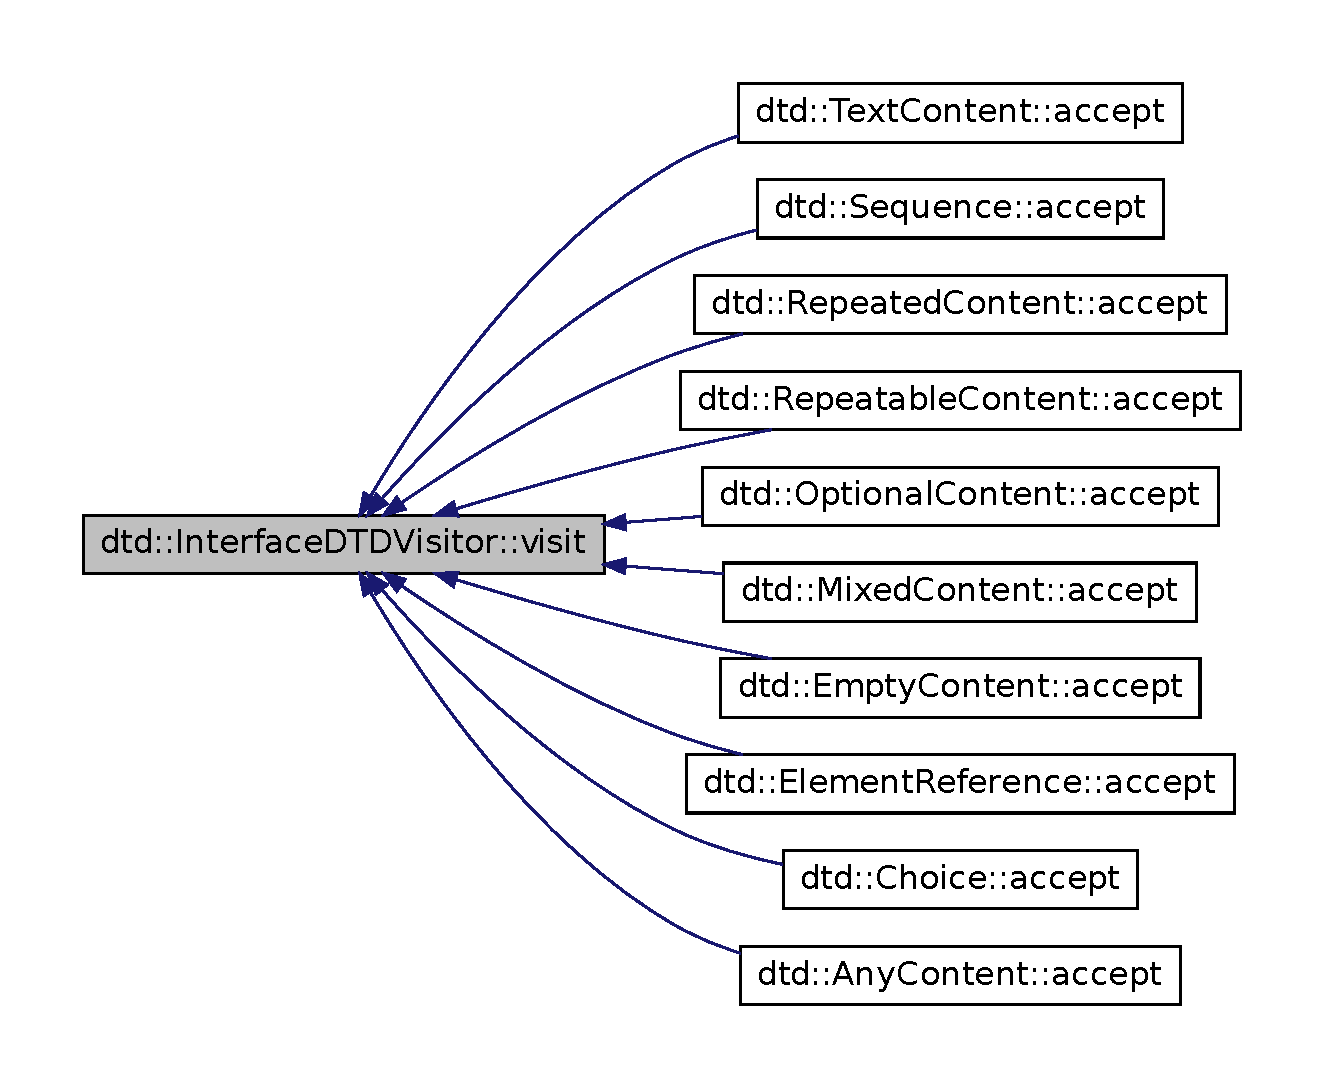
\includegraphics[width=400pt]{classdtd_1_1_interface_d_t_d_visitor_ac2d1f472564e590bbe66f14ab096167a_icgraph}
\end{center}
\end{figure}


\hypertarget{classdtd_1_1_interface_d_t_d_visitor_abdf03eb698f07aa0caaa405711fc8aac}{
\index{dtd::InterfaceDTDVisitor@{dtd::InterfaceDTDVisitor}!visit@{visit}}
\index{visit@{visit}!dtd::InterfaceDTDVisitor@{dtd::InterfaceDTDVisitor}}
\subsubsection[{visit}]{\setlength{\rightskip}{0pt plus 5cm}virtual void dtd::InterfaceDTDVisitor::visit (
\begin{DoxyParamCaption}
\item[{const {\bf EmptyContent} \&}]{ content}
\end{DoxyParamCaption}
)\hspace{0.3cm}{\ttfamily  \mbox{[}protected, pure virtual\mbox{]}}}}
\label{classdtd_1_1_interface_d_t_d_visitor_abdf03eb698f07aa0caaa405711fc8aac}


Implémenté dans \hyperlink{classdtd_1_1_output_d_t_d_visitor_a3eb81ed67c53e9aebb90a4558f13a402}{dtd::OutputDTDVisitor}.

\hypertarget{classdtd_1_1_interface_d_t_d_visitor_a76bd6fb0307eea7fc6ef703cf09a07b9}{
\index{dtd::InterfaceDTDVisitor@{dtd::InterfaceDTDVisitor}!visit@{visit}}
\index{visit@{visit}!dtd::InterfaceDTDVisitor@{dtd::InterfaceDTDVisitor}}
\subsubsection[{visit}]{\setlength{\rightskip}{0pt plus 5cm}virtual void dtd::InterfaceDTDVisitor::visit (
\begin{DoxyParamCaption}
\item[{const {\bf RepeatableContent} \&}]{ content}
\end{DoxyParamCaption}
)\hspace{0.3cm}{\ttfamily  \mbox{[}protected, pure virtual\mbox{]}}}}
\label{classdtd_1_1_interface_d_t_d_visitor_a76bd6fb0307eea7fc6ef703cf09a07b9}


Implémenté dans \hyperlink{classdtd_1_1_output_d_t_d_visitor_a93c6d6c010e58356bf9ba29b56d561df}{dtd::OutputDTDVisitor}.

\hypertarget{classdtd_1_1_interface_d_t_d_visitor_a444ada6db2f531579579de7b8fd5fd53}{
\index{dtd::InterfaceDTDVisitor@{dtd::InterfaceDTDVisitor}!visit@{visit}}
\index{visit@{visit}!dtd::InterfaceDTDVisitor@{dtd::InterfaceDTDVisitor}}
\subsubsection[{visit}]{\setlength{\rightskip}{0pt plus 5cm}virtual void dtd::InterfaceDTDVisitor::visit (
\begin{DoxyParamCaption}
\item[{const {\bf OptionalContent} \&}]{ content}
\end{DoxyParamCaption}
)\hspace{0.3cm}{\ttfamily  \mbox{[}protected, pure virtual\mbox{]}}}}
\label{classdtd_1_1_interface_d_t_d_visitor_a444ada6db2f531579579de7b8fd5fd53}


Implémenté dans \hyperlink{classdtd_1_1_output_d_t_d_visitor_a5ea91964e78eef4fc0786708154204bc}{dtd::OutputDTDVisitor}.

\hypertarget{classdtd_1_1_interface_d_t_d_visitor_a4323aeef86fa385a44fd4572ccc36cd2}{
\index{dtd::InterfaceDTDVisitor@{dtd::InterfaceDTDVisitor}!visit@{visit}}
\index{visit@{visit}!dtd::InterfaceDTDVisitor@{dtd::InterfaceDTDVisitor}}
\subsubsection[{visit}]{\setlength{\rightskip}{0pt plus 5cm}virtual void dtd::InterfaceDTDVisitor::visit (
\begin{DoxyParamCaption}
\item[{const {\bf Choice} \&}]{ content}
\end{DoxyParamCaption}
)\hspace{0.3cm}{\ttfamily  \mbox{[}protected, pure virtual\mbox{]}}}}
\label{classdtd_1_1_interface_d_t_d_visitor_a4323aeef86fa385a44fd4572ccc36cd2}


Implémenté dans \hyperlink{classdtd_1_1_output_d_t_d_visitor_a666c828c10840930fd420e86030e16f1}{dtd::OutputDTDVisitor}.

\hypertarget{classdtd_1_1_interface_d_t_d_visitor_aa093199d020b5887fbaa8af1573afc51}{
\index{dtd::InterfaceDTDVisitor@{dtd::InterfaceDTDVisitor}!visit@{visit}}
\index{visit@{visit}!dtd::InterfaceDTDVisitor@{dtd::InterfaceDTDVisitor}}
\subsubsection[{visit}]{\setlength{\rightskip}{0pt plus 5cm}virtual void dtd::InterfaceDTDVisitor::visit (
\begin{DoxyParamCaption}
\item[{const {\bf Sequence} \&}]{ content}
\end{DoxyParamCaption}
)\hspace{0.3cm}{\ttfamily  \mbox{[}protected, pure virtual\mbox{]}}}}
\label{classdtd_1_1_interface_d_t_d_visitor_aa093199d020b5887fbaa8af1573afc51}


Implémenté dans \hyperlink{classdtd_1_1_output_d_t_d_visitor_a5b9434224d99c416da826a88cd11df3f}{dtd::OutputDTDVisitor}.

\hypertarget{classdtd_1_1_interface_d_t_d_visitor_aaac54822c9519b08305a64aab110716b}{
\index{dtd::InterfaceDTDVisitor@{dtd::InterfaceDTDVisitor}!visit@{visit}}
\index{visit@{visit}!dtd::InterfaceDTDVisitor@{dtd::InterfaceDTDVisitor}}
\subsubsection[{visit}]{\setlength{\rightskip}{0pt plus 5cm}virtual void dtd::InterfaceDTDVisitor::visit (
\begin{DoxyParamCaption}
\item[{const {\bf ElementReference} \&}]{ element}
\end{DoxyParamCaption}
)\hspace{0.3cm}{\ttfamily  \mbox{[}protected, pure virtual\mbox{]}}}}
\label{classdtd_1_1_interface_d_t_d_visitor_aaac54822c9519b08305a64aab110716b}


Implémenté dans \hyperlink{classdtd_1_1_output_d_t_d_visitor_a4b286b6b0ca83035e25cef1ba6f10c47}{dtd::OutputDTDVisitor}.

\hypertarget{classdtd_1_1_interface_d_t_d_visitor_a8a2ce739049697fcc2a7126adea4536a}{
\index{dtd::InterfaceDTDVisitor@{dtd::InterfaceDTDVisitor}!visit@{visit}}
\index{visit@{visit}!dtd::InterfaceDTDVisitor@{dtd::InterfaceDTDVisitor}}
\subsubsection[{visit}]{\setlength{\rightskip}{0pt plus 5cm}virtual void dtd::InterfaceDTDVisitor::visit (
\begin{DoxyParamCaption}
\item[{const {\bf RepeatedContent} \&}]{ content}
\end{DoxyParamCaption}
)\hspace{0.3cm}{\ttfamily  \mbox{[}protected, pure virtual\mbox{]}}}}
\label{classdtd_1_1_interface_d_t_d_visitor_a8a2ce739049697fcc2a7126adea4536a}


Implémenté dans \hyperlink{classdtd_1_1_output_d_t_d_visitor_a01a2c44557480982c2ca5d3769e72c00}{dtd::OutputDTDVisitor}.

\hypertarget{classdtd_1_1_interface_d_t_d_visitor_a06be244faf5995ac7ca502b326db10e0}{
\index{dtd::InterfaceDTDVisitor@{dtd::InterfaceDTDVisitor}!visit@{visit}}
\index{visit@{visit}!dtd::InterfaceDTDVisitor@{dtd::InterfaceDTDVisitor}}
\subsubsection[{visit}]{\setlength{\rightskip}{0pt plus 5cm}virtual void dtd::InterfaceDTDVisitor::visit (
\begin{DoxyParamCaption}
\item[{const {\bf MixedContent} \&}]{ content}
\end{DoxyParamCaption}
)\hspace{0.3cm}{\ttfamily  \mbox{[}protected, pure virtual\mbox{]}}}}
\label{classdtd_1_1_interface_d_t_d_visitor_a06be244faf5995ac7ca502b326db10e0}


Implémenté dans \hyperlink{classdtd_1_1_output_d_t_d_visitor_a47692e383524d7804a6f5bf4d3f229b8}{dtd::OutputDTDVisitor}.

\hypertarget{classdtd_1_1_interface_d_t_d_visitor_abd31e761d6d8ab80ac6f3f0a9a20b953}{
\index{dtd::InterfaceDTDVisitor@{dtd::InterfaceDTDVisitor}!visit@{visit}}
\index{visit@{visit}!dtd::InterfaceDTDVisitor@{dtd::InterfaceDTDVisitor}}
\subsubsection[{visit}]{\setlength{\rightskip}{0pt plus 5cm}virtual void dtd::InterfaceDTDVisitor::visit (
\begin{DoxyParamCaption}
\item[{const {\bf TextContent} \&}]{ content}
\end{DoxyParamCaption}
)\hspace{0.3cm}{\ttfamily  \mbox{[}protected, pure virtual\mbox{]}}}}
\label{classdtd_1_1_interface_d_t_d_visitor_abd31e761d6d8ab80ac6f3f0a9a20b953}


Implémenté dans \hyperlink{classdtd_1_1_output_d_t_d_visitor_ad06e4a71ec8f36d91d59eb24ddc51f70}{dtd::OutputDTDVisitor}.

\hypertarget{classdtd_1_1_interface_d_t_d_visitor_a729d9fcb360d9bf45210aac109b388da}{
\index{dtd::InterfaceDTDVisitor@{dtd::InterfaceDTDVisitor}!visitAttributesList@{visitAttributesList}}
\index{visitAttributesList@{visitAttributesList}!dtd::InterfaceDTDVisitor@{dtd::InterfaceDTDVisitor}}
\subsubsection[{visitAttributesList}]{\setlength{\rightskip}{0pt plus 5cm}virtual void dtd::InterfaceDTDVisitor::visitAttributesList (
\begin{DoxyParamCaption}
\item[{const std::string \&}]{ ns, }
\item[{const std::string \&}]{ elementName, }
\item[{const {\bf AttributesList} \&}]{ attlist}
\end{DoxyParamCaption}
)\hspace{0.3cm}{\ttfamily  \mbox{[}pure virtual\mbox{]}}}}
\label{classdtd_1_1_interface_d_t_d_visitor_a729d9fcb360d9bf45210aac109b388da}


Implémenté dans \hyperlink{classdtd_1_1_output_d_t_d_visitor_aa1b6474bd068eca43a6eb61e90ff7504}{dtd::OutputDTDVisitor}.



Voici le graphe d'appel pour cette fonction :
\nopagebreak
\begin{figure}[H]
\begin{center}
\leavevmode
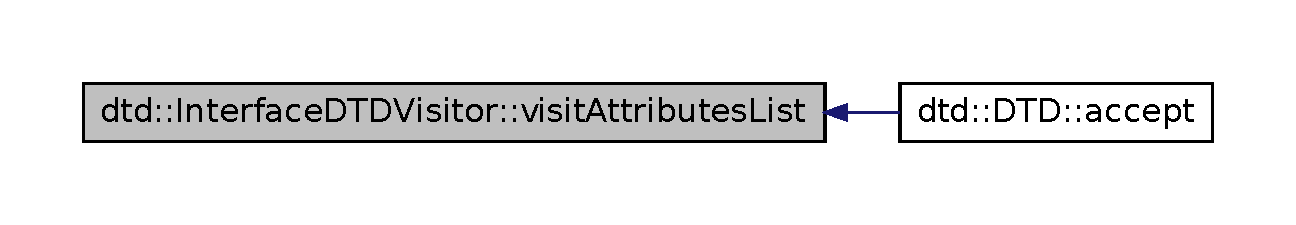
\includegraphics[width=400pt]{classdtd_1_1_interface_d_t_d_visitor_a729d9fcb360d9bf45210aac109b388da_icgraph}
\end{center}
\end{figure}


\hypertarget{classdtd_1_1_interface_d_t_d_visitor_a46b882a06961ea04fd43b2a9d937118b}{
\index{dtd::InterfaceDTDVisitor@{dtd::InterfaceDTDVisitor}!visitElement@{visitElement}}
\index{visitElement@{visitElement}!dtd::InterfaceDTDVisitor@{dtd::InterfaceDTDVisitor}}
\subsubsection[{visitElement}]{\setlength{\rightskip}{0pt plus 5cm}virtual void dtd::InterfaceDTDVisitor::visitElement (
\begin{DoxyParamCaption}
\item[{const std::string \&}]{ ns, }
\item[{const std::string \&}]{ elementName, }
\item[{const {\bf Content} \&}]{ content}
\end{DoxyParamCaption}
)\hspace{0.3cm}{\ttfamily  \mbox{[}pure virtual\mbox{]}}}}
\label{classdtd_1_1_interface_d_t_d_visitor_a46b882a06961ea04fd43b2a9d937118b}


Implémenté dans \hyperlink{classdtd_1_1_output_d_t_d_visitor_ab95fcc93547eb5e038040f11b0f2b568}{dtd::OutputDTDVisitor}.



Voici le graphe d'appel pour cette fonction :\nopagebreak
\begin{figure}[H]
\begin{center}
\leavevmode
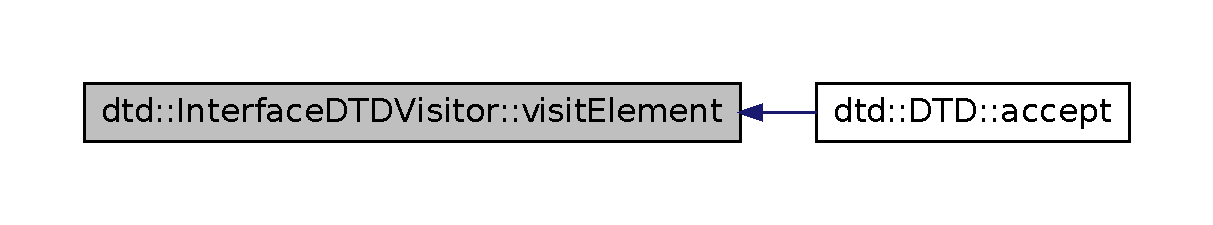
\includegraphics[width=400pt]{classdtd_1_1_interface_d_t_d_visitor_a46b882a06961ea04fd43b2a9d937118b_icgraph}
\end{center}
\end{figure}




\subsection{Documentation des fonctions amies et associées}
\hypertarget{classdtd_1_1_interface_d_t_d_visitor_a98eaefc8d4a0da1a8f9c254c62a68759}{
\index{dtd::InterfaceDTDVisitor@{dtd::InterfaceDTDVisitor}!AnyContent@{AnyContent}}
\index{AnyContent@{AnyContent}!dtd::InterfaceDTDVisitor@{dtd::InterfaceDTDVisitor}}
\subsubsection[{AnyContent}]{\setlength{\rightskip}{0pt plus 5cm}friend class {\bf AnyContent}\hspace{0.3cm}{\ttfamily  \mbox{[}friend\mbox{]}}}}
\label{classdtd_1_1_interface_d_t_d_visitor_a98eaefc8d4a0da1a8f9c254c62a68759}


Définition à la ligne 56 du fichier InterfaceDTDVisitor.hpp.

\hypertarget{classdtd_1_1_interface_d_t_d_visitor_af8084f88f5641132057732496deab026}{
\index{dtd::InterfaceDTDVisitor@{dtd::InterfaceDTDVisitor}!Choice@{Choice}}
\index{Choice@{Choice}!dtd::InterfaceDTDVisitor@{dtd::InterfaceDTDVisitor}}
\subsubsection[{Choice}]{\setlength{\rightskip}{0pt plus 5cm}friend class {\bf Choice}\hspace{0.3cm}{\ttfamily  \mbox{[}friend\mbox{]}}}}
\label{classdtd_1_1_interface_d_t_d_visitor_af8084f88f5641132057732496deab026}


Définition à la ligne 61 du fichier InterfaceDTDVisitor.hpp.

\hypertarget{classdtd_1_1_interface_d_t_d_visitor_a21b7004458ebe5b88f6d6edb6d059a34}{
\index{dtd::InterfaceDTDVisitor@{dtd::InterfaceDTDVisitor}!ElementReference@{ElementReference}}
\index{ElementReference@{ElementReference}!dtd::InterfaceDTDVisitor@{dtd::InterfaceDTDVisitor}}
\subsubsection[{ElementReference}]{\setlength{\rightskip}{0pt plus 5cm}friend class {\bf ElementReference}\hspace{0.3cm}{\ttfamily  \mbox{[}friend\mbox{]}}}}
\label{classdtd_1_1_interface_d_t_d_visitor_a21b7004458ebe5b88f6d6edb6d059a34}


Définition à la ligne 60 du fichier InterfaceDTDVisitor.hpp.

\hypertarget{classdtd_1_1_interface_d_t_d_visitor_a91eaa900fb18be6cd9a7105c964666fb}{
\index{dtd::InterfaceDTDVisitor@{dtd::InterfaceDTDVisitor}!EmptyContent@{EmptyContent}}
\index{EmptyContent@{EmptyContent}!dtd::InterfaceDTDVisitor@{dtd::InterfaceDTDVisitor}}
\subsubsection[{EmptyContent}]{\setlength{\rightskip}{0pt plus 5cm}friend class {\bf EmptyContent}\hspace{0.3cm}{\ttfamily  \mbox{[}friend\mbox{]}}}}
\label{classdtd_1_1_interface_d_t_d_visitor_a91eaa900fb18be6cd9a7105c964666fb}


Définition à la ligne 57 du fichier InterfaceDTDVisitor.hpp.

\hypertarget{classdtd_1_1_interface_d_t_d_visitor_a94c4de9fad580ef7aa4f384bf0c2b861}{
\index{dtd::InterfaceDTDVisitor@{dtd::InterfaceDTDVisitor}!MixedContent@{MixedContent}}
\index{MixedContent@{MixedContent}!dtd::InterfaceDTDVisitor@{dtd::InterfaceDTDVisitor}}
\subsubsection[{MixedContent}]{\setlength{\rightskip}{0pt plus 5cm}friend class {\bf MixedContent}\hspace{0.3cm}{\ttfamily  \mbox{[}friend\mbox{]}}}}
\label{classdtd_1_1_interface_d_t_d_visitor_a94c4de9fad580ef7aa4f384bf0c2b861}


Définition à la ligne 58 du fichier InterfaceDTDVisitor.hpp.

\hypertarget{classdtd_1_1_interface_d_t_d_visitor_a90839fb65068433fb68ba4e59462f869}{
\index{dtd::InterfaceDTDVisitor@{dtd::InterfaceDTDVisitor}!OptionalContent@{OptionalContent}}
\index{OptionalContent@{OptionalContent}!dtd::InterfaceDTDVisitor@{dtd::InterfaceDTDVisitor}}
\subsubsection[{OptionalContent}]{\setlength{\rightskip}{0pt plus 5cm}friend class {\bf OptionalContent}\hspace{0.3cm}{\ttfamily  \mbox{[}friend\mbox{]}}}}
\label{classdtd_1_1_interface_d_t_d_visitor_a90839fb65068433fb68ba4e59462f869}


Définition à la ligne 63 du fichier InterfaceDTDVisitor.hpp.

\hypertarget{classdtd_1_1_interface_d_t_d_visitor_ad2e096c883291671a8d20ca270018e05}{
\index{dtd::InterfaceDTDVisitor@{dtd::InterfaceDTDVisitor}!RepeatableContent@{RepeatableContent}}
\index{RepeatableContent@{RepeatableContent}!dtd::InterfaceDTDVisitor@{dtd::InterfaceDTDVisitor}}
\subsubsection[{RepeatableContent}]{\setlength{\rightskip}{0pt plus 5cm}friend class {\bf RepeatableContent}\hspace{0.3cm}{\ttfamily  \mbox{[}friend\mbox{]}}}}
\label{classdtd_1_1_interface_d_t_d_visitor_ad2e096c883291671a8d20ca270018e05}


Définition à la ligne 64 du fichier InterfaceDTDVisitor.hpp.

\hypertarget{classdtd_1_1_interface_d_t_d_visitor_afaa2f3eab18d4215d1683c4b2f5a6b8e}{
\index{dtd::InterfaceDTDVisitor@{dtd::InterfaceDTDVisitor}!RepeatedContent@{RepeatedContent}}
\index{RepeatedContent@{RepeatedContent}!dtd::InterfaceDTDVisitor@{dtd::InterfaceDTDVisitor}}
\subsubsection[{RepeatedContent}]{\setlength{\rightskip}{0pt plus 5cm}friend class {\bf RepeatedContent}\hspace{0.3cm}{\ttfamily  \mbox{[}friend\mbox{]}}}}
\label{classdtd_1_1_interface_d_t_d_visitor_afaa2f3eab18d4215d1683c4b2f5a6b8e}


Définition à la ligne 65 du fichier InterfaceDTDVisitor.hpp.

\hypertarget{classdtd_1_1_interface_d_t_d_visitor_a26271d5afaff6e6d3f00c055c63d0b24}{
\index{dtd::InterfaceDTDVisitor@{dtd::InterfaceDTDVisitor}!Sequence@{Sequence}}
\index{Sequence@{Sequence}!dtd::InterfaceDTDVisitor@{dtd::InterfaceDTDVisitor}}
\subsubsection[{Sequence}]{\setlength{\rightskip}{0pt plus 5cm}friend class {\bf Sequence}\hspace{0.3cm}{\ttfamily  \mbox{[}friend\mbox{]}}}}
\label{classdtd_1_1_interface_d_t_d_visitor_a26271d5afaff6e6d3f00c055c63d0b24}


Définition à la ligne 62 du fichier InterfaceDTDVisitor.hpp.

\hypertarget{classdtd_1_1_interface_d_t_d_visitor_aa641efa971cba38c6181cdc71b30df90}{
\index{dtd::InterfaceDTDVisitor@{dtd::InterfaceDTDVisitor}!TextContent@{TextContent}}
\index{TextContent@{TextContent}!dtd::InterfaceDTDVisitor@{dtd::InterfaceDTDVisitor}}
\subsubsection[{TextContent}]{\setlength{\rightskip}{0pt plus 5cm}friend class {\bf TextContent}\hspace{0.3cm}{\ttfamily  \mbox{[}friend\mbox{]}}}}
\label{classdtd_1_1_interface_d_t_d_visitor_aa641efa971cba38c6181cdc71b30df90}


Définition à la ligne 59 du fichier InterfaceDTDVisitor.hpp.



La documentation de cette classe a été générée à partir du fichier suivant :\begin{DoxyCompactItemize}
\item 
src/\hyperlink{_interface_d_t_d_visitor_8hpp}{InterfaceDTDVisitor.hpp}\end{DoxyCompactItemize}

\hypertarget{classdtd_1_1_mixed_content}{
\section{Référence de la classe dtd::MixedContent}
\label{classdtd_1_1_mixed_content}\index{dtd::MixedContent@{dtd::MixedContent}}
}


{\ttfamily \#include $<$MixedContent.hh$>$}



Graphe d'héritage de dtd::MixedContent:\nopagebreak
\begin{figure}[H]
\begin{center}
\leavevmode
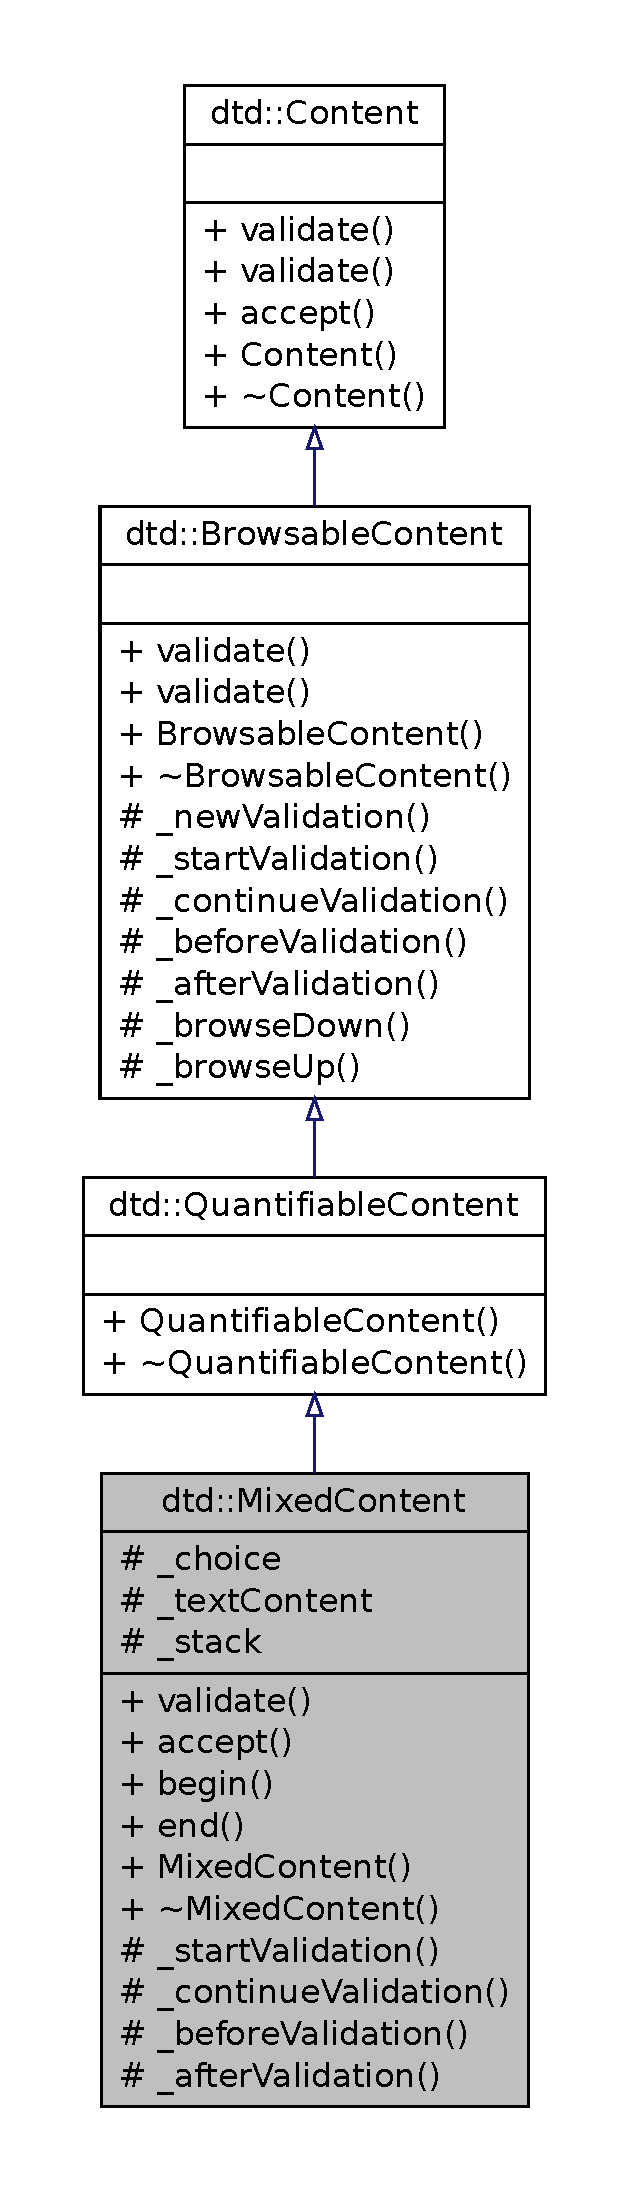
\includegraphics[height=600pt]{classdtd_1_1_mixed_content__inherit__graph}
\end{center}
\end{figure}


Graphe de collaboration de dtd::MixedContent:\nopagebreak
\begin{figure}[H]
\begin{center}
\leavevmode
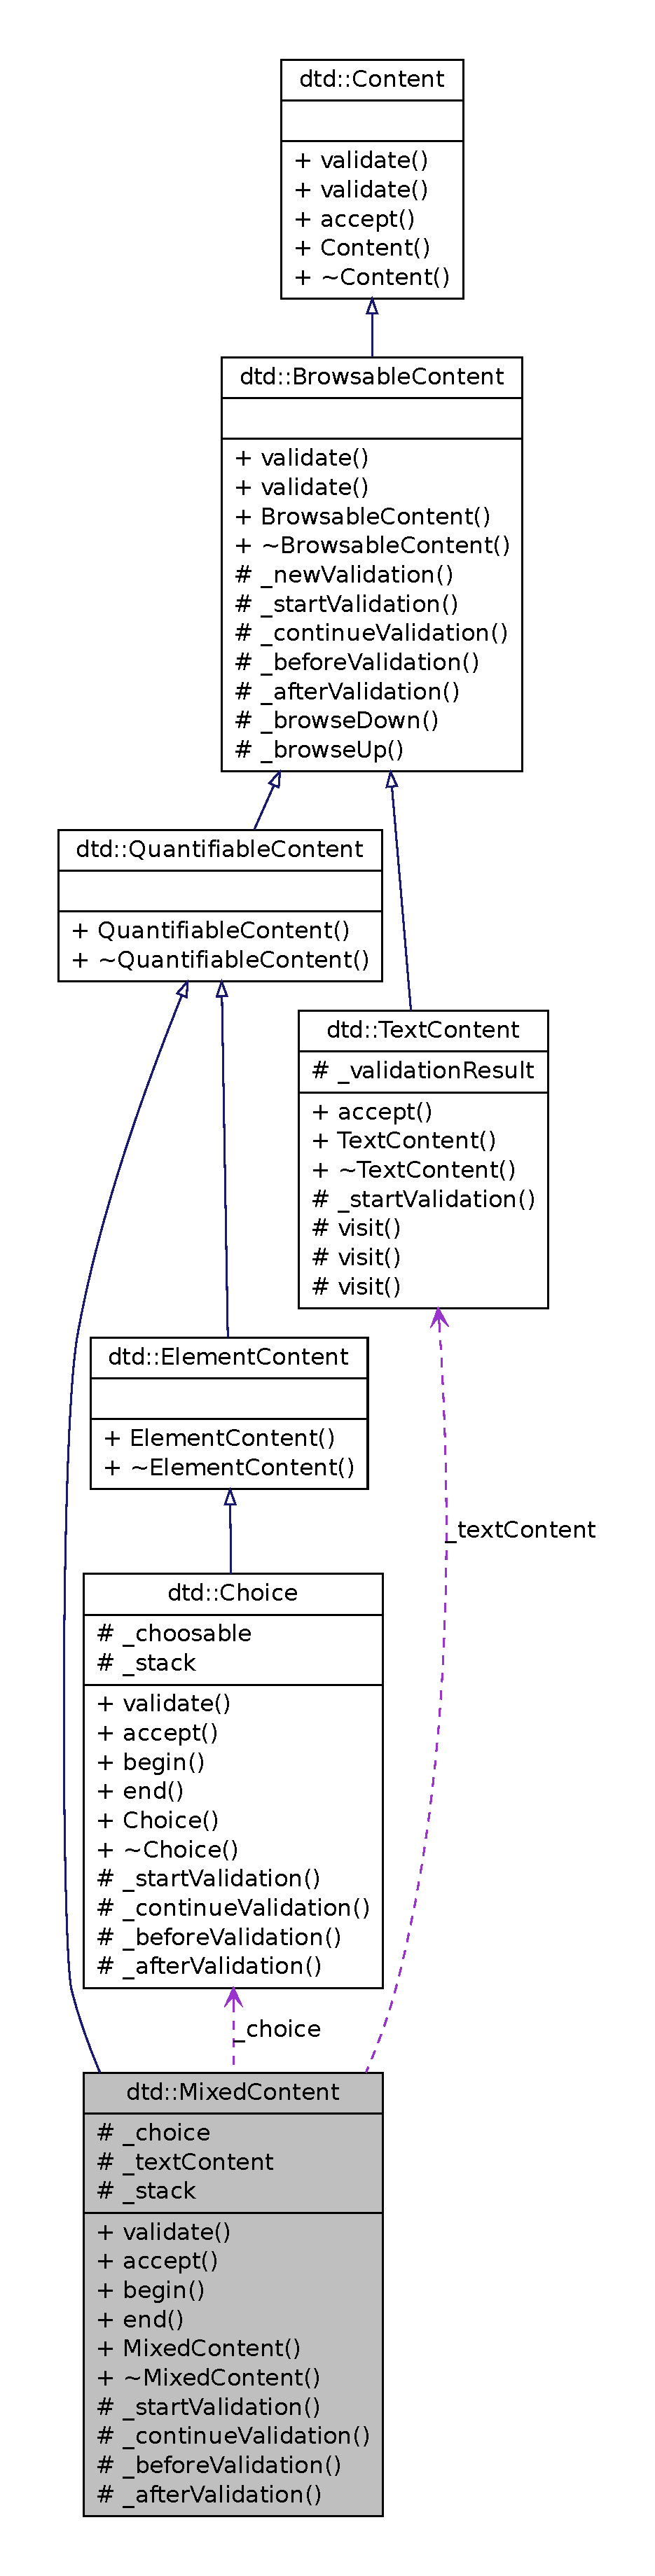
\includegraphics[height=600pt]{classdtd_1_1_mixed_content__coll__graph}
\end{center}
\end{figure}
\subsection*{Types publics}
\begin{DoxyCompactItemize}
\item 
typedef \hyperlink{classdtd_1_1_choice_af9629ca325eb99da3f274b2ad3dc2060}{Choice::ChoosableSet} \hyperlink{classdtd_1_1_mixed_content_ab8f0c26935279ce90ebb5bb22b244088}{ChoosableSet}
\item 
typedef ChoosableSet::const\_\-iterator \hyperlink{classdtd_1_1_mixed_content_a801684f467b642e9e2de6297585ccf7b}{const\_\-iterator}
\end{DoxyCompactItemize}
\subsection*{Fonctions membres publiques}
\begin{DoxyCompactItemize}
\item 
virtual bool \hyperlink{classdtd_1_1_mixed_content_a675bca1039d5dd8cced7fddb856428fd}{validate} (const xml::CompositeMarkupNode \&node)
\item 
virtual void \hyperlink{classdtd_1_1_mixed_content_aea7a1312dc631047db037c84899f7a05}{accept} (\hyperlink{classdtd_1_1_interface_d_t_d_visitor}{InterfaceDTDVisitor} \&visitor) const 
\item 
\hyperlink{classdtd_1_1_mixed_content_a801684f467b642e9e2de6297585ccf7b}{const\_\-iterator} \hyperlink{classdtd_1_1_mixed_content_ae329052b86f20252a7adeab321b35379}{begin} () const 
\item 
\hyperlink{classdtd_1_1_mixed_content_a801684f467b642e9e2de6297585ccf7b}{const\_\-iterator} \hyperlink{classdtd_1_1_mixed_content_a1d33a3179772862e611c962b23b7ff38}{end} () const 
\item 
\hyperlink{classdtd_1_1_mixed_content_ab853de43d13c98055cce02fa0175e3b2}{MixedContent} (\hyperlink{classdtd_1_1_text_content}{TextContent} \&textContent, const \hyperlink{classdtd_1_1_mixed_content_ab8f0c26935279ce90ebb5bb22b244088}{ChoosableSet} \&choosable)
\item 
virtual \hyperlink{classdtd_1_1_mixed_content_acadef0055c07eeecb917f503d9824df7}{$\sim$MixedContent} ()
\end{DoxyCompactItemize}
\subsection*{Types protégés}
\begin{DoxyCompactItemize}
\item 
typedef std::stack$<$ \hyperlink{structdtd_1_1_quantifiable_content_1_1___state}{\_\-State} $>$ \hyperlink{classdtd_1_1_mixed_content_af406cf95bf434a84082758aab801296d}{\_\-StatesStack}
\end{DoxyCompactItemize}
\subsection*{Fonctions membres protégées}
\begin{DoxyCompactItemize}
\item 
virtual bool \hyperlink{classdtd_1_1_mixed_content_ae2b12465df5873a58676315a563d1581}{\_\-startValidation} (xml::CompositeMarkupNode::ChildrenIterator firstToken, xml::CompositeMarkupNode::ChildrenIterator endToken, \hyperlink{classdtd_1_1_browsable_content}{BrowsableContent} $\ast$nextStep)
\item 
virtual bool \hyperlink{classdtd_1_1_mixed_content_a20d254e2b4366855818e1dd033d0736d}{\_\-continueValidation} (xml::CompositeMarkupNode::ChildrenIterator currentToken)
\item 
virtual void \hyperlink{classdtd_1_1_mixed_content_abb31ae73269d3bb10e6f5379332b1459}{\_\-beforeValidation} (xml::CompositeMarkupNode::ChildrenIterator firstToken, xml::CompositeMarkupNode::ChildrenIterator endToken, \hyperlink{classdtd_1_1_browsable_content}{BrowsableContent} $\ast$nextStep)
\item 
virtual void \hyperlink{classdtd_1_1_mixed_content_a1ad4f7436239c9cc9bd792b85447ee6b}{\_\-afterValidation} ()
\end{DoxyCompactItemize}
\subsection*{Attributs protégés}
\begin{DoxyCompactItemize}
\item 
\hyperlink{classdtd_1_1_choice}{Choice} \hyperlink{classdtd_1_1_mixed_content_a69bcdfa733df68aee3d6d48b8ee9fab1}{\_\-choice}
\item 
\hyperlink{classdtd_1_1_text_content}{TextContent} \& \hyperlink{classdtd_1_1_mixed_content_af8e3d219de7501a3cd397e913be22f2f}{\_\-textContent}
\item 
\hyperlink{classdtd_1_1_mixed_content_af406cf95bf434a84082758aab801296d}{\_\-StatesStack} \hyperlink{classdtd_1_1_mixed_content_a8da3d196eb875933a34c03190e1b3702}{\_\-stack}
\end{DoxyCompactItemize}


\subsection{Description détaillée}


Définition à la ligne 21 du fichier MixedContent.hh.



\subsection{Documentation des définitions de type membres}
\hypertarget{classdtd_1_1_mixed_content_af406cf95bf434a84082758aab801296d}{
\index{dtd::MixedContent@{dtd::MixedContent}!\_\-StatesStack@{\_\-StatesStack}}
\index{\_\-StatesStack@{\_\-StatesStack}!dtd::MixedContent@{dtd::MixedContent}}
\subsubsection[{\_\-StatesStack}]{\setlength{\rightskip}{0pt plus 5cm}typedef std::stack$<${\bf \_\-State}$>$ {\bf dtd::MixedContent::\_\-StatesStack}\hspace{0.3cm}{\ttfamily  \mbox{[}protected\mbox{]}}}}
\label{classdtd_1_1_mixed_content_af406cf95bf434a84082758aab801296d}


Définition à la ligne 84 du fichier MixedContent.hh.

\hypertarget{classdtd_1_1_mixed_content_ab8f0c26935279ce90ebb5bb22b244088}{
\index{dtd::MixedContent@{dtd::MixedContent}!ChoosableSet@{ChoosableSet}}
\index{ChoosableSet@{ChoosableSet}!dtd::MixedContent@{dtd::MixedContent}}
\subsubsection[{ChoosableSet}]{\setlength{\rightskip}{0pt plus 5cm}typedef {\bf Choice::ChoosableSet} {\bf dtd::MixedContent::ChoosableSet}}}
\label{classdtd_1_1_mixed_content_ab8f0c26935279ce90ebb5bb22b244088}


Définition à la ligne 29 du fichier MixedContent.hh.

\hypertarget{classdtd_1_1_mixed_content_a801684f467b642e9e2de6297585ccf7b}{
\index{dtd::MixedContent@{dtd::MixedContent}!const\_\-iterator@{const\_\-iterator}}
\index{const\_\-iterator@{const\_\-iterator}!dtd::MixedContent@{dtd::MixedContent}}
\subsubsection[{const\_\-iterator}]{\setlength{\rightskip}{0pt plus 5cm}typedef ChoosableSet::const\_\-iterator {\bf dtd::MixedContent::const\_\-iterator}}}
\label{classdtd_1_1_mixed_content_a801684f467b642e9e2de6297585ccf7b}


Définition à la ligne 30 du fichier MixedContent.hh.



\subsection{Documentation des constructeurs et destructeur}
\hypertarget{classdtd_1_1_mixed_content_ab853de43d13c98055cce02fa0175e3b2}{
\index{dtd::MixedContent@{dtd::MixedContent}!MixedContent@{MixedContent}}
\index{MixedContent@{MixedContent}!dtd::MixedContent@{dtd::MixedContent}}
\subsubsection[{MixedContent}]{\setlength{\rightskip}{0pt plus 5cm}dtd::MixedContent::MixedContent (
\begin{DoxyParamCaption}
\item[{{\bf TextContent} \&}]{ textContent, }
\item[{const {\bf ChoosableSet} \&}]{ choosable}
\end{DoxyParamCaption}
)}}
\label{classdtd_1_1_mixed_content_ab853de43d13c98055cce02fa0175e3b2}


Définition à la ligne 61 du fichier MixedContent.cpp.

\hypertarget{classdtd_1_1_mixed_content_acadef0055c07eeecb917f503d9824df7}{
\index{dtd::MixedContent@{dtd::MixedContent}!$\sim$MixedContent@{$\sim$MixedContent}}
\index{$\sim$MixedContent@{$\sim$MixedContent}!dtd::MixedContent@{dtd::MixedContent}}
\subsubsection[{$\sim$MixedContent}]{\setlength{\rightskip}{0pt plus 5cm}dtd::MixedContent::$\sim$MixedContent (
\begin{DoxyParamCaption}
{}
\end{DoxyParamCaption}
)\hspace{0.3cm}{\ttfamily  \mbox{[}virtual\mbox{]}}}}
\label{classdtd_1_1_mixed_content_acadef0055c07eeecb917f503d9824df7}


Définition à la ligne 68 du fichier MixedContent.cpp.



\subsection{Documentation des fonctions membres}
\hypertarget{classdtd_1_1_mixed_content_a1ad4f7436239c9cc9bd792b85447ee6b}{
\index{dtd::MixedContent@{dtd::MixedContent}!\_\-afterValidation@{\_\-afterValidation}}
\index{\_\-afterValidation@{\_\-afterValidation}!dtd::MixedContent@{dtd::MixedContent}}
\subsubsection[{\_\-afterValidation}]{\setlength{\rightskip}{0pt plus 5cm}void dtd::MixedContent::\_\-afterValidation (
\begin{DoxyParamCaption}
{}
\end{DoxyParamCaption}
)\hspace{0.3cm}{\ttfamily  \mbox{[}protected, virtual\mbox{]}}}}
\label{classdtd_1_1_mixed_content_a1ad4f7436239c9cc9bd792b85447ee6b}


Réimplémentée à partir de \hyperlink{classdtd_1_1_browsable_content_a378fc620af75eb9bad9f37c663e3838d}{dtd::BrowsableContent}.



Définition à la ligne 84 du fichier MixedContent.cpp.

\hypertarget{classdtd_1_1_mixed_content_abb31ae73269d3bb10e6f5379332b1459}{
\index{dtd::MixedContent@{dtd::MixedContent}!\_\-beforeValidation@{\_\-beforeValidation}}
\index{\_\-beforeValidation@{\_\-beforeValidation}!dtd::MixedContent@{dtd::MixedContent}}
\subsubsection[{\_\-beforeValidation}]{\setlength{\rightskip}{0pt plus 5cm}void dtd::MixedContent::\_\-beforeValidation (
\begin{DoxyParamCaption}
\item[{xml::CompositeMarkupNode::ChildrenIterator}]{ firstToken, }
\item[{xml::CompositeMarkupNode::ChildrenIterator}]{ endToken, }
\item[{{\bf BrowsableContent} $\ast$}]{ nextStep}
\end{DoxyParamCaption}
)\hspace{0.3cm}{\ttfamily  \mbox{[}protected, virtual\mbox{]}}}}
\label{classdtd_1_1_mixed_content_abb31ae73269d3bb10e6f5379332b1459}


Réimplémentée à partir de \hyperlink{classdtd_1_1_browsable_content_ae9e55da18cc09557fc7896a7ccac2ee1}{dtd::BrowsableContent}.



Définition à la ligne 76 du fichier MixedContent.cpp.

\hypertarget{classdtd_1_1_mixed_content_a20d254e2b4366855818e1dd033d0736d}{
\index{dtd::MixedContent@{dtd::MixedContent}!\_\-continueValidation@{\_\-continueValidation}}
\index{\_\-continueValidation@{\_\-continueValidation}!dtd::MixedContent@{dtd::MixedContent}}
\subsubsection[{\_\-continueValidation}]{\setlength{\rightskip}{0pt plus 5cm}bool dtd::MixedContent::\_\-continueValidation (
\begin{DoxyParamCaption}
\item[{xml::CompositeMarkupNode::ChildrenIterator}]{ currentToken}
\end{DoxyParamCaption}
)\hspace{0.3cm}{\ttfamily  \mbox{[}protected, virtual\mbox{]}}}}
\label{classdtd_1_1_mixed_content_a20d254e2b4366855818e1dd033d0736d}


Réimplémentée à partir de \hyperlink{classdtd_1_1_browsable_content_a6398e5990648e2af3fd775592b0d62ea}{dtd::BrowsableContent}.



Définition à la ligne 97 du fichier MixedContent.cpp.



Voici le graphe d'appel pour cette fonction :\nopagebreak
\begin{figure}[H]
\begin{center}
\leavevmode
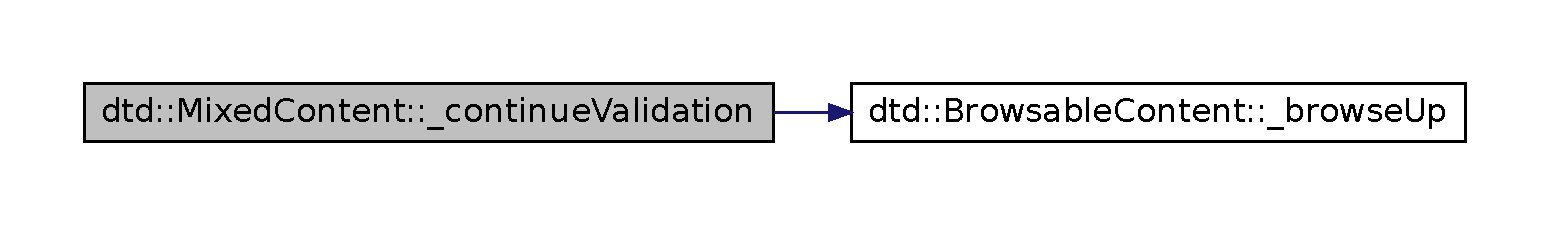
\includegraphics[width=400pt]{classdtd_1_1_mixed_content_a20d254e2b4366855818e1dd033d0736d_cgraph}
\end{center}
\end{figure}


\hypertarget{classdtd_1_1_mixed_content_ae2b12465df5873a58676315a563d1581}{
\index{dtd::MixedContent@{dtd::MixedContent}!\_\-startValidation@{\_\-startValidation}}
\index{\_\-startValidation@{\_\-startValidation}!dtd::MixedContent@{dtd::MixedContent}}
\subsubsection[{\_\-startValidation}]{\setlength{\rightskip}{0pt plus 5cm}virtual bool dtd::MixedContent::\_\-startValidation (
\begin{DoxyParamCaption}
\item[{xml::CompositeMarkupNode::ChildrenIterator}]{ firstToken, }
\item[{xml::CompositeMarkupNode::ChildrenIterator}]{ endToken, }
\item[{{\bf BrowsableContent} $\ast$}]{ nextStep}
\end{DoxyParamCaption}
)\hspace{0.3cm}{\ttfamily  \mbox{[}protected, virtual\mbox{]}}}}
\label{classdtd_1_1_mixed_content_ae2b12465df5873a58676315a563d1581}


Implémente \hyperlink{classdtd_1_1_browsable_content_a67ab5a7329d94e363796ae2d17617246}{dtd::BrowsableContent}.

\hypertarget{classdtd_1_1_mixed_content_aea7a1312dc631047db037c84899f7a05}{
\index{dtd::MixedContent@{dtd::MixedContent}!accept@{accept}}
\index{accept@{accept}!dtd::MixedContent@{dtd::MixedContent}}
\subsubsection[{accept}]{\setlength{\rightskip}{0pt plus 5cm}void dtd::MixedContent::accept (
\begin{DoxyParamCaption}
\item[{{\bf InterfaceDTDVisitor} \&}]{ visitor}
\end{DoxyParamCaption}
) const\hspace{0.3cm}{\ttfamily  \mbox{[}virtual\mbox{]}}}}
\label{classdtd_1_1_mixed_content_aea7a1312dc631047db037c84899f7a05}


Implémente \hyperlink{classdtd_1_1_content_a403cc15f12eaa187ad493fa600540cd8}{dtd::Content}.



Définition à la ligne 42 du fichier MixedContent.cpp.



Voici le graphe d'appel pour cette fonction :\nopagebreak
\begin{figure}[H]
\begin{center}
\leavevmode
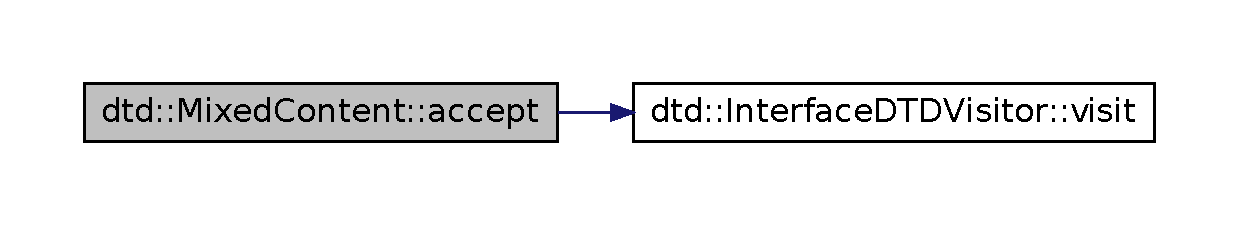
\includegraphics[width=400pt]{classdtd_1_1_mixed_content_aea7a1312dc631047db037c84899f7a05_cgraph}
\end{center}
\end{figure}


\hypertarget{classdtd_1_1_mixed_content_ae329052b86f20252a7adeab321b35379}{
\index{dtd::MixedContent@{dtd::MixedContent}!begin@{begin}}
\index{begin@{begin}!dtd::MixedContent@{dtd::MixedContent}}
\subsubsection[{begin}]{\setlength{\rightskip}{0pt plus 5cm}{\bf MixedContent::const\_\-iterator} dtd::MixedContent::begin (
\begin{DoxyParamCaption}
{}
\end{DoxyParamCaption}
) const}}
\label{classdtd_1_1_mixed_content_ae329052b86f20252a7adeab321b35379}


Définition à la ligne 47 du fichier MixedContent.cpp.

\hypertarget{classdtd_1_1_mixed_content_a1d33a3179772862e611c962b23b7ff38}{
\index{dtd::MixedContent@{dtd::MixedContent}!end@{end}}
\index{end@{end}!dtd::MixedContent@{dtd::MixedContent}}
\subsubsection[{end}]{\setlength{\rightskip}{0pt plus 5cm}{\bf MixedContent::const\_\-iterator} dtd::MixedContent::end (
\begin{DoxyParamCaption}
{}
\end{DoxyParamCaption}
) const}}
\label{classdtd_1_1_mixed_content_a1d33a3179772862e611c962b23b7ff38}


Définition à la ligne 52 du fichier MixedContent.cpp.

\hypertarget{classdtd_1_1_mixed_content_a675bca1039d5dd8cced7fddb856428fd}{
\index{dtd::MixedContent@{dtd::MixedContent}!validate@{validate}}
\index{validate@{validate}!dtd::MixedContent@{dtd::MixedContent}}
\subsubsection[{validate}]{\setlength{\rightskip}{0pt plus 5cm}virtual bool dtd::MixedContent::validate (
\begin{DoxyParamCaption}
\item[{const xml::CompositeMarkupNode \&}]{ node}
\end{DoxyParamCaption}
)\hspace{0.3cm}{\ttfamily  \mbox{[}virtual\mbox{]}}}}
\label{classdtd_1_1_mixed_content_a675bca1039d5dd8cced7fddb856428fd}


Réimplémentée à partir de \hyperlink{classdtd_1_1_browsable_content_a824a0c41b66aeea689e4283ee453d398}{dtd::BrowsableContent}.



\subsection{Documentation des données membres}
\hypertarget{classdtd_1_1_mixed_content_a69bcdfa733df68aee3d6d48b8ee9fab1}{
\index{dtd::MixedContent@{dtd::MixedContent}!\_\-choice@{\_\-choice}}
\index{\_\-choice@{\_\-choice}!dtd::MixedContent@{dtd::MixedContent}}
\subsubsection[{\_\-choice}]{\setlength{\rightskip}{0pt plus 5cm}{\bf Choice} {\bf dtd::MixedContent::\_\-choice}\hspace{0.3cm}{\ttfamily  \mbox{[}protected\mbox{]}}}}
\label{classdtd_1_1_mixed_content_a69bcdfa733df68aee3d6d48b8ee9fab1}


Définition à la ligne 81 du fichier MixedContent.hh.

\hypertarget{classdtd_1_1_mixed_content_a8da3d196eb875933a34c03190e1b3702}{
\index{dtd::MixedContent@{dtd::MixedContent}!\_\-stack@{\_\-stack}}
\index{\_\-stack@{\_\-stack}!dtd::MixedContent@{dtd::MixedContent}}
\subsubsection[{\_\-stack}]{\setlength{\rightskip}{0pt plus 5cm}{\bf \_\-StatesStack} {\bf dtd::MixedContent::\_\-stack}\hspace{0.3cm}{\ttfamily  \mbox{[}protected\mbox{]}}}}
\label{classdtd_1_1_mixed_content_a8da3d196eb875933a34c03190e1b3702}


Définition à la ligne 85 du fichier MixedContent.hh.

\hypertarget{classdtd_1_1_mixed_content_af8e3d219de7501a3cd397e913be22f2f}{
\index{dtd::MixedContent@{dtd::MixedContent}!\_\-textContent@{\_\-textContent}}
\index{\_\-textContent@{\_\-textContent}!dtd::MixedContent@{dtd::MixedContent}}
\subsubsection[{\_\-textContent}]{\setlength{\rightskip}{0pt plus 5cm}{\bf TextContent}\& {\bf dtd::MixedContent::\_\-textContent}\hspace{0.3cm}{\ttfamily  \mbox{[}protected\mbox{]}}}}
\label{classdtd_1_1_mixed_content_af8e3d219de7501a3cd397e913be22f2f}


Définition à la ligne 82 du fichier MixedContent.hh.



La documentation de cette classe a été générée à partir des fichiers suivants :\begin{DoxyCompactItemize}
\item 
src/\hyperlink{_mixed_content_8hh}{MixedContent.hh}\item 
src/\hyperlink{_mixed_content_8cpp}{MixedContent.cpp}\end{DoxyCompactItemize}

\hypertarget{classdtd_1_1_optional_content}{
\section{Référence de la classe dtd::OptionalContent}
\label{classdtd_1_1_optional_content}\index{dtd::OptionalContent@{dtd::OptionalContent}}
}


{\ttfamily \#include $<$OptionalContent.hh$>$}



Graphe d'héritage de dtd::OptionalContent:\nopagebreak
\begin{figure}[H]
\begin{center}
\leavevmode
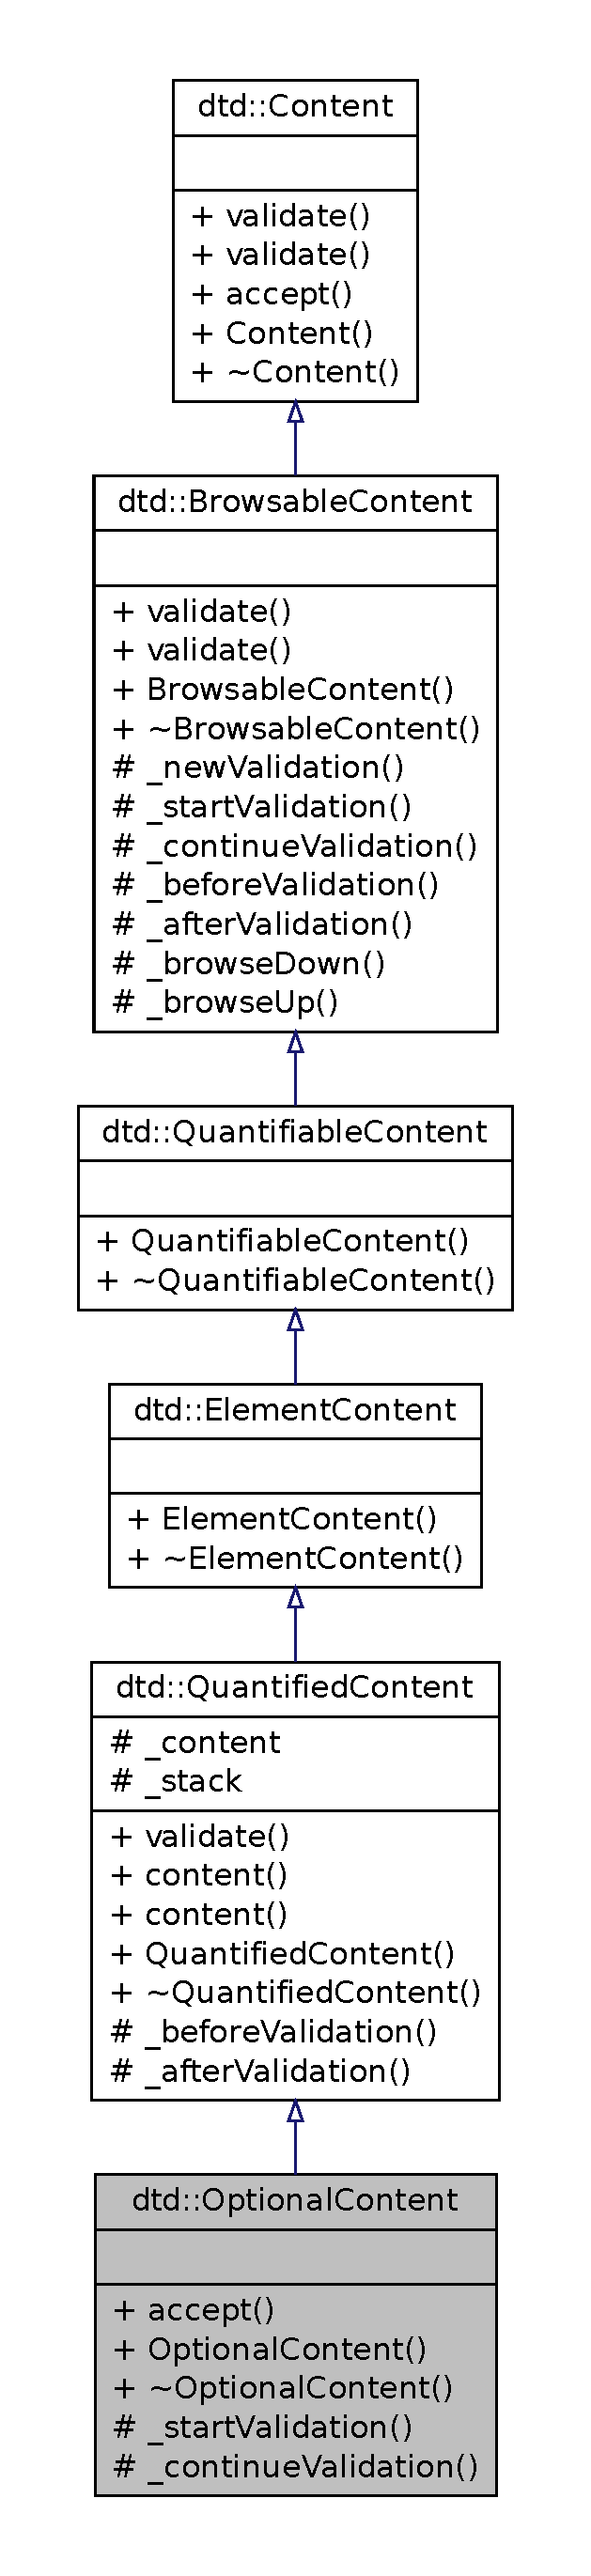
\includegraphics[height=600pt]{classdtd_1_1_optional_content__inherit__graph}
\end{center}
\end{figure}


Graphe de collaboration de dtd::OptionalContent:\nopagebreak
\begin{figure}[H]
\begin{center}
\leavevmode
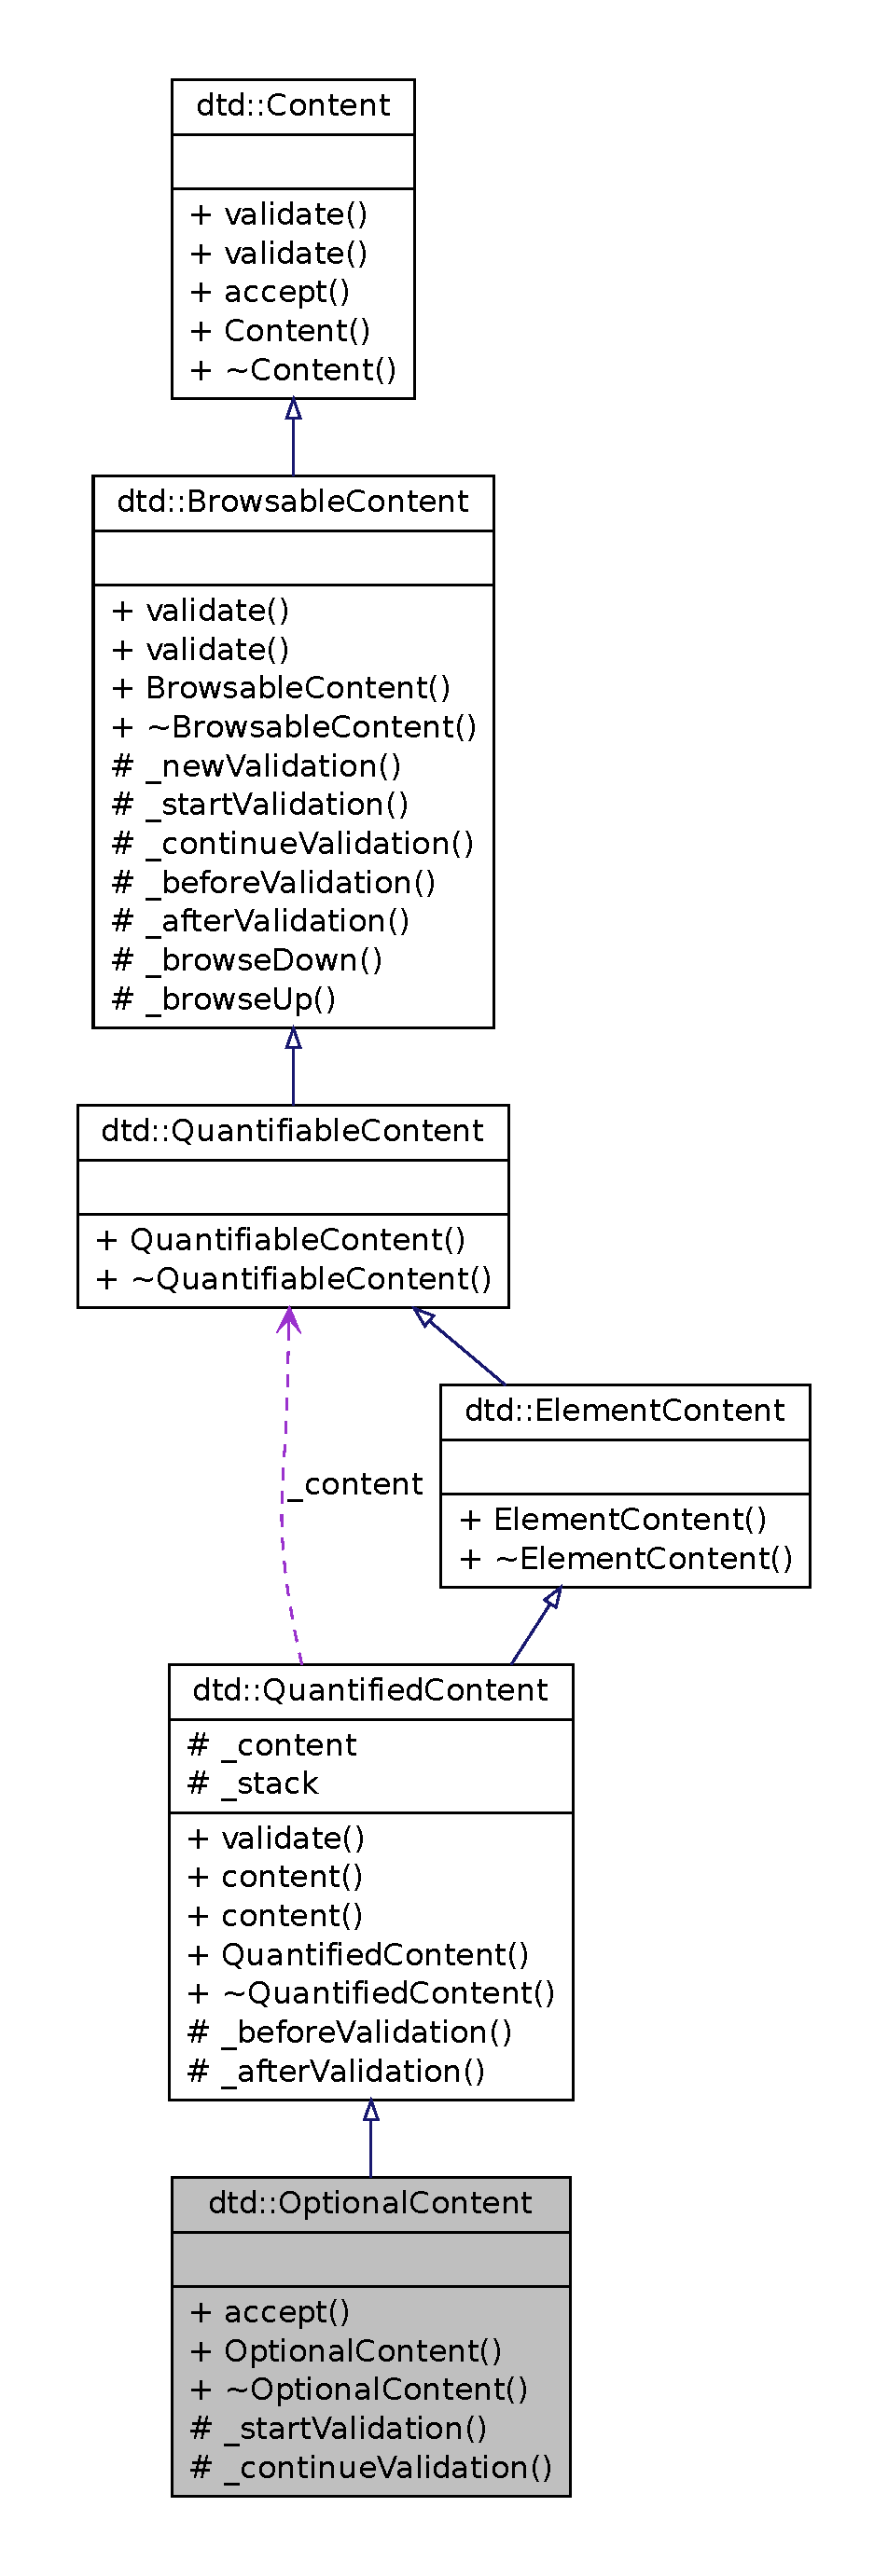
\includegraphics[height=600pt]{classdtd_1_1_optional_content__coll__graph}
\end{center}
\end{figure}
\subsection*{Fonctions membres publiques}
\begin{DoxyCompactItemize}
\item 
virtual void \hyperlink{classdtd_1_1_optional_content_a215be42249f1e54da514fdfc386ba21c}{accept} (\hyperlink{classdtd_1_1_interface_d_t_d_visitor}{InterfaceDTDVisitor} \&visitor) const 
\item 
\hyperlink{classdtd_1_1_optional_content_a93352de3e78f5279a80d19ae81ca7b71}{OptionalContent} (\hyperlink{classdtd_1_1_quantifiable_content}{QuantifiableContent} \&content)
\item 
virtual \hyperlink{classdtd_1_1_optional_content_aa10ed10083345b853a69319b79191e0d}{$\sim$OptionalContent} ()
\end{DoxyCompactItemize}
\subsection*{Fonctions membres protégées}
\begin{DoxyCompactItemize}
\item 
virtual bool \hyperlink{classdtd_1_1_optional_content_aeb537bd54c1c717d11fd1bd60f8f1b8f}{\_\-startValidation} (xml::CompositeMarkupNode::ChildrenIterator firstToken, xml::CompositeMarkupNode::ChildrenIterator endToken, \hyperlink{classdtd_1_1_browsable_content}{BrowsableContent} $\ast$nextStep)
\item 
virtual bool \hyperlink{classdtd_1_1_optional_content_ad299fdc7ddbac3df83c83cc93da8f6fe}{\_\-continueValidation} (xml::CompositeMarkupNode::ChildrenIterator currentToken)
\end{DoxyCompactItemize}


\subsection{Description détaillée}


Définition à la ligne 18 du fichier OptionalContent.hh.



\subsection{Documentation des constructeurs et destructeur}
\hypertarget{classdtd_1_1_optional_content_a93352de3e78f5279a80d19ae81ca7b71}{
\index{dtd::OptionalContent@{dtd::OptionalContent}!OptionalContent@{OptionalContent}}
\index{OptionalContent@{OptionalContent}!dtd::OptionalContent@{dtd::OptionalContent}}
\subsubsection[{OptionalContent}]{\setlength{\rightskip}{0pt plus 5cm}dtd::OptionalContent::OptionalContent (
\begin{DoxyParamCaption}
\item[{{\bf QuantifiableContent} \&}]{ content}
\end{DoxyParamCaption}
)}}
\label{classdtd_1_1_optional_content_a93352de3e78f5279a80d19ae81ca7b71}


Définition à la ligne 42 du fichier OptionalContent.cpp.

\hypertarget{classdtd_1_1_optional_content_aa10ed10083345b853a69319b79191e0d}{
\index{dtd::OptionalContent@{dtd::OptionalContent}!$\sim$OptionalContent@{$\sim$OptionalContent}}
\index{$\sim$OptionalContent@{$\sim$OptionalContent}!dtd::OptionalContent@{dtd::OptionalContent}}
\subsubsection[{$\sim$OptionalContent}]{\setlength{\rightskip}{0pt plus 5cm}dtd::OptionalContent::$\sim$OptionalContent (
\begin{DoxyParamCaption}
{}
\end{DoxyParamCaption}
)\hspace{0.3cm}{\ttfamily  \mbox{[}virtual\mbox{]}}}}
\label{classdtd_1_1_optional_content_aa10ed10083345b853a69319b79191e0d}


Définition à la ligne 48 du fichier OptionalContent.cpp.



\subsection{Documentation des fonctions membres}
\hypertarget{classdtd_1_1_optional_content_ad299fdc7ddbac3df83c83cc93da8f6fe}{
\index{dtd::OptionalContent@{dtd::OptionalContent}!\_\-continueValidation@{\_\-continueValidation}}
\index{\_\-continueValidation@{\_\-continueValidation}!dtd::OptionalContent@{dtd::OptionalContent}}
\subsubsection[{\_\-continueValidation}]{\setlength{\rightskip}{0pt plus 5cm}bool dtd::OptionalContent::\_\-continueValidation (
\begin{DoxyParamCaption}
\item[{xml::CompositeMarkupNode::ChildrenIterator}]{ currentToken}
\end{DoxyParamCaption}
)\hspace{0.3cm}{\ttfamily  \mbox{[}protected, virtual\mbox{]}}}}
\label{classdtd_1_1_optional_content_ad299fdc7ddbac3df83c83cc93da8f6fe}


Réimplémentée à partir de \hyperlink{classdtd_1_1_browsable_content_a6398e5990648e2af3fd775592b0d62ea}{dtd::BrowsableContent}.



Définition à la ligne 78 du fichier OptionalContent.cpp.



Voici le graphe d'appel pour cette fonction :\nopagebreak
\begin{figure}[H]
\begin{center}
\leavevmode
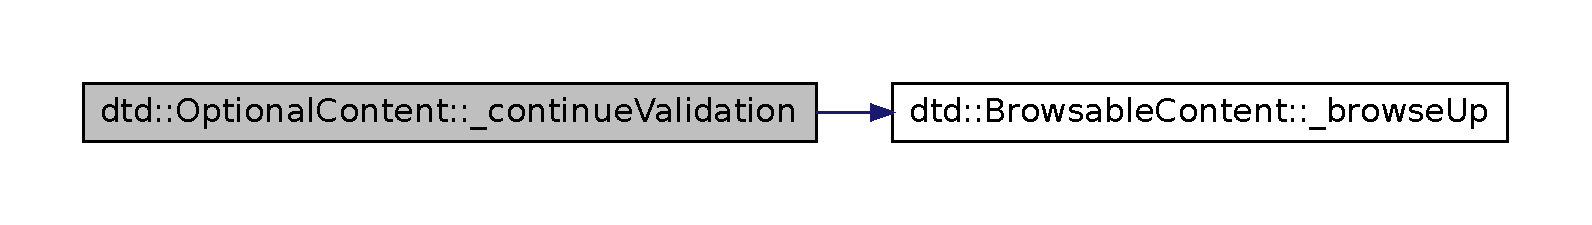
\includegraphics[width=400pt]{classdtd_1_1_optional_content_ad299fdc7ddbac3df83c83cc93da8f6fe_cgraph}
\end{center}
\end{figure}


\hypertarget{classdtd_1_1_optional_content_aeb537bd54c1c717d11fd1bd60f8f1b8f}{
\index{dtd::OptionalContent@{dtd::OptionalContent}!\_\-startValidation@{\_\-startValidation}}
\index{\_\-startValidation@{\_\-startValidation}!dtd::OptionalContent@{dtd::OptionalContent}}
\subsubsection[{\_\-startValidation}]{\setlength{\rightskip}{0pt plus 5cm}virtual bool dtd::OptionalContent::\_\-startValidation (
\begin{DoxyParamCaption}
\item[{xml::CompositeMarkupNode::ChildrenIterator}]{ firstToken, }
\item[{xml::CompositeMarkupNode::ChildrenIterator}]{ endToken, }
\item[{{\bf BrowsableContent} $\ast$}]{ nextStep}
\end{DoxyParamCaption}
)\hspace{0.3cm}{\ttfamily  \mbox{[}protected, virtual\mbox{]}}}}
\label{classdtd_1_1_optional_content_aeb537bd54c1c717d11fd1bd60f8f1b8f}


Implémente \hyperlink{classdtd_1_1_browsable_content_a67ab5a7329d94e363796ae2d17617246}{dtd::BrowsableContent}.

\hypertarget{classdtd_1_1_optional_content_a215be42249f1e54da514fdfc386ba21c}{
\index{dtd::OptionalContent@{dtd::OptionalContent}!accept@{accept}}
\index{accept@{accept}!dtd::OptionalContent@{dtd::OptionalContent}}
\subsubsection[{accept}]{\setlength{\rightskip}{0pt plus 5cm}void dtd::OptionalContent::accept (
\begin{DoxyParamCaption}
\item[{{\bf InterfaceDTDVisitor} \&}]{ visitor}
\end{DoxyParamCaption}
) const\hspace{0.3cm}{\ttfamily  \mbox{[}virtual\mbox{]}}}}
\label{classdtd_1_1_optional_content_a215be42249f1e54da514fdfc386ba21c}


Implémente \hyperlink{classdtd_1_1_content_a403cc15f12eaa187ad493fa600540cd8}{dtd::Content}.



Définition à la ligne 33 du fichier OptionalContent.cpp.



Voici le graphe d'appel pour cette fonction :\nopagebreak
\begin{figure}[H]
\begin{center}
\leavevmode
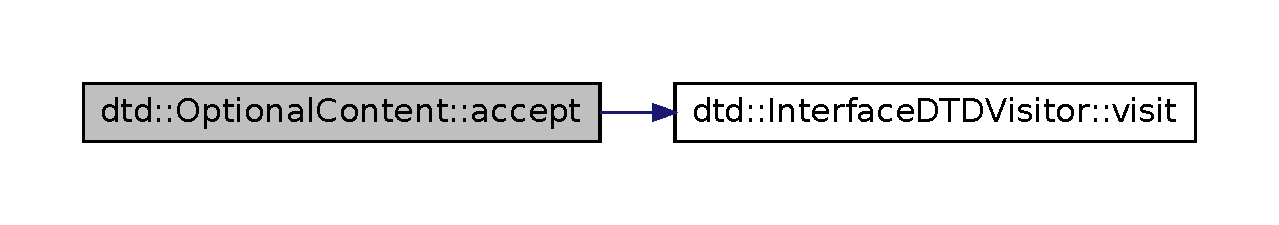
\includegraphics[width=400pt]{classdtd_1_1_optional_content_a215be42249f1e54da514fdfc386ba21c_cgraph}
\end{center}
\end{figure}




La documentation de cette classe a été générée à partir des fichiers suivants :\begin{DoxyCompactItemize}
\item 
src/\hyperlink{_optional_content_8hh}{OptionalContent.hh}\item 
src/\hyperlink{_optional_content_8cpp}{OptionalContent.cpp}\end{DoxyCompactItemize}

\hypertarget{classdtd_1_1_output_d_t_d_visitor}{
\section{Référence de la classe dtd::OutputDTDVisitor}
\label{classdtd_1_1_output_d_t_d_visitor}\index{dtd::OutputDTDVisitor@{dtd::OutputDTDVisitor}}
}


{\ttfamily \#include $<$OutputDTDVisitor.hh$>$}



Graphe d'héritage de dtd::OutputDTDVisitor:\nopagebreak
\begin{figure}[H]
\begin{center}
\leavevmode
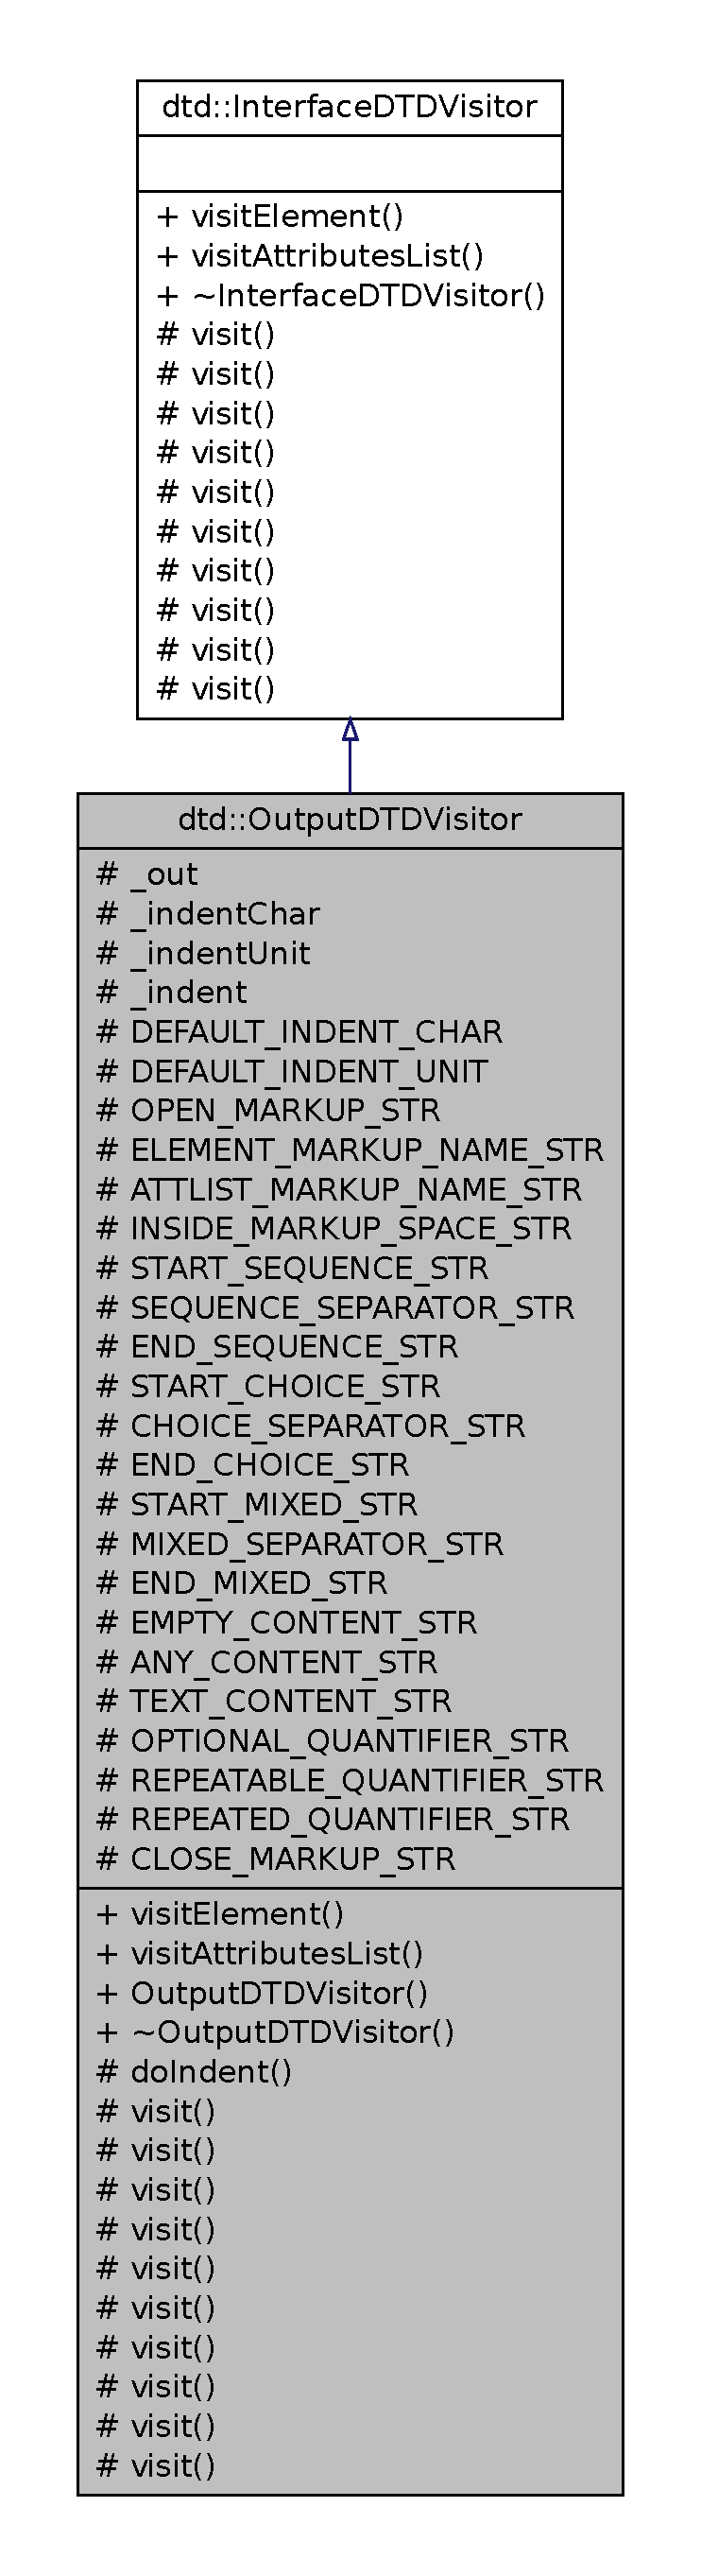
\includegraphics[height=600pt]{classdtd_1_1_output_d_t_d_visitor__inherit__graph}
\end{center}
\end{figure}


Graphe de collaboration de dtd::OutputDTDVisitor:\nopagebreak
\begin{figure}[H]
\begin{center}
\leavevmode
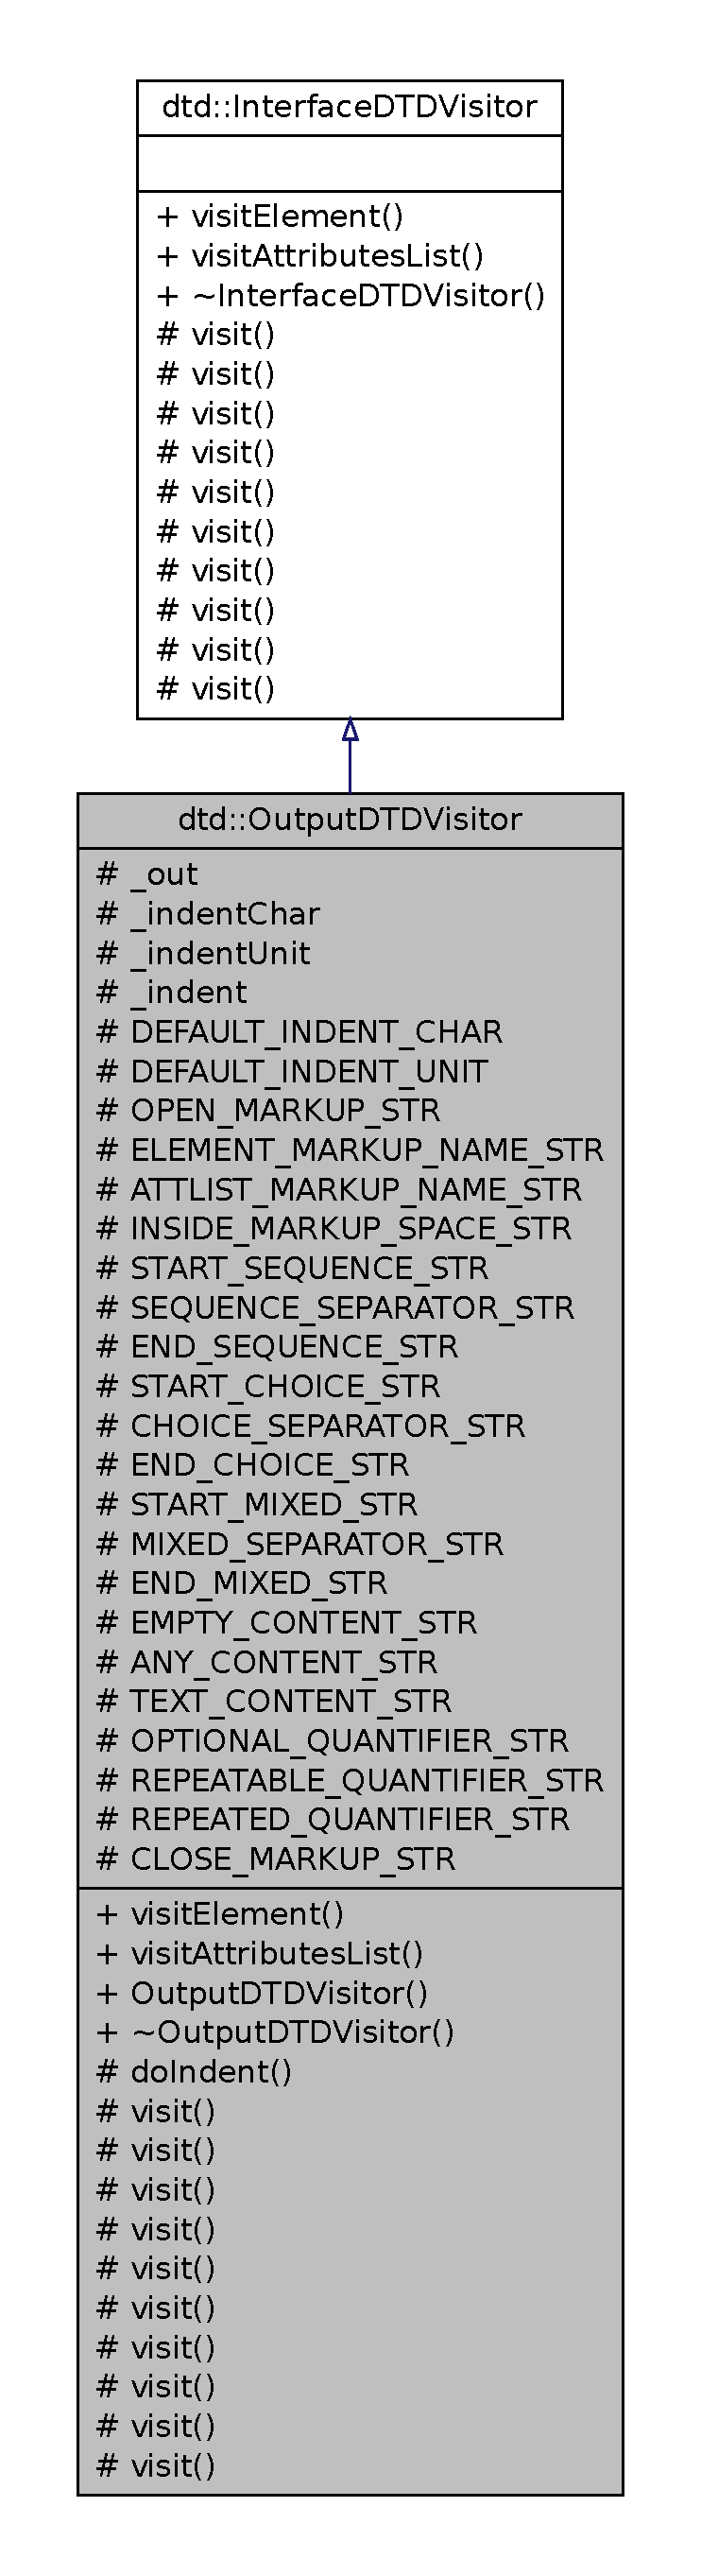
\includegraphics[height=600pt]{classdtd_1_1_output_d_t_d_visitor__coll__graph}
\end{center}
\end{figure}
\subsection*{Fonctions membres publiques}
\begin{DoxyCompactItemize}
\item 
virtual void \hyperlink{classdtd_1_1_output_d_t_d_visitor_ab95fcc93547eb5e038040f11b0f2b568}{visitElement} (const std::string \&ns, const std::string \&elementName, const \hyperlink{classdtd_1_1_content}{Content} \&content)
\item 
virtual void \hyperlink{classdtd_1_1_output_d_t_d_visitor_aa1b6474bd068eca43a6eb61e90ff7504}{visitAttributesList} (const std::string \&ns, const std::string \&elementName, const \hyperlink{namespacedtd_a8d5d29abb5de0468925f321597f57f4b}{AttributesList} \&attlist)
\item 
\hyperlink{classdtd_1_1_output_d_t_d_visitor_a08955c8d094f68867e38aff3d8dc43c8}{OutputDTDVisitor} (std::ostream \&out, char indentChar=\hyperlink{classdtd_1_1_output_d_t_d_visitor_af8b2c8e68ec262f98a21334900cb09df}{DEFAULT\_\-INDENT\_\-CHAR}, unsigned int indentUnit=\hyperlink{classdtd_1_1_output_d_t_d_visitor_a7795d56eeb6ab2e68c8d3a43e1c6f487}{DEFAULT\_\-INDENT\_\-UNIT})
\item 
virtual \hyperlink{classdtd_1_1_output_d_t_d_visitor_a718af27bc574809f02592f0816a71e2b}{$\sim$OutputDTDVisitor} ()
\end{DoxyCompactItemize}
\subsection*{Fonctions membres protégées}
\begin{DoxyCompactItemize}
\item 
void \hyperlink{classdtd_1_1_output_d_t_d_visitor_a5b8ee3a36a298245971b54b5307dd14f}{doIndent} ()
\item 
virtual void \hyperlink{classdtd_1_1_output_d_t_d_visitor_a3eb81ed67c53e9aebb90a4558f13a402}{visit} (const \hyperlink{classdtd_1_1_empty_content}{EmptyContent} \&content)
\item 
virtual void \hyperlink{classdtd_1_1_output_d_t_d_visitor_a17406ea51970e67da79947709945c4b1}{visit} (const \hyperlink{classdtd_1_1_any_content}{AnyContent} \&content)
\item 
virtual void \hyperlink{classdtd_1_1_output_d_t_d_visitor_a47692e383524d7804a6f5bf4d3f229b8}{visit} (const \hyperlink{classdtd_1_1_mixed_content}{MixedContent} \&content)
\item 
virtual void \hyperlink{classdtd_1_1_output_d_t_d_visitor_ad06e4a71ec8f36d91d59eb24ddc51f70}{visit} (const \hyperlink{classdtd_1_1_text_content}{TextContent} \&content)
\item 
virtual void \hyperlink{classdtd_1_1_output_d_t_d_visitor_a4b286b6b0ca83035e25cef1ba6f10c47}{visit} (const \hyperlink{classdtd_1_1_element_reference}{ElementReference} \&element)
\item 
virtual void \hyperlink{classdtd_1_1_output_d_t_d_visitor_a666c828c10840930fd420e86030e16f1}{visit} (const \hyperlink{classdtd_1_1_choice}{Choice} \&content)
\item 
virtual void \hyperlink{classdtd_1_1_output_d_t_d_visitor_a5b9434224d99c416da826a88cd11df3f}{visit} (const \hyperlink{classdtd_1_1_sequence}{Sequence} \&content)
\item 
virtual void \hyperlink{classdtd_1_1_output_d_t_d_visitor_a5ea91964e78eef4fc0786708154204bc}{visit} (const \hyperlink{classdtd_1_1_optional_content}{OptionalContent} \&content)
\item 
virtual void \hyperlink{classdtd_1_1_output_d_t_d_visitor_a93c6d6c010e58356bf9ba29b56d561df}{visit} (const \hyperlink{classdtd_1_1_repeatable_content}{RepeatableContent} \&content)
\item 
virtual void \hyperlink{classdtd_1_1_output_d_t_d_visitor_a01a2c44557480982c2ca5d3769e72c00}{visit} (const \hyperlink{classdtd_1_1_repeated_content}{RepeatedContent} \&content)
\end{DoxyCompactItemize}
\subsection*{Attributs protégés}
\begin{DoxyCompactItemize}
\item 
std::ostream \& \hyperlink{classdtd_1_1_output_d_t_d_visitor_a9a93007f2426887a2da46c30c5f2cc42}{\_\-out}
\item 
char \hyperlink{classdtd_1_1_output_d_t_d_visitor_ae58e26bcaaa7c8681209a13934cea5f7}{\_\-indentChar}
\item 
unsigned \hyperlink{classdtd_1_1_output_d_t_d_visitor_a913f11153a7fe38b61ff090d5bd99c89}{\_\-indentUnit}
\item 
unsigned int \hyperlink{classdtd_1_1_output_d_t_d_visitor_a8659c38013b7a5ba99e78c295a224362}{\_\-indent}
\end{DoxyCompactItemize}
\subsection*{Attributs protégés statiques}
\begin{DoxyCompactItemize}
\item 
static const char \hyperlink{classdtd_1_1_output_d_t_d_visitor_af8b2c8e68ec262f98a21334900cb09df}{DEFAULT\_\-INDENT\_\-CHAR} = '$\backslash$t'
\item 
static const unsigned char \hyperlink{classdtd_1_1_output_d_t_d_visitor_a7795d56eeb6ab2e68c8d3a43e1c6f487}{DEFAULT\_\-INDENT\_\-UNIT} = 1
\item 
static const std::string \hyperlink{classdtd_1_1_output_d_t_d_visitor_aac75a1ed1d3189d021a65c5d56d1527e}{OPEN\_\-MARKUP\_\-STR} = \char`\"{}$<$!\char`\"{}
\item 
static const std::string \hyperlink{classdtd_1_1_output_d_t_d_visitor_a14cd0eb333af784f38e3441c8fd1b97d}{ELEMENT\_\-MARKUP\_\-NAME\_\-STR} = \char`\"{}ELEMENT\char`\"{}
\item 
static const std::string \hyperlink{classdtd_1_1_output_d_t_d_visitor_a4ce2c50f68b4f167879b57e970ca662c}{ATTLIST\_\-MARKUP\_\-NAME\_\-STR} = \char`\"{}ATTLIST\char`\"{}
\item 
static const std::string \hyperlink{classdtd_1_1_output_d_t_d_visitor_a32ceb547a079fa2498ff14d1aef6e112}{INSIDE\_\-MARKUP\_\-SPACE\_\-STR} = \char`\"{} \char`\"{}
\item 
static const std::string \hyperlink{classdtd_1_1_output_d_t_d_visitor_a1b325fb88f176ce92e566fe4e6423c1c}{START\_\-SEQUENCE\_\-STR} = \char`\"{}(\char`\"{}
\item 
static const std::string \hyperlink{classdtd_1_1_output_d_t_d_visitor_acfffbc0db723271579d1fd87dc699b05}{SEQUENCE\_\-SEPARATOR\_\-STR} = \char`\"{},\char`\"{}
\item 
static const std::string \hyperlink{classdtd_1_1_output_d_t_d_visitor_a17ea023b24838b7b2a96fe56a2c574ea}{END\_\-SEQUENCE\_\-STR} = \char`\"{})\char`\"{}
\item 
static const std::string \hyperlink{classdtd_1_1_output_d_t_d_visitor_ae66777110076859a443e00a9da55ff1b}{START\_\-CHOICE\_\-STR} = \char`\"{}(\char`\"{}
\item 
static const std::string \hyperlink{classdtd_1_1_output_d_t_d_visitor_a686bb62aed37769865a688fe50e55f0a}{CHOICE\_\-SEPARATOR\_\-STR} = \char`\"{}$|$\char`\"{}
\item 
static const std::string \hyperlink{classdtd_1_1_output_d_t_d_visitor_ab0306525af8ca54d3279c02a2d79da46}{END\_\-CHOICE\_\-STR} = \char`\"{})\char`\"{}
\item 
static const std::string \hyperlink{classdtd_1_1_output_d_t_d_visitor_a254da51819583f6fd4501521f741042d}{START\_\-MIXED\_\-STR} = \char`\"{}(\char`\"{}
\item 
static const std::string \hyperlink{classdtd_1_1_output_d_t_d_visitor_af583c776fabca5615d43da966dca600c}{MIXED\_\-SEPARATOR\_\-STR} = \char`\"{}$|$\char`\"{}
\item 
static const std::string \hyperlink{classdtd_1_1_output_d_t_d_visitor_a217915df1bfe131dae99679461140fcc}{END\_\-MIXED\_\-STR} = \char`\"{})\char`\"{}
\item 
static const std::string \hyperlink{classdtd_1_1_output_d_t_d_visitor_af77ea7a3f4f05a3b3fea5a58a7d6de53}{EMPTY\_\-CONTENT\_\-STR} = \char`\"{}EMPTY\char`\"{}
\item 
static const std::string \hyperlink{classdtd_1_1_output_d_t_d_visitor_a4f8609bcd2c8c20d1de80081835c48fc}{ANY\_\-CONTENT\_\-STR} = \char`\"{}ANY\char`\"{}
\item 
static const std::string \hyperlink{classdtd_1_1_output_d_t_d_visitor_a83f802e6ceef88d9496b0aedf4d4541e}{TEXT\_\-CONTENT\_\-STR} = \char`\"{}\#PCDATA\char`\"{}
\item 
static const std::string \hyperlink{classdtd_1_1_output_d_t_d_visitor_a98f9105b5bccb426bc8a6e907a67b17f}{OPTIONAL\_\-QUANTIFIER\_\-STR} = \char`\"{}?\char`\"{}
\item 
static const std::string \hyperlink{classdtd_1_1_output_d_t_d_visitor_a4041af52751607ff7ae188484d962d95}{REPEATABLE\_\-QUANTIFIER\_\-STR} = \char`\"{}$\ast$\char`\"{}
\item 
static const std::string \hyperlink{classdtd_1_1_output_d_t_d_visitor_ae8c6ec6c1f6ae17d8705be7267b07a2f}{REPEATED\_\-QUANTIFIER\_\-STR} = \char`\"{}+\char`\"{}
\item 
static const std::string \hyperlink{classdtd_1_1_output_d_t_d_visitor_a4dbe0d3fda6b73977f28488cf2f9cff4}{CLOSE\_\-MARKUP\_\-STR} = \char`\"{}$>$\char`\"{}
\end{DoxyCompactItemize}


\subsection{Description détaillée}


Définition à la ligne 20 du fichier OutputDTDVisitor.hh.



\subsection{Documentation des constructeurs et destructeur}
\hypertarget{classdtd_1_1_output_d_t_d_visitor_a08955c8d094f68867e38aff3d8dc43c8}{
\index{dtd::OutputDTDVisitor@{dtd::OutputDTDVisitor}!OutputDTDVisitor@{OutputDTDVisitor}}
\index{OutputDTDVisitor@{OutputDTDVisitor}!dtd::OutputDTDVisitor@{dtd::OutputDTDVisitor}}
\subsubsection[{OutputDTDVisitor}]{\setlength{\rightskip}{0pt plus 5cm}dtd::OutputDTDVisitor::OutputDTDVisitor (
\begin{DoxyParamCaption}
\item[{std::ostream \&}]{ out, }
\item[{char}]{ indentChar = {\ttfamily {\bf DEFAULT\_\-INDENT\_\-CHAR}}, }
\item[{unsigned int}]{ indentUnit = {\ttfamily {\bf DEFAULT\_\-INDENT\_\-UNIT}}}
\end{DoxyParamCaption}
)}}
\label{classdtd_1_1_output_d_t_d_visitor_a08955c8d094f68867e38aff3d8dc43c8}


Définition à la ligne 94 du fichier OutputDTDVisitor.cpp.

\hypertarget{classdtd_1_1_output_d_t_d_visitor_a718af27bc574809f02592f0816a71e2b}{
\index{dtd::OutputDTDVisitor@{dtd::OutputDTDVisitor}!$\sim$OutputDTDVisitor@{$\sim$OutputDTDVisitor}}
\index{$\sim$OutputDTDVisitor@{$\sim$OutputDTDVisitor}!dtd::OutputDTDVisitor@{dtd::OutputDTDVisitor}}
\subsubsection[{$\sim$OutputDTDVisitor}]{\setlength{\rightskip}{0pt plus 5cm}dtd::OutputDTDVisitor::$\sim$OutputDTDVisitor (
\begin{DoxyParamCaption}
{}
\end{DoxyParamCaption}
)\hspace{0.3cm}{\ttfamily  \mbox{[}virtual\mbox{]}}}}
\label{classdtd_1_1_output_d_t_d_visitor_a718af27bc574809f02592f0816a71e2b}


Définition à la ligne 101 du fichier OutputDTDVisitor.cpp.



\subsection{Documentation des fonctions membres}
\hypertarget{classdtd_1_1_output_d_t_d_visitor_a5b8ee3a36a298245971b54b5307dd14f}{
\index{dtd::OutputDTDVisitor@{dtd::OutputDTDVisitor}!doIndent@{doIndent}}
\index{doIndent@{doIndent}!dtd::OutputDTDVisitor@{dtd::OutputDTDVisitor}}
\subsubsection[{doIndent}]{\setlength{\rightskip}{0pt plus 5cm}void dtd::OutputDTDVisitor::doIndent (
\begin{DoxyParamCaption}
{}
\end{DoxyParamCaption}
)\hspace{0.3cm}{\ttfamily  \mbox{[}protected\mbox{]}}}}
\label{classdtd_1_1_output_d_t_d_visitor_a5b8ee3a36a298245971b54b5307dd14f}


Définition à la ligne 110 du fichier OutputDTDVisitor.cpp.

\hypertarget{classdtd_1_1_output_d_t_d_visitor_a01a2c44557480982c2ca5d3769e72c00}{
\index{dtd::OutputDTDVisitor@{dtd::OutputDTDVisitor}!visit@{visit}}
\index{visit@{visit}!dtd::OutputDTDVisitor@{dtd::OutputDTDVisitor}}
\subsubsection[{visit}]{\setlength{\rightskip}{0pt plus 5cm}void dtd::OutputDTDVisitor::visit (
\begin{DoxyParamCaption}
\item[{const {\bf RepeatedContent} \&}]{ content}
\end{DoxyParamCaption}
)\hspace{0.3cm}{\ttfamily  \mbox{[}protected, virtual\mbox{]}}}}
\label{classdtd_1_1_output_d_t_d_visitor_a01a2c44557480982c2ca5d3769e72c00}


Implémente \hyperlink{classdtd_1_1_interface_d_t_d_visitor_a8a2ce739049697fcc2a7126adea4536a}{dtd::InterfaceDTDVisitor}.



Définition à la ligne 195 du fichier OutputDTDVisitor.cpp.

\hypertarget{classdtd_1_1_output_d_t_d_visitor_a3eb81ed67c53e9aebb90a4558f13a402}{
\index{dtd::OutputDTDVisitor@{dtd::OutputDTDVisitor}!visit@{visit}}
\index{visit@{visit}!dtd::OutputDTDVisitor@{dtd::OutputDTDVisitor}}
\subsubsection[{visit}]{\setlength{\rightskip}{0pt plus 5cm}void dtd::OutputDTDVisitor::visit (
\begin{DoxyParamCaption}
\item[{const {\bf EmptyContent} \&}]{ content}
\end{DoxyParamCaption}
)\hspace{0.3cm}{\ttfamily  \mbox{[}protected, virtual\mbox{]}}}}
\label{classdtd_1_1_output_d_t_d_visitor_a3eb81ed67c53e9aebb90a4558f13a402}


Implémente \hyperlink{classdtd_1_1_interface_d_t_d_visitor_abdf03eb698f07aa0caaa405711fc8aac}{dtd::InterfaceDTDVisitor}.



Définition à la ligne 125 du fichier OutputDTDVisitor.cpp.

\hypertarget{classdtd_1_1_output_d_t_d_visitor_a5ea91964e78eef4fc0786708154204bc}{
\index{dtd::OutputDTDVisitor@{dtd::OutputDTDVisitor}!visit@{visit}}
\index{visit@{visit}!dtd::OutputDTDVisitor@{dtd::OutputDTDVisitor}}
\subsubsection[{visit}]{\setlength{\rightskip}{0pt plus 5cm}void dtd::OutputDTDVisitor::visit (
\begin{DoxyParamCaption}
\item[{const {\bf OptionalContent} \&}]{ content}
\end{DoxyParamCaption}
)\hspace{0.3cm}{\ttfamily  \mbox{[}protected, virtual\mbox{]}}}}
\label{classdtd_1_1_output_d_t_d_visitor_a5ea91964e78eef4fc0786708154204bc}


Implémente \hyperlink{classdtd_1_1_interface_d_t_d_visitor_a444ada6db2f531579579de7b8fd5fd53}{dtd::InterfaceDTDVisitor}.



Définition à la ligne 183 du fichier OutputDTDVisitor.cpp.

\hypertarget{classdtd_1_1_output_d_t_d_visitor_a5b9434224d99c416da826a88cd11df3f}{
\index{dtd::OutputDTDVisitor@{dtd::OutputDTDVisitor}!visit@{visit}}
\index{visit@{visit}!dtd::OutputDTDVisitor@{dtd::OutputDTDVisitor}}
\subsubsection[{visit}]{\setlength{\rightskip}{0pt plus 5cm}void dtd::OutputDTDVisitor::visit (
\begin{DoxyParamCaption}
\item[{const {\bf Sequence} \&}]{ content}
\end{DoxyParamCaption}
)\hspace{0.3cm}{\ttfamily  \mbox{[}protected, virtual\mbox{]}}}}
\label{classdtd_1_1_output_d_t_d_visitor_a5b9434224d99c416da826a88cd11df3f}


Implémente \hyperlink{classdtd_1_1_interface_d_t_d_visitor_aa093199d020b5887fbaa8af1573afc51}{dtd::InterfaceDTDVisitor}.



Définition à la ligne 168 du fichier OutputDTDVisitor.cpp.

\hypertarget{classdtd_1_1_output_d_t_d_visitor_a4b286b6b0ca83035e25cef1ba6f10c47}{
\index{dtd::OutputDTDVisitor@{dtd::OutputDTDVisitor}!visit@{visit}}
\index{visit@{visit}!dtd::OutputDTDVisitor@{dtd::OutputDTDVisitor}}
\subsubsection[{visit}]{\setlength{\rightskip}{0pt plus 5cm}void dtd::OutputDTDVisitor::visit (
\begin{DoxyParamCaption}
\item[{const {\bf ElementReference} \&}]{ element}
\end{DoxyParamCaption}
)\hspace{0.3cm}{\ttfamily  \mbox{[}protected, virtual\mbox{]}}}}
\label{classdtd_1_1_output_d_t_d_visitor_a4b286b6b0ca83035e25cef1ba6f10c47}


Implémente \hyperlink{classdtd_1_1_interface_d_t_d_visitor_aaac54822c9519b08305a64aab110716b}{dtd::InterfaceDTDVisitor}.



Définition à la ligne 148 du fichier OutputDTDVisitor.cpp.

\hypertarget{classdtd_1_1_output_d_t_d_visitor_a666c828c10840930fd420e86030e16f1}{
\index{dtd::OutputDTDVisitor@{dtd::OutputDTDVisitor}!visit@{visit}}
\index{visit@{visit}!dtd::OutputDTDVisitor@{dtd::OutputDTDVisitor}}
\subsubsection[{visit}]{\setlength{\rightskip}{0pt plus 5cm}void dtd::OutputDTDVisitor::visit (
\begin{DoxyParamCaption}
\item[{const {\bf Choice} \&}]{ content}
\end{DoxyParamCaption}
)\hspace{0.3cm}{\ttfamily  \mbox{[}protected, virtual\mbox{]}}}}
\label{classdtd_1_1_output_d_t_d_visitor_a666c828c10840930fd420e86030e16f1}


Implémente \hyperlink{classdtd_1_1_interface_d_t_d_visitor_a4323aeef86fa385a44fd4572ccc36cd2}{dtd::InterfaceDTDVisitor}.



Définition à la ligne 153 du fichier OutputDTDVisitor.cpp.

\hypertarget{classdtd_1_1_output_d_t_d_visitor_ad06e4a71ec8f36d91d59eb24ddc51f70}{
\index{dtd::OutputDTDVisitor@{dtd::OutputDTDVisitor}!visit@{visit}}
\index{visit@{visit}!dtd::OutputDTDVisitor@{dtd::OutputDTDVisitor}}
\subsubsection[{visit}]{\setlength{\rightskip}{0pt plus 5cm}void dtd::OutputDTDVisitor::visit (
\begin{DoxyParamCaption}
\item[{const {\bf TextContent} \&}]{ content}
\end{DoxyParamCaption}
)\hspace{0.3cm}{\ttfamily  \mbox{[}protected, virtual\mbox{]}}}}
\label{classdtd_1_1_output_d_t_d_visitor_ad06e4a71ec8f36d91d59eb24ddc51f70}


Implémente \hyperlink{classdtd_1_1_interface_d_t_d_visitor_abd31e761d6d8ab80ac6f3f0a9a20b953}{dtd::InterfaceDTDVisitor}.



Définition à la ligne 143 du fichier OutputDTDVisitor.cpp.

\hypertarget{classdtd_1_1_output_d_t_d_visitor_a93c6d6c010e58356bf9ba29b56d561df}{
\index{dtd::OutputDTDVisitor@{dtd::OutputDTDVisitor}!visit@{visit}}
\index{visit@{visit}!dtd::OutputDTDVisitor@{dtd::OutputDTDVisitor}}
\subsubsection[{visit}]{\setlength{\rightskip}{0pt plus 5cm}void dtd::OutputDTDVisitor::visit (
\begin{DoxyParamCaption}
\item[{const {\bf RepeatableContent} \&}]{ content}
\end{DoxyParamCaption}
)\hspace{0.3cm}{\ttfamily  \mbox{[}protected, virtual\mbox{]}}}}
\label{classdtd_1_1_output_d_t_d_visitor_a93c6d6c010e58356bf9ba29b56d561df}


Implémente \hyperlink{classdtd_1_1_interface_d_t_d_visitor_a76bd6fb0307eea7fc6ef703cf09a07b9}{dtd::InterfaceDTDVisitor}.



Définition à la ligne 189 du fichier OutputDTDVisitor.cpp.

\hypertarget{classdtd_1_1_output_d_t_d_visitor_a17406ea51970e67da79947709945c4b1}{
\index{dtd::OutputDTDVisitor@{dtd::OutputDTDVisitor}!visit@{visit}}
\index{visit@{visit}!dtd::OutputDTDVisitor@{dtd::OutputDTDVisitor}}
\subsubsection[{visit}]{\setlength{\rightskip}{0pt plus 5cm}void dtd::OutputDTDVisitor::visit (
\begin{DoxyParamCaption}
\item[{const {\bf AnyContent} \&}]{ content}
\end{DoxyParamCaption}
)\hspace{0.3cm}{\ttfamily  \mbox{[}protected, virtual\mbox{]}}}}
\label{classdtd_1_1_output_d_t_d_visitor_a17406ea51970e67da79947709945c4b1}


Implémente \hyperlink{classdtd_1_1_interface_d_t_d_visitor_ac2d1f472564e590bbe66f14ab096167a}{dtd::InterfaceDTDVisitor}.



Définition à la ligne 120 du fichier OutputDTDVisitor.cpp.

\hypertarget{classdtd_1_1_output_d_t_d_visitor_a47692e383524d7804a6f5bf4d3f229b8}{
\index{dtd::OutputDTDVisitor@{dtd::OutputDTDVisitor}!visit@{visit}}
\index{visit@{visit}!dtd::OutputDTDVisitor@{dtd::OutputDTDVisitor}}
\subsubsection[{visit}]{\setlength{\rightskip}{0pt plus 5cm}void dtd::OutputDTDVisitor::visit (
\begin{DoxyParamCaption}
\item[{const {\bf MixedContent} \&}]{ content}
\end{DoxyParamCaption}
)\hspace{0.3cm}{\ttfamily  \mbox{[}protected, virtual\mbox{]}}}}
\label{classdtd_1_1_output_d_t_d_visitor_a47692e383524d7804a6f5bf4d3f229b8}


Implémente \hyperlink{classdtd_1_1_interface_d_t_d_visitor_a06be244faf5995ac7ca502b326db10e0}{dtd::InterfaceDTDVisitor}.



Définition à la ligne 130 du fichier OutputDTDVisitor.cpp.

\hypertarget{classdtd_1_1_output_d_t_d_visitor_aa1b6474bd068eca43a6eb61e90ff7504}{
\index{dtd::OutputDTDVisitor@{dtd::OutputDTDVisitor}!visitAttributesList@{visitAttributesList}}
\index{visitAttributesList@{visitAttributesList}!dtd::OutputDTDVisitor@{dtd::OutputDTDVisitor}}
\subsubsection[{visitAttributesList}]{\setlength{\rightskip}{0pt plus 5cm}void dtd::OutputDTDVisitor::visitAttributesList (
\begin{DoxyParamCaption}
\item[{const std::string \&}]{ ns, }
\item[{const std::string \&}]{ elementName, }
\item[{const {\bf AttributesList} \&}]{ attlist}
\end{DoxyParamCaption}
)\hspace{0.3cm}{\ttfamily  \mbox{[}virtual\mbox{]}}}}
\label{classdtd_1_1_output_d_t_d_visitor_aa1b6474bd068eca43a6eb61e90ff7504}


Implémente \hyperlink{classdtd_1_1_interface_d_t_d_visitor_a729d9fcb360d9bf45210aac109b388da}{dtd::InterfaceDTDVisitor}.



Définition à la ligne 70 du fichier OutputDTDVisitor.cpp.

\hypertarget{classdtd_1_1_output_d_t_d_visitor_ab95fcc93547eb5e038040f11b0f2b568}{
\index{dtd::OutputDTDVisitor@{dtd::OutputDTDVisitor}!visitElement@{visitElement}}
\index{visitElement@{visitElement}!dtd::OutputDTDVisitor@{dtd::OutputDTDVisitor}}
\subsubsection[{visitElement}]{\setlength{\rightskip}{0pt plus 5cm}void dtd::OutputDTDVisitor::visitElement (
\begin{DoxyParamCaption}
\item[{const std::string \&}]{ ns, }
\item[{const std::string \&}]{ elementName, }
\item[{const {\bf Content} \&}]{ content}
\end{DoxyParamCaption}
)\hspace{0.3cm}{\ttfamily  \mbox{[}virtual\mbox{]}}}}
\label{classdtd_1_1_output_d_t_d_visitor_ab95fcc93547eb5e038040f11b0f2b568}


Implémente \hyperlink{classdtd_1_1_interface_d_t_d_visitor_a46b882a06961ea04fd43b2a9d937118b}{dtd::InterfaceDTDVisitor}.



Définition à la ligne 60 du fichier OutputDTDVisitor.cpp.



Voici le graphe d'appel pour cette fonction :\nopagebreak
\begin{figure}[H]
\begin{center}
\leavevmode
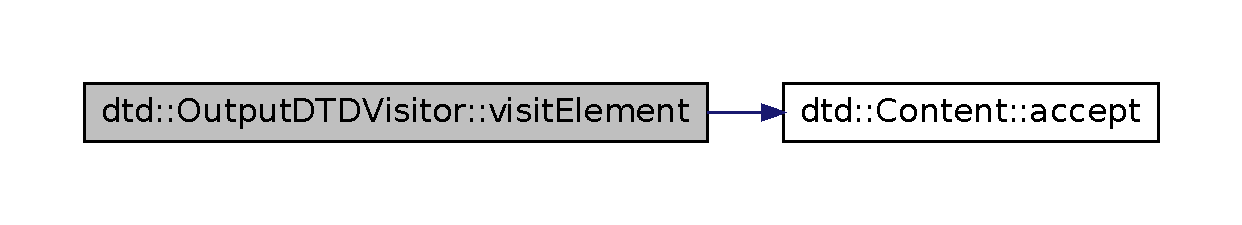
\includegraphics[width=400pt]{classdtd_1_1_output_d_t_d_visitor_ab95fcc93547eb5e038040f11b0f2b568_cgraph}
\end{center}
\end{figure}




\subsection{Documentation des données membres}
\hypertarget{classdtd_1_1_output_d_t_d_visitor_a8659c38013b7a5ba99e78c295a224362}{
\index{dtd::OutputDTDVisitor@{dtd::OutputDTDVisitor}!\_\-indent@{\_\-indent}}
\index{\_\-indent@{\_\-indent}!dtd::OutputDTDVisitor@{dtd::OutputDTDVisitor}}
\subsubsection[{\_\-indent}]{\setlength{\rightskip}{0pt plus 5cm}unsigned int {\bf dtd::OutputDTDVisitor::\_\-indent}\hspace{0.3cm}{\ttfamily  \mbox{[}protected\mbox{]}}}}
\label{classdtd_1_1_output_d_t_d_visitor_a8659c38013b7a5ba99e78c295a224362}


Définition à la ligne 79 du fichier OutputDTDVisitor.hh.

\hypertarget{classdtd_1_1_output_d_t_d_visitor_ae58e26bcaaa7c8681209a13934cea5f7}{
\index{dtd::OutputDTDVisitor@{dtd::OutputDTDVisitor}!\_\-indentChar@{\_\-indentChar}}
\index{\_\-indentChar@{\_\-indentChar}!dtd::OutputDTDVisitor@{dtd::OutputDTDVisitor}}
\subsubsection[{\_\-indentChar}]{\setlength{\rightskip}{0pt plus 5cm}char {\bf dtd::OutputDTDVisitor::\_\-indentChar}\hspace{0.3cm}{\ttfamily  \mbox{[}protected\mbox{]}}}}
\label{classdtd_1_1_output_d_t_d_visitor_ae58e26bcaaa7c8681209a13934cea5f7}


Définition à la ligne 77 du fichier OutputDTDVisitor.hh.

\hypertarget{classdtd_1_1_output_d_t_d_visitor_a913f11153a7fe38b61ff090d5bd99c89}{
\index{dtd::OutputDTDVisitor@{dtd::OutputDTDVisitor}!\_\-indentUnit@{\_\-indentUnit}}
\index{\_\-indentUnit@{\_\-indentUnit}!dtd::OutputDTDVisitor@{dtd::OutputDTDVisitor}}
\subsubsection[{\_\-indentUnit}]{\setlength{\rightskip}{0pt plus 5cm}unsigned {\bf dtd::OutputDTDVisitor::\_\-indentUnit}\hspace{0.3cm}{\ttfamily  \mbox{[}protected\mbox{]}}}}
\label{classdtd_1_1_output_d_t_d_visitor_a913f11153a7fe38b61ff090d5bd99c89}


Définition à la ligne 78 du fichier OutputDTDVisitor.hh.

\hypertarget{classdtd_1_1_output_d_t_d_visitor_a9a93007f2426887a2da46c30c5f2cc42}{
\index{dtd::OutputDTDVisitor@{dtd::OutputDTDVisitor}!\_\-out@{\_\-out}}
\index{\_\-out@{\_\-out}!dtd::OutputDTDVisitor@{dtd::OutputDTDVisitor}}
\subsubsection[{\_\-out}]{\setlength{\rightskip}{0pt plus 5cm}std::ostream\& {\bf dtd::OutputDTDVisitor::\_\-out}\hspace{0.3cm}{\ttfamily  \mbox{[}protected\mbox{]}}}}
\label{classdtd_1_1_output_d_t_d_visitor_a9a93007f2426887a2da46c30c5f2cc42}


Définition à la ligne 76 du fichier OutputDTDVisitor.hh.

\hypertarget{classdtd_1_1_output_d_t_d_visitor_a4f8609bcd2c8c20d1de80081835c48fc}{
\index{dtd::OutputDTDVisitor@{dtd::OutputDTDVisitor}!ANY\_\-CONTENT\_\-STR@{ANY\_\-CONTENT\_\-STR}}
\index{ANY\_\-CONTENT\_\-STR@{ANY\_\-CONTENT\_\-STR}!dtd::OutputDTDVisitor@{dtd::OutputDTDVisitor}}
\subsubsection[{ANY\_\-CONTENT\_\-STR}]{\setlength{\rightskip}{0pt plus 5cm}const std::string {\bf dtd::OutputDTDVisitor::ANY\_\-CONTENT\_\-STR} = \char`\"{}ANY\char`\"{}\hspace{0.3cm}{\ttfamily  \mbox{[}static, protected\mbox{]}}}}
\label{classdtd_1_1_output_d_t_d_visitor_a4f8609bcd2c8c20d1de80081835c48fc}


Définition à la ligne 69 du fichier OutputDTDVisitor.hh.

\hypertarget{classdtd_1_1_output_d_t_d_visitor_a4ce2c50f68b4f167879b57e970ca662c}{
\index{dtd::OutputDTDVisitor@{dtd::OutputDTDVisitor}!ATTLIST\_\-MARKUP\_\-NAME\_\-STR@{ATTLIST\_\-MARKUP\_\-NAME\_\-STR}}
\index{ATTLIST\_\-MARKUP\_\-NAME\_\-STR@{ATTLIST\_\-MARKUP\_\-NAME\_\-STR}!dtd::OutputDTDVisitor@{dtd::OutputDTDVisitor}}
\subsubsection[{ATTLIST\_\-MARKUP\_\-NAME\_\-STR}]{\setlength{\rightskip}{0pt plus 5cm}const std::string {\bf dtd::OutputDTDVisitor::ATTLIST\_\-MARKUP\_\-NAME\_\-STR} = \char`\"{}ATTLIST\char`\"{}\hspace{0.3cm}{\ttfamily  \mbox{[}static, protected\mbox{]}}}}
\label{classdtd_1_1_output_d_t_d_visitor_a4ce2c50f68b4f167879b57e970ca662c}


Définition à la ligne 57 du fichier OutputDTDVisitor.hh.

\hypertarget{classdtd_1_1_output_d_t_d_visitor_a686bb62aed37769865a688fe50e55f0a}{
\index{dtd::OutputDTDVisitor@{dtd::OutputDTDVisitor}!CHOICE\_\-SEPARATOR\_\-STR@{CHOICE\_\-SEPARATOR\_\-STR}}
\index{CHOICE\_\-SEPARATOR\_\-STR@{CHOICE\_\-SEPARATOR\_\-STR}!dtd::OutputDTDVisitor@{dtd::OutputDTDVisitor}}
\subsubsection[{CHOICE\_\-SEPARATOR\_\-STR}]{\setlength{\rightskip}{0pt plus 5cm}const std::string {\bf dtd::OutputDTDVisitor::CHOICE\_\-SEPARATOR\_\-STR} = \char`\"{}$|$\char`\"{}\hspace{0.3cm}{\ttfamily  \mbox{[}static, protected\mbox{]}}}}
\label{classdtd_1_1_output_d_t_d_visitor_a686bb62aed37769865a688fe50e55f0a}


Définition à la ligne 63 du fichier OutputDTDVisitor.hh.

\hypertarget{classdtd_1_1_output_d_t_d_visitor_a4dbe0d3fda6b73977f28488cf2f9cff4}{
\index{dtd::OutputDTDVisitor@{dtd::OutputDTDVisitor}!CLOSE\_\-MARKUP\_\-STR@{CLOSE\_\-MARKUP\_\-STR}}
\index{CLOSE\_\-MARKUP\_\-STR@{CLOSE\_\-MARKUP\_\-STR}!dtd::OutputDTDVisitor@{dtd::OutputDTDVisitor}}
\subsubsection[{CLOSE\_\-MARKUP\_\-STR}]{\setlength{\rightskip}{0pt plus 5cm}const std::string {\bf dtd::OutputDTDVisitor::CLOSE\_\-MARKUP\_\-STR} = \char`\"{}$>$\char`\"{}\hspace{0.3cm}{\ttfamily  \mbox{[}static, protected\mbox{]}}}}
\label{classdtd_1_1_output_d_t_d_visitor_a4dbe0d3fda6b73977f28488cf2f9cff4}


Définition à la ligne 74 du fichier OutputDTDVisitor.hh.

\hypertarget{classdtd_1_1_output_d_t_d_visitor_af8b2c8e68ec262f98a21334900cb09df}{
\index{dtd::OutputDTDVisitor@{dtd::OutputDTDVisitor}!DEFAULT\_\-INDENT\_\-CHAR@{DEFAULT\_\-INDENT\_\-CHAR}}
\index{DEFAULT\_\-INDENT\_\-CHAR@{DEFAULT\_\-INDENT\_\-CHAR}!dtd::OutputDTDVisitor@{dtd::OutputDTDVisitor}}
\subsubsection[{DEFAULT\_\-INDENT\_\-CHAR}]{\setlength{\rightskip}{0pt plus 5cm}const char {\bf dtd::OutputDTDVisitor::DEFAULT\_\-INDENT\_\-CHAR} = '$\backslash$t'\hspace{0.3cm}{\ttfamily  \mbox{[}static, protected\mbox{]}}}}
\label{classdtd_1_1_output_d_t_d_visitor_af8b2c8e68ec262f98a21334900cb09df}


Définition à la ligne 23 du fichier OutputDTDVisitor.hh.

\hypertarget{classdtd_1_1_output_d_t_d_visitor_a7795d56eeb6ab2e68c8d3a43e1c6f487}{
\index{dtd::OutputDTDVisitor@{dtd::OutputDTDVisitor}!DEFAULT\_\-INDENT\_\-UNIT@{DEFAULT\_\-INDENT\_\-UNIT}}
\index{DEFAULT\_\-INDENT\_\-UNIT@{DEFAULT\_\-INDENT\_\-UNIT}!dtd::OutputDTDVisitor@{dtd::OutputDTDVisitor}}
\subsubsection[{DEFAULT\_\-INDENT\_\-UNIT}]{\setlength{\rightskip}{0pt plus 5cm}const unsigned char {\bf dtd::OutputDTDVisitor::DEFAULT\_\-INDENT\_\-UNIT} = 1\hspace{0.3cm}{\ttfamily  \mbox{[}static, protected\mbox{]}}}}
\label{classdtd_1_1_output_d_t_d_visitor_a7795d56eeb6ab2e68c8d3a43e1c6f487}


Définition à la ligne 24 du fichier OutputDTDVisitor.hh.

\hypertarget{classdtd_1_1_output_d_t_d_visitor_a14cd0eb333af784f38e3441c8fd1b97d}{
\index{dtd::OutputDTDVisitor@{dtd::OutputDTDVisitor}!ELEMENT\_\-MARKUP\_\-NAME\_\-STR@{ELEMENT\_\-MARKUP\_\-NAME\_\-STR}}
\index{ELEMENT\_\-MARKUP\_\-NAME\_\-STR@{ELEMENT\_\-MARKUP\_\-NAME\_\-STR}!dtd::OutputDTDVisitor@{dtd::OutputDTDVisitor}}
\subsubsection[{ELEMENT\_\-MARKUP\_\-NAME\_\-STR}]{\setlength{\rightskip}{0pt plus 5cm}const std::string {\bf dtd::OutputDTDVisitor::ELEMENT\_\-MARKUP\_\-NAME\_\-STR} = \char`\"{}ELEMENT\char`\"{}\hspace{0.3cm}{\ttfamily  \mbox{[}static, protected\mbox{]}}}}
\label{classdtd_1_1_output_d_t_d_visitor_a14cd0eb333af784f38e3441c8fd1b97d}


Définition à la ligne 56 du fichier OutputDTDVisitor.hh.

\hypertarget{classdtd_1_1_output_d_t_d_visitor_af77ea7a3f4f05a3b3fea5a58a7d6de53}{
\index{dtd::OutputDTDVisitor@{dtd::OutputDTDVisitor}!EMPTY\_\-CONTENT\_\-STR@{EMPTY\_\-CONTENT\_\-STR}}
\index{EMPTY\_\-CONTENT\_\-STR@{EMPTY\_\-CONTENT\_\-STR}!dtd::OutputDTDVisitor@{dtd::OutputDTDVisitor}}
\subsubsection[{EMPTY\_\-CONTENT\_\-STR}]{\setlength{\rightskip}{0pt plus 5cm}const std::string {\bf dtd::OutputDTDVisitor::EMPTY\_\-CONTENT\_\-STR} = \char`\"{}EMPTY\char`\"{}\hspace{0.3cm}{\ttfamily  \mbox{[}static, protected\mbox{]}}}}
\label{classdtd_1_1_output_d_t_d_visitor_af77ea7a3f4f05a3b3fea5a58a7d6de53}


Définition à la ligne 68 du fichier OutputDTDVisitor.hh.

\hypertarget{classdtd_1_1_output_d_t_d_visitor_ab0306525af8ca54d3279c02a2d79da46}{
\index{dtd::OutputDTDVisitor@{dtd::OutputDTDVisitor}!END\_\-CHOICE\_\-STR@{END\_\-CHOICE\_\-STR}}
\index{END\_\-CHOICE\_\-STR@{END\_\-CHOICE\_\-STR}!dtd::OutputDTDVisitor@{dtd::OutputDTDVisitor}}
\subsubsection[{END\_\-CHOICE\_\-STR}]{\setlength{\rightskip}{0pt plus 5cm}const std::string {\bf dtd::OutputDTDVisitor::END\_\-CHOICE\_\-STR} = \char`\"{})\char`\"{}\hspace{0.3cm}{\ttfamily  \mbox{[}static, protected\mbox{]}}}}
\label{classdtd_1_1_output_d_t_d_visitor_ab0306525af8ca54d3279c02a2d79da46}


Définition à la ligne 64 du fichier OutputDTDVisitor.hh.

\hypertarget{classdtd_1_1_output_d_t_d_visitor_a217915df1bfe131dae99679461140fcc}{
\index{dtd::OutputDTDVisitor@{dtd::OutputDTDVisitor}!END\_\-MIXED\_\-STR@{END\_\-MIXED\_\-STR}}
\index{END\_\-MIXED\_\-STR@{END\_\-MIXED\_\-STR}!dtd::OutputDTDVisitor@{dtd::OutputDTDVisitor}}
\subsubsection[{END\_\-MIXED\_\-STR}]{\setlength{\rightskip}{0pt plus 5cm}const std::string {\bf dtd::OutputDTDVisitor::END\_\-MIXED\_\-STR} = \char`\"{})\char`\"{}\hspace{0.3cm}{\ttfamily  \mbox{[}static, protected\mbox{]}}}}
\label{classdtd_1_1_output_d_t_d_visitor_a217915df1bfe131dae99679461140fcc}


Définition à la ligne 67 du fichier OutputDTDVisitor.hh.

\hypertarget{classdtd_1_1_output_d_t_d_visitor_a17ea023b24838b7b2a96fe56a2c574ea}{
\index{dtd::OutputDTDVisitor@{dtd::OutputDTDVisitor}!END\_\-SEQUENCE\_\-STR@{END\_\-SEQUENCE\_\-STR}}
\index{END\_\-SEQUENCE\_\-STR@{END\_\-SEQUENCE\_\-STR}!dtd::OutputDTDVisitor@{dtd::OutputDTDVisitor}}
\subsubsection[{END\_\-SEQUENCE\_\-STR}]{\setlength{\rightskip}{0pt plus 5cm}const std::string {\bf dtd::OutputDTDVisitor::END\_\-SEQUENCE\_\-STR} = \char`\"{})\char`\"{}\hspace{0.3cm}{\ttfamily  \mbox{[}static, protected\mbox{]}}}}
\label{classdtd_1_1_output_d_t_d_visitor_a17ea023b24838b7b2a96fe56a2c574ea}


Définition à la ligne 61 du fichier OutputDTDVisitor.hh.

\hypertarget{classdtd_1_1_output_d_t_d_visitor_a32ceb547a079fa2498ff14d1aef6e112}{
\index{dtd::OutputDTDVisitor@{dtd::OutputDTDVisitor}!INSIDE\_\-MARKUP\_\-SPACE\_\-STR@{INSIDE\_\-MARKUP\_\-SPACE\_\-STR}}
\index{INSIDE\_\-MARKUP\_\-SPACE\_\-STR@{INSIDE\_\-MARKUP\_\-SPACE\_\-STR}!dtd::OutputDTDVisitor@{dtd::OutputDTDVisitor}}
\subsubsection[{INSIDE\_\-MARKUP\_\-SPACE\_\-STR}]{\setlength{\rightskip}{0pt plus 5cm}const std::string {\bf dtd::OutputDTDVisitor::INSIDE\_\-MARKUP\_\-SPACE\_\-STR} = \char`\"{} \char`\"{}\hspace{0.3cm}{\ttfamily  \mbox{[}static, protected\mbox{]}}}}
\label{classdtd_1_1_output_d_t_d_visitor_a32ceb547a079fa2498ff14d1aef6e112}


Définition à la ligne 58 du fichier OutputDTDVisitor.hh.

\hypertarget{classdtd_1_1_output_d_t_d_visitor_af583c776fabca5615d43da966dca600c}{
\index{dtd::OutputDTDVisitor@{dtd::OutputDTDVisitor}!MIXED\_\-SEPARATOR\_\-STR@{MIXED\_\-SEPARATOR\_\-STR}}
\index{MIXED\_\-SEPARATOR\_\-STR@{MIXED\_\-SEPARATOR\_\-STR}!dtd::OutputDTDVisitor@{dtd::OutputDTDVisitor}}
\subsubsection[{MIXED\_\-SEPARATOR\_\-STR}]{\setlength{\rightskip}{0pt plus 5cm}const std::string {\bf dtd::OutputDTDVisitor::MIXED\_\-SEPARATOR\_\-STR} = \char`\"{}$|$\char`\"{}\hspace{0.3cm}{\ttfamily  \mbox{[}static, protected\mbox{]}}}}
\label{classdtd_1_1_output_d_t_d_visitor_af583c776fabca5615d43da966dca600c}


Définition à la ligne 66 du fichier OutputDTDVisitor.hh.

\hypertarget{classdtd_1_1_output_d_t_d_visitor_aac75a1ed1d3189d021a65c5d56d1527e}{
\index{dtd::OutputDTDVisitor@{dtd::OutputDTDVisitor}!OPEN\_\-MARKUP\_\-STR@{OPEN\_\-MARKUP\_\-STR}}
\index{OPEN\_\-MARKUP\_\-STR@{OPEN\_\-MARKUP\_\-STR}!dtd::OutputDTDVisitor@{dtd::OutputDTDVisitor}}
\subsubsection[{OPEN\_\-MARKUP\_\-STR}]{\setlength{\rightskip}{0pt plus 5cm}const std::string {\bf dtd::OutputDTDVisitor::OPEN\_\-MARKUP\_\-STR} = \char`\"{}$<$!\char`\"{}\hspace{0.3cm}{\ttfamily  \mbox{[}static, protected\mbox{]}}}}
\label{classdtd_1_1_output_d_t_d_visitor_aac75a1ed1d3189d021a65c5d56d1527e}


Définition à la ligne 55 du fichier OutputDTDVisitor.hh.

\hypertarget{classdtd_1_1_output_d_t_d_visitor_a98f9105b5bccb426bc8a6e907a67b17f}{
\index{dtd::OutputDTDVisitor@{dtd::OutputDTDVisitor}!OPTIONAL\_\-QUANTIFIER\_\-STR@{OPTIONAL\_\-QUANTIFIER\_\-STR}}
\index{OPTIONAL\_\-QUANTIFIER\_\-STR@{OPTIONAL\_\-QUANTIFIER\_\-STR}!dtd::OutputDTDVisitor@{dtd::OutputDTDVisitor}}
\subsubsection[{OPTIONAL\_\-QUANTIFIER\_\-STR}]{\setlength{\rightskip}{0pt plus 5cm}const std::string {\bf dtd::OutputDTDVisitor::OPTIONAL\_\-QUANTIFIER\_\-STR} = \char`\"{}?\char`\"{}\hspace{0.3cm}{\ttfamily  \mbox{[}static, protected\mbox{]}}}}
\label{classdtd_1_1_output_d_t_d_visitor_a98f9105b5bccb426bc8a6e907a67b17f}


Définition à la ligne 71 du fichier OutputDTDVisitor.hh.

\hypertarget{classdtd_1_1_output_d_t_d_visitor_a4041af52751607ff7ae188484d962d95}{
\index{dtd::OutputDTDVisitor@{dtd::OutputDTDVisitor}!REPEATABLE\_\-QUANTIFIER\_\-STR@{REPEATABLE\_\-QUANTIFIER\_\-STR}}
\index{REPEATABLE\_\-QUANTIFIER\_\-STR@{REPEATABLE\_\-QUANTIFIER\_\-STR}!dtd::OutputDTDVisitor@{dtd::OutputDTDVisitor}}
\subsubsection[{REPEATABLE\_\-QUANTIFIER\_\-STR}]{\setlength{\rightskip}{0pt plus 5cm}const std::string {\bf dtd::OutputDTDVisitor::REPEATABLE\_\-QUANTIFIER\_\-STR} = \char`\"{}$\ast$\char`\"{}\hspace{0.3cm}{\ttfamily  \mbox{[}static, protected\mbox{]}}}}
\label{classdtd_1_1_output_d_t_d_visitor_a4041af52751607ff7ae188484d962d95}


Définition à la ligne 72 du fichier OutputDTDVisitor.hh.

\hypertarget{classdtd_1_1_output_d_t_d_visitor_ae8c6ec6c1f6ae17d8705be7267b07a2f}{
\index{dtd::OutputDTDVisitor@{dtd::OutputDTDVisitor}!REPEATED\_\-QUANTIFIER\_\-STR@{REPEATED\_\-QUANTIFIER\_\-STR}}
\index{REPEATED\_\-QUANTIFIER\_\-STR@{REPEATED\_\-QUANTIFIER\_\-STR}!dtd::OutputDTDVisitor@{dtd::OutputDTDVisitor}}
\subsubsection[{REPEATED\_\-QUANTIFIER\_\-STR}]{\setlength{\rightskip}{0pt plus 5cm}const std::string {\bf dtd::OutputDTDVisitor::REPEATED\_\-QUANTIFIER\_\-STR} = \char`\"{}+\char`\"{}\hspace{0.3cm}{\ttfamily  \mbox{[}static, protected\mbox{]}}}}
\label{classdtd_1_1_output_d_t_d_visitor_ae8c6ec6c1f6ae17d8705be7267b07a2f}


Définition à la ligne 73 du fichier OutputDTDVisitor.hh.

\hypertarget{classdtd_1_1_output_d_t_d_visitor_acfffbc0db723271579d1fd87dc699b05}{
\index{dtd::OutputDTDVisitor@{dtd::OutputDTDVisitor}!SEQUENCE\_\-SEPARATOR\_\-STR@{SEQUENCE\_\-SEPARATOR\_\-STR}}
\index{SEQUENCE\_\-SEPARATOR\_\-STR@{SEQUENCE\_\-SEPARATOR\_\-STR}!dtd::OutputDTDVisitor@{dtd::OutputDTDVisitor}}
\subsubsection[{SEQUENCE\_\-SEPARATOR\_\-STR}]{\setlength{\rightskip}{0pt plus 5cm}const std::string {\bf dtd::OutputDTDVisitor::SEQUENCE\_\-SEPARATOR\_\-STR} = \char`\"{},\char`\"{}\hspace{0.3cm}{\ttfamily  \mbox{[}static, protected\mbox{]}}}}
\label{classdtd_1_1_output_d_t_d_visitor_acfffbc0db723271579d1fd87dc699b05}


Définition à la ligne 60 du fichier OutputDTDVisitor.hh.

\hypertarget{classdtd_1_1_output_d_t_d_visitor_ae66777110076859a443e00a9da55ff1b}{
\index{dtd::OutputDTDVisitor@{dtd::OutputDTDVisitor}!START\_\-CHOICE\_\-STR@{START\_\-CHOICE\_\-STR}}
\index{START\_\-CHOICE\_\-STR@{START\_\-CHOICE\_\-STR}!dtd::OutputDTDVisitor@{dtd::OutputDTDVisitor}}
\subsubsection[{START\_\-CHOICE\_\-STR}]{\setlength{\rightskip}{0pt plus 5cm}const std::string {\bf dtd::OutputDTDVisitor::START\_\-CHOICE\_\-STR} = \char`\"{}(\char`\"{}\hspace{0.3cm}{\ttfamily  \mbox{[}static, protected\mbox{]}}}}
\label{classdtd_1_1_output_d_t_d_visitor_ae66777110076859a443e00a9da55ff1b}


Définition à la ligne 62 du fichier OutputDTDVisitor.hh.

\hypertarget{classdtd_1_1_output_d_t_d_visitor_a254da51819583f6fd4501521f741042d}{
\index{dtd::OutputDTDVisitor@{dtd::OutputDTDVisitor}!START\_\-MIXED\_\-STR@{START\_\-MIXED\_\-STR}}
\index{START\_\-MIXED\_\-STR@{START\_\-MIXED\_\-STR}!dtd::OutputDTDVisitor@{dtd::OutputDTDVisitor}}
\subsubsection[{START\_\-MIXED\_\-STR}]{\setlength{\rightskip}{0pt plus 5cm}const std::string {\bf dtd::OutputDTDVisitor::START\_\-MIXED\_\-STR} = \char`\"{}(\char`\"{}\hspace{0.3cm}{\ttfamily  \mbox{[}static, protected\mbox{]}}}}
\label{classdtd_1_1_output_d_t_d_visitor_a254da51819583f6fd4501521f741042d}


Définition à la ligne 65 du fichier OutputDTDVisitor.hh.

\hypertarget{classdtd_1_1_output_d_t_d_visitor_a1b325fb88f176ce92e566fe4e6423c1c}{
\index{dtd::OutputDTDVisitor@{dtd::OutputDTDVisitor}!START\_\-SEQUENCE\_\-STR@{START\_\-SEQUENCE\_\-STR}}
\index{START\_\-SEQUENCE\_\-STR@{START\_\-SEQUENCE\_\-STR}!dtd::OutputDTDVisitor@{dtd::OutputDTDVisitor}}
\subsubsection[{START\_\-SEQUENCE\_\-STR}]{\setlength{\rightskip}{0pt plus 5cm}const std::string {\bf dtd::OutputDTDVisitor::START\_\-SEQUENCE\_\-STR} = \char`\"{}(\char`\"{}\hspace{0.3cm}{\ttfamily  \mbox{[}static, protected\mbox{]}}}}
\label{classdtd_1_1_output_d_t_d_visitor_a1b325fb88f176ce92e566fe4e6423c1c}


Définition à la ligne 59 du fichier OutputDTDVisitor.hh.

\hypertarget{classdtd_1_1_output_d_t_d_visitor_a83f802e6ceef88d9496b0aedf4d4541e}{
\index{dtd::OutputDTDVisitor@{dtd::OutputDTDVisitor}!TEXT\_\-CONTENT\_\-STR@{TEXT\_\-CONTENT\_\-STR}}
\index{TEXT\_\-CONTENT\_\-STR@{TEXT\_\-CONTENT\_\-STR}!dtd::OutputDTDVisitor@{dtd::OutputDTDVisitor}}
\subsubsection[{TEXT\_\-CONTENT\_\-STR}]{\setlength{\rightskip}{0pt plus 5cm}const std::string {\bf dtd::OutputDTDVisitor::TEXT\_\-CONTENT\_\-STR} = \char`\"{}\#PCDATA\char`\"{}\hspace{0.3cm}{\ttfamily  \mbox{[}static, protected\mbox{]}}}}
\label{classdtd_1_1_output_d_t_d_visitor_a83f802e6ceef88d9496b0aedf4d4541e}


Définition à la ligne 70 du fichier OutputDTDVisitor.hh.



La documentation de cette classe a été générée à partir des fichiers suivants :\begin{DoxyCompactItemize}
\item 
src/\hyperlink{_output_d_t_d_visitor_8hh}{OutputDTDVisitor.hh}\item 
src/\hyperlink{_output_d_t_d_visitor_8cpp}{OutputDTDVisitor.cpp}\end{DoxyCompactItemize}

\hypertarget{classdtd_1_1_quantifiable_content}{
\section{Référence de la classe dtd::QuantifiableContent}
\label{classdtd_1_1_quantifiable_content}\index{dtd::QuantifiableContent@{dtd::QuantifiableContent}}
}


{\ttfamily \#include $<$QuantifiableContent.hh$>$}



Graphe d'héritage de dtd::QuantifiableContent:\nopagebreak
\begin{figure}[H]
\begin{center}
\leavevmode
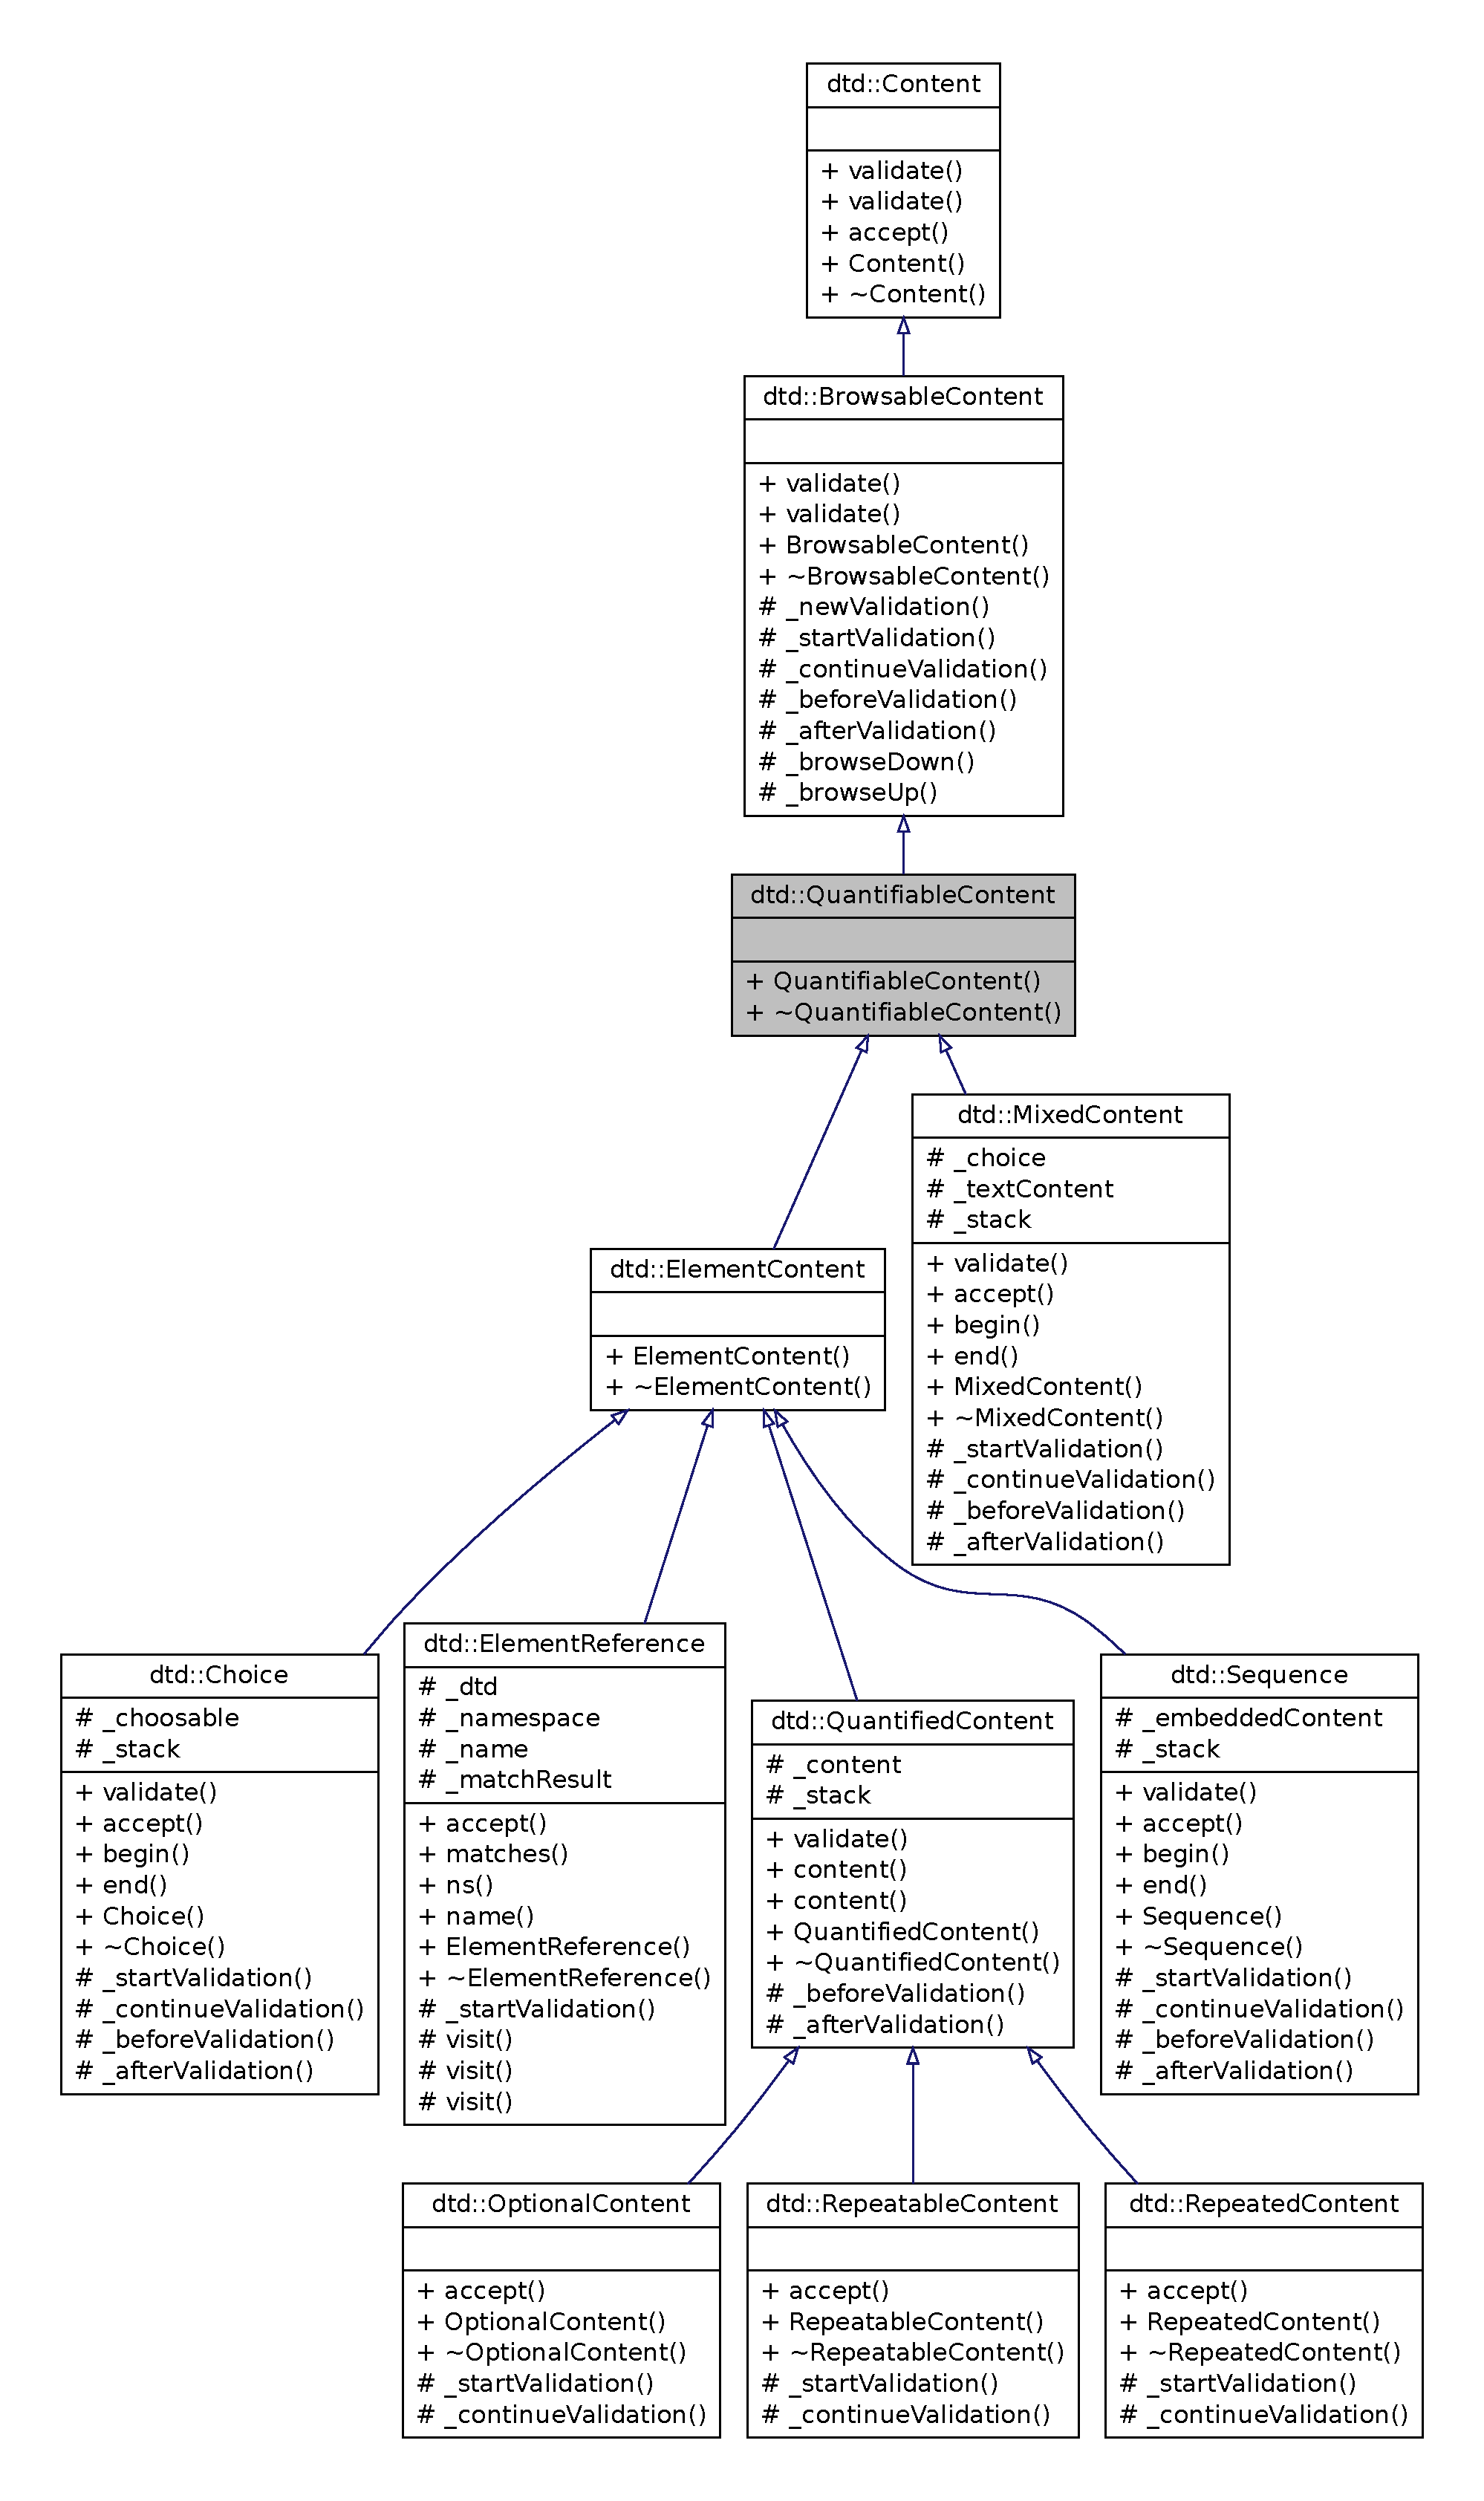
\includegraphics[height=600pt]{classdtd_1_1_quantifiable_content__inherit__graph}
\end{center}
\end{figure}


Graphe de collaboration de dtd::QuantifiableContent:\nopagebreak
\begin{figure}[H]
\begin{center}
\leavevmode
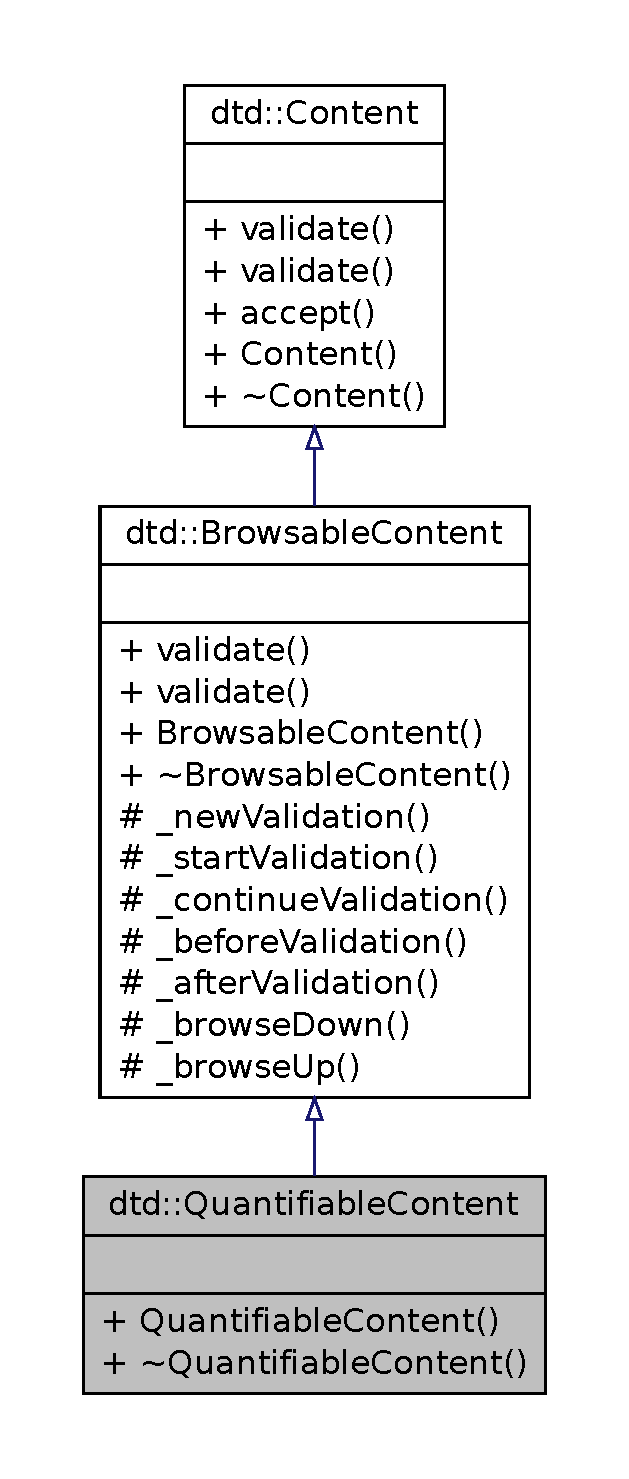
\includegraphics[height=600pt]{classdtd_1_1_quantifiable_content__coll__graph}
\end{center}
\end{figure}
\subsection*{Classes}
\begin{DoxyCompactItemize}
\item 
struct \hyperlink{structdtd_1_1_quantifiable_content_1_1___state}{\_\-State}
\end{DoxyCompactItemize}
\subsection*{Fonctions membres publiques}
\begin{DoxyCompactItemize}
\item 
\hyperlink{classdtd_1_1_quantifiable_content_a6ccde4e10b81f96ac9279bb53910e687}{QuantifiableContent} ()
\item 
virtual \hyperlink{classdtd_1_1_quantifiable_content_a67a1c9a8ca9877f574c08721fee8d268}{$\sim$QuantifiableContent} ()
\end{DoxyCompactItemize}


\subsection{Description détaillée}


Définition à la ligne 18 du fichier QuantifiableContent.hh.



\subsection{Documentation des constructeurs et destructeur}
\hypertarget{classdtd_1_1_quantifiable_content_a6ccde4e10b81f96ac9279bb53910e687}{
\index{dtd::QuantifiableContent@{dtd::QuantifiableContent}!QuantifiableContent@{QuantifiableContent}}
\index{QuantifiableContent@{QuantifiableContent}!dtd::QuantifiableContent@{dtd::QuantifiableContent}}
\subsubsection[{QuantifiableContent}]{\setlength{\rightskip}{0pt plus 5cm}dtd::QuantifiableContent::QuantifiableContent (
\begin{DoxyParamCaption}
{}
\end{DoxyParamCaption}
)}}
\label{classdtd_1_1_quantifiable_content_a6ccde4e10b81f96ac9279bb53910e687}


Définition à la ligne 36 du fichier QuantifiableContent.cpp.

\hypertarget{classdtd_1_1_quantifiable_content_a67a1c9a8ca9877f574c08721fee8d268}{
\index{dtd::QuantifiableContent@{dtd::QuantifiableContent}!$\sim$QuantifiableContent@{$\sim$QuantifiableContent}}
\index{$\sim$QuantifiableContent@{$\sim$QuantifiableContent}!dtd::QuantifiableContent@{dtd::QuantifiableContent}}
\subsubsection[{$\sim$QuantifiableContent}]{\setlength{\rightskip}{0pt plus 5cm}dtd::QuantifiableContent::$\sim$QuantifiableContent (
\begin{DoxyParamCaption}
{}
\end{DoxyParamCaption}
)\hspace{0.3cm}{\ttfamily  \mbox{[}virtual\mbox{]}}}}
\label{classdtd_1_1_quantifiable_content_a67a1c9a8ca9877f574c08721fee8d268}


Définition à la ligne 41 du fichier QuantifiableContent.cpp.



La documentation de cette classe a été générée à partir des fichiers suivants :\begin{DoxyCompactItemize}
\item 
src/\hyperlink{_quantifiable_content_8hh}{QuantifiableContent.hh}\item 
src/\hyperlink{_quantifiable_content_8cpp}{QuantifiableContent.cpp}\end{DoxyCompactItemize}

\hypertarget{classdtd_1_1_quantified_content}{
\section{Référence de la classe dtd::QuantifiedContent}
\label{classdtd_1_1_quantified_content}\index{dtd::QuantifiedContent@{dtd::QuantifiedContent}}
}


{\ttfamily \#include $<$QuantifiedContent.hh$>$}



Graphe d'héritage de dtd::QuantifiedContent:\nopagebreak
\begin{figure}[H]
\begin{center}
\leavevmode
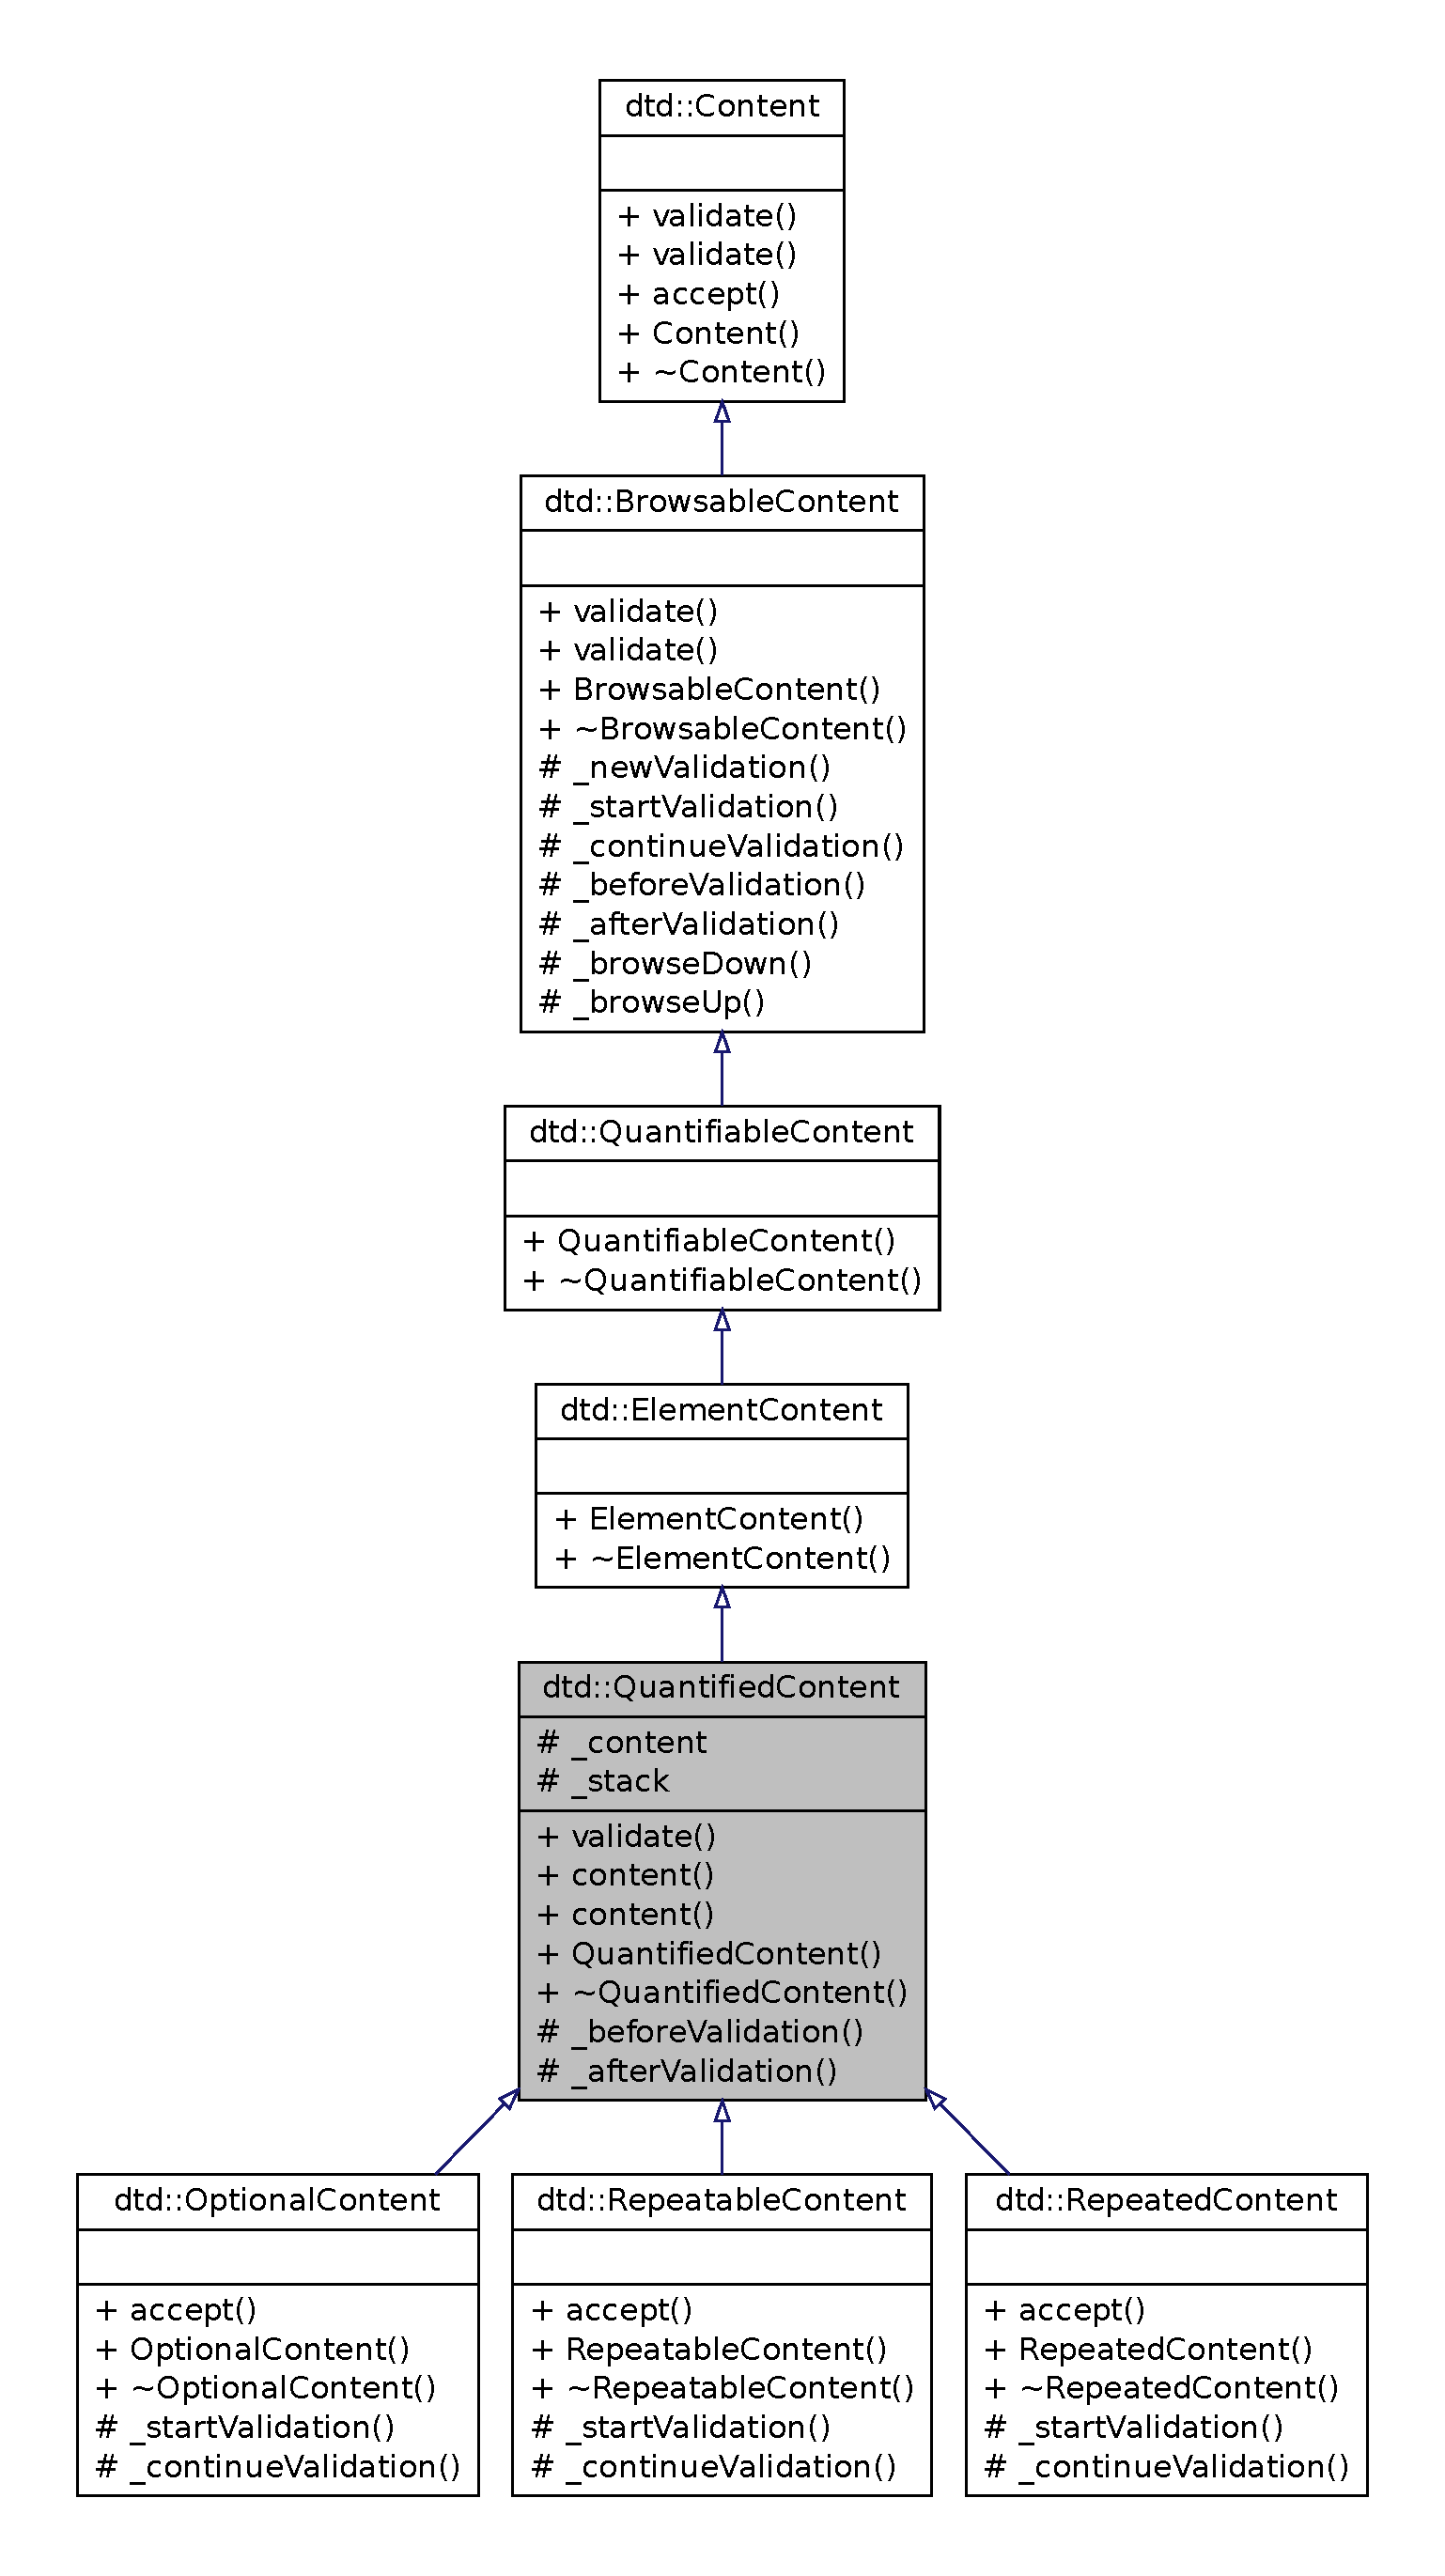
\includegraphics[height=600pt]{classdtd_1_1_quantified_content__inherit__graph}
\end{center}
\end{figure}


Graphe de collaboration de dtd::QuantifiedContent:\nopagebreak
\begin{figure}[H]
\begin{center}
\leavevmode
\includegraphics[height=600pt]{classdtd_1_1_quantified_content__coll__graph}
\end{center}
\end{figure}
\subsection*{Fonctions membres publiques}
\begin{DoxyCompactItemize}
\item 
virtual bool \hyperlink{classdtd_1_1_quantified_content_a83733f23442035bdbcd976723ed753a4}{validate} (const xml::CompositeMarkupNode \&node)
\item 
\hyperlink{classdtd_1_1_quantifiable_content}{QuantifiableContent} \& \hyperlink{classdtd_1_1_quantified_content_a5af034175edfa37f250b79b4c3ed3b92}{content} ()
\item 
const \hyperlink{classdtd_1_1_quantifiable_content}{QuantifiableContent} \& \hyperlink{classdtd_1_1_quantified_content_a29617e5aff808d66520c20626d673cae}{content} () const 
\item 
\hyperlink{classdtd_1_1_quantified_content_a687df58cee3795a5e47dfed39e6c6bf8}{QuantifiedContent} (\hyperlink{classdtd_1_1_quantifiable_content}{QuantifiableContent} \&content)
\item 
virtual \hyperlink{classdtd_1_1_quantified_content_ae67cf8463f4df5598acb62a0ffc06b39}{$\sim$QuantifiedContent} ()
\end{DoxyCompactItemize}
\subsection*{Types protégés}
\begin{DoxyCompactItemize}
\item 
typedef std::stack$<$ \hyperlink{structdtd_1_1_quantifiable_content_1_1___state}{\_\-State} $>$ \hyperlink{classdtd_1_1_quantified_content_af5a78d608bdaba704815995fbbe40f10}{\_\-StatesStack}
\end{DoxyCompactItemize}
\subsection*{Fonctions membres protégées}
\begin{DoxyCompactItemize}
\item 
virtual void \hyperlink{classdtd_1_1_quantified_content_a7be3fc2bcf3859567fd276e0d364b42e}{\_\-beforeValidation} (xml::CompositeMarkupNode::ChildrenIterator firstToken, xml::CompositeMarkupNode::ChildrenIterator endToken, \hyperlink{classdtd_1_1_browsable_content}{BrowsableContent} $\ast$nextStep)
\item 
virtual void \hyperlink{classdtd_1_1_quantified_content_a0830885ef44406a3ce571d8ad70fc014}{\_\-afterValidation} ()
\end{DoxyCompactItemize}
\subsection*{Attributs protégés}
\begin{DoxyCompactItemize}
\item 
\hyperlink{classdtd_1_1_quantifiable_content}{QuantifiableContent} \& \hyperlink{classdtd_1_1_quantified_content_a7372be0a6613cfb0795038937d73d321}{\_\-content}
\item 
\hyperlink{classdtd_1_1_quantified_content_af5a78d608bdaba704815995fbbe40f10}{\_\-StatesStack} \hyperlink{classdtd_1_1_quantified_content_acf63f34405d6c2b4016b442057fc0c56}{\_\-stack}
\end{DoxyCompactItemize}


\subsection{Description détaillée}


Définition à la ligne 19 du fichier QuantifiedContent.hh.



\subsection{Documentation des définitions de type membres}
\hypertarget{classdtd_1_1_quantified_content_af5a78d608bdaba704815995fbbe40f10}{
\index{dtd::QuantifiedContent@{dtd::QuantifiedContent}!\_\-StatesStack@{\_\-StatesStack}}
\index{\_\-StatesStack@{\_\-StatesStack}!dtd::QuantifiedContent@{dtd::QuantifiedContent}}
\subsubsection[{\_\-StatesStack}]{\setlength{\rightskip}{0pt plus 5cm}typedef std::stack$<${\bf \_\-State}$>$ {\bf dtd::QuantifiedContent::\_\-StatesStack}\hspace{0.3cm}{\ttfamily  \mbox{[}protected\mbox{]}}}}
\label{classdtd_1_1_quantified_content_af5a78d608bdaba704815995fbbe40f10}


Définition à la ligne 61 du fichier QuantifiedContent.hh.



\subsection{Documentation des constructeurs et destructeur}
\hypertarget{classdtd_1_1_quantified_content_a687df58cee3795a5e47dfed39e6c6bf8}{
\index{dtd::QuantifiedContent@{dtd::QuantifiedContent}!QuantifiedContent@{QuantifiedContent}}
\index{QuantifiedContent@{QuantifiedContent}!dtd::QuantifiedContent@{dtd::QuantifiedContent}}
\subsubsection[{QuantifiedContent}]{\setlength{\rightskip}{0pt plus 5cm}dtd::QuantifiedContent::QuantifiedContent (
\begin{DoxyParamCaption}
\item[{{\bf QuantifiableContent} \&}]{ content}
\end{DoxyParamCaption}
)}}
\label{classdtd_1_1_quantified_content_a687df58cee3795a5e47dfed39e6c6bf8}


Définition à la ligne 53 du fichier QuantifiedContent.cpp.

\hypertarget{classdtd_1_1_quantified_content_ae67cf8463f4df5598acb62a0ffc06b39}{
\index{dtd::QuantifiedContent@{dtd::QuantifiedContent}!$\sim$QuantifiedContent@{$\sim$QuantifiedContent}}
\index{$\sim$QuantifiedContent@{$\sim$QuantifiedContent}!dtd::QuantifiedContent@{dtd::QuantifiedContent}}
\subsubsection[{$\sim$QuantifiedContent}]{\setlength{\rightskip}{0pt plus 5cm}dtd::QuantifiedContent::$\sim$QuantifiedContent (
\begin{DoxyParamCaption}
{}
\end{DoxyParamCaption}
)\hspace{0.3cm}{\ttfamily  \mbox{[}virtual\mbox{]}}}}
\label{classdtd_1_1_quantified_content_ae67cf8463f4df5598acb62a0ffc06b39}


Définition à la ligne 59 du fichier QuantifiedContent.cpp.



\subsection{Documentation des fonctions membres}
\hypertarget{classdtd_1_1_quantified_content_a0830885ef44406a3ce571d8ad70fc014}{
\index{dtd::QuantifiedContent@{dtd::QuantifiedContent}!\_\-afterValidation@{\_\-afterValidation}}
\index{\_\-afterValidation@{\_\-afterValidation}!dtd::QuantifiedContent@{dtd::QuantifiedContent}}
\subsubsection[{\_\-afterValidation}]{\setlength{\rightskip}{0pt plus 5cm}void dtd::QuantifiedContent::\_\-afterValidation (
\begin{DoxyParamCaption}
{}
\end{DoxyParamCaption}
)\hspace{0.3cm}{\ttfamily  \mbox{[}protected, virtual\mbox{]}}}}
\label{classdtd_1_1_quantified_content_a0830885ef44406a3ce571d8ad70fc014}


Réimplémentée à partir de \hyperlink{classdtd_1_1_browsable_content_a378fc620af75eb9bad9f37c663e3838d}{dtd::BrowsableContent}.



Définition à la ligne 75 du fichier QuantifiedContent.cpp.

\hypertarget{classdtd_1_1_quantified_content_a7be3fc2bcf3859567fd276e0d364b42e}{
\index{dtd::QuantifiedContent@{dtd::QuantifiedContent}!\_\-beforeValidation@{\_\-beforeValidation}}
\index{\_\-beforeValidation@{\_\-beforeValidation}!dtd::QuantifiedContent@{dtd::QuantifiedContent}}
\subsubsection[{\_\-beforeValidation}]{\setlength{\rightskip}{0pt plus 5cm}void dtd::QuantifiedContent::\_\-beforeValidation (
\begin{DoxyParamCaption}
\item[{xml::CompositeMarkupNode::ChildrenIterator}]{ firstToken, }
\item[{xml::CompositeMarkupNode::ChildrenIterator}]{ endToken, }
\item[{{\bf BrowsableContent} $\ast$}]{ nextStep}
\end{DoxyParamCaption}
)\hspace{0.3cm}{\ttfamily  \mbox{[}protected, virtual\mbox{]}}}}
\label{classdtd_1_1_quantified_content_a7be3fc2bcf3859567fd276e0d364b42e}


Réimplémentée à partir de \hyperlink{classdtd_1_1_browsable_content_ae9e55da18cc09557fc7896a7ccac2ee1}{dtd::BrowsableContent}.



Définition à la ligne 67 du fichier QuantifiedContent.cpp.

\hypertarget{classdtd_1_1_quantified_content_a5af034175edfa37f250b79b4c3ed3b92}{
\index{dtd::QuantifiedContent@{dtd::QuantifiedContent}!content@{content}}
\index{content@{content}!dtd::QuantifiedContent@{dtd::QuantifiedContent}}
\subsubsection[{content}]{\setlength{\rightskip}{0pt plus 5cm}{\bf QuantifiableContent} \& dtd::QuantifiedContent::content (
\begin{DoxyParamCaption}
{}
\end{DoxyParamCaption}
)}}
\label{classdtd_1_1_quantified_content_a5af034175edfa37f250b79b4c3ed3b92}


Définition à la ligne 39 du fichier QuantifiedContent.cpp.

\hypertarget{classdtd_1_1_quantified_content_a29617e5aff808d66520c20626d673cae}{
\index{dtd::QuantifiedContent@{dtd::QuantifiedContent}!content@{content}}
\index{content@{content}!dtd::QuantifiedContent@{dtd::QuantifiedContent}}
\subsubsection[{content}]{\setlength{\rightskip}{0pt plus 5cm}const {\bf QuantifiableContent} \& dtd::QuantifiedContent::content (
\begin{DoxyParamCaption}
{}
\end{DoxyParamCaption}
) const}}
\label{classdtd_1_1_quantified_content_a29617e5aff808d66520c20626d673cae}


Définition à la ligne 44 du fichier QuantifiedContent.cpp.

\hypertarget{classdtd_1_1_quantified_content_a83733f23442035bdbcd976723ed753a4}{
\index{dtd::QuantifiedContent@{dtd::QuantifiedContent}!validate@{validate}}
\index{validate@{validate}!dtd::QuantifiedContent@{dtd::QuantifiedContent}}
\subsubsection[{validate}]{\setlength{\rightskip}{0pt plus 5cm}virtual bool dtd::QuantifiedContent::validate (
\begin{DoxyParamCaption}
\item[{const xml::CompositeMarkupNode \&}]{ node}
\end{DoxyParamCaption}
)\hspace{0.3cm}{\ttfamily  \mbox{[}virtual\mbox{]}}}}
\label{classdtd_1_1_quantified_content_a83733f23442035bdbcd976723ed753a4}


Réimplémentée à partir de \hyperlink{classdtd_1_1_browsable_content_a824a0c41b66aeea689e4283ee453d398}{dtd::BrowsableContent}.



\subsection{Documentation des données membres}
\hypertarget{classdtd_1_1_quantified_content_a7372be0a6613cfb0795038937d73d321}{
\index{dtd::QuantifiedContent@{dtd::QuantifiedContent}!\_\-content@{\_\-content}}
\index{\_\-content@{\_\-content}!dtd::QuantifiedContent@{dtd::QuantifiedContent}}
\subsubsection[{\_\-content}]{\setlength{\rightskip}{0pt plus 5cm}{\bf QuantifiableContent}\& {\bf dtd::QuantifiedContent::\_\-content}\hspace{0.3cm}{\ttfamily  \mbox{[}protected\mbox{]}}}}
\label{classdtd_1_1_quantified_content_a7372be0a6613cfb0795038937d73d321}


Définition à la ligne 59 du fichier QuantifiedContent.hh.

\hypertarget{classdtd_1_1_quantified_content_acf63f34405d6c2b4016b442057fc0c56}{
\index{dtd::QuantifiedContent@{dtd::QuantifiedContent}!\_\-stack@{\_\-stack}}
\index{\_\-stack@{\_\-stack}!dtd::QuantifiedContent@{dtd::QuantifiedContent}}
\subsubsection[{\_\-stack}]{\setlength{\rightskip}{0pt plus 5cm}{\bf \_\-StatesStack} {\bf dtd::QuantifiedContent::\_\-stack}\hspace{0.3cm}{\ttfamily  \mbox{[}protected\mbox{]}}}}
\label{classdtd_1_1_quantified_content_acf63f34405d6c2b4016b442057fc0c56}


Définition à la ligne 62 du fichier QuantifiedContent.hh.



La documentation de cette classe a été générée à partir des fichiers suivants :\begin{DoxyCompactItemize}
\item 
src/\hyperlink{_quantified_content_8hh}{QuantifiedContent.hh}\item 
src/\hyperlink{_quantified_content_8cpp}{QuantifiedContent.cpp}\end{DoxyCompactItemize}

\hypertarget{classdtd_1_1_repeatable_content}{
\section{Référence de la classe dtd::RepeatableContent}
\label{classdtd_1_1_repeatable_content}\index{dtd::RepeatableContent@{dtd::RepeatableContent}}
}


{\ttfamily \#include $<$RepeatableContent.hh$>$}



Graphe d'héritage de dtd::RepeatableContent:\nopagebreak
\begin{figure}[H]
\begin{center}
\leavevmode
\includegraphics[height=600pt]{classdtd_1_1_repeatable_content__inherit__graph}
\end{center}
\end{figure}


Graphe de collaboration de dtd::RepeatableContent:\nopagebreak
\begin{figure}[H]
\begin{center}
\leavevmode
\includegraphics[height=600pt]{classdtd_1_1_repeatable_content__coll__graph}
\end{center}
\end{figure}
\subsection*{Fonctions membres publiques}
\begin{DoxyCompactItemize}
\item 
virtual void \hyperlink{classdtd_1_1_repeatable_content_a28550745ec781816e4be44165dbb3934}{accept} (\hyperlink{classdtd_1_1_interface_d_t_d_visitor}{InterfaceDTDVisitor} \&visitor) const 
\item 
\hyperlink{classdtd_1_1_repeatable_content_a5aa05c57a86876a8f23420ac7df42de6}{RepeatableContent} (\hyperlink{classdtd_1_1_quantifiable_content}{QuantifiableContent} \&content)
\item 
virtual \hyperlink{classdtd_1_1_repeatable_content_a2eec6b242d0ef49af02f530405fb3525}{$\sim$RepeatableContent} ()
\end{DoxyCompactItemize}
\subsection*{Fonctions membres protégées}
\begin{DoxyCompactItemize}
\item 
virtual bool \hyperlink{classdtd_1_1_repeatable_content_aa71e67d3e836b9ee0edc856c8dbc5f47}{\_\-startValidation} (xml::CompositeMarkupNode::ChildrenIterator firstToken, xml::CompositeMarkupNode::ChildrenIterator endToken, \hyperlink{classdtd_1_1_browsable_content}{BrowsableContent} $\ast$nextStep)
\item 
virtual bool \hyperlink{classdtd_1_1_repeatable_content_af7cda09f207d691feec9846d757910c3}{\_\-continueValidation} (xml::CompositeMarkupNode::ChildrenIterator currentToken)
\end{DoxyCompactItemize}


\subsection{Description détaillée}


Définition à la ligne 18 du fichier RepeatableContent.hh.



\subsection{Documentation des constructeurs et destructeur}
\hypertarget{classdtd_1_1_repeatable_content_a5aa05c57a86876a8f23420ac7df42de6}{
\index{dtd::RepeatableContent@{dtd::RepeatableContent}!RepeatableContent@{RepeatableContent}}
\index{RepeatableContent@{RepeatableContent}!dtd::RepeatableContent@{dtd::RepeatableContent}}
\subsubsection[{RepeatableContent}]{\setlength{\rightskip}{0pt plus 5cm}dtd::RepeatableContent::RepeatableContent (
\begin{DoxyParamCaption}
\item[{{\bf QuantifiableContent} \&}]{ content}
\end{DoxyParamCaption}
)}}
\label{classdtd_1_1_repeatable_content_a5aa05c57a86876a8f23420ac7df42de6}


Définition à la ligne 42 du fichier RepeatableContent.cpp.

\hypertarget{classdtd_1_1_repeatable_content_a2eec6b242d0ef49af02f530405fb3525}{
\index{dtd::RepeatableContent@{dtd::RepeatableContent}!$\sim$RepeatableContent@{$\sim$RepeatableContent}}
\index{$\sim$RepeatableContent@{$\sim$RepeatableContent}!dtd::RepeatableContent@{dtd::RepeatableContent}}
\subsubsection[{$\sim$RepeatableContent}]{\setlength{\rightskip}{0pt plus 5cm}dtd::RepeatableContent::$\sim$RepeatableContent (
\begin{DoxyParamCaption}
{}
\end{DoxyParamCaption}
)\hspace{0.3cm}{\ttfamily  \mbox{[}virtual\mbox{]}}}}
\label{classdtd_1_1_repeatable_content_a2eec6b242d0ef49af02f530405fb3525}


Définition à la ligne 48 du fichier RepeatableContent.cpp.



\subsection{Documentation des fonctions membres}
\hypertarget{classdtd_1_1_repeatable_content_af7cda09f207d691feec9846d757910c3}{
\index{dtd::RepeatableContent@{dtd::RepeatableContent}!\_\-continueValidation@{\_\-continueValidation}}
\index{\_\-continueValidation@{\_\-continueValidation}!dtd::RepeatableContent@{dtd::RepeatableContent}}
\subsubsection[{\_\-continueValidation}]{\setlength{\rightskip}{0pt plus 5cm}bool dtd::RepeatableContent::\_\-continueValidation (
\begin{DoxyParamCaption}
\item[{xml::CompositeMarkupNode::ChildrenIterator}]{ currentToken}
\end{DoxyParamCaption}
)\hspace{0.3cm}{\ttfamily  \mbox{[}protected, virtual\mbox{]}}}}
\label{classdtd_1_1_repeatable_content_af7cda09f207d691feec9846d757910c3}


Réimplémentée à partir de \hyperlink{classdtd_1_1_browsable_content_a6398e5990648e2af3fd775592b0d62ea}{dtd::BrowsableContent}.



Définition à la ligne 67 du fichier RepeatableContent.cpp.



Voici le graphe d'appel pour cette fonction :\nopagebreak
\begin{figure}[H]
\begin{center}
\leavevmode
\includegraphics[width=400pt]{classdtd_1_1_repeatable_content_af7cda09f207d691feec9846d757910c3_cgraph}
\end{center}
\end{figure}


\hypertarget{classdtd_1_1_repeatable_content_aa71e67d3e836b9ee0edc856c8dbc5f47}{
\index{dtd::RepeatableContent@{dtd::RepeatableContent}!\_\-startValidation@{\_\-startValidation}}
\index{\_\-startValidation@{\_\-startValidation}!dtd::RepeatableContent@{dtd::RepeatableContent}}
\subsubsection[{\_\-startValidation}]{\setlength{\rightskip}{0pt plus 5cm}virtual bool dtd::RepeatableContent::\_\-startValidation (
\begin{DoxyParamCaption}
\item[{xml::CompositeMarkupNode::ChildrenIterator}]{ firstToken, }
\item[{xml::CompositeMarkupNode::ChildrenIterator}]{ endToken, }
\item[{{\bf BrowsableContent} $\ast$}]{ nextStep}
\end{DoxyParamCaption}
)\hspace{0.3cm}{\ttfamily  \mbox{[}protected, virtual\mbox{]}}}}
\label{classdtd_1_1_repeatable_content_aa71e67d3e836b9ee0edc856c8dbc5f47}


Implémente \hyperlink{classdtd_1_1_browsable_content_a67ab5a7329d94e363796ae2d17617246}{dtd::BrowsableContent}.

\hypertarget{classdtd_1_1_repeatable_content_a28550745ec781816e4be44165dbb3934}{
\index{dtd::RepeatableContent@{dtd::RepeatableContent}!accept@{accept}}
\index{accept@{accept}!dtd::RepeatableContent@{dtd::RepeatableContent}}
\subsubsection[{accept}]{\setlength{\rightskip}{0pt plus 5cm}void dtd::RepeatableContent::accept (
\begin{DoxyParamCaption}
\item[{{\bf InterfaceDTDVisitor} \&}]{ visitor}
\end{DoxyParamCaption}
) const\hspace{0.3cm}{\ttfamily  \mbox{[}virtual\mbox{]}}}}
\label{classdtd_1_1_repeatable_content_a28550745ec781816e4be44165dbb3934}


Implémente \hyperlink{classdtd_1_1_content_a403cc15f12eaa187ad493fa600540cd8}{dtd::Content}.



Définition à la ligne 33 du fichier RepeatableContent.cpp.



Voici le graphe d'appel pour cette fonction :\nopagebreak
\begin{figure}[H]
\begin{center}
\leavevmode
\includegraphics[width=400pt]{classdtd_1_1_repeatable_content_a28550745ec781816e4be44165dbb3934_cgraph}
\end{center}
\end{figure}




La documentation de cette classe a été générée à partir des fichiers suivants :\begin{DoxyCompactItemize}
\item 
src/\hyperlink{_repeatable_content_8hh}{RepeatableContent.hh}\item 
src/\hyperlink{_repeatable_content_8cpp}{RepeatableContent.cpp}\end{DoxyCompactItemize}

\hypertarget{classdtd_1_1_repeated_content}{
\section{Référence de la classe dtd::RepeatedContent}
\label{classdtd_1_1_repeated_content}\index{dtd::RepeatedContent@{dtd::RepeatedContent}}
}


{\ttfamily \#include $<$RepeatedContent.hh$>$}



Graphe d'héritage de dtd::RepeatedContent:\nopagebreak
\begin{figure}[H]
\begin{center}
\leavevmode
\includegraphics[height=600pt]{classdtd_1_1_repeated_content__inherit__graph}
\end{center}
\end{figure}


Graphe de collaboration de dtd::RepeatedContent:\nopagebreak
\begin{figure}[H]
\begin{center}
\leavevmode
\includegraphics[height=600pt]{classdtd_1_1_repeated_content__coll__graph}
\end{center}
\end{figure}
\subsection*{Fonctions membres publiques}
\begin{DoxyCompactItemize}
\item 
virtual void \hyperlink{classdtd_1_1_repeated_content_af97dd8df71c00b1ec91d577671c8ed77}{accept} (\hyperlink{classdtd_1_1_interface_d_t_d_visitor}{InterfaceDTDVisitor} \&visitor) const 
\item 
\hyperlink{classdtd_1_1_repeated_content_a05f44a98e9d27becfd1690c9638fe339}{RepeatedContent} (\hyperlink{classdtd_1_1_quantifiable_content}{QuantifiableContent} \&content)
\item 
virtual \hyperlink{classdtd_1_1_repeated_content_afd585386d77a53f9bba1507a5fd58c6f}{$\sim$RepeatedContent} ()
\end{DoxyCompactItemize}
\subsection*{Fonctions membres protégées}
\begin{DoxyCompactItemize}
\item 
virtual bool \hyperlink{classdtd_1_1_repeated_content_a3202c603a2cc800b6cbaf32880745dd3}{\_\-startValidation} (xml::CompositeMarkupNode::ChildrenIterator firstToken, xml::CompositeMarkupNode::ChildrenIterator endToken, \hyperlink{classdtd_1_1_browsable_content}{BrowsableContent} $\ast$nextStep)
\item 
virtual bool \hyperlink{classdtd_1_1_repeated_content_a3c3b6ab6dec9c12044e56198fc492db0}{\_\-continueValidation} (xml::CompositeMarkupNode::ChildrenIterator currentToken)
\end{DoxyCompactItemize}


\subsection{Description détaillée}


Définition à la ligne 18 du fichier RepeatedContent.hh.



\subsection{Documentation des constructeurs et destructeur}
\hypertarget{classdtd_1_1_repeated_content_a05f44a98e9d27becfd1690c9638fe339}{
\index{dtd::RepeatedContent@{dtd::RepeatedContent}!RepeatedContent@{RepeatedContent}}
\index{RepeatedContent@{RepeatedContent}!dtd::RepeatedContent@{dtd::RepeatedContent}}
\subsubsection[{RepeatedContent}]{\setlength{\rightskip}{0pt plus 5cm}dtd::RepeatedContent::RepeatedContent (
\begin{DoxyParamCaption}
\item[{{\bf QuantifiableContent} \&}]{ content}
\end{DoxyParamCaption}
)}}
\label{classdtd_1_1_repeated_content_a05f44a98e9d27becfd1690c9638fe339}


Définition à la ligne 42 du fichier RepeatedContent.cpp.

\hypertarget{classdtd_1_1_repeated_content_afd585386d77a53f9bba1507a5fd58c6f}{
\index{dtd::RepeatedContent@{dtd::RepeatedContent}!$\sim$RepeatedContent@{$\sim$RepeatedContent}}
\index{$\sim$RepeatedContent@{$\sim$RepeatedContent}!dtd::RepeatedContent@{dtd::RepeatedContent}}
\subsubsection[{$\sim$RepeatedContent}]{\setlength{\rightskip}{0pt plus 5cm}dtd::RepeatedContent::$\sim$RepeatedContent (
\begin{DoxyParamCaption}
{}
\end{DoxyParamCaption}
)\hspace{0.3cm}{\ttfamily  \mbox{[}virtual\mbox{]}}}}
\label{classdtd_1_1_repeated_content_afd585386d77a53f9bba1507a5fd58c6f}


Définition à la ligne 48 du fichier RepeatedContent.cpp.



\subsection{Documentation des fonctions membres}
\hypertarget{classdtd_1_1_repeated_content_a3c3b6ab6dec9c12044e56198fc492db0}{
\index{dtd::RepeatedContent@{dtd::RepeatedContent}!\_\-continueValidation@{\_\-continueValidation}}
\index{\_\-continueValidation@{\_\-continueValidation}!dtd::RepeatedContent@{dtd::RepeatedContent}}
\subsubsection[{\_\-continueValidation}]{\setlength{\rightskip}{0pt plus 5cm}bool dtd::RepeatedContent::\_\-continueValidation (
\begin{DoxyParamCaption}
\item[{xml::CompositeMarkupNode::ChildrenIterator}]{ currentToken}
\end{DoxyParamCaption}
)\hspace{0.3cm}{\ttfamily  \mbox{[}protected, virtual\mbox{]}}}}
\label{classdtd_1_1_repeated_content_a3c3b6ab6dec9c12044e56198fc492db0}


Réimplémentée à partir de \hyperlink{classdtd_1_1_browsable_content_a6398e5990648e2af3fd775592b0d62ea}{dtd::BrowsableContent}.



Définition à la ligne 65 du fichier RepeatedContent.cpp.



Voici le graphe d'appel pour cette fonction :\nopagebreak
\begin{figure}[H]
\begin{center}
\leavevmode
\includegraphics[width=400pt]{classdtd_1_1_repeated_content_a3c3b6ab6dec9c12044e56198fc492db0_cgraph}
\end{center}
\end{figure}


\hypertarget{classdtd_1_1_repeated_content_a3202c603a2cc800b6cbaf32880745dd3}{
\index{dtd::RepeatedContent@{dtd::RepeatedContent}!\_\-startValidation@{\_\-startValidation}}
\index{\_\-startValidation@{\_\-startValidation}!dtd::RepeatedContent@{dtd::RepeatedContent}}
\subsubsection[{\_\-startValidation}]{\setlength{\rightskip}{0pt plus 5cm}virtual bool dtd::RepeatedContent::\_\-startValidation (
\begin{DoxyParamCaption}
\item[{xml::CompositeMarkupNode::ChildrenIterator}]{ firstToken, }
\item[{xml::CompositeMarkupNode::ChildrenIterator}]{ endToken, }
\item[{{\bf BrowsableContent} $\ast$}]{ nextStep}
\end{DoxyParamCaption}
)\hspace{0.3cm}{\ttfamily  \mbox{[}protected, virtual\mbox{]}}}}
\label{classdtd_1_1_repeated_content_a3202c603a2cc800b6cbaf32880745dd3}


Implémente \hyperlink{classdtd_1_1_browsable_content_a67ab5a7329d94e363796ae2d17617246}{dtd::BrowsableContent}.

\hypertarget{classdtd_1_1_repeated_content_af97dd8df71c00b1ec91d577671c8ed77}{
\index{dtd::RepeatedContent@{dtd::RepeatedContent}!accept@{accept}}
\index{accept@{accept}!dtd::RepeatedContent@{dtd::RepeatedContent}}
\subsubsection[{accept}]{\setlength{\rightskip}{0pt plus 5cm}void dtd::RepeatedContent::accept (
\begin{DoxyParamCaption}
\item[{{\bf InterfaceDTDVisitor} \&}]{ visitor}
\end{DoxyParamCaption}
) const\hspace{0.3cm}{\ttfamily  \mbox{[}virtual\mbox{]}}}}
\label{classdtd_1_1_repeated_content_af97dd8df71c00b1ec91d577671c8ed77}


Implémente \hyperlink{classdtd_1_1_content_a403cc15f12eaa187ad493fa600540cd8}{dtd::Content}.



Définition à la ligne 33 du fichier RepeatedContent.cpp.



Voici le graphe d'appel pour cette fonction :\nopagebreak
\begin{figure}[H]
\begin{center}
\leavevmode
\includegraphics[width=400pt]{classdtd_1_1_repeated_content_af97dd8df71c00b1ec91d577671c8ed77_cgraph}
\end{center}
\end{figure}




La documentation de cette classe a été générée à partir des fichiers suivants :\begin{DoxyCompactItemize}
\item 
src/\hyperlink{_repeated_content_8hh}{RepeatedContent.hh}\item 
src/\hyperlink{_repeated_content_8cpp}{RepeatedContent.cpp}\end{DoxyCompactItemize}

\hypertarget{classdtd_1_1_sequence}{
\section{Référence de la classe dtd::Sequence}
\label{classdtd_1_1_sequence}\index{dtd::Sequence@{dtd::Sequence}}
}


{\ttfamily \#include $<$Sequence.hh$>$}



Graphe d'héritage de dtd::Sequence:\nopagebreak
\begin{figure}[H]
\begin{center}
\leavevmode
\includegraphics[height=600pt]{classdtd_1_1_sequence__inherit__graph}
\end{center}
\end{figure}


Graphe de collaboration de dtd::Sequence:\nopagebreak
\begin{figure}[H]
\begin{center}
\leavevmode
\includegraphics[height=600pt]{classdtd_1_1_sequence__coll__graph}
\end{center}
\end{figure}
\subsection*{Classes}
\begin{DoxyCompactItemize}
\item 
struct \hyperlink{structdtd_1_1_sequence_1_1___state}{\_\-State}
\end{DoxyCompactItemize}
\subsection*{Types publics}
\begin{DoxyCompactItemize}
\item 
typedef std::list$<$ \hyperlink{classdtd_1_1_element_content}{ElementContent} $\ast$ $>$ \hyperlink{classdtd_1_1_sequence_a0bb035768b3473ac3ba35a2a019ef67a}{OrderedContent}
\item 
typedef \_\-OrderedContent::const\_\-iterator \hyperlink{classdtd_1_1_sequence_a497ef84646eebfccfb0b47ca526dd5cd}{const\_\-iterator}
\end{DoxyCompactItemize}
\subsection*{Fonctions membres publiques}
\begin{DoxyCompactItemize}
\item 
virtual bool \hyperlink{classdtd_1_1_sequence_a585eecddf1104ba42a15944ee4ff4b19}{validate} (const xml::CompositeMarkupNode \&node)
\item 
virtual void \hyperlink{classdtd_1_1_sequence_aa7ce2af63b36ed8be694d875488b108a}{accept} (\hyperlink{classdtd_1_1_interface_d_t_d_visitor}{InterfaceDTDVisitor} \&visitor) const 
\item 
\hyperlink{classdtd_1_1_sequence_a497ef84646eebfccfb0b47ca526dd5cd}{const\_\-iterator} \hyperlink{classdtd_1_1_sequence_ae8a6613ea98f553fdb265509a83935ed}{begin} () const 
\item 
\hyperlink{classdtd_1_1_sequence_a497ef84646eebfccfb0b47ca526dd5cd}{const\_\-iterator} \hyperlink{classdtd_1_1_sequence_a2419c3cfce9678c6f3e9848681d708b2}{end} () const 
\item 
\hyperlink{classdtd_1_1_sequence_ad6a2ad60f2706ccbdd1b6d1720a14ad5}{Sequence} (const \hyperlink{classdtd_1_1_sequence_a0bb035768b3473ac3ba35a2a019ef67a}{OrderedContent} \&embeddedContent)
\item 
virtual \hyperlink{classdtd_1_1_sequence_a119c90cd0d58c42c58acac2e9fa51c54}{$\sim$Sequence} ()
\end{DoxyCompactItemize}
\subsection*{Types protégés}
\begin{DoxyCompactItemize}
\item 
typedef std::list$<$ \hyperlink{classdtd_1_1_element_content}{ElementContent} $\ast$ $>$ \hyperlink{classdtd_1_1_sequence_ae8f07ee87cfe7be8dd9eb5bf01959d66}{\_\-OrderedContent}
\item 
typedef std::stack$<$ \hyperlink{structdtd_1_1_quantifiable_content_1_1___state}{\_\-State} $>$ \hyperlink{classdtd_1_1_sequence_a779e1658dfabe1973ec9a2524501bc88}{\_\-StatesStack}
\end{DoxyCompactItemize}
\subsection*{Fonctions membres protégées}
\begin{DoxyCompactItemize}
\item 
virtual bool \hyperlink{classdtd_1_1_sequence_a2765bc73d7fa4b92fafd60611e56e0f3}{\_\-startValidation} (xml::CompositeMarkupNode::ChildrenIterator firstToken, xml::CompositeMarkupNode::ChildrenIterator endToken, \hyperlink{classdtd_1_1_browsable_content}{BrowsableContent} $\ast$nextStep)
\item 
virtual bool \hyperlink{classdtd_1_1_sequence_a02874d51ebf3777a7fd16ee0e70b523b}{\_\-continueValidation} (xml::CompositeMarkupNode::ChildrenIterator currentToken)
\item 
virtual void \hyperlink{classdtd_1_1_sequence_a249219a1b47cc8298277491fe8356434}{\_\-beforeValidation} (xml::CompositeMarkupNode::ChildrenIterator firstToken, xml::CompositeMarkupNode::ChildrenIterator endToken, \hyperlink{classdtd_1_1_browsable_content}{BrowsableContent} $\ast$nextStep)
\item 
virtual void \hyperlink{classdtd_1_1_sequence_a9ab781006b7163a87e9b6d7e46314727}{\_\-afterValidation} ()
\end{DoxyCompactItemize}
\subsection*{Attributs protégés}
\begin{DoxyCompactItemize}
\item 
\hyperlink{classdtd_1_1_sequence_ae8f07ee87cfe7be8dd9eb5bf01959d66}{\_\-OrderedContent} \hyperlink{classdtd_1_1_sequence_a36b690d5fe1490780c079cb65f9821f6}{\_\-embeddedContent}
\item 
\hyperlink{classdtd_1_1_sequence_a779e1658dfabe1973ec9a2524501bc88}{\_\-StatesStack} \hyperlink{classdtd_1_1_sequence_aa0d3d57604b1b62caeb0eb2c7b776169}{\_\-stack}
\end{DoxyCompactItemize}


\subsection{Description détaillée}


Définition à la ligne 20 du fichier Sequence.hh.



\subsection{Documentation des définitions de type membres}
\hypertarget{classdtd_1_1_sequence_ae8f07ee87cfe7be8dd9eb5bf01959d66}{
\index{dtd::Sequence@{dtd::Sequence}!\_\-OrderedContent@{\_\-OrderedContent}}
\index{\_\-OrderedContent@{\_\-OrderedContent}!dtd::Sequence@{dtd::Sequence}}
\subsubsection[{\_\-OrderedContent}]{\setlength{\rightskip}{0pt plus 5cm}typedef std::list$<${\bf ElementContent}$\ast$$>$ {\bf dtd::Sequence::\_\-OrderedContent}\hspace{0.3cm}{\ttfamily  \mbox{[}protected\mbox{]}}}}
\label{classdtd_1_1_sequence_ae8f07ee87cfe7be8dd9eb5bf01959d66}


Définition à la ligne 23 du fichier Sequence.hh.

\hypertarget{classdtd_1_1_sequence_a779e1658dfabe1973ec9a2524501bc88}{
\index{dtd::Sequence@{dtd::Sequence}!\_\-StatesStack@{\_\-StatesStack}}
\index{\_\-StatesStack@{\_\-StatesStack}!dtd::Sequence@{dtd::Sequence}}
\subsubsection[{\_\-StatesStack}]{\setlength{\rightskip}{0pt plus 5cm}typedef std::stack$<${\bf \_\-State}$>$ {\bf dtd::Sequence::\_\-StatesStack}\hspace{0.3cm}{\ttfamily  \mbox{[}protected\mbox{]}}}}
\label{classdtd_1_1_sequence_a779e1658dfabe1973ec9a2524501bc88}


Définition à la ligne 97 du fichier Sequence.hh.

\hypertarget{classdtd_1_1_sequence_a497ef84646eebfccfb0b47ca526dd5cd}{
\index{dtd::Sequence@{dtd::Sequence}!const\_\-iterator@{const\_\-iterator}}
\index{const\_\-iterator@{const\_\-iterator}!dtd::Sequence@{dtd::Sequence}}
\subsubsection[{const\_\-iterator}]{\setlength{\rightskip}{0pt plus 5cm}typedef \_\-OrderedContent::const\_\-iterator {\bf dtd::Sequence::const\_\-iterator}}}
\label{classdtd_1_1_sequence_a497ef84646eebfccfb0b47ca526dd5cd}


Définition à la ligne 29 du fichier Sequence.hh.

\hypertarget{classdtd_1_1_sequence_a0bb035768b3473ac3ba35a2a019ef67a}{
\index{dtd::Sequence@{dtd::Sequence}!OrderedContent@{OrderedContent}}
\index{OrderedContent@{OrderedContent}!dtd::Sequence@{dtd::Sequence}}
\subsubsection[{OrderedContent}]{\setlength{\rightskip}{0pt plus 5cm}typedef std::list$<${\bf ElementContent}$\ast$$>$ {\bf dtd::Sequence::OrderedContent}}}
\label{classdtd_1_1_sequence_a0bb035768b3473ac3ba35a2a019ef67a}


Définition à la ligne 28 du fichier Sequence.hh.



\subsection{Documentation des constructeurs et destructeur}
\hypertarget{classdtd_1_1_sequence_ad6a2ad60f2706ccbdd1b6d1720a14ad5}{
\index{dtd::Sequence@{dtd::Sequence}!Sequence@{Sequence}}
\index{Sequence@{Sequence}!dtd::Sequence@{dtd::Sequence}}
\subsubsection[{Sequence}]{\setlength{\rightskip}{0pt plus 5cm}dtd::Sequence::Sequence (
\begin{DoxyParamCaption}
\item[{const {\bf OrderedContent} \&}]{ embeddedContent}
\end{DoxyParamCaption}
)}}
\label{classdtd_1_1_sequence_ad6a2ad60f2706ccbdd1b6d1720a14ad5}


Définition à la ligne 61 du fichier Sequence.cpp.

\hypertarget{classdtd_1_1_sequence_a119c90cd0d58c42c58acac2e9fa51c54}{
\index{dtd::Sequence@{dtd::Sequence}!$\sim$Sequence@{$\sim$Sequence}}
\index{$\sim$Sequence@{$\sim$Sequence}!dtd::Sequence@{dtd::Sequence}}
\subsubsection[{$\sim$Sequence}]{\setlength{\rightskip}{0pt plus 5cm}dtd::Sequence::$\sim$Sequence (
\begin{DoxyParamCaption}
{}
\end{DoxyParamCaption}
)\hspace{0.3cm}{\ttfamily  \mbox{[}virtual\mbox{]}}}}
\label{classdtd_1_1_sequence_a119c90cd0d58c42c58acac2e9fa51c54}


Définition à la ligne 67 du fichier Sequence.cpp.



\subsection{Documentation des fonctions membres}
\hypertarget{classdtd_1_1_sequence_a9ab781006b7163a87e9b6d7e46314727}{
\index{dtd::Sequence@{dtd::Sequence}!\_\-afterValidation@{\_\-afterValidation}}
\index{\_\-afterValidation@{\_\-afterValidation}!dtd::Sequence@{dtd::Sequence}}
\subsubsection[{\_\-afterValidation}]{\setlength{\rightskip}{0pt plus 5cm}void dtd::Sequence::\_\-afterValidation (
\begin{DoxyParamCaption}
{}
\end{DoxyParamCaption}
)\hspace{0.3cm}{\ttfamily  \mbox{[}protected, virtual\mbox{]}}}}
\label{classdtd_1_1_sequence_a9ab781006b7163a87e9b6d7e46314727}


Réimplémentée à partir de \hyperlink{classdtd_1_1_browsable_content_a378fc620af75eb9bad9f37c663e3838d}{dtd::BrowsableContent}.



Définition à la ligne 88 du fichier Sequence.cpp.

\hypertarget{classdtd_1_1_sequence_a249219a1b47cc8298277491fe8356434}{
\index{dtd::Sequence@{dtd::Sequence}!\_\-beforeValidation@{\_\-beforeValidation}}
\index{\_\-beforeValidation@{\_\-beforeValidation}!dtd::Sequence@{dtd::Sequence}}
\subsubsection[{\_\-beforeValidation}]{\setlength{\rightskip}{0pt plus 5cm}void dtd::Sequence::\_\-beforeValidation (
\begin{DoxyParamCaption}
\item[{xml::CompositeMarkupNode::ChildrenIterator}]{ firstToken, }
\item[{xml::CompositeMarkupNode::ChildrenIterator}]{ endToken, }
\item[{{\bf BrowsableContent} $\ast$}]{ nextStep}
\end{DoxyParamCaption}
)\hspace{0.3cm}{\ttfamily  \mbox{[}protected, virtual\mbox{]}}}}
\label{classdtd_1_1_sequence_a249219a1b47cc8298277491fe8356434}


Réimplémentée à partir de \hyperlink{classdtd_1_1_browsable_content_ae9e55da18cc09557fc7896a7ccac2ee1}{dtd::BrowsableContent}.



Définition à la ligne 79 du fichier Sequence.cpp.

\hypertarget{classdtd_1_1_sequence_a02874d51ebf3777a7fd16ee0e70b523b}{
\index{dtd::Sequence@{dtd::Sequence}!\_\-continueValidation@{\_\-continueValidation}}
\index{\_\-continueValidation@{\_\-continueValidation}!dtd::Sequence@{dtd::Sequence}}
\subsubsection[{\_\-continueValidation}]{\setlength{\rightskip}{0pt plus 5cm}bool dtd::Sequence::\_\-continueValidation (
\begin{DoxyParamCaption}
\item[{xml::CompositeMarkupNode::ChildrenIterator}]{ currentToken}
\end{DoxyParamCaption}
)\hspace{0.3cm}{\ttfamily  \mbox{[}protected, virtual\mbox{]}}}}
\label{classdtd_1_1_sequence_a02874d51ebf3777a7fd16ee0e70b523b}


Réimplémentée à partir de \hyperlink{classdtd_1_1_browsable_content_a6398e5990648e2af3fd775592b0d62ea}{dtd::BrowsableContent}.



Définition à la ligne 102 du fichier Sequence.cpp.



Voici le graphe d'appel pour cette fonction :\nopagebreak
\begin{figure}[H]
\begin{center}
\leavevmode
\includegraphics[width=400pt]{classdtd_1_1_sequence_a02874d51ebf3777a7fd16ee0e70b523b_cgraph}
\end{center}
\end{figure}


\hypertarget{classdtd_1_1_sequence_a2765bc73d7fa4b92fafd60611e56e0f3}{
\index{dtd::Sequence@{dtd::Sequence}!\_\-startValidation@{\_\-startValidation}}
\index{\_\-startValidation@{\_\-startValidation}!dtd::Sequence@{dtd::Sequence}}
\subsubsection[{\_\-startValidation}]{\setlength{\rightskip}{0pt plus 5cm}virtual bool dtd::Sequence::\_\-startValidation (
\begin{DoxyParamCaption}
\item[{xml::CompositeMarkupNode::ChildrenIterator}]{ firstToken, }
\item[{xml::CompositeMarkupNode::ChildrenIterator}]{ endToken, }
\item[{{\bf BrowsableContent} $\ast$}]{ nextStep}
\end{DoxyParamCaption}
)\hspace{0.3cm}{\ttfamily  \mbox{[}protected, virtual\mbox{]}}}}
\label{classdtd_1_1_sequence_a2765bc73d7fa4b92fafd60611e56e0f3}


Implémente \hyperlink{classdtd_1_1_browsable_content_a67ab5a7329d94e363796ae2d17617246}{dtd::BrowsableContent}.

\hypertarget{classdtd_1_1_sequence_aa7ce2af63b36ed8be694d875488b108a}{
\index{dtd::Sequence@{dtd::Sequence}!accept@{accept}}
\index{accept@{accept}!dtd::Sequence@{dtd::Sequence}}
\subsubsection[{accept}]{\setlength{\rightskip}{0pt plus 5cm}void dtd::Sequence::accept (
\begin{DoxyParamCaption}
\item[{{\bf InterfaceDTDVisitor} \&}]{ visitor}
\end{DoxyParamCaption}
) const\hspace{0.3cm}{\ttfamily  \mbox{[}virtual\mbox{]}}}}
\label{classdtd_1_1_sequence_aa7ce2af63b36ed8be694d875488b108a}


Implémente \hyperlink{classdtd_1_1_content_a403cc15f12eaa187ad493fa600540cd8}{dtd::Content}.



Définition à la ligne 41 du fichier Sequence.cpp.



Voici le graphe d'appel pour cette fonction :\nopagebreak
\begin{figure}[H]
\begin{center}
\leavevmode
\includegraphics[width=400pt]{classdtd_1_1_sequence_aa7ce2af63b36ed8be694d875488b108a_cgraph}
\end{center}
\end{figure}


\hypertarget{classdtd_1_1_sequence_ae8a6613ea98f553fdb265509a83935ed}{
\index{dtd::Sequence@{dtd::Sequence}!begin@{begin}}
\index{begin@{begin}!dtd::Sequence@{dtd::Sequence}}
\subsubsection[{begin}]{\setlength{\rightskip}{0pt plus 5cm}{\bf Sequence::const\_\-iterator} dtd::Sequence::begin (
\begin{DoxyParamCaption}
{}
\end{DoxyParamCaption}
) const}}
\label{classdtd_1_1_sequence_ae8a6613ea98f553fdb265509a83935ed}


Définition à la ligne 46 du fichier Sequence.cpp.

\hypertarget{classdtd_1_1_sequence_a2419c3cfce9678c6f3e9848681d708b2}{
\index{dtd::Sequence@{dtd::Sequence}!end@{end}}
\index{end@{end}!dtd::Sequence@{dtd::Sequence}}
\subsubsection[{end}]{\setlength{\rightskip}{0pt plus 5cm}{\bf Sequence::const\_\-iterator} dtd::Sequence::end (
\begin{DoxyParamCaption}
{}
\end{DoxyParamCaption}
) const}}
\label{classdtd_1_1_sequence_a2419c3cfce9678c6f3e9848681d708b2}


Définition à la ligne 51 du fichier Sequence.cpp.

\hypertarget{classdtd_1_1_sequence_a585eecddf1104ba42a15944ee4ff4b19}{
\index{dtd::Sequence@{dtd::Sequence}!validate@{validate}}
\index{validate@{validate}!dtd::Sequence@{dtd::Sequence}}
\subsubsection[{validate}]{\setlength{\rightskip}{0pt plus 5cm}virtual bool dtd::Sequence::validate (
\begin{DoxyParamCaption}
\item[{const xml::CompositeMarkupNode \&}]{ node}
\end{DoxyParamCaption}
)\hspace{0.3cm}{\ttfamily  \mbox{[}virtual\mbox{]}}}}
\label{classdtd_1_1_sequence_a585eecddf1104ba42a15944ee4ff4b19}


Réimplémentée à partir de \hyperlink{classdtd_1_1_browsable_content_a824a0c41b66aeea689e4283ee453d398}{dtd::BrowsableContent}.



\subsection{Documentation des données membres}
\hypertarget{classdtd_1_1_sequence_a36b690d5fe1490780c079cb65f9821f6}{
\index{dtd::Sequence@{dtd::Sequence}!\_\-embeddedContent@{\_\-embeddedContent}}
\index{\_\-embeddedContent@{\_\-embeddedContent}!dtd::Sequence@{dtd::Sequence}}
\subsubsection[{\_\-embeddedContent}]{\setlength{\rightskip}{0pt plus 5cm}{\bf \_\-OrderedContent} {\bf dtd::Sequence::\_\-embeddedContent}\hspace{0.3cm}{\ttfamily  \mbox{[}protected\mbox{]}}}}
\label{classdtd_1_1_sequence_a36b690d5fe1490780c079cb65f9821f6}


Définition à la ligne 81 du fichier Sequence.hh.

\hypertarget{classdtd_1_1_sequence_aa0d3d57604b1b62caeb0eb2c7b776169}{
\index{dtd::Sequence@{dtd::Sequence}!\_\-stack@{\_\-stack}}
\index{\_\-stack@{\_\-stack}!dtd::Sequence@{dtd::Sequence}}
\subsubsection[{\_\-stack}]{\setlength{\rightskip}{0pt plus 5cm}{\bf \_\-StatesStack} {\bf dtd::Sequence::\_\-stack}\hspace{0.3cm}{\ttfamily  \mbox{[}protected\mbox{]}}}}
\label{classdtd_1_1_sequence_aa0d3d57604b1b62caeb0eb2c7b776169}


Définition à la ligne 98 du fichier Sequence.hh.



La documentation de cette classe a été générée à partir des fichiers suivants :\begin{DoxyCompactItemize}
\item 
src/\hyperlink{_sequence_8hh}{Sequence.hh}\item 
src/\hyperlink{_sequence_8cpp}{Sequence.cpp}\end{DoxyCompactItemize}

\hypertarget{classdtd_1_1_text_content}{
\section{Référence de la classe dtd::TextContent}
\label{classdtd_1_1_text_content}\index{dtd::TextContent@{dtd::TextContent}}
}


{\ttfamily \#include $<$TextContent.hh$>$}



Graphe d'héritage de dtd::TextContent:\nopagebreak
\begin{figure}[H]
\begin{center}
\leavevmode
\includegraphics[height=600pt]{classdtd_1_1_text_content__inherit__graph}
\end{center}
\end{figure}


Graphe de collaboration de dtd::TextContent:\nopagebreak
\begin{figure}[H]
\begin{center}
\leavevmode
\includegraphics[height=600pt]{classdtd_1_1_text_content__coll__graph}
\end{center}
\end{figure}
\subsection*{Fonctions membres publiques}
\begin{DoxyCompactItemize}
\item 
virtual void \hyperlink{classdtd_1_1_text_content_a5193fbafe92665d975b886a6ca18ac4f}{accept} (\hyperlink{classdtd_1_1_interface_d_t_d_visitor}{InterfaceDTDVisitor} \&visitor) const 
\item 
\hyperlink{classdtd_1_1_text_content_a20db379cdb659e237de428f1ae0c4a16}{TextContent} ()
\item 
virtual \hyperlink{classdtd_1_1_text_content_aec396d8d7dcf1808ee05291f3cc77104}{$\sim$TextContent} ()
\end{DoxyCompactItemize}
\subsection*{Fonctions membres protégées}
\begin{DoxyCompactItemize}
\item 
virtual bool \hyperlink{classdtd_1_1_text_content_aa1f8d36777cd6b71686ee4db19268ae6}{\_\-startValidation} (xml::CompositeMarkupNode::ChildrenIterator firstToken, xml::CompositeMarkupNode::ChildrenIterator endToken, \hyperlink{classdtd_1_1_browsable_content}{BrowsableContent} $\ast$nextStep)
\item 
virtual void \hyperlink{classdtd_1_1_text_content_a26e7bd6531bc9733286a63fc0089637e}{visit} (const xml::TextNode \&node)
\item 
virtual void \hyperlink{classdtd_1_1_text_content_a10dbfd9abf5f8b7a8bd15175d95de51e}{visit} (const xml::MarkupNode \&node)
\item 
virtual void \hyperlink{classdtd_1_1_text_content_adf1c22f7d497842044f9a6a2f2e53a00}{visit} (const xml::CompositeMarkupNode \&node)
\end{DoxyCompactItemize}
\subsection*{Attributs protégés}
\begin{DoxyCompactItemize}
\item 
bool \hyperlink{classdtd_1_1_text_content_a8aed746e0439c19af52a4b844a05e1b4}{\_\-validationResult}
\end{DoxyCompactItemize}


\subsection{Description détaillée}


Définition à la ligne 19 du fichier TextContent.hh.



\subsection{Documentation des constructeurs et destructeur}
\hypertarget{classdtd_1_1_text_content_a20db379cdb659e237de428f1ae0c4a16}{
\index{dtd::TextContent@{dtd::TextContent}!TextContent@{TextContent}}
\index{TextContent@{TextContent}!dtd::TextContent@{dtd::TextContent}}
\subsubsection[{TextContent}]{\setlength{\rightskip}{0pt plus 5cm}dtd::TextContent::TextContent (
\begin{DoxyParamCaption}
{}
\end{DoxyParamCaption}
)}}
\label{classdtd_1_1_text_content_a20db379cdb659e237de428f1ae0c4a16}


Définition à la ligne 42 du fichier TextContent.cpp.

\hypertarget{classdtd_1_1_text_content_aec396d8d7dcf1808ee05291f3cc77104}{
\index{dtd::TextContent@{dtd::TextContent}!$\sim$TextContent@{$\sim$TextContent}}
\index{$\sim$TextContent@{$\sim$TextContent}!dtd::TextContent@{dtd::TextContent}}
\subsubsection[{$\sim$TextContent}]{\setlength{\rightskip}{0pt plus 5cm}dtd::TextContent::$\sim$TextContent (
\begin{DoxyParamCaption}
{}
\end{DoxyParamCaption}
)\hspace{0.3cm}{\ttfamily  \mbox{[}virtual\mbox{]}}}}
\label{classdtd_1_1_text_content_aec396d8d7dcf1808ee05291f3cc77104}


Définition à la ligne 47 du fichier TextContent.cpp.



\subsection{Documentation des fonctions membres}
\hypertarget{classdtd_1_1_text_content_aa1f8d36777cd6b71686ee4db19268ae6}{
\index{dtd::TextContent@{dtd::TextContent}!\_\-startValidation@{\_\-startValidation}}
\index{\_\-startValidation@{\_\-startValidation}!dtd::TextContent@{dtd::TextContent}}
\subsubsection[{\_\-startValidation}]{\setlength{\rightskip}{0pt plus 5cm}virtual bool dtd::TextContent::\_\-startValidation (
\begin{DoxyParamCaption}
\item[{xml::CompositeMarkupNode::ChildrenIterator}]{ firstToken, }
\item[{xml::CompositeMarkupNode::ChildrenIterator}]{ endToken, }
\item[{{\bf BrowsableContent} $\ast$}]{ nextStep}
\end{DoxyParamCaption}
)\hspace{0.3cm}{\ttfamily  \mbox{[}protected, virtual\mbox{]}}}}
\label{classdtd_1_1_text_content_aa1f8d36777cd6b71686ee4db19268ae6}


Implémente \hyperlink{classdtd_1_1_browsable_content_a67ab5a7329d94e363796ae2d17617246}{dtd::BrowsableContent}.

\hypertarget{classdtd_1_1_text_content_a5193fbafe92665d975b886a6ca18ac4f}{
\index{dtd::TextContent@{dtd::TextContent}!accept@{accept}}
\index{accept@{accept}!dtd::TextContent@{dtd::TextContent}}
\subsubsection[{accept}]{\setlength{\rightskip}{0pt plus 5cm}void dtd::TextContent::accept (
\begin{DoxyParamCaption}
\item[{{\bf InterfaceDTDVisitor} \&}]{ visitor}
\end{DoxyParamCaption}
) const\hspace{0.3cm}{\ttfamily  \mbox{[}virtual\mbox{]}}}}
\label{classdtd_1_1_text_content_a5193fbafe92665d975b886a6ca18ac4f}


Implémente \hyperlink{classdtd_1_1_content_a403cc15f12eaa187ad493fa600540cd8}{dtd::Content}.



Définition à la ligne 33 du fichier TextContent.cpp.



Voici le graphe d'appel pour cette fonction :\nopagebreak
\begin{figure}[H]
\begin{center}
\leavevmode
\includegraphics[width=400pt]{classdtd_1_1_text_content_a5193fbafe92665d975b886a6ca18ac4f_cgraph}
\end{center}
\end{figure}


\hypertarget{classdtd_1_1_text_content_a10dbfd9abf5f8b7a8bd15175d95de51e}{
\index{dtd::TextContent@{dtd::TextContent}!visit@{visit}}
\index{visit@{visit}!dtd::TextContent@{dtd::TextContent}}
\subsubsection[{visit}]{\setlength{\rightskip}{0pt plus 5cm}virtual void dtd::TextContent::visit (
\begin{DoxyParamCaption}
\item[{const xml::MarkupNode \&}]{ node}
\end{DoxyParamCaption}
)\hspace{0.3cm}{\ttfamily  \mbox{[}protected, virtual\mbox{]}}}}
\label{classdtd_1_1_text_content_a10dbfd9abf5f8b7a8bd15175d95de51e}
\hypertarget{classdtd_1_1_text_content_a26e7bd6531bc9733286a63fc0089637e}{
\index{dtd::TextContent@{dtd::TextContent}!visit@{visit}}
\index{visit@{visit}!dtd::TextContent@{dtd::TextContent}}
\subsubsection[{visit}]{\setlength{\rightskip}{0pt plus 5cm}virtual void dtd::TextContent::visit (
\begin{DoxyParamCaption}
\item[{const xml::TextNode \&}]{ node}
\end{DoxyParamCaption}
)\hspace{0.3cm}{\ttfamily  \mbox{[}protected, virtual\mbox{]}}}}
\label{classdtd_1_1_text_content_a26e7bd6531bc9733286a63fc0089637e}
\hypertarget{classdtd_1_1_text_content_adf1c22f7d497842044f9a6a2f2e53a00}{
\index{dtd::TextContent@{dtd::TextContent}!visit@{visit}}
\index{visit@{visit}!dtd::TextContent@{dtd::TextContent}}
\subsubsection[{visit}]{\setlength{\rightskip}{0pt plus 5cm}virtual void dtd::TextContent::visit (
\begin{DoxyParamCaption}
\item[{const xml::CompositeMarkupNode \&}]{ node}
\end{DoxyParamCaption}
)\hspace{0.3cm}{\ttfamily  \mbox{[}protected, virtual\mbox{]}}}}
\label{classdtd_1_1_text_content_adf1c22f7d497842044f9a6a2f2e53a00}


\subsection{Documentation des données membres}
\hypertarget{classdtd_1_1_text_content_a8aed746e0439c19af52a4b844a05e1b4}{
\index{dtd::TextContent@{dtd::TextContent}!\_\-validationResult@{\_\-validationResult}}
\index{\_\-validationResult@{\_\-validationResult}!dtd::TextContent@{dtd::TextContent}}
\subsubsection[{\_\-validationResult}]{\setlength{\rightskip}{0pt plus 5cm}bool {\bf dtd::TextContent::\_\-validationResult}\hspace{0.3cm}{\ttfamily  \mbox{[}protected\mbox{]}}}}
\label{classdtd_1_1_text_content_a8aed746e0439c19af52a4b844a05e1b4}


Définition à la ligne 53 du fichier TextContent.hh.



La documentation de cette classe a été générée à partir des fichiers suivants :\begin{DoxyCompactItemize}
\item 
src/\hyperlink{_text_content_8hh}{TextContent.hh}\item 
src/\hyperlink{_text_content_8cpp}{TextContent.cpp}\end{DoxyCompactItemize}

\chapter{Documentation des fichiers}
\hypertarget{_any_content_8cpp}{
\section{Référence du fichier src/AnyContent.cpp}
\label{_any_content_8cpp}\index{src/AnyContent.cpp@{src/AnyContent.cpp}}
}
{\ttfamily \#include \char`\"{}AnyContent.hh\char`\"{}}\par
{\ttfamily \#include \char`\"{}InterfaceDTDVisitor.hpp\char`\"{}}\par
Graphe des dépendances par inclusion de AnyContent.cpp:\nopagebreak
\begin{figure}[H]
\begin{center}
\leavevmode
\includegraphics[width=400pt]{_any_content_8cpp__incl}
\end{center}
\end{figure}
\subsection*{Espaces de nommage}
\begin{DoxyCompactItemize}
\item 
namespace \hyperlink{namespacedtd}{dtd}
\end{DoxyCompactItemize}

\hypertarget{_any_content_8hh}{
\section{Référence du fichier src/AnyContent.hh}
\label{_any_content_8hh}\index{src/AnyContent.hh@{src/AnyContent.hh}}
}
{\ttfamily \#include \char`\"{}Content.hh\char`\"{}}\par
Graphe des dépendances par inclusion de AnyContent.hh:\nopagebreak
\begin{figure}[H]
\begin{center}
\leavevmode
\includegraphics[width=400pt]{_any_content_8hh__incl}
\end{center}
\end{figure}
Ce graphe montre quels fichiers incluent directement ou indirectement ce fichier :\nopagebreak
\begin{figure}[H]
\begin{center}
\leavevmode
\includegraphics[width=400pt]{_any_content_8hh__dep__incl}
\end{center}
\end{figure}
\subsection*{Classes}
\begin{DoxyCompactItemize}
\item 
class \hyperlink{classdtd_1_1_any_content}{dtd::AnyContent}
\end{DoxyCompactItemize}
\subsection*{Espaces de nommage}
\begin{DoxyCompactItemize}
\item 
namespace \hyperlink{namespacedtd}{dtd}
\end{DoxyCompactItemize}

\hypertarget{_attribute_8cpp}{
\section{Référence du fichier src/Attribute.cpp}
\label{_attribute_8cpp}\index{src/Attribute.cpp@{src/Attribute.cpp}}
}
{\ttfamily \#include \char`\"{}Attribute.hh\char`\"{}}\par
Graphe des dépendances par inclusion de Attribute.cpp:\nopagebreak
\begin{figure}[H]
\begin{center}
\leavevmode
\includegraphics[width=228pt]{_attribute_8cpp__incl}
\end{center}
\end{figure}
\subsection*{Espaces de nommage}
\begin{DoxyCompactItemize}
\item 
namespace \hyperlink{namespacedtd}{dtd}
\end{DoxyCompactItemize}

\hypertarget{_attribute_8hh}{
\section{Référence du fichier src/Attribute.hh}
\label{_attribute_8hh}\index{src/Attribute.hh@{src/Attribute.hh}}
}
{\ttfamily \#include $<$string$>$}\par
Graphe des dépendances par inclusion de Attribute.hh:\nopagebreak
\begin{figure}[H]
\begin{center}
\leavevmode
\includegraphics[width=220pt]{_attribute_8hh__incl}
\end{center}
\end{figure}
Ce graphe montre quels fichiers incluent directement ou indirectement ce fichier :\nopagebreak
\begin{figure}[H]
\begin{center}
\leavevmode
\includegraphics[width=400pt]{_attribute_8hh__dep__incl}
\end{center}
\end{figure}
\subsection*{Classes}
\begin{DoxyCompactItemize}
\item 
class \hyperlink{classdtd_1_1_attribute}{dtd::Attribute}
\end{DoxyCompactItemize}
\subsection*{Espaces de nommage}
\begin{DoxyCompactItemize}
\item 
namespace \hyperlink{namespacedtd}{dtd}
\end{DoxyCompactItemize}

\hypertarget{_attributes_list_8hh}{
\section{Référence du fichier src/AttributesList.hh}
\label{_attributes_list_8hh}\index{src/AttributesList.hh@{src/AttributesList.hh}}
}
{\ttfamily \#include $<$set$>$}\par
{\ttfamily \#include $<$functional$>$}\par
{\ttfamily \#include \char`\"{}Attribute.hh\char`\"{}}\par
Graphe des dépendances par inclusion de AttributesList.hh:\nopagebreak
\begin{figure}[H]
\begin{center}
\leavevmode
\includegraphics[width=362pt]{_attributes_list_8hh__incl}
\end{center}
\end{figure}
Ce graphe montre quels fichiers incluent directement ou indirectement ce fichier :\nopagebreak
\begin{figure}[H]
\begin{center}
\leavevmode
\includegraphics[width=400pt]{_attributes_list_8hh__dep__incl}
\end{center}
\end{figure}
\subsection*{Classes}
\begin{DoxyCompactItemize}
\item 
struct \hyperlink{structdtd_1_1_attributes_comparator}{dtd::AttributesComparator}
\end{DoxyCompactItemize}
\subsection*{Espaces de nommage}
\begin{DoxyCompactItemize}
\item 
namespace \hyperlink{namespacedtd}{dtd}
\end{DoxyCompactItemize}
\subsection*{Définition de type}
\begin{DoxyCompactItemize}
\item 
typedef std::set$<$ Attribute $\ast$, AttributesComparator $>$ \hyperlink{namespacedtd_a8d5d29abb5de0468925f321597f57f4b}{dtd::AttributesList}
\end{DoxyCompactItemize}

\hypertarget{_browsable_content_8cpp}{
\section{Référence du fichier src/BrowsableContent.cpp}
\label{_browsable_content_8cpp}\index{src/BrowsableContent.cpp@{src/BrowsableContent.cpp}}
}
{\ttfamily \#include \char`\"{}BrowsableContent.hh\char`\"{}}\par
Graphe des dépendances par inclusion de BrowsableContent.cpp:\nopagebreak
\begin{figure}[H]
\begin{center}
\leavevmode
\includegraphics[width=400pt]{_browsable_content_8cpp__incl}
\end{center}
\end{figure}
\subsection*{Espaces de nommage}
\begin{DoxyCompactItemize}
\item 
namespace \hyperlink{namespacedtd}{dtd}
\end{DoxyCompactItemize}

\hypertarget{_browsable_content_8hh}{
\section{Référence du fichier src/BrowsableContent.hh}
\label{_browsable_content_8hh}\index{src/BrowsableContent.hh@{src/BrowsableContent.hh}}
}
{\ttfamily \#include \char`\"{}Content.hh\char`\"{}}\par
Graphe des dépendances par inclusion de BrowsableContent.hh:\nopagebreak
\begin{figure}[H]
\begin{center}
\leavevmode
\includegraphics[width=400pt]{_browsable_content_8hh__incl}
\end{center}
\end{figure}
Ce graphe montre quels fichiers incluent directement ou indirectement ce fichier :\nopagebreak
\begin{figure}[H]
\begin{center}
\leavevmode
\includegraphics[width=400pt]{_browsable_content_8hh__dep__incl}
\end{center}
\end{figure}
\subsection*{Classes}
\begin{DoxyCompactItemize}
\item 
class \hyperlink{classdtd_1_1_browsable_content}{dtd::BrowsableContent}
\end{DoxyCompactItemize}
\subsection*{Espaces de nommage}
\begin{DoxyCompactItemize}
\item 
namespace \hyperlink{namespacedtd}{dtd}
\end{DoxyCompactItemize}

\hypertarget{_choice_8cpp}{
\section{Référence du fichier src/Choice.cpp}
\label{_choice_8cpp}\index{src/Choice.cpp@{src/Choice.cpp}}
}
{\ttfamily \#include \char`\"{}Choice.hh\char`\"{}}\par
{\ttfamily \#include \char`\"{}InterfaceDTDVisitor.hpp\char`\"{}}\par
Graphe des dépendances par inclusion de Choice.cpp:\nopagebreak
\begin{figure}[H]
\begin{center}
\leavevmode
\includegraphics[width=400pt]{_choice_8cpp__incl}
\end{center}
\end{figure}
\subsection*{Espaces de nommage}
\begin{DoxyCompactItemize}
\item 
namespace \hyperlink{namespacedtd}{dtd}
\end{DoxyCompactItemize}

\hypertarget{_choice_8hh}{
\section{Référence du fichier src/Choice.hh}
\label{_choice_8hh}\index{src/Choice.hh@{src/Choice.hh}}
}
{\ttfamily \#include $<$set$>$}\par
{\ttfamily \#include $<$stack$>$}\par
{\ttfamily \#include \char`\"{}ElementContent.hh\char`\"{}}\par
Graphe des dépendances par inclusion de Choice.hh:\nopagebreak
\begin{figure}[H]
\begin{center}
\leavevmode
\includegraphics[width=400pt]{_choice_8hh__incl}
\end{center}
\end{figure}
Ce graphe montre quels fichiers incluent directement ou indirectement ce fichier :\nopagebreak
\begin{figure}[H]
\begin{center}
\leavevmode
\includegraphics[width=400pt]{_choice_8hh__dep__incl}
\end{center}
\end{figure}
\subsection*{Classes}
\begin{DoxyCompactItemize}
\item 
class \hyperlink{classdtd_1_1_choice}{dtd::Choice}
\item 
struct \hyperlink{structdtd_1_1_choice_1_1___state}{dtd::Choice::\_\-State}
\end{DoxyCompactItemize}
\subsection*{Espaces de nommage}
\begin{DoxyCompactItemize}
\item 
namespace \hyperlink{namespacedtd}{dtd}
\end{DoxyCompactItemize}

\hypertarget{_content_8cpp}{
\section{Référence du fichier src/Content.cpp}
\label{_content_8cpp}\index{src/Content.cpp@{src/Content.cpp}}
}
{\ttfamily \#include \char`\"{}Content.hh\char`\"{}}\par
{\ttfamily \#include \char`\"{}TextNode.hh\char`\"{}}\par
Graphe des dépendances par inclusion de Content.cpp:\nopagebreak
\begin{figure}[H]
\begin{center}
\leavevmode
\includegraphics[width=400pt]{_content_8cpp__incl}
\end{center}
\end{figure}
\subsection*{Espaces de nommage}
\begin{DoxyCompactItemize}
\item 
namespace \hyperlink{namespacedtd}{dtd}
\end{DoxyCompactItemize}

\hypertarget{_content_8hh}{
\section{Référence du fichier src/Content.hh}
\label{_content_8hh}\index{src/Content.hh@{src/Content.hh}}
}
{\ttfamily \#include \char`\"{}Node.hh\char`\"{}}\par
{\ttfamily \#include \char`\"{}TextNode.hh\char`\"{}}\par
{\ttfamily \#include \char`\"{}CompositeMarkupNode.hh\char`\"{}}\par
Graphe des dépendances par inclusion de Content.hh:\nopagebreak
\begin{figure}[H]
\begin{center}
\leavevmode
\includegraphics[width=400pt]{_content_8hh__incl}
\end{center}
\end{figure}
Ce graphe montre quels fichiers incluent directement ou indirectement ce fichier :\nopagebreak
\begin{figure}[H]
\begin{center}
\leavevmode
\includegraphics[width=400pt]{_content_8hh__dep__incl}
\end{center}
\end{figure}
\subsection*{Classes}
\begin{DoxyCompactItemize}
\item 
class \hyperlink{classdtd_1_1_content}{dtd::Content}
\end{DoxyCompactItemize}
\subsection*{Espaces de nommage}
\begin{DoxyCompactItemize}
\item 
namespace \hyperlink{namespacedtd}{dtd}
\end{DoxyCompactItemize}

\hypertarget{_d_t_d_8cpp}{
\section{Référence du fichier src/DTD.cpp}
\label{_d_t_d_8cpp}\index{src/DTD.cpp@{src/DTD.cpp}}
}
{\ttfamily \#include \char`\"{}DTD.hh\char`\"{}}\par
{\ttfamily \#include \char`\"{}Content.hh\char`\"{}}\par
{\ttfamily \#include \char`\"{}Attribute.hh\char`\"{}}\par
{\ttfamily \#include \char`\"{}MarkupNode.hh\char`\"{}}\par
{\ttfamily \#include \char`\"{}TextNode.hh\char`\"{}}\par
{\ttfamily \#include \char`\"{}CompositeMarkupNode.hh\char`\"{}}\par
{\ttfamily \#include \char`\"{}InterfaceDTDVisitor.hpp\char`\"{}}\par
Graphe des dépendances par inclusion de DTD.cpp:\nopagebreak
\begin{figure}[H]
\begin{center}
\leavevmode
\includegraphics[width=400pt]{_d_t_d_8cpp__incl}
\end{center}
\end{figure}
\subsection*{Espaces de nommage}
\begin{DoxyCompactItemize}
\item 
namespace \hyperlink{namespacedtd}{dtd}
\end{DoxyCompactItemize}

\hypertarget{_d_t_d_8hh}{
\section{Référence du fichier src/DTD.hh}
\label{_d_t_d_8hh}\index{src/DTD.hh@{src/DTD.hh}}
}
{\ttfamily \#include $<$string$>$}\par
{\ttfamily \#include $<$map$>$}\par
{\ttfamily \#include \char`\"{}Node.hh\char`\"{}}\par
{\ttfamily \#include \char`\"{}InterfaceNodeVisitor.hpp\char`\"{}}\par
{\ttfamily \#include \char`\"{}AttributesList.hh\char`\"{}}\par
Graphe des dépendances par inclusion de DTD.hh:\nopagebreak
\begin{figure}[H]
\begin{center}
\leavevmode
\includegraphics[width=400pt]{_d_t_d_8hh__incl}
\end{center}
\end{figure}
Ce graphe montre quels fichiers incluent directement ou indirectement ce fichier :\nopagebreak
\begin{figure}[H]
\begin{center}
\leavevmode
\includegraphics[width=192pt]{_d_t_d_8hh__dep__incl}
\end{center}
\end{figure}
\subsection*{Classes}
\begin{DoxyCompactItemize}
\item 
class \hyperlink{classdtd_1_1_d_t_d}{dtd::DTD}
\end{DoxyCompactItemize}
\subsection*{Espaces de nommage}
\begin{DoxyCompactItemize}
\item 
namespace \hyperlink{namespacedtd}{dtd}
\end{DoxyCompactItemize}

\hypertarget{_element_content_8cpp}{
\section{Référence du fichier src/ElementContent.cpp}
\label{_element_content_8cpp}\index{src/ElementContent.cpp@{src/ElementContent.cpp}}
}
{\ttfamily \#include \char`\"{}ElementContent.hh\char`\"{}}\par
Graphe des dépendances par inclusion de ElementContent.cpp:\nopagebreak
\begin{figure}[H]
\begin{center}
\leavevmode
\includegraphics[width=400pt]{_element_content_8cpp__incl}
\end{center}
\end{figure}
\subsection*{Espaces de nommage}
\begin{DoxyCompactItemize}
\item 
namespace \hyperlink{namespacedtd}{dtd}
\end{DoxyCompactItemize}

\hypertarget{_element_content_8hh}{
\section{Référence du fichier src/ElementContent.hh}
\label{_element_content_8hh}\index{src/ElementContent.hh@{src/ElementContent.hh}}
}
{\ttfamily \#include \char`\"{}QuantifiableContent.hh\char`\"{}}\par
Graphe des dépendances par inclusion de ElementContent.hh:\nopagebreak
\begin{figure}[H]
\begin{center}
\leavevmode
\includegraphics[width=400pt]{_element_content_8hh__incl}
\end{center}
\end{figure}
Ce graphe montre quels fichiers incluent directement ou indirectement ce fichier :\nopagebreak
\begin{figure}[H]
\begin{center}
\leavevmode
\includegraphics[width=400pt]{_element_content_8hh__dep__incl}
\end{center}
\end{figure}
\subsection*{Classes}
\begin{DoxyCompactItemize}
\item 
class \hyperlink{classdtd_1_1_element_content}{dtd::ElementContent}
\end{DoxyCompactItemize}
\subsection*{Espaces de nommage}
\begin{DoxyCompactItemize}
\item 
namespace \hyperlink{namespacedtd}{dtd}
\end{DoxyCompactItemize}

\hypertarget{_element_reference_8cpp}{
\section{Référence du fichier src/ElementReference.cpp}
\label{_element_reference_8cpp}\index{src/ElementReference.cpp@{src/ElementReference.cpp}}
}
{\ttfamily \#include \char`\"{}ElementReference.hh\char`\"{}}\par
{\ttfamily \#include \char`\"{}InterfaceDTDVisitor.hpp\char`\"{}}\par
Graphe des dépendances par inclusion de ElementReference.cpp:\nopagebreak
\begin{figure}[H]
\begin{center}
\leavevmode
\includegraphics[width=400pt]{_element_reference_8cpp__incl}
\end{center}
\end{figure}
\subsection*{Espaces de nommage}
\begin{DoxyCompactItemize}
\item 
namespace \hyperlink{namespacedtd}{dtd}
\end{DoxyCompactItemize}

\hypertarget{_element_reference_8hh}{
\section{Référence du fichier src/ElementReference.hh}
\label{_element_reference_8hh}\index{src/ElementReference.hh@{src/ElementReference.hh}}
}
{\ttfamily \#include $<$string$>$}\par
{\ttfamily \#include \char`\"{}ElementContent.hh\char`\"{}}\par
{\ttfamily \#include \char`\"{}InterfaceNodeVisitor.hpp\char`\"{}}\par
Graphe des dépendances par inclusion de ElementReference.hh:\nopagebreak
\begin{figure}[H]
\begin{center}
\leavevmode
\includegraphics[width=400pt]{_element_reference_8hh__incl}
\end{center}
\end{figure}
Ce graphe montre quels fichiers incluent directement ou indirectement ce fichier :\nopagebreak
\begin{figure}[H]
\begin{center}
\leavevmode
\includegraphics[width=400pt]{_element_reference_8hh__dep__incl}
\end{center}
\end{figure}
\subsection*{Classes}
\begin{DoxyCompactItemize}
\item 
class \hyperlink{classdtd_1_1_element_reference}{dtd::ElementReference}
\end{DoxyCompactItemize}
\subsection*{Espaces de nommage}
\begin{DoxyCompactItemize}
\item 
namespace \hyperlink{namespacedtd}{dtd}
\end{DoxyCompactItemize}

\hypertarget{_empty_content_8cpp}{
\section{Référence du fichier src/EmptyContent.cpp}
\label{_empty_content_8cpp}\index{src/EmptyContent.cpp@{src/EmptyContent.cpp}}
}
{\ttfamily \#include \char`\"{}EmptyContent.hh\char`\"{}}\par
{\ttfamily \#include \char`\"{}InterfaceDTDVisitor.hpp\char`\"{}}\par
Graphe des dépendances par inclusion de EmptyContent.cpp:\nopagebreak
\begin{figure}[H]
\begin{center}
\leavevmode
\includegraphics[width=400pt]{_empty_content_8cpp__incl}
\end{center}
\end{figure}
\subsection*{Espaces de nommage}
\begin{DoxyCompactItemize}
\item 
namespace \hyperlink{namespacedtd}{dtd}
\end{DoxyCompactItemize}

\hypertarget{_empty_content_8hh}{
\section{Référence du fichier src/EmptyContent.hh}
\label{_empty_content_8hh}\index{src/EmptyContent.hh@{src/EmptyContent.hh}}
}
{\ttfamily \#include \char`\"{}Content.hh\char`\"{}}\par
Graphe des dépendances par inclusion de EmptyContent.hh:\nopagebreak
\begin{figure}[H]
\begin{center}
\leavevmode
\includegraphics[width=400pt]{_empty_content_8hh__incl}
\end{center}
\end{figure}
Ce graphe montre quels fichiers incluent directement ou indirectement ce fichier :\nopagebreak
\begin{figure}[H]
\begin{center}
\leavevmode
\includegraphics[width=400pt]{_empty_content_8hh__dep__incl}
\end{center}
\end{figure}
\subsection*{Classes}
\begin{DoxyCompactItemize}
\item 
class \hyperlink{classdtd_1_1_empty_content}{dtd::EmptyContent}
\end{DoxyCompactItemize}
\subsection*{Espaces de nommage}
\begin{DoxyCompactItemize}
\item 
namespace \hyperlink{namespacedtd}{dtd}
\end{DoxyCompactItemize}

\hypertarget{_interface_d_t_d_visitor_8hpp}{
\section{Référence du fichier src/InterfaceDTDVisitor.hpp}
\label{_interface_d_t_d_visitor_8hpp}\index{src/InterfaceDTDVisitor.hpp@{src/InterfaceDTDVisitor.hpp}}
}
{\ttfamily \#include $<$string$>$}\par
{\ttfamily \#include \char`\"{}AttributesList.hh\char`\"{}}\par
Graphe des dépendances par inclusion de InterfaceDTDVisitor.hpp:\nopagebreak
\begin{figure}[H]
\begin{center}
\leavevmode
\includegraphics[width=400pt]{_interface_d_t_d_visitor_8hpp__incl}
\end{center}
\end{figure}
Ce graphe montre quels fichiers incluent directement ou indirectement ce fichier :\nopagebreak
\begin{figure}[H]
\begin{center}
\leavevmode
\includegraphics[width=400pt]{_interface_d_t_d_visitor_8hpp__dep__incl}
\end{center}
\end{figure}
\subsection*{Classes}
\begin{DoxyCompactItemize}
\item 
class \hyperlink{classdtd_1_1_interface_d_t_d_visitor}{dtd::InterfaceDTDVisitor}
\end{DoxyCompactItemize}
\subsection*{Espaces de nommage}
\begin{DoxyCompactItemize}
\item 
namespace \hyperlink{namespacedtd}{dtd}
\end{DoxyCompactItemize}

\hypertarget{_mixed_content_8cpp}{
\section{Référence du fichier src/MixedContent.cpp}
\label{_mixed_content_8cpp}\index{src/MixedContent.cpp@{src/MixedContent.cpp}}
}
{\ttfamily \#include \char`\"{}MixedContent.hh\char`\"{}}\par
{\ttfamily \#include \char`\"{}TextContent.hh\char`\"{}}\par
{\ttfamily \#include \char`\"{}ElementReference.hh\char`\"{}}\par
{\ttfamily \#include \char`\"{}InterfaceDTDVisitor.hpp\char`\"{}}\par
Graphe des dépendances par inclusion de MixedContent.cpp:
\nopagebreak
\begin{figure}[H]
\begin{center}
\leavevmode
\includegraphics[width=400pt]{_mixed_content_8cpp__incl}
\end{center}
\end{figure}
\subsection*{Espaces de nommage}
\begin{DoxyCompactItemize}
\item 
namespace \hyperlink{namespacedtd}{dtd}
\end{DoxyCompactItemize}

\hypertarget{_mixed_content_8hh}{
\section{Référence du fichier src/MixedContent.hh}
\label{_mixed_content_8hh}\index{src/MixedContent.hh@{src/MixedContent.hh}}
}
{\ttfamily \#include $<$stack$>$}\par
{\ttfamily \#include \char`\"{}QuantifiableContent.hh\char`\"{}}\par
{\ttfamily \#include \char`\"{}Choice.hh\char`\"{}}\par
Graphe des dépendances par inclusion de MixedContent.hh:
\nopagebreak
\begin{figure}[H]
\begin{center}
\leavevmode
\includegraphics[width=400pt]{_mixed_content_8hh__incl}
\end{center}
\end{figure}
Ce graphe montre quels fichiers incluent directement ou indirectement ce fichier :\nopagebreak
\begin{figure}[H]
\begin{center}
\leavevmode
\includegraphics[width=400pt]{_mixed_content_8hh__dep__incl}
\end{center}
\end{figure}
\subsection*{Classes}
\begin{DoxyCompactItemize}
\item 
class \hyperlink{classdtd_1_1_mixed_content}{dtd::MixedContent}
\end{DoxyCompactItemize}
\subsection*{Espaces de nommage}
\begin{DoxyCompactItemize}
\item 
namespace \hyperlink{namespacedtd}{dtd}
\end{DoxyCompactItemize}

\hypertarget{_optional_content_8cpp}{
\section{Référence du fichier src/OptionalContent.cpp}
\label{_optional_content_8cpp}\index{src/OptionalContent.cpp@{src/OptionalContent.cpp}}
}
{\ttfamily \#include \char`\"{}OptionalContent.hh\char`\"{}}\par
{\ttfamily \#include \char`\"{}InterfaceDTDVisitor.hpp\char`\"{}}\par
Graphe des dépendances par inclusion de OptionalContent.cpp:\nopagebreak
\begin{figure}[H]
\begin{center}
\leavevmode
\includegraphics[width=400pt]{_optional_content_8cpp__incl}
\end{center}
\end{figure}
\subsection*{Espaces de nommage}
\begin{DoxyCompactItemize}
\item 
namespace \hyperlink{namespacedtd}{dtd}
\end{DoxyCompactItemize}

\hypertarget{_optional_content_8hh}{
\section{Référence du fichier src/OptionalContent.hh}
\label{_optional_content_8hh}\index{src/OptionalContent.hh@{src/OptionalContent.hh}}
}
{\ttfamily \#include \char`\"{}QuantifiedContent.hh\char`\"{}}\par
Graphe des dépendances par inclusion de OptionalContent.hh:\nopagebreak
\begin{figure}[H]
\begin{center}
\leavevmode
\includegraphics[width=400pt]{_optional_content_8hh__incl}
\end{center}
\end{figure}
Ce graphe montre quels fichiers incluent directement ou indirectement ce fichier :\nopagebreak
\begin{figure}[H]
\begin{center}
\leavevmode
\includegraphics[width=400pt]{_optional_content_8hh__dep__incl}
\end{center}
\end{figure}
\subsection*{Classes}
\begin{DoxyCompactItemize}
\item 
class \hyperlink{classdtd_1_1_optional_content}{dtd::OptionalContent}
\end{DoxyCompactItemize}
\subsection*{Espaces de nommage}
\begin{DoxyCompactItemize}
\item 
namespace \hyperlink{namespacedtd}{dtd}
\end{DoxyCompactItemize}

\hypertarget{_output_d_t_d_visitor_8cpp}{
\section{Référence du fichier src/OutputDTDVisitor.cpp}
\label{_output_d_t_d_visitor_8cpp}\index{src/OutputDTDVisitor.cpp@{src/OutputDTDVisitor.cpp}}
}
{\ttfamily \#include $<$iostream$>$}\par
{\ttfamily \#include $<$iomanip$>$}\par
{\ttfamily \#include \char`\"{}OutputDTDVisitor.hh\char`\"{}}\par
{\ttfamily \#include \char`\"{}AttributesList.hh\char`\"{}}\par
{\ttfamily \#include \char`\"{}EmptyContent.hh\char`\"{}}\par
{\ttfamily \#include \char`\"{}AnyContent.hh\char`\"{}}\par
{\ttfamily \#include \char`\"{}MixedContent.hh\char`\"{}}\par
{\ttfamily \#include \char`\"{}ElementReference.hh\char`\"{}}\par
{\ttfamily \#include \char`\"{}Choice.hh\char`\"{}}\par
{\ttfamily \#include \char`\"{}Sequence.hh\char`\"{}}\par
{\ttfamily \#include \char`\"{}OptionalContent.hh\char`\"{}}\par
{\ttfamily \#include \char`\"{}RepeatableContent.hh\char`\"{}}\par
{\ttfamily \#include \char`\"{}RepeatedContent.hh\char`\"{}}\par
Graphe des dépendances par inclusion de OutputDTDVisitor.cpp:
\nopagebreak
\begin{figure}[H]
\begin{center}
\leavevmode
\includegraphics[width=400pt]{_output_d_t_d_visitor_8cpp__incl}
\end{center}
\end{figure}
\subsection*{Espaces de nommage}
\begin{DoxyCompactItemize}
\item 
namespace \hyperlink{namespacedtd}{dtd}
\end{DoxyCompactItemize}

\hypertarget{_output_d_t_d_visitor_8hh}{
\section{Référence du fichier src/OutputDTDVisitor.hh}
\label{_output_d_t_d_visitor_8hh}\index{src/OutputDTDVisitor.hh@{src/OutputDTDVisitor.hh}}
}
{\ttfamily \#include $<$iosfwd$>$}\par
{\ttfamily \#include \char`\"{}InterfaceDTDVisitor.hpp\char`\"{}}\par
{\ttfamily \#include \char`\"{}AttributesList.hh\char`\"{}}\par
Graphe des dépendances par inclusion de OutputDTDVisitor.hh:\nopagebreak
\begin{figure}[H]
\begin{center}
\leavevmode
\includegraphics[width=400pt]{_output_d_t_d_visitor_8hh__incl}
\end{center}
\end{figure}
Ce graphe montre quels fichiers incluent directement ou indirectement ce fichier :\nopagebreak
\begin{figure}[H]
\begin{center}
\leavevmode
\includegraphics[width=298pt]{_output_d_t_d_visitor_8hh__dep__incl}
\end{center}
\end{figure}
\subsection*{Classes}
\begin{DoxyCompactItemize}
\item 
class \hyperlink{classdtd_1_1_output_d_t_d_visitor}{dtd::OutputDTDVisitor}
\end{DoxyCompactItemize}
\subsection*{Espaces de nommage}
\begin{DoxyCompactItemize}
\item 
namespace \hyperlink{namespacedtd}{dtd}
\end{DoxyCompactItemize}

\hypertarget{_quantifiable_content_8cpp}{
\section{Référence du fichier src/QuantifiableContent.cpp}
\label{_quantifiable_content_8cpp}\index{src/QuantifiableContent.cpp@{src/QuantifiableContent.cpp}}
}
{\ttfamily \#include \char`\"{}QuantifiableContent.hh\char`\"{}}\par
Graphe des dépendances par inclusion de QuantifiableContent.cpp:\nopagebreak
\begin{figure}[H]
\begin{center}
\leavevmode
\includegraphics[width=400pt]{_quantifiable_content_8cpp__incl}
\end{center}
\end{figure}
\subsection*{Espaces de nommage}
\begin{DoxyCompactItemize}
\item 
namespace \hyperlink{namespacedtd}{dtd}
\end{DoxyCompactItemize}

\hypertarget{_quantifiable_content_8hh}{
\section{Référence du fichier src/QuantifiableContent.hh}
\label{_quantifiable_content_8hh}\index{src/QuantifiableContent.hh@{src/QuantifiableContent.hh}}
}
{\ttfamily \#include \char`\"{}BrowsableContent.hh\char`\"{}}\par
Graphe des dépendances par inclusion de QuantifiableContent.hh:\nopagebreak
\begin{figure}[H]
\begin{center}
\leavevmode
\includegraphics[width=400pt]{_quantifiable_content_8hh__incl}
\end{center}
\end{figure}
Ce graphe montre quels fichiers incluent directement ou indirectement ce fichier :\nopagebreak
\begin{figure}[H]
\begin{center}
\leavevmode
\includegraphics[width=400pt]{_quantifiable_content_8hh__dep__incl}
\end{center}
\end{figure}
\subsection*{Classes}
\begin{DoxyCompactItemize}
\item 
class \hyperlink{classdtd_1_1_quantifiable_content}{dtd::QuantifiableContent}
\item 
struct \hyperlink{structdtd_1_1_quantifiable_content_1_1___state}{dtd::QuantifiableContent::\_\-State}
\end{DoxyCompactItemize}
\subsection*{Espaces de nommage}
\begin{DoxyCompactItemize}
\item 
namespace \hyperlink{namespacedtd}{dtd}
\end{DoxyCompactItemize}

\hypertarget{_quantified_content_8cpp}{
\section{Référence du fichier src/QuantifiedContent.cpp}
\label{_quantified_content_8cpp}\index{src/QuantifiedContent.cpp@{src/QuantifiedContent.cpp}}
}
{\ttfamily \#include \char`\"{}QuantifiedContent.hh\char`\"{}}\par
Graphe des dépendances par inclusion de QuantifiedContent.cpp:\nopagebreak
\begin{figure}[H]
\begin{center}
\leavevmode
\includegraphics[width=400pt]{_quantified_content_8cpp__incl}
\end{center}
\end{figure}
\subsection*{Espaces de nommage}
\begin{DoxyCompactItemize}
\item 
namespace \hyperlink{namespacedtd}{dtd}
\end{DoxyCompactItemize}

\hypertarget{_quantified_content_8hh}{
\section{Référence du fichier src/QuantifiedContent.hh}
\label{_quantified_content_8hh}\index{src/QuantifiedContent.hh@{src/QuantifiedContent.hh}}
}
{\ttfamily \#include $<$stack$>$}\par
{\ttfamily \#include \char`\"{}ElementContent.hh\char`\"{}}\par
Graphe des dépendances par inclusion de QuantifiedContent.hh:\nopagebreak
\begin{figure}[H]
\begin{center}
\leavevmode
\includegraphics[width=400pt]{_quantified_content_8hh__incl}
\end{center}
\end{figure}
Ce graphe montre quels fichiers incluent directement ou indirectement ce fichier :\nopagebreak
\begin{figure}[H]
\begin{center}
\leavevmode
\includegraphics[width=400pt]{_quantified_content_8hh__dep__incl}
\end{center}
\end{figure}
\subsection*{Classes}
\begin{DoxyCompactItemize}
\item 
class \hyperlink{classdtd_1_1_quantified_content}{dtd::QuantifiedContent}
\end{DoxyCompactItemize}
\subsection*{Espaces de nommage}
\begin{DoxyCompactItemize}
\item 
namespace \hyperlink{namespacedtd}{dtd}
\end{DoxyCompactItemize}

\hypertarget{_repeatable_content_8cpp}{
\section{Référence du fichier src/RepeatableContent.cpp}
\label{_repeatable_content_8cpp}\index{src/RepeatableContent.cpp@{src/RepeatableContent.cpp}}
}
{\ttfamily \#include \char`\"{}RepeatableContent.hh\char`\"{}}\par
{\ttfamily \#include \char`\"{}InterfaceDTDVisitor.hpp\char`\"{}}\par
Graphe des dépendances par inclusion de RepeatableContent.cpp:\nopagebreak
\begin{figure}[H]
\begin{center}
\leavevmode
\includegraphics[width=400pt]{_repeatable_content_8cpp__incl}
\end{center}
\end{figure}
\subsection*{Espaces de nommage}
\begin{DoxyCompactItemize}
\item 
namespace \hyperlink{namespacedtd}{dtd}
\end{DoxyCompactItemize}

\hypertarget{_repeatable_content_8hh}{
\section{Référence du fichier src/RepeatableContent.hh}
\label{_repeatable_content_8hh}\index{src/RepeatableContent.hh@{src/RepeatableContent.hh}}
}
{\ttfamily \#include \char`\"{}QuantifiedContent.hh\char`\"{}}\par
Graphe des dépendances par inclusion de RepeatableContent.hh:\nopagebreak
\begin{figure}[H]
\begin{center}
\leavevmode
\includegraphics[width=400pt]{_repeatable_content_8hh__incl}
\end{center}
\end{figure}
Ce graphe montre quels fichiers incluent directement ou indirectement ce fichier :\nopagebreak
\begin{figure}[H]
\begin{center}
\leavevmode
\includegraphics[width=400pt]{_repeatable_content_8hh__dep__incl}
\end{center}
\end{figure}
\subsection*{Classes}
\begin{DoxyCompactItemize}
\item 
class \hyperlink{classdtd_1_1_repeatable_content}{dtd::RepeatableContent}
\end{DoxyCompactItemize}
\subsection*{Espaces de nommage}
\begin{DoxyCompactItemize}
\item 
namespace \hyperlink{namespacedtd}{dtd}
\end{DoxyCompactItemize}

\hypertarget{_repeated_content_8cpp}{
\section{Référence du fichier src/RepeatedContent.cpp}
\label{_repeated_content_8cpp}\index{src/RepeatedContent.cpp@{src/RepeatedContent.cpp}}
}
{\ttfamily \#include \char`\"{}RepeatedContent.hh\char`\"{}}\par
{\ttfamily \#include \char`\"{}InterfaceDTDVisitor.hpp\char`\"{}}\par
Graphe des dépendances par inclusion de RepeatedContent.cpp:\nopagebreak
\begin{figure}[H]
\begin{center}
\leavevmode
\includegraphics[width=400pt]{_repeated_content_8cpp__incl}
\end{center}
\end{figure}
\subsection*{Espaces de nommage}
\begin{DoxyCompactItemize}
\item 
namespace \hyperlink{namespacedtd}{dtd}
\end{DoxyCompactItemize}

\hypertarget{_repeated_content_8hh}{
\section{Référence du fichier src/RepeatedContent.hh}
\label{_repeated_content_8hh}\index{src/RepeatedContent.hh@{src/RepeatedContent.hh}}
}
{\ttfamily \#include \char`\"{}QuantifiedContent.hh\char`\"{}}\par
Graphe des dépendances par inclusion de RepeatedContent.hh:\nopagebreak
\begin{figure}[H]
\begin{center}
\leavevmode
\includegraphics[width=400pt]{_repeated_content_8hh__incl}
\end{center}
\end{figure}
Ce graphe montre quels fichiers incluent directement ou indirectement ce fichier :\nopagebreak
\begin{figure}[H]
\begin{center}
\leavevmode
\includegraphics[width=400pt]{_repeated_content_8hh__dep__incl}
\end{center}
\end{figure}
\subsection*{Classes}
\begin{DoxyCompactItemize}
\item 
class \hyperlink{classdtd_1_1_repeated_content}{dtd::RepeatedContent}
\end{DoxyCompactItemize}
\subsection*{Espaces de nommage}
\begin{DoxyCompactItemize}
\item 
namespace \hyperlink{namespacedtd}{dtd}
\end{DoxyCompactItemize}

\hypertarget{_sequence_8cpp}{
\section{Référence du fichier src/Sequence.cpp}
\label{_sequence_8cpp}\index{src/Sequence.cpp@{src/Sequence.cpp}}
}
{\ttfamily \#include \char`\"{}Sequence.hh\char`\"{}}\par
{\ttfamily \#include \char`\"{}InterfaceDTDVisitor.hpp\char`\"{}}\par
Graphe des dépendances par inclusion de Sequence.cpp:\nopagebreak
\begin{figure}[H]
\begin{center}
\leavevmode
\includegraphics[width=400pt]{_sequence_8cpp__incl}
\end{center}
\end{figure}
\subsection*{Espaces de nommage}
\begin{DoxyCompactItemize}
\item 
namespace \hyperlink{namespacedtd}{dtd}
\end{DoxyCompactItemize}

\hypertarget{_sequence_8hh}{
\section{Référence du fichier src/Sequence.hh}
\label{_sequence_8hh}\index{src/Sequence.hh@{src/Sequence.hh}}
}
{\ttfamily \#include $<$list$>$}\par
{\ttfamily \#include $<$stack$>$}\par
{\ttfamily \#include \char`\"{}ElementContent.hh\char`\"{}}\par
Graphe des dépendances par inclusion de Sequence.hh:\nopagebreak
\begin{figure}[H]
\begin{center}
\leavevmode
\includegraphics[width=400pt]{_sequence_8hh__incl}
\end{center}
\end{figure}
Ce graphe montre quels fichiers incluent directement ou indirectement ce fichier :\nopagebreak
\begin{figure}[H]
\begin{center}
\leavevmode
\includegraphics[width=400pt]{_sequence_8hh__dep__incl}
\end{center}
\end{figure}
\subsection*{Classes}
\begin{DoxyCompactItemize}
\item 
class \hyperlink{classdtd_1_1_sequence}{dtd::Sequence}
\item 
struct \hyperlink{structdtd_1_1_sequence_1_1___state}{dtd::Sequence::\_\-State}
\end{DoxyCompactItemize}
\subsection*{Espaces de nommage}
\begin{DoxyCompactItemize}
\item 
namespace \hyperlink{namespacedtd}{dtd}
\end{DoxyCompactItemize}

\hypertarget{_text_content_8cpp}{
\section{Référence du fichier src/TextContent.cpp}
\label{_text_content_8cpp}\index{src/TextContent.cpp@{src/TextContent.cpp}}
}
{\ttfamily \#include \char`\"{}TextContent.hh\char`\"{}}\par
{\ttfamily \#include \char`\"{}InterfaceDTDVisitor.hpp\char`\"{}}\par
Graphe des dépendances par inclusion de TextContent.cpp:\nopagebreak
\begin{figure}[H]
\begin{center}
\leavevmode
\includegraphics[width=400pt]{_text_content_8cpp__incl}
\end{center}
\end{figure}
\subsection*{Espaces de nommage}
\begin{DoxyCompactItemize}
\item 
namespace \hyperlink{namespacedtd}{dtd}
\end{DoxyCompactItemize}

\hypertarget{_text_content_8hh}{
\section{Référence du fichier src/TextContent.hh}
\label{_text_content_8hh}\index{src/TextContent.hh@{src/TextContent.hh}}
}
{\ttfamily \#include \char`\"{}BrowsableContent.hh\char`\"{}}\par
{\ttfamily \#include \char`\"{}InterfaceNodeVisitor.hpp\char`\"{}}\par
Graphe des dépendances par inclusion de TextContent.hh:\nopagebreak
\begin{figure}[H]
\begin{center}
\leavevmode
\includegraphics[width=400pt]{_text_content_8hh__incl}
\end{center}
\end{figure}
Ce graphe montre quels fichiers incluent directement ou indirectement ce fichier :\nopagebreak
\begin{figure}[H]
\begin{center}
\leavevmode
\includegraphics[width=400pt]{_text_content_8hh__dep__incl}
\end{center}
\end{figure}
\subsection*{Classes}
\begin{DoxyCompactItemize}
\item 
class \hyperlink{classdtd_1_1_text_content}{dtd::TextContent}
\end{DoxyCompactItemize}
\subsection*{Espaces de nommage}
\begin{DoxyCompactItemize}
\item 
namespace \hyperlink{namespacedtd}{dtd}
\end{DoxyCompactItemize}

\printindex
\end{document}
